% !TeX root=../main.tex
\chapter{نتایج}
%\thispagestyle{empty} 
\label{ch:results}


این فصل به ارائه و تحلیل نتایج حاصل از اعتبارسنجی چارچوب کنترل حلقه‌بسته موتور مغناطیسی شناور تخت در محیط شبیه‌سازی می‌پردازد. هدف اصلی این پژوهش، ارزیابی توانایی سیستم کنترل طراحی‌شده در مواجهه با چالش‌های اساسی این کلاس از سیستم‌ها بود: دینامیک غیرخطی، نویز عددی موتور فیزیک، تأخیرهای ارتباطی، و عدم تطابق زمان‌بندی بین کنترلر گسسته و شبیه‌ساز پیوسته.

در ابتدا، \textbf{اعتبارسنجی محیط شبیه‌سازی} (بخش \ref{sec:results-sim-validation}) از نظر معماری ارتباطی، پیکربندی مدل فیزیکی، و همگام‌سازی گسسته-پیوسته انجام می‌شود تا اطمینان حاصل گردد که بستر توسعه‌یافته آماده‌ی ارزیابی الگوریتم‌های کنترلی است.

سپس، \textbf{ارزیابی عملکرد کنترلر فازی-PID} (بخش \ref{sec:results-fuzzy-pid}) در چند محور دنبال می‌شود: تحلیل پاسخ پله برای شش درجه آزادی و استخراج شاخص‌های کمّی (زمان نشست، فراجهش، خطای ماندگار)، بررسی رفتار تطبیقی ضرایب $K_p$، $K_i$ و $K_d$، مقایسه‌ی مستقیم با یک کنترلر PID کلاسیک (بخش \ref{subsec:results-comparison}) برای تعیین کمّی مزیت مکانیزم فازی، و در نهایت تحلیل تلاش کنترلی و تخصیص جریان (بخش \ref{subsec:results-control-effort}) به سیم‌پیچ‌ها تحت قیود واقعی اشباع و محدودیت نرخ.

در ادامه، \textbf{نتایج تحلیل تکینگی سینماتیکی} (بخش \ref{sec:results-singularity}) ارائه می‌گردد. در این بخش، با استفاده از عدد شرط ماتریس $\Gamma$، نواحی ایمن و بحرانی فضای کاری شناسایی شده و تأثیر زاویه‌ی $\gamma$ و سایر درجات آزادی بر سلامت سینماتیکی سیستم تحلیل می‌شود.

نهایتاً، \textbf{ارزیابی عملکرد در ردیابی مسیر منهتن} (بخش \ref{sec:results-manhattan}) به‌عنوان یک سناریوی کاربردی چندمحوره انجام می‌شود. این آزمون نشان می‌دهد که چارچوب پیشنهادی قادر است حرکت صفحه‌ای را با دقت قابل قبول دنبال کند و حد سرعت سیستم تحت قیود موجود مشخص می‌شود.

مجموع این نتایج، امکان‌سنجی استقرار فیزیکی الگوریتم کنترل را تأیید می‌کند و زمینه را برای انتقال از شبیه‌سازی به سخت‌افزار فراهم می‌آورد.

\section{اعتبارسنجی محیط شبیه‌سازی}
\label{sec:results-sim-validation}

پیش از ارزیابی عملکرد الگوریتم کنترلی، صحت عملکرد محیط شبیه‌سازی یکپارچه که در فصل~\ref{ch:method} توصیف شد، بررسی گردید. این محیط شامل مدل‌سازی دینامیکی پلتفرم شناور در URDF/Xacro، پلاگین‌های Gazebo برای اعمال نیرو/گشتاور و استخراج وضعیت، نودهای سفارشی ROS~2 برای همگام‌سازی گسسته، و ارتباط دوطرفه با MATLAB از طریق \lr{\texttt{parameter\_bridge}} است.

\subsection{معماری ارتباطی در حین اجرا}
\label{subsec:results-runtime-comm}

شکل~\ref{fig:results-ros2-graph} نمودار گراف محاسباتی ROS~2 را در حین اجرای شبیه‌سازی نشان می‌دهد که شامل نودها و تاپیک‌های فعال است.

\begin{figure}[htbp]
	\centering
	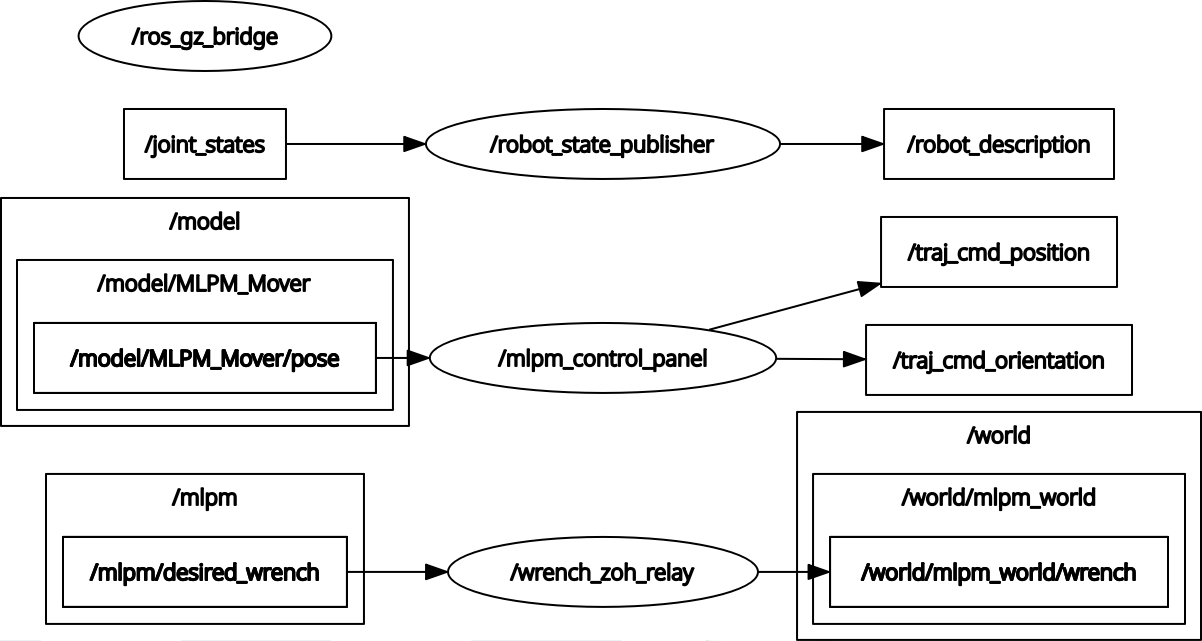
\includegraphics[width=0.95\textwidth]{img/ROS2_Topics.png}
	\caption{نمودار گراف محاسباتی ROS~2 در حین اجرای شبیه‌سازی MLPM}
	\label{fig:results-ros2-graph}
\end{figure}

همان‌طور که در شکل~\ref{fig:results-ros2-graph} مشاهده می‌شود، نودهای کلیدی عبارتند از:

\begin{itemize}
	\item \textbf{\lr{/mlpm\_control\_panel}}: نود اصلی کنترلر که مرجع مسیر را تولید و به MATLAB ارسال می‌کند
	\item \textbf{\lr{/wrench\_zoh\_relay}}: نود همگام‌ساز که خروجی کنترلر را با Zero-Order Hold نگه می‌دارد و تضمین می‌کند دستورات wrench بین نمونه‌های گسسته کنترلر پایدار بمانند
	\item \textbf{\lr{/ros\_gz\_bridge}}: چهار نمونه bridge برای انتقال Clock، Pose، Wrench و پارامترها بین Gazebo و ROS~2
	\item \textbf{\lr{/robot\_state\_publisher}}: انتشار توصیف هندسی ربات از URDF
\end{itemize}

تاپیک‌های کلیدی که در معماری ارتباطی نقش دارند در جدول~\ref{tab:results-ros-topics} خلاصه شده‌اند.

\begin{table}[htbp]
	\centering
	\caption{تاپیک‌های کلیدی ROS~2 در محیط شبیه‌سازی}
	\label{tab:results-ros-topics}
	\begin{tabular}{lll}
		\hline
		\textbf{تاپیک} & \textbf{نوع پیام} & \textbf{نقش} \\
		\hline
		\lr{/model/MLPM\_Mover/pose} & \lr{geometry\_msgs/Pose} & بازخورد وضعیت از Gazebo \\
		\lr{/world/mlpm\_world/wrench} & \lr{geometry\_msgs/Wrench} & اعمال نیرو/گشتاور به پلتفرم \\
		\lr{/mlpm/desired\_wrench} & \lr{geometry\_msgs/Wrench} & خروجی کنترلر قبل از ZOH \\
		\lr{/traj\_cmd\_position} & \lr{geometry\_msgs/Point} & مرجع موقعیت خطی \\
		\lr{/traj\_cmd\_orientation} & \lr{geometry\_msgs/Quaternion} & مرجع جهت‌گیری \\
		\hline
	\end{tabular}
\end{table}

\subsection{پیکربندی مدل فیزیکی}
\label{subsec:results-phys-config}

مدل URDF پلتفرم شناور با پارامترهای فیزیکی دقیق بارگذاری شد. جرم پلتفرم $m = 6.6~\text{kg}$ و ممان‌های اینرسی $I_{xx} = I_{yy} = 0.06~\text{kg·m}^2$ و $I_{zz} = 0.12~\text{kg·m}^2$ در فایل URDF تعریف شدند. هندسه بصری از مش STL آرایه Halbach با ضریب مقیاس $0.001$ استفاده می‌کند، در حالی که هندسه برخورد به صورت جعبه ساده‌شده با ابعاد $0.2286 \times 0.2286 \times 0.013~\text{m}$ برای کاهش بار محاسباتی فیزیک تعریف شده است.

موتور فیزیک DART با گام زمانی $\Delta t = 0.005~\text{s}$، شتاب گرانش $\mathbf{g} = [0, 0, -9.8]~\text{m/s}^2$، و ضریب اصطکاک زمین $\mu = 0.8$ پیکربندی شد. محدودیت‌های سرعت خطی ($10~\text{m/s}$) و زاویه‌ای ($5~\text{rad/s}$) برای جلوگیری از واگرایی عددی اعمال شدند.

\subsection{معیارهای اعتبارسنجی}
\label{subsec:results-validation-criteria}

برای تأیید صحت عملکرد محیط شبیه‌سازی، موارد زیر بررسی شد:

\begin{enumerate}
	\item \textbf{بارگذاری مدل URDF}: ربات با پارامترهای جرمی و اینرسی صحیح در Gazebo spawn شد و در ارتفاع اولیه $z = 4.0~\text{m}$ قرار گرفت.
	
	\item \textbf{همگام‌سازی Clock}: تمام نودهای ROS~2 با تاپیک \lr{\texttt{/clock}} شبیه‌ساز همگام بودند و زمان شبیه‌سازی به درستی منتشر می‌شد.
	
	\item \textbf{بازخورد وضعیت}: پلاگین \lr{\texttt{PosePublisher}} وضعیت پلتفرم را با فرکانس $60~\text{Hz}$ منتشر می‌کرد و داده‌ها از طریق \lr{\texttt{parameter\_bridge}} به MATLAB منتقل می‌شدند.
	
	\item \textbf{اعمال نیرو/گشتاور}: دستورات wrench از MATLAB به تاپیک \lr{\texttt{/world/mlpm\_world/wrench}} منتقل و توسط پلاگین \lr{\texttt{ApplyLinkWrench}} به \lr{\texttt{base\_link}} اعمال می‌شدند.
	
	\item \textbf{همگام‌سازی گسسته-پیوسته}: نود \lr{\texttt{wrench\_zoh\_relay}} با استفاده از شماره توالی (\lr{seq}) دستورات جدید را تشخیص داده و با Zero-Order Hold آن‌ها را بین نمونه‌های کنترلر نگه می‌داشت.
	
	\item \textbf{پایداری عددی}: محدودیت‌های سرعت و گام زمانی کوچک از واگرایی عددی جلوگیری کردند و شبیه‌سازی در تمام سناریوهای آزمایش پایدار ماند.
\end{enumerate}

این آزمون‌ها تأیید کردند که محیط شبیه‌سازی آماده ارزیابی الگوریتم‌های کنترلی است و معماری ارتباطی برای انتقال به سخت‌افزار واقعی در آینده مناسب است.

\section{ارزیابی عملکرد کنترلر فازی-PID}
\label{sec:results-fuzzy-pid}

با کسب اطمینان از ارتباط صحیح، هماهنگ و دقیق بین محیط نرم‌افزار MATLAB و فضای شبیه‌سازی Gazebo، می‌توان از شبیه‌ساز حاصل به مثابه سیستمی واقعی بهره برد و کنترلر طراحی‌شده را در زمان آزمایش ارزیابی نمود. با توجه به ساختار شش درجه آزادی سیستم، در این بخش برای هر یک از این درجات، ابتدا شبیه‌ساز راه‌اندازی شده و سپس با اعمال ورودی پله با دامنه مناسب و در محدوده مجاز فضای کاری، پاسخ سیستم استخراج و ضبط می‌شود.

وجود این بستر شبیه‌سازی جامع و امکان دریافت و ذخیره‌سازی داده‌ها از بخش‌های مختلف آن، قابلیت بررسی چندجانبه عملکرد سیستم را در هر آزمایش فراهم کرده است. از این رو، نتایج در سه دسته اصلی شامل «عملکرد ردیابی»، «رفتار تطبیقی کنترلر»، و «تلاش کنترلی و تخصیص جریان» ارائه می‌شوند. در روند هر آزمایش، علاوه بر بررسی نمودار پاسخ پله در تقابل با سیگنال مرجع، سایر متغیرهای کلیدی نیز تحلیل می‌گردند؛ این متغیرها شامل نمودارهای تغییرات ضرایب کنترلر PID
(که به وسیله بلوک فازی تنظیم می‌شوند)، میزان تلاش کنترلی تولیدشده توسط کنترلر و در نهایت، جریان‌های الکتریکی ایجادشده در هر یک از سیم‌پیچ‌ها می‌باشد.

%====================================================
\subsection{عملکرد ردیابی سیستم}
\label{subsec:results-tracking}

با اعمال ورودی پله، انتظار می‌رود بخش متحرک سیستم مسیر یا زاویه مطلوب را در کمترین زمان ممکن طی کند و عملکرد آن از منظر شاخص‌های رایج کنترلی نظیر فراجهش، زمان خیز، زمان نشست و خطای حالت ماندگار در وضعیت بهینه‌ای قرار داشته باشد. برای دستیابی به چنین پاسخی، خروجی‌های بلوک کنترل فازی باید به محدوده‌ای از مقادیر پایدار به عنوان ضرایب کنترل‌کننده PID نگاشت شوند.

اگرچه در این ساختار ضرایب کنترلی به صورت پیوسته متغیر هستند، اما یافتن بازه مناسب برای آن‌ها، مشابه فرآیند تنظیم (Tuning) یک کنترل‌کننده PID کلاسیک، نیازمند تکرار، بررسی و سعی و خطا بر روی پاسخ‌های سیستم به ازای مقادیر ثابت است. پس از تعیین این محدوده‌های پایه که عملکرد اولیه و قابل‌قبولی ارائه می‌دهند، کنترل‌کننده فازی با اعمال رفتار تطبیقی خود (که مکانیزم آن در فصل پیشین تشریح شد)، بهینه‌سازی نهایی و لحظه‌ای پاسخ سیستم را بر عهده می‌گیرد.

بنابراین، در این بخش ابتدا محدوده‌های به‌دست‌آمده برای نگاشت ضرایب به ازای هر یک از درجات آزادی معرفی شده و سپس پاسخ‌های استخراج‌شده بر اساس این ضرایب، به صورت عددی و تصویری مورد ارزیابی دقیق قرار خواهند گرفت.
%----------------------------------------------------
\subsubsection{پاسخ پله درجات آزادی خطی ($X$, $Y$, $Z$)}
\label{subsubsec:results-linear-step}
به منظور اعمال پله به درجات خطی سیستم، با توجه به اینکه تابع تبدیلی از سیستم در اختیار نیست و علاوه بر این مقدار واحد به معنای عدد 1 در ابعاد فضای کاری سیستم نمی گنجد، بنابراین تنها پاسخ های پله از سیستم گرفته شده و این پاسخ ها، به پله ی واحد نیستند. 
با تعریف فضای کاری به صورت سطحی با 40*40 سانتی متر طول و عرض و امکان جابه جایی عمودی مرکز ثقل سیستم از ارتفاع 16 میلیمتر تا 35 میلیمتر، پله های اعمال شده به سیستم در این بازه قرار داشته است. برای محور x و y این پله از نقطه ی 0 تا 10 سانتی متر، و برای محور z از 16 میلیمتر تا 30 میلیمتر طراحی شده است. با این حال لازم است یادآوری شود که پارامتر های استخراج شده برای مدل عملگر تنها در ارتفاع ثابتی از متحرک طراجی شده اند و در نتیجه علی رغم امکان کنترل موقعیت متحرک در ارتفاع های مختلف، به صورت عملی این ارتفاع باید در مقدار مشخصی ثابت نگه داشته شود و از این رو، پاسخ پله ی دریافت شده تنها در محیط شبیه سازی قابل اعمال و اندازه گیری می باشد. 
در ادامه، به بررسی درجات آزادی خطی و رفتار آنها پس از ورودی پله پرداخته می شود. 

\paragraph{محورهای $X$ و $Y$}
با توجه به ساختار متقارن و دوگانه‌ی دستگاه در راستاهای $X$ و $Y$، طراحی کنترل‌کننده برای این دو محور از ساختار و محدوده‌ی ضرایب یکسانی بهره می‌برد. با این وجود، به دلیل تفاوت در جهت برهم‌کنش میدان‌های مغناطیسی سیم‌پیچ‌ها با آرایه‌ی آهنربای بخش متحرک، پاسخ‌های دینامیکی حاصل برای این دو محور اندکی با یکدیگر متفاوت است. ضرایب محاسبه‌شده برای نگاشت خروجی‌های فازی به ضرایب PID این دو محور در بازه‌های زیر تعریف شده‌اند:

\begin{align}
	K_p &\in \text{\lr{[0, 50]}} \\
	K_i &\in \text{\lr{[0, 1.6]}} \\
	K_d &\in \text{\lr{[0, 40]}}
\end{align}

پاسخ‌های پله‌ی حلقه‌بسته برای این دو محور در شکل \ref{fig:results-xy-step} نشان داده شده است.

\begin{figure}[htbp]
	\centering
	\subfloat[محور $X$]{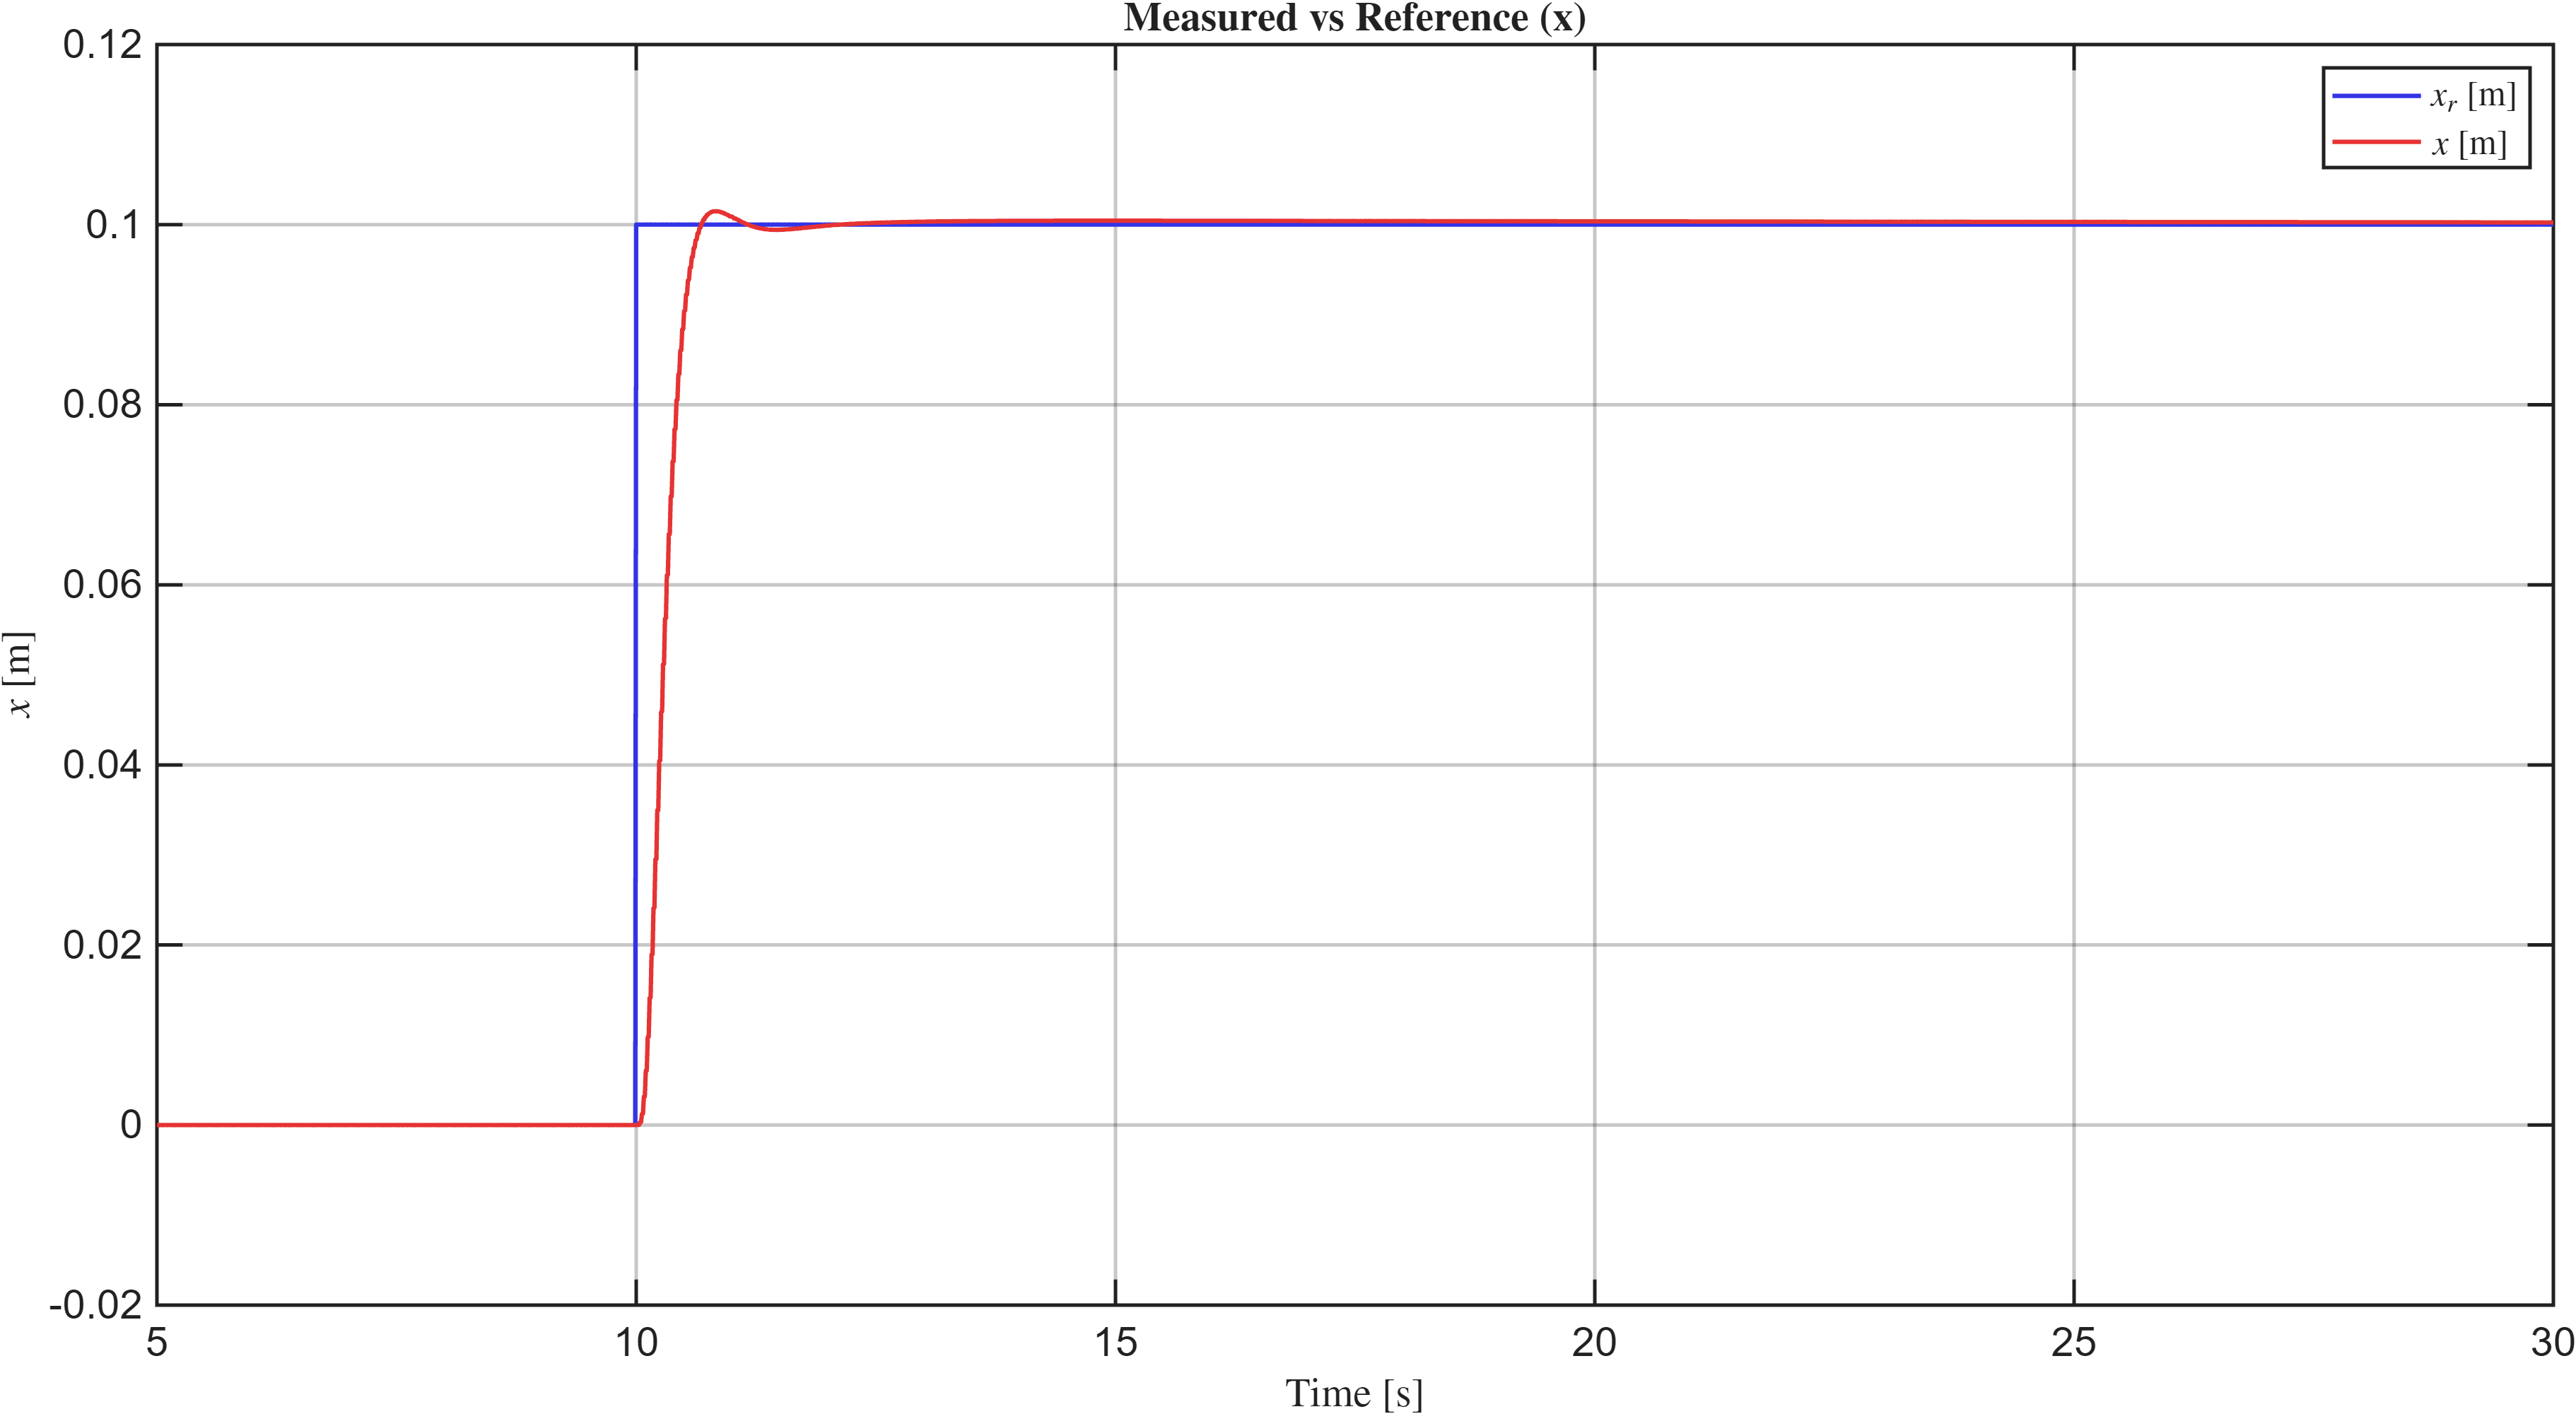
\includegraphics[width=0.48\textwidth]{img/step/x/pose-compare-x}}
	\hfill
	\subfloat[محور $Y$]{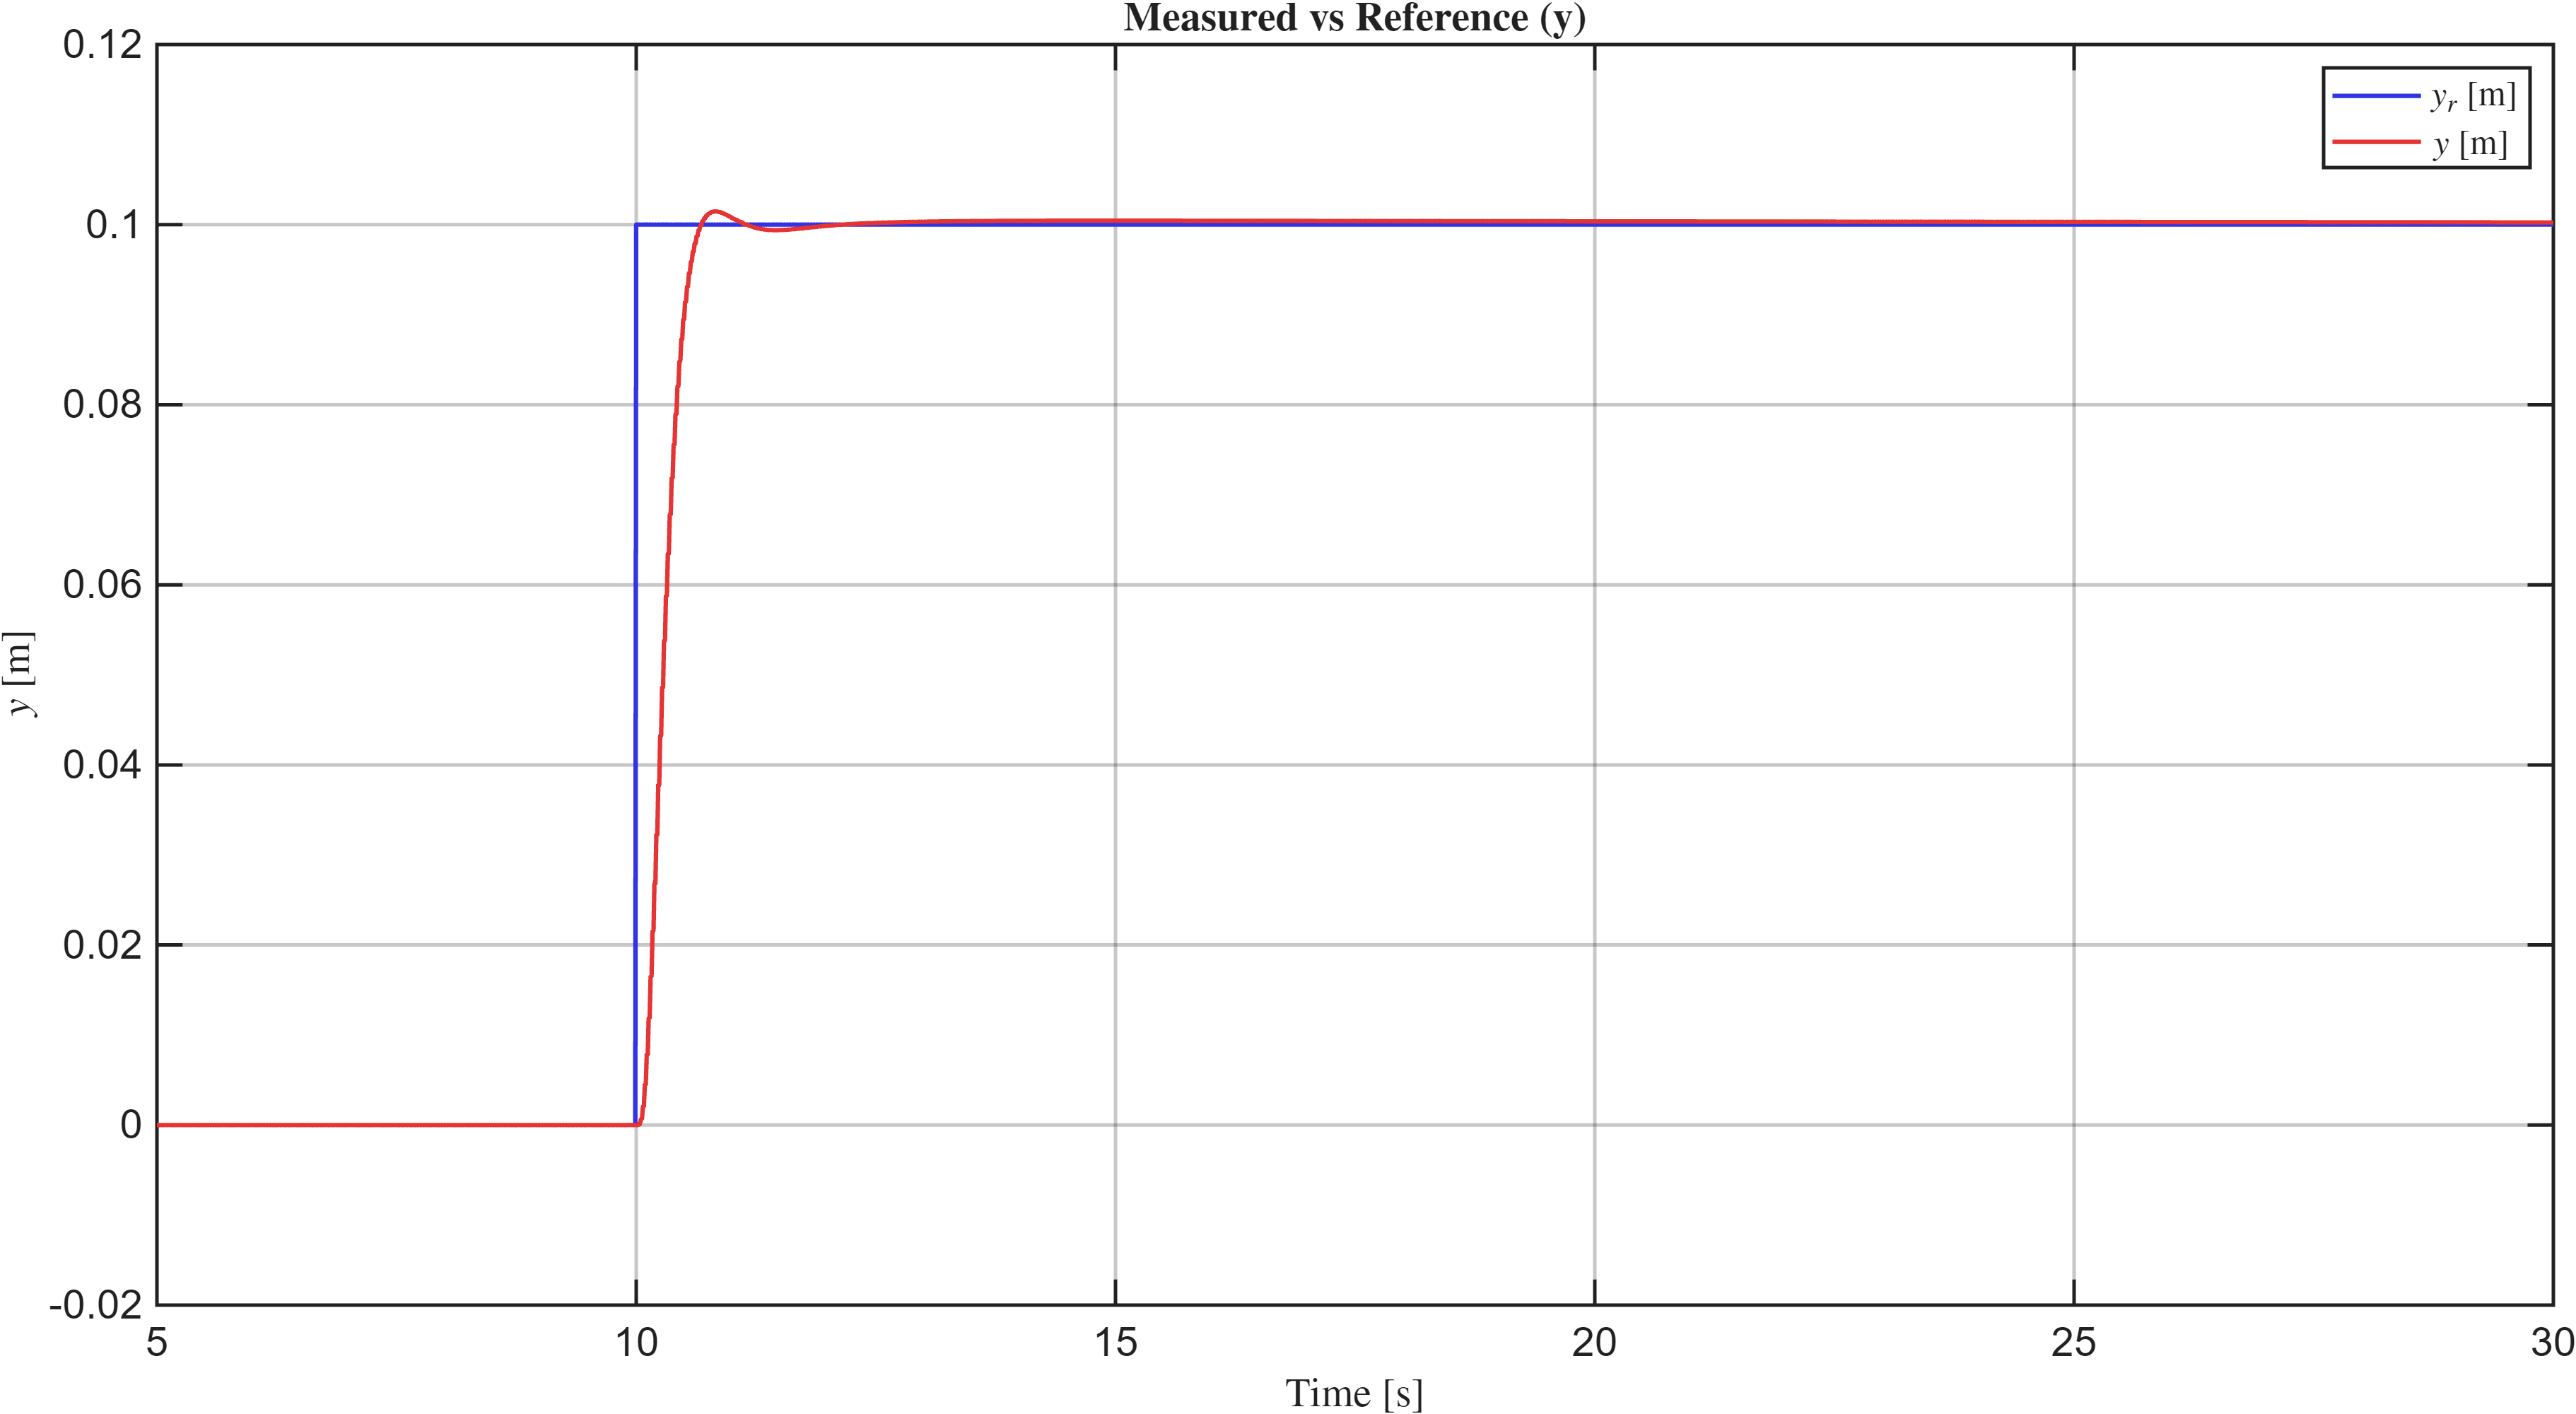
\includegraphics[width=0.48\textwidth]{img/step/y/pose-compare-y}}
	\caption{پاسخ پله درجات آزادی خطی در محورهای $X$ و $Y$}
	\label{fig:results-xy-step}
\end{figure}

%----------------------------------------------------
\paragraph{محور $Z$}
بازه‌ی ضرایب کنترل‌کننده‌ی محور عمودی $Z$ مشابه محورهای صفحه‌ای تعیین شده است، اما مقادیر آن‌ها به مراتب بزرگ‌تر انتخاب شده‌اند. دلیل این امر، نیاز به غلبه بر نیروی وزن جرم متحرک در این راستا است. برای پاسخ‌دهی مناسب به تغییرات ارتفاع، کنترل‌کننده باید نیرویی متناسب با اینرسی جسمی به جرم $6.6$ کیلوگرم تأمین نماید. بازه‌ی جستجوی ضرایب به صورت زیر تعریف شده است:

\begin{align}
	K_p &\in \text{\lr{[0, 367.5]}} \\
	K_i &\in \text{\lr{[0, 70]}} \\
	K_d &\in \text{\lr{[0, 490]}}
\end{align}

پاسخ پله‌ی حلقه‌بسته‌ی این کنترل‌کننده در شکل \ref{fig:results-z-step} نمایش داده شده است.

\begin{figure}[htbp]
	\centering
	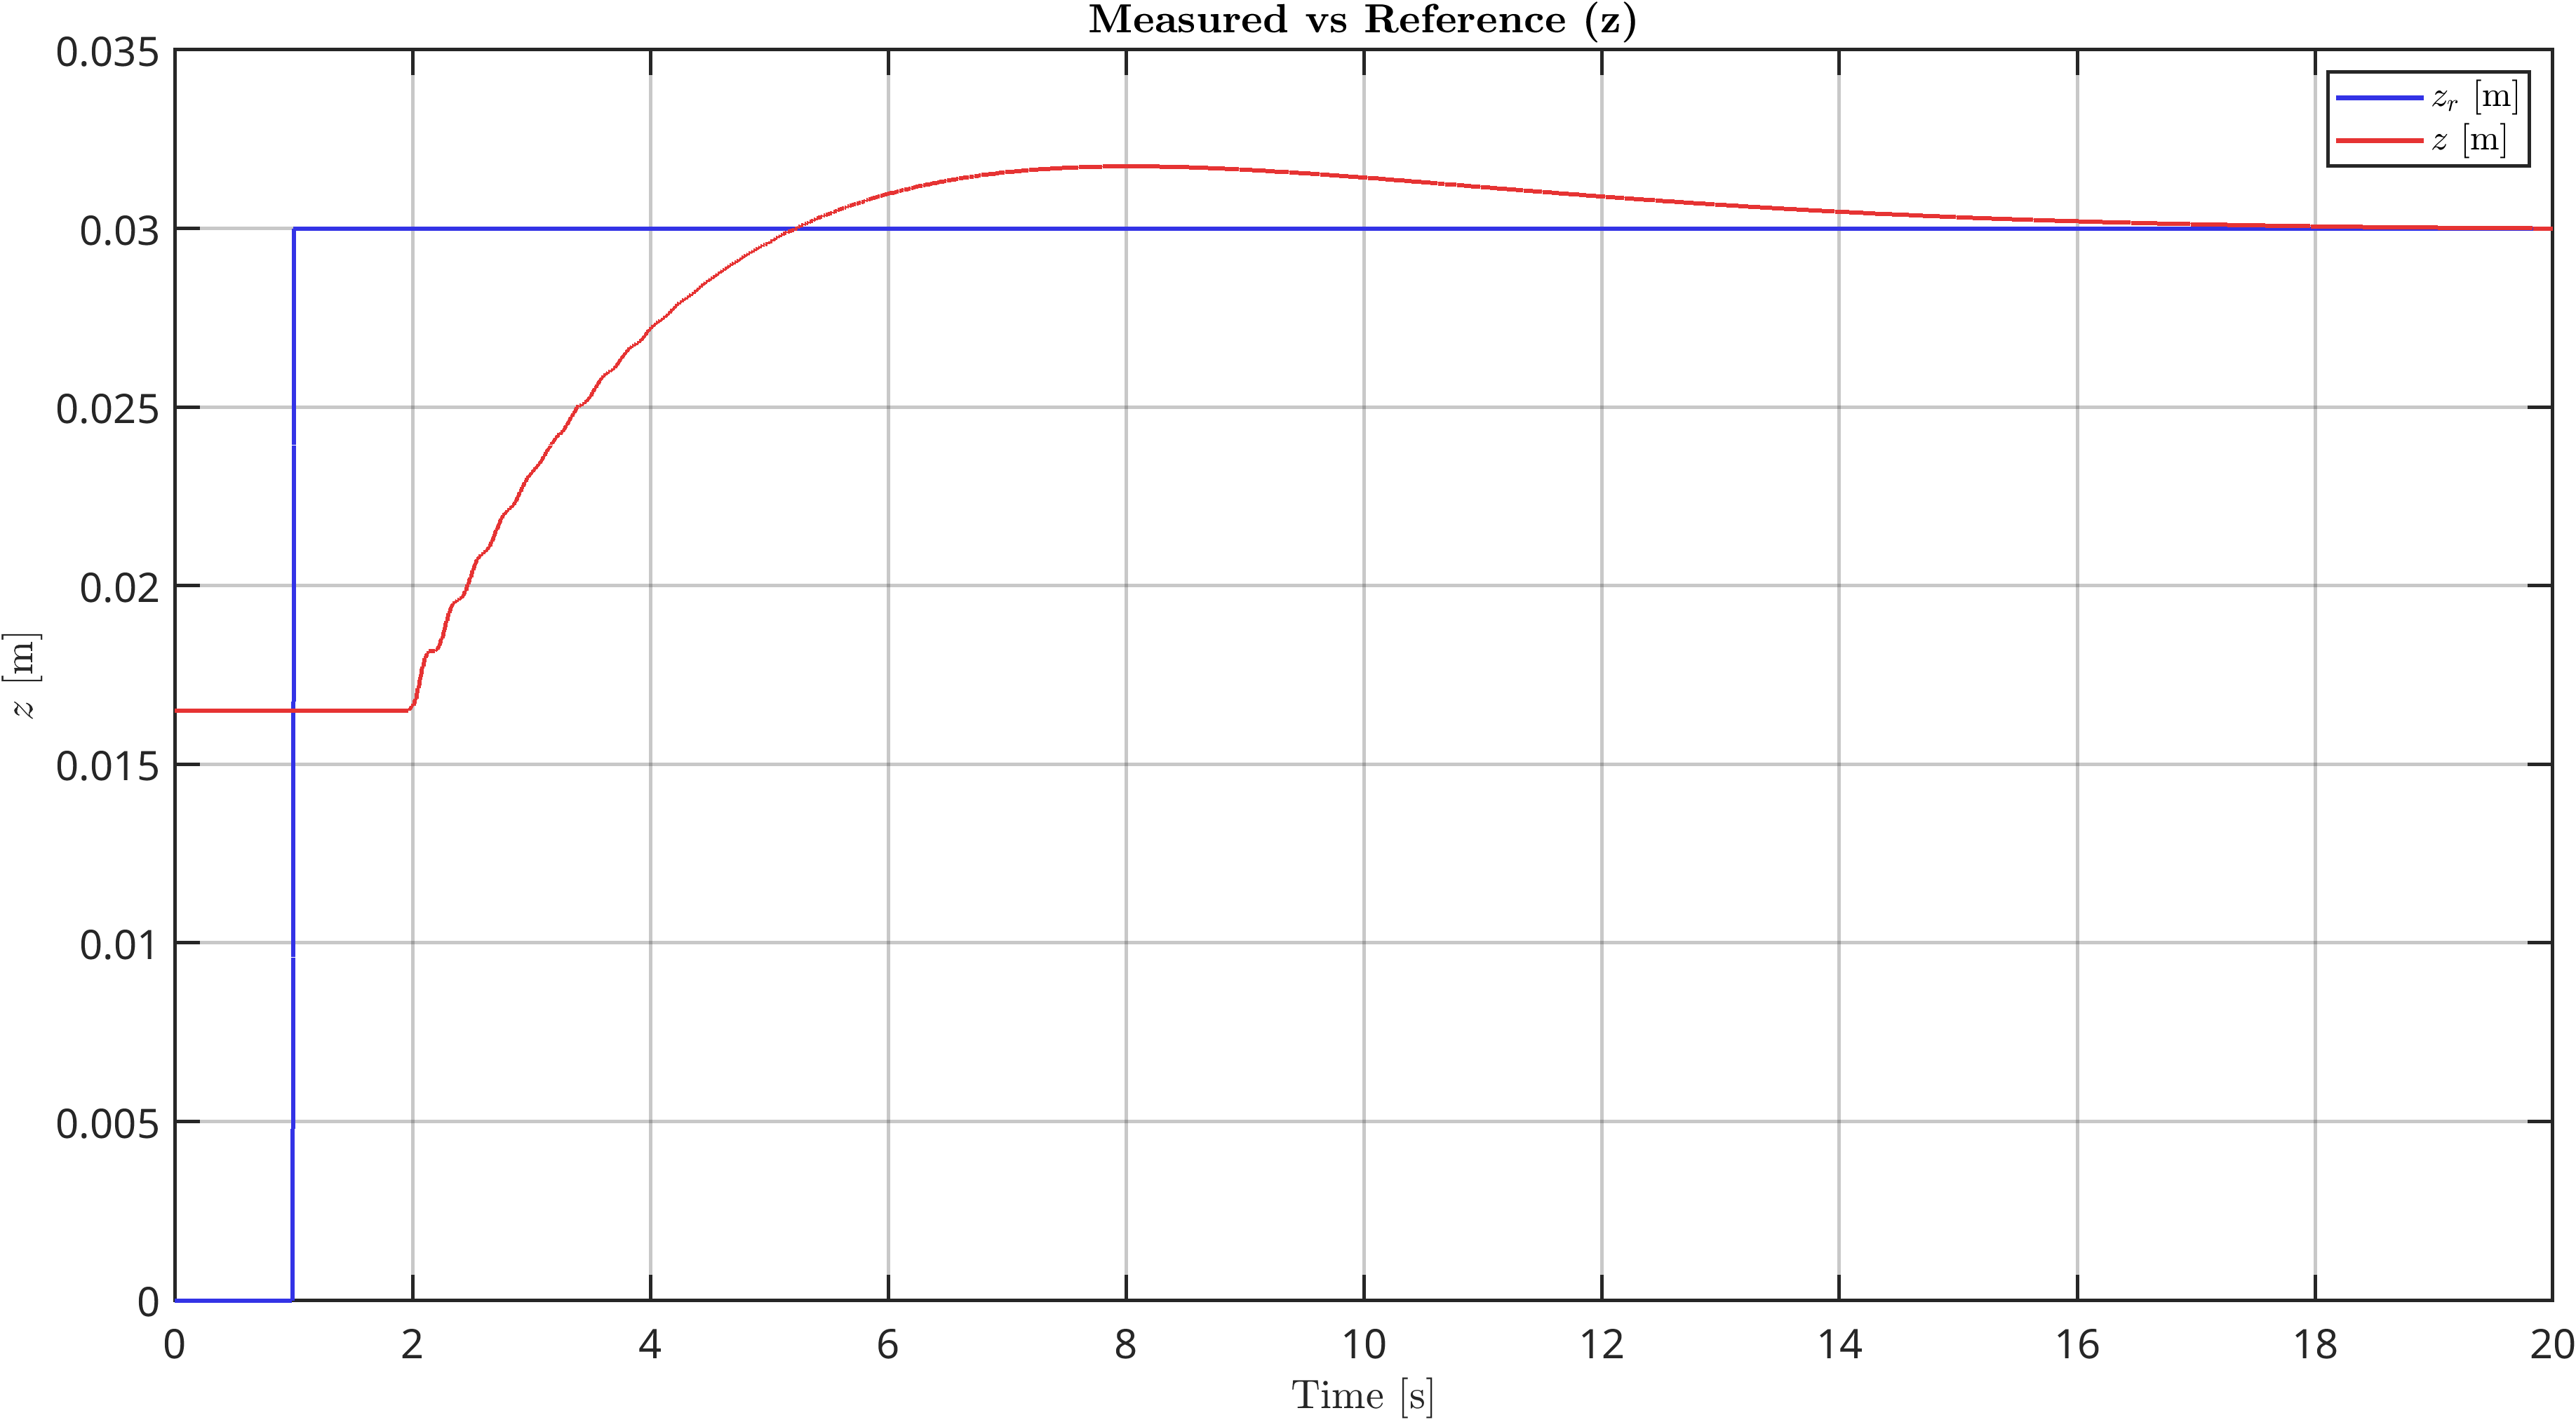
\includegraphics[width=0.75\textwidth]{img/step/z/pose-compare-z}
	\caption{پاسخ پله درجه آزادی خطی در محور $Z$}
	\label{fig:results-z-step}
\end{figure}

%----------------------------------------------------

ارزیابی کمّی عملکرد کنترل‌کننده‌ها برای درجات آزادی خطی در جدول \ref{tab:results-linear-metrics} ارائه شده است. نتایج به‌دست‌آمده برای محورهای $X$ و $Y$، بیان‌گر هم‌گرایی نزدیک به یکدیگر و عملکرد کاملاً رضایت‌بخش در صفحه‌ی افقی است. زمان خیز در حدود $0.37$ ثانیه، زمان نشست نزدیک به $1.12$ ثانیه و فراجهش کمتر از $1.25$ درصد، در کنار خطای ماندگار در مرتبه‌ی $10^{-4}$ متر، گواهی بر پاسخ سریع، میرایی مناسب و دقت بالای کنترل‌کننده در این دو راستا است. مقادیر کم فراجهش نشان می‌دهد که سیستم بدون نوسان اضافی به سرعت به مقدار مرجع هم‌گرا می‌شود.

این عملکرد مطلوب در صفحه‌ی افقی، تضمین‌کننده‌ی لازم برای مأموریت اصلی دستگاه یعنی تعقیب مسیرهای صفحه‌ای با حداکثر سرعت و دقت خواهد بود. از سوی دیگر، تحلیل عملکرد محور $Z$ بیان‌گر چالش‌های ذاتی کنترل در راستای عمود است. زمان خیز بلندتر ($3.45$ ثانیه) و زمان نشست به مراتب طولانی‌تر ($12.80$ ثانیه) در این محور، ریشه در اینرسی بیشتر و ضرورت غلبه بر گرانش دارد. با این وجود، فراجهش محدود به $5.79$ درصد و خطای ماندگار بسیار کوچک (در حدود $7.8 \times 10^{-6}$ متر) نشان می‌دهد که کنترل‌کننده با وجود کندی نسبی، توانسته است ارتفاع را با دقت بسیار خوبی به نقطه‌ی کار مطلوب برساند. با توجه به ثابت بودن ارتفاع هدف در این پروژه و نیاز صرف به رفع اغتشاش در این راستا، این عملکرد پایدار و دقیق، رضایت‌بخش ارزیابی می‌شود.

\begin{table}[htbp]
	\centering
	\caption{شاخص‌های عملکرد پاسخ پله برای محورهای $X$، $Y$ و $Z$}
	\label{tab:results-linear-metrics}
	\begin{tabular}{c c c c c c c}
		\toprule
		محور & زمان خیز & زمان نشست & فراجهش & زمان اوج & خطای ماندگار & RMSE \\
		\midrule
		$X$ & \lr{0.36842} & \lr{1.1192} & \lr{1.2408} & \lr{1.32} & \lr{0.00024687} & \lr{0.0086346} \\
		$Y$ & \lr{0.37847} & \lr{1.1239} & \lr{1.2056} & \lr{1.33} & \lr{0.00024818} & \lr{0.0086324} \\
		$Z$ & \lr{3.4484} & \lr{12.795} & \lr{5.7908} & \lr{7.51} & \lr{$7.8361 \times 10^{-6}$} & \lr{0.0054485} \\
		\bottomrule
	\end{tabular}
\end{table}

%----------------------------------------------------
\subsubsection{پاسخ پله درجات آزادی زاویه‌ای ($\alpha$، $\beta$، $\gamma$)}
\label{subsubsec:results-angular-step}

اعمال ورودی پله به درجات آزادی زاویه‌ای سامانه‌ی MLPM با چالش‌هایی همراه است که در این بخش به آن‌ها پرداخته می‌شود. فضای کاری زاویه‌ای این جسم، بازه‌ی تغییرات مجاز برای زوایای $\alpha$ و $\beta$ را به حدود $\pm 5$ درجه محدود می‌کند. بر این اساس، ورودی پله‌ی اعمالی به صفحه‌ی متحرک برای این دو درجه آزادی، پله‌ای به اندازه‌ی $0$ تا $0.07$ رادیان (معادل $4$ درجه) در نظر گرفته شده است.

همان‌گونه که در تحلیل تکینگی سامانه بیان شد، درجه آزادی $\gamma$ در زوایای $\pm \pi/2$ و $\pm\pi$ به دلیل هم‌راستایی میدان‌های مغناطیسی بخش متحرک و ثابت، دچار تکینگی می‌شود و شبیه‌سازی با شکست مواجه می‌گردد. از این رو، در آزمون‌های کنترل و بدون به‌کارگیری راهبردهایی برای عبور از نقاط تکین، حرکت در این راستا تنها در بازه‌هایی به دور از تکینگی امکان‌پذیر است. بر این اساس، پله‌ی اعمالی برای محور $\gamma$ از $\pi/4$ تا $\pi/4 + \pi/16$ تعریف و استفاده شده است. در ادامه به تشریح پاسخ های پله و بررسی عملکرد کنترل کننده در این سه راستا پرداخته می شود. 

\paragraph{محورهای $\alpha$ و $\beta$}
با توجه به تقارن ساختاری و دینامیکی دستگاه در دو جهت زاویه‌ای $\alpha$ و $\beta$، بازه‌ی ضرایب کنترل‌کننده‌ی مورد استفاده برای این دو محور یکسان بوده و به صورت زیر تعریف می‌شود:

\begin{align}
	K_p &\in \text{\lr{[0, 2.5]}} \\
	K_i &\in \text{\lr{[0, 1]}} \\
	K_d &\in \text{\lr{[0, 1]}}
\end{align}

محدوده‌ی نسبتاً کوچک این ضرایب در قیاس با محورهای خطی، ناشی از گشتاورهای اینرسی کمتر و حساسیت بالاتر سامانه در درجات آزادی زاویه‌ای است. پاسخ پله‌ی زاویه‌ای این دو محور در شکل \ref{fig:results-alpha-beta-step} نشان داده شده است.

\begin{figure}[htbp]
	\centering
	\subfloat[محور $\alpha$]{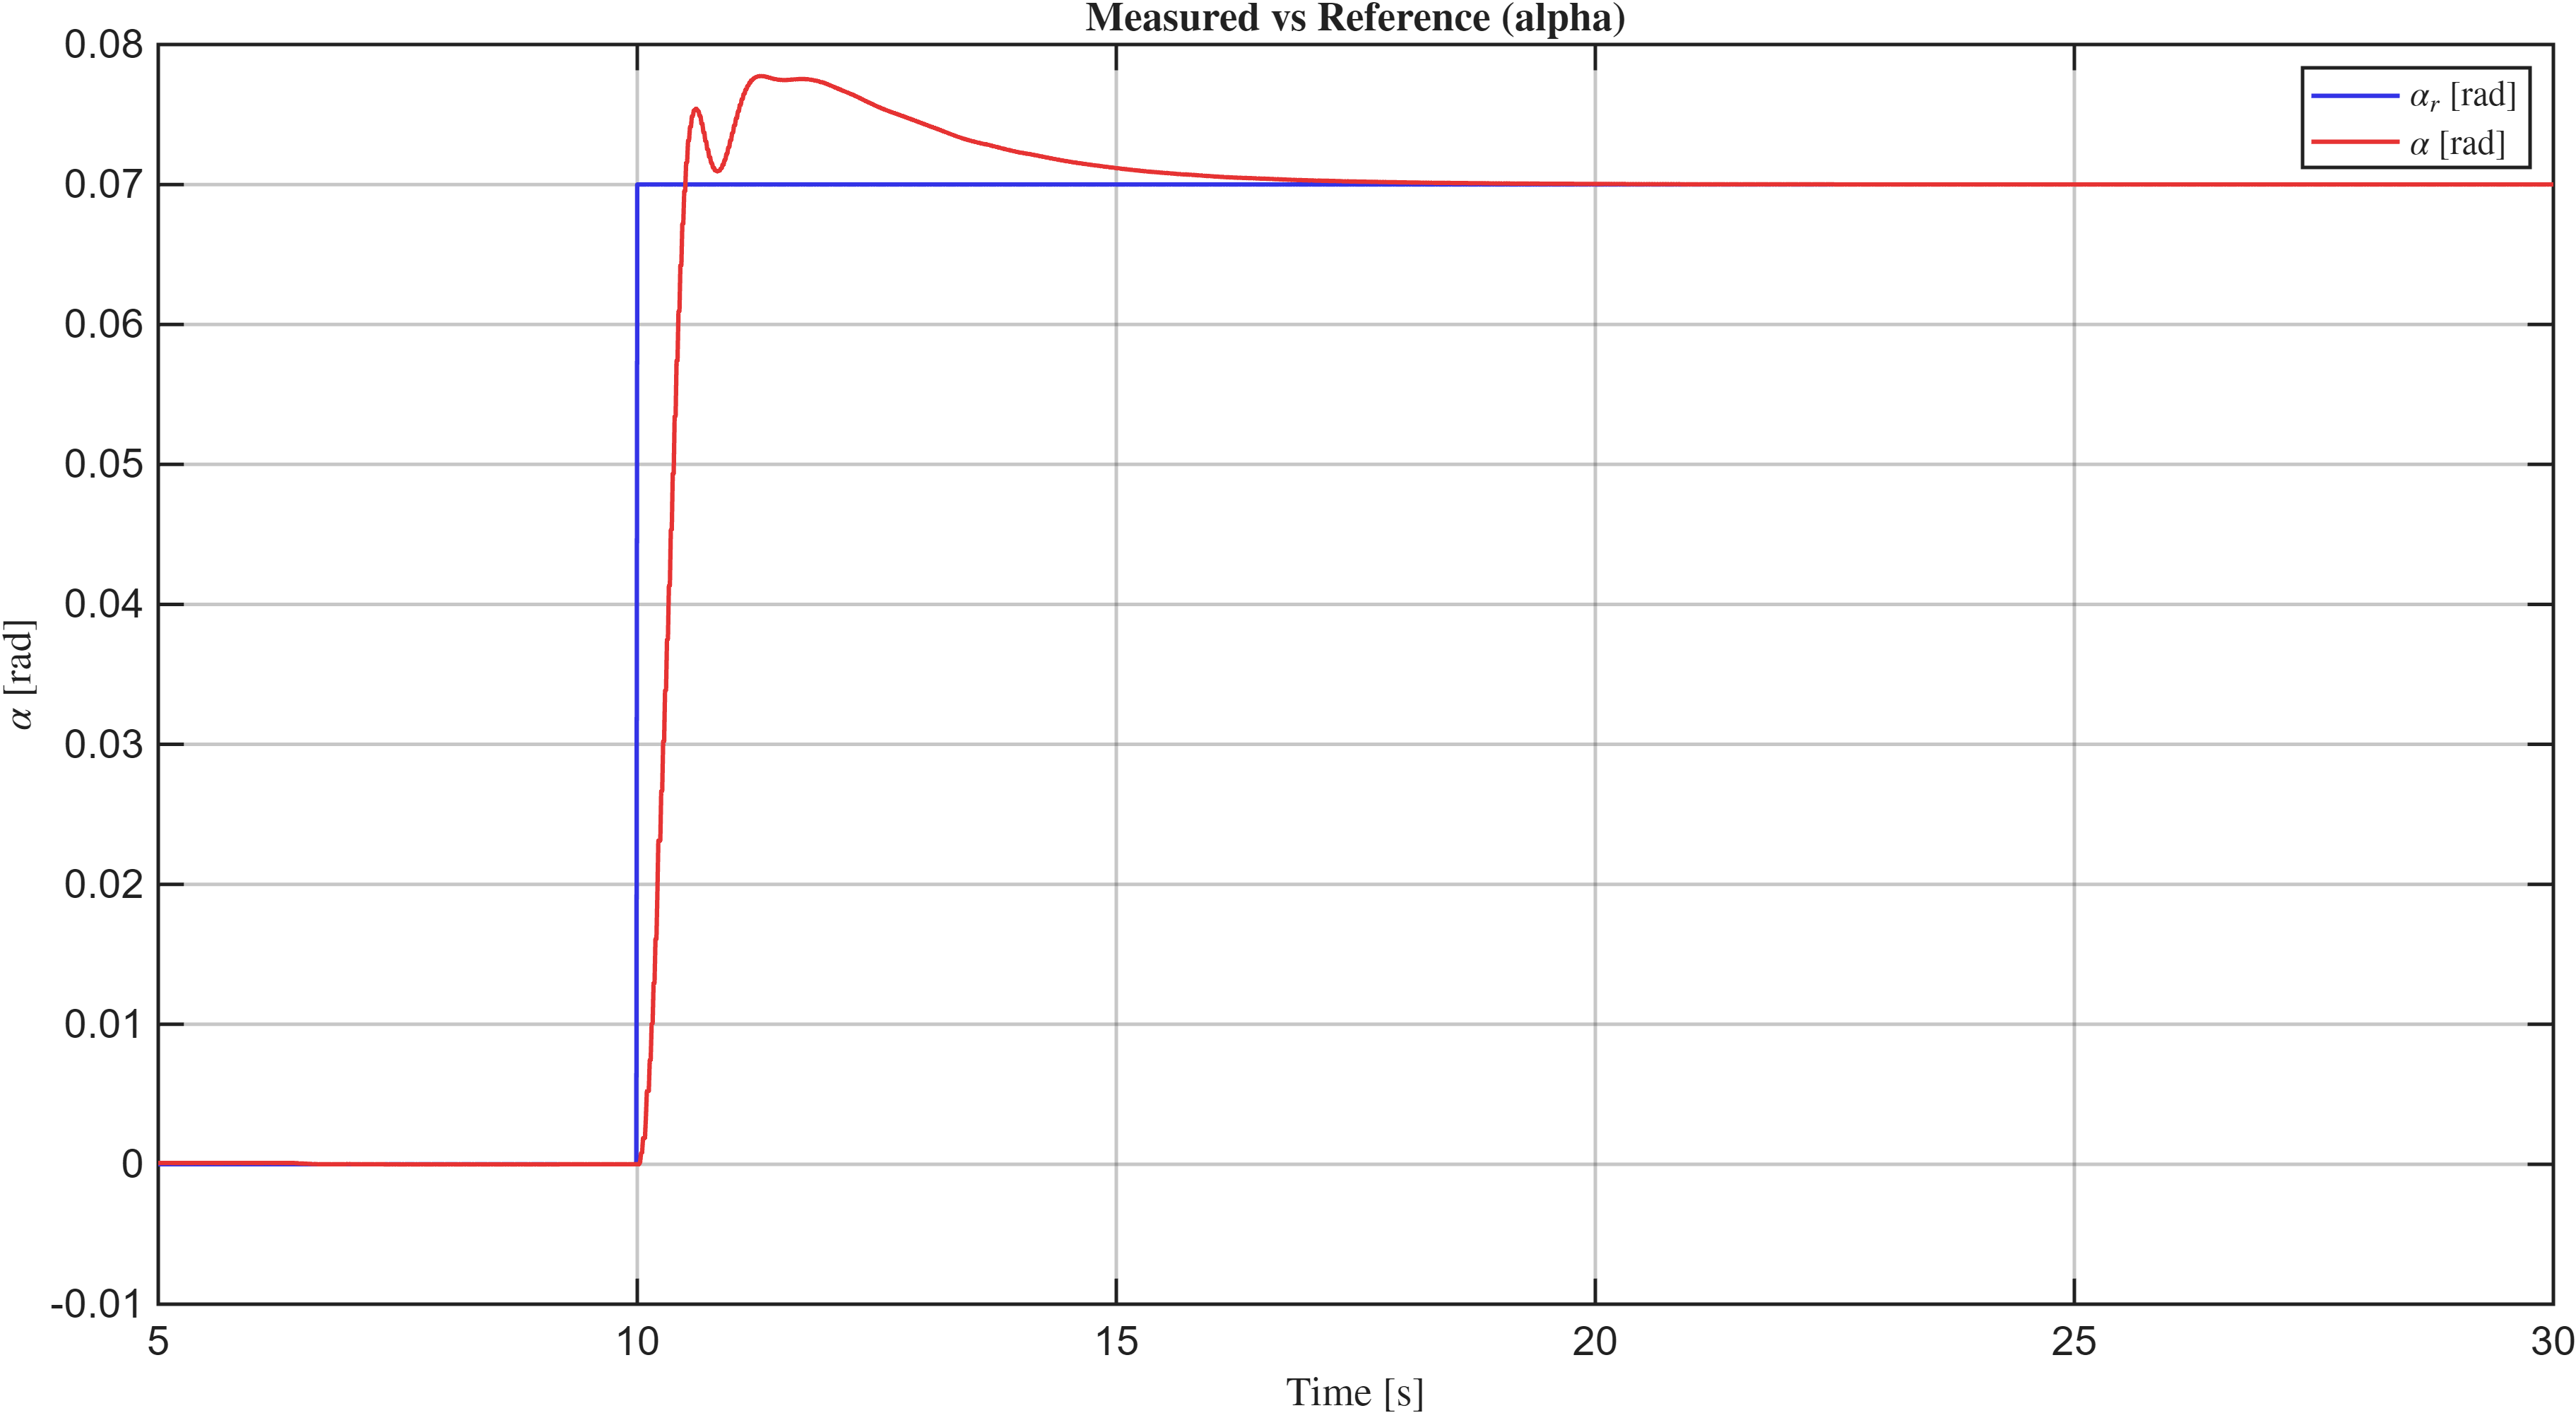
\includegraphics[width=0.48\textwidth]{img/step/alpha/pose-compare-alpha}}
	\hfill
	\subfloat[محور $\beta$]{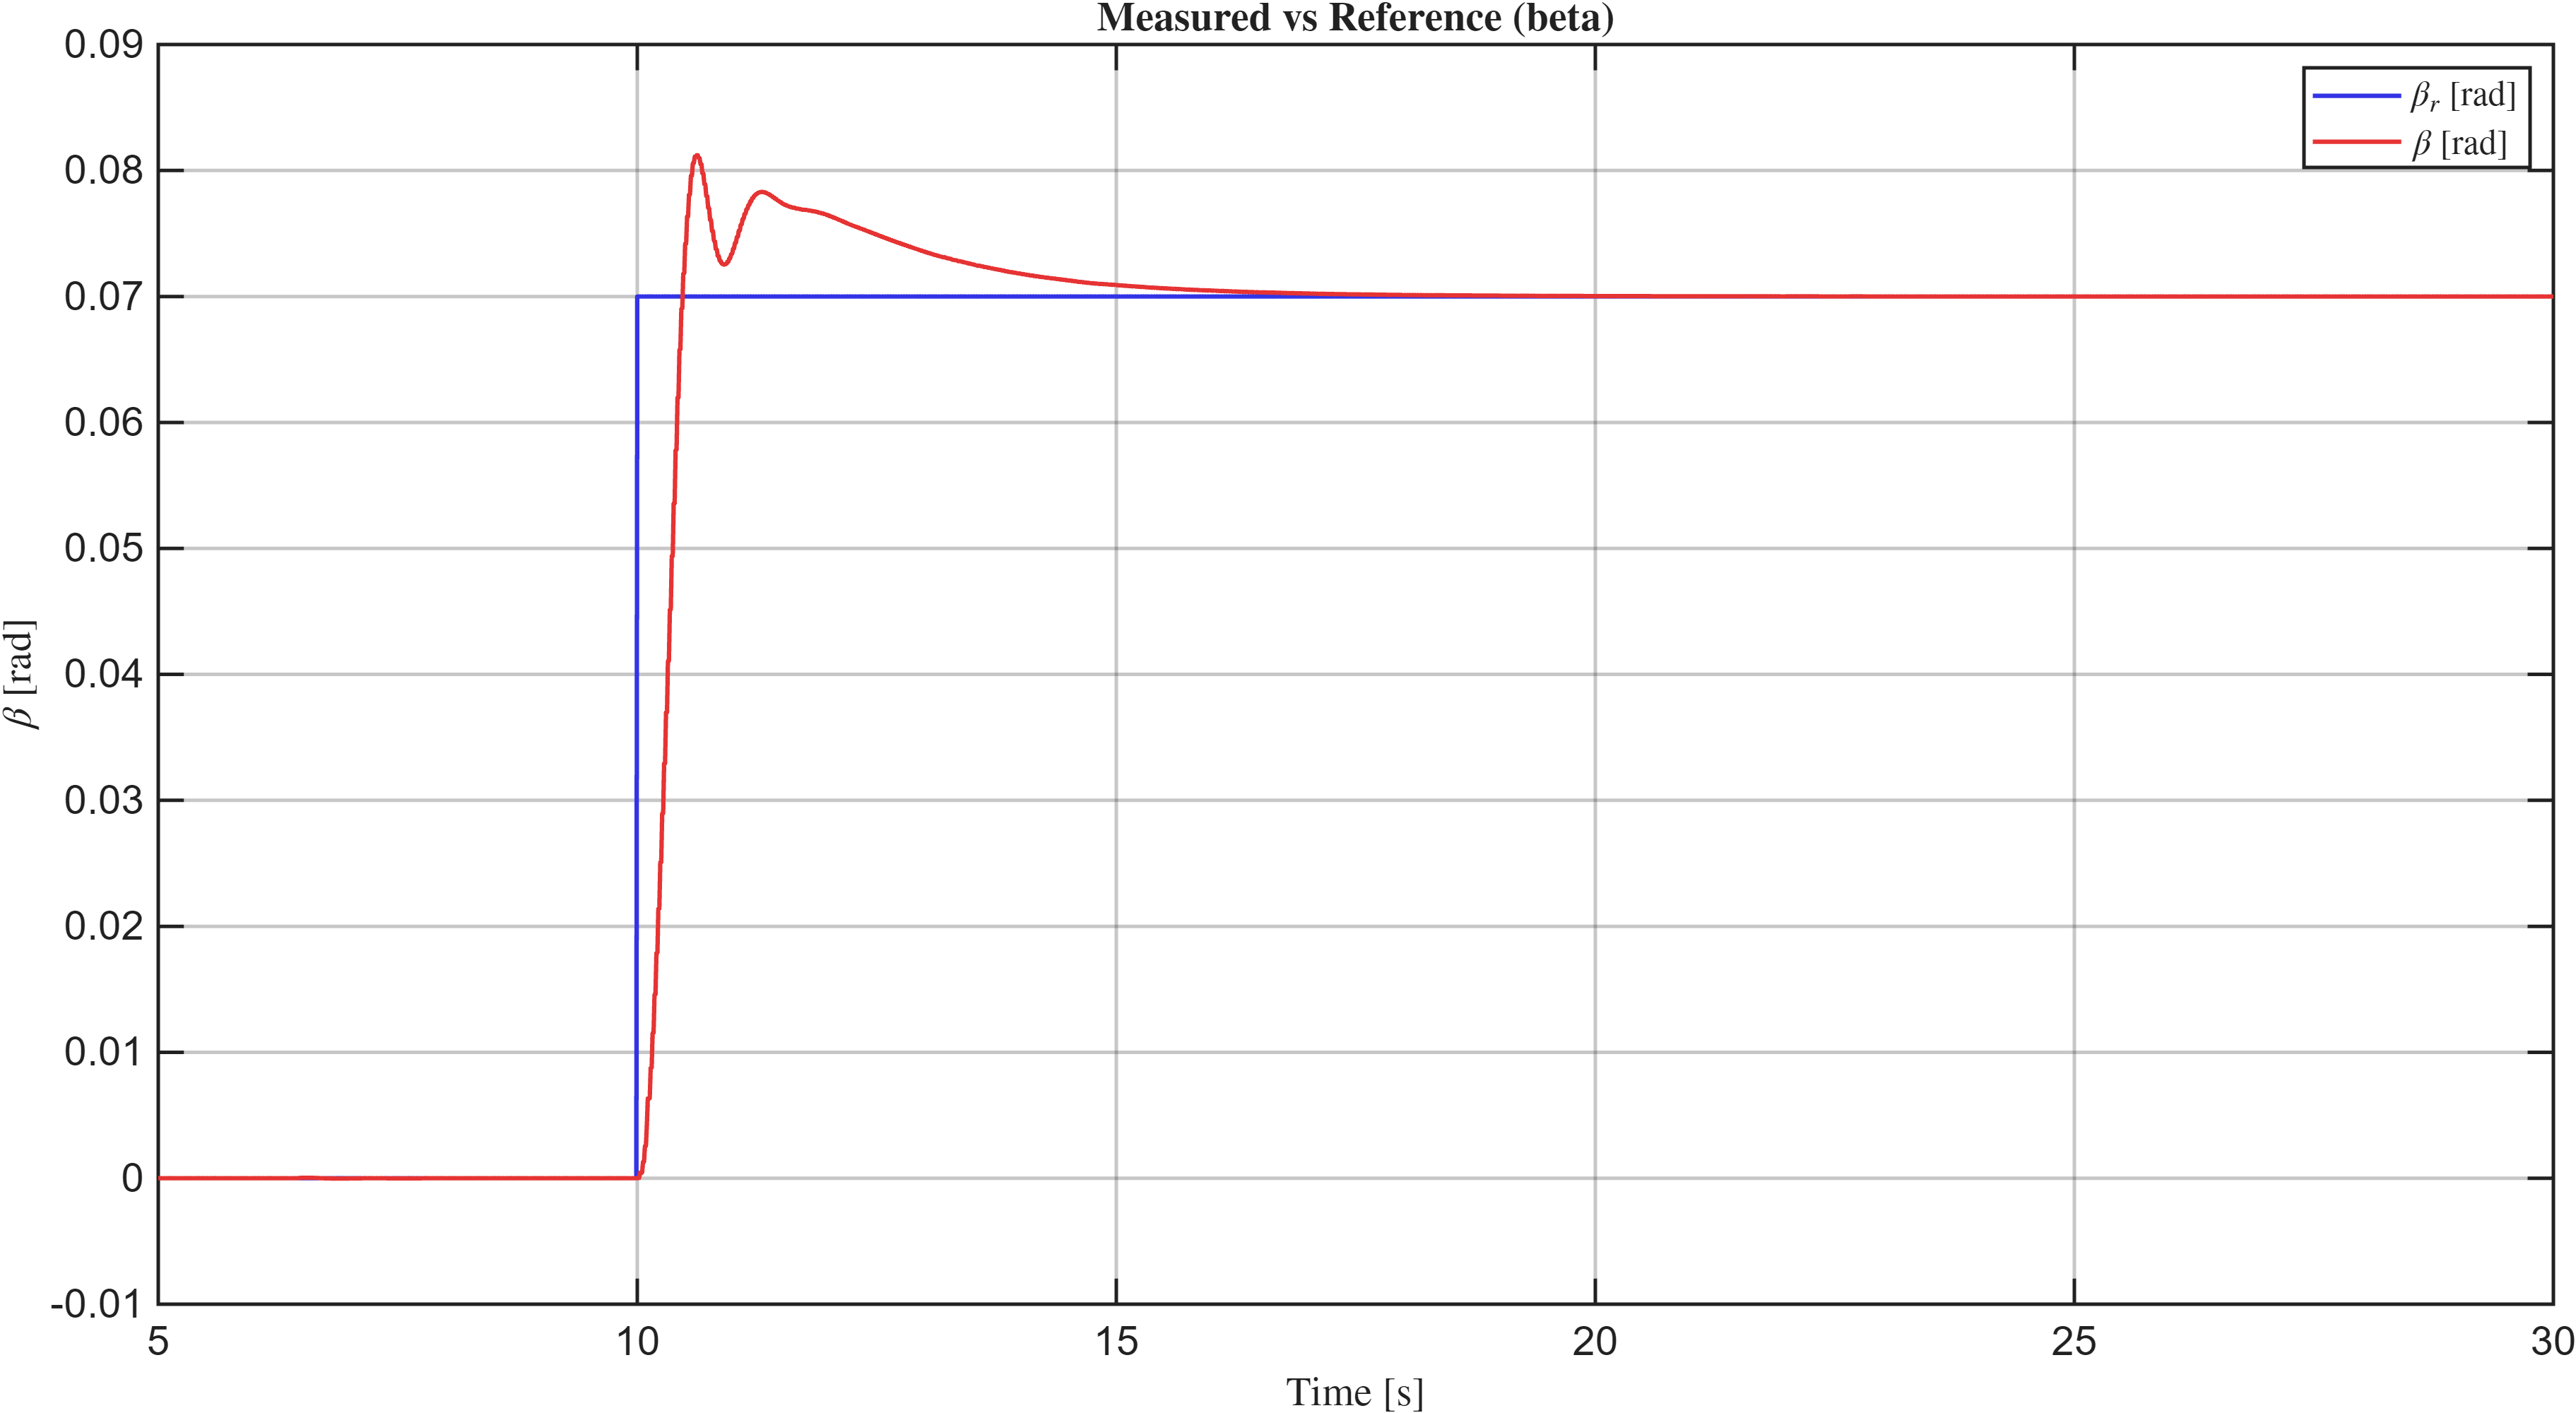
\includegraphics[width=0.48\textwidth]{img/step/beta/pose-compare-beta}}
	\caption{پاسخ پله زاویه‌ای محورهای $\alpha$ و $\beta$}
	\label{fig:results-alpha-beta-step}
\end{figure}

با این حال، مشابه آنچه که در دو راستای x و y مشاهده شد، علی رغم تشابه رفتار دو راستا، تفاوت های نیز در شکل پاسخ ها دیده می شود که علی رغم تفاوت در شکل پاسخ، دارای ویژگی های کنترلی نزدیک و مشابهی هستند. 
\paragraph{محور $\gamma$}
به دلیل تفاوت قابل توجه ممان اینرسی زاویه‌ای محور $\gamma$ نسبت به دو محور $\alpha$ و $\beta$، تعیین بازه‌ی ضرایب کنترل‌کننده‌ی PID برای این درجه آزادی نیازمند تنظیماتی متمایز است. در این فرایند، کنترل‌کننده باید پیش از رسیدن به محدوده‌ی مجاز حرکت، به پاسخی پایدار همگرا شود و هم‌زمان سرعت پاسخ مناسبی نیز ارائه دهد. بر این اساس، بازه‌ی جستجوی ضرایب به صورت زیر تعریف شده است:

\begin{align}
	K_p &\in \text{\lr{[0, 4]}} \\
	K_i &\in \text{\lr{[0, 0.8]}} \\
	K_d &\in \text{\lr{[0, 1.5]}}
\end{align}

پاسخ پله‌ی حلقه‌بسته برای این محور در شکل \ref{fig:results-gamma-step} نشان داده شده است.

\begin{figure}[htbp]
	\centering
	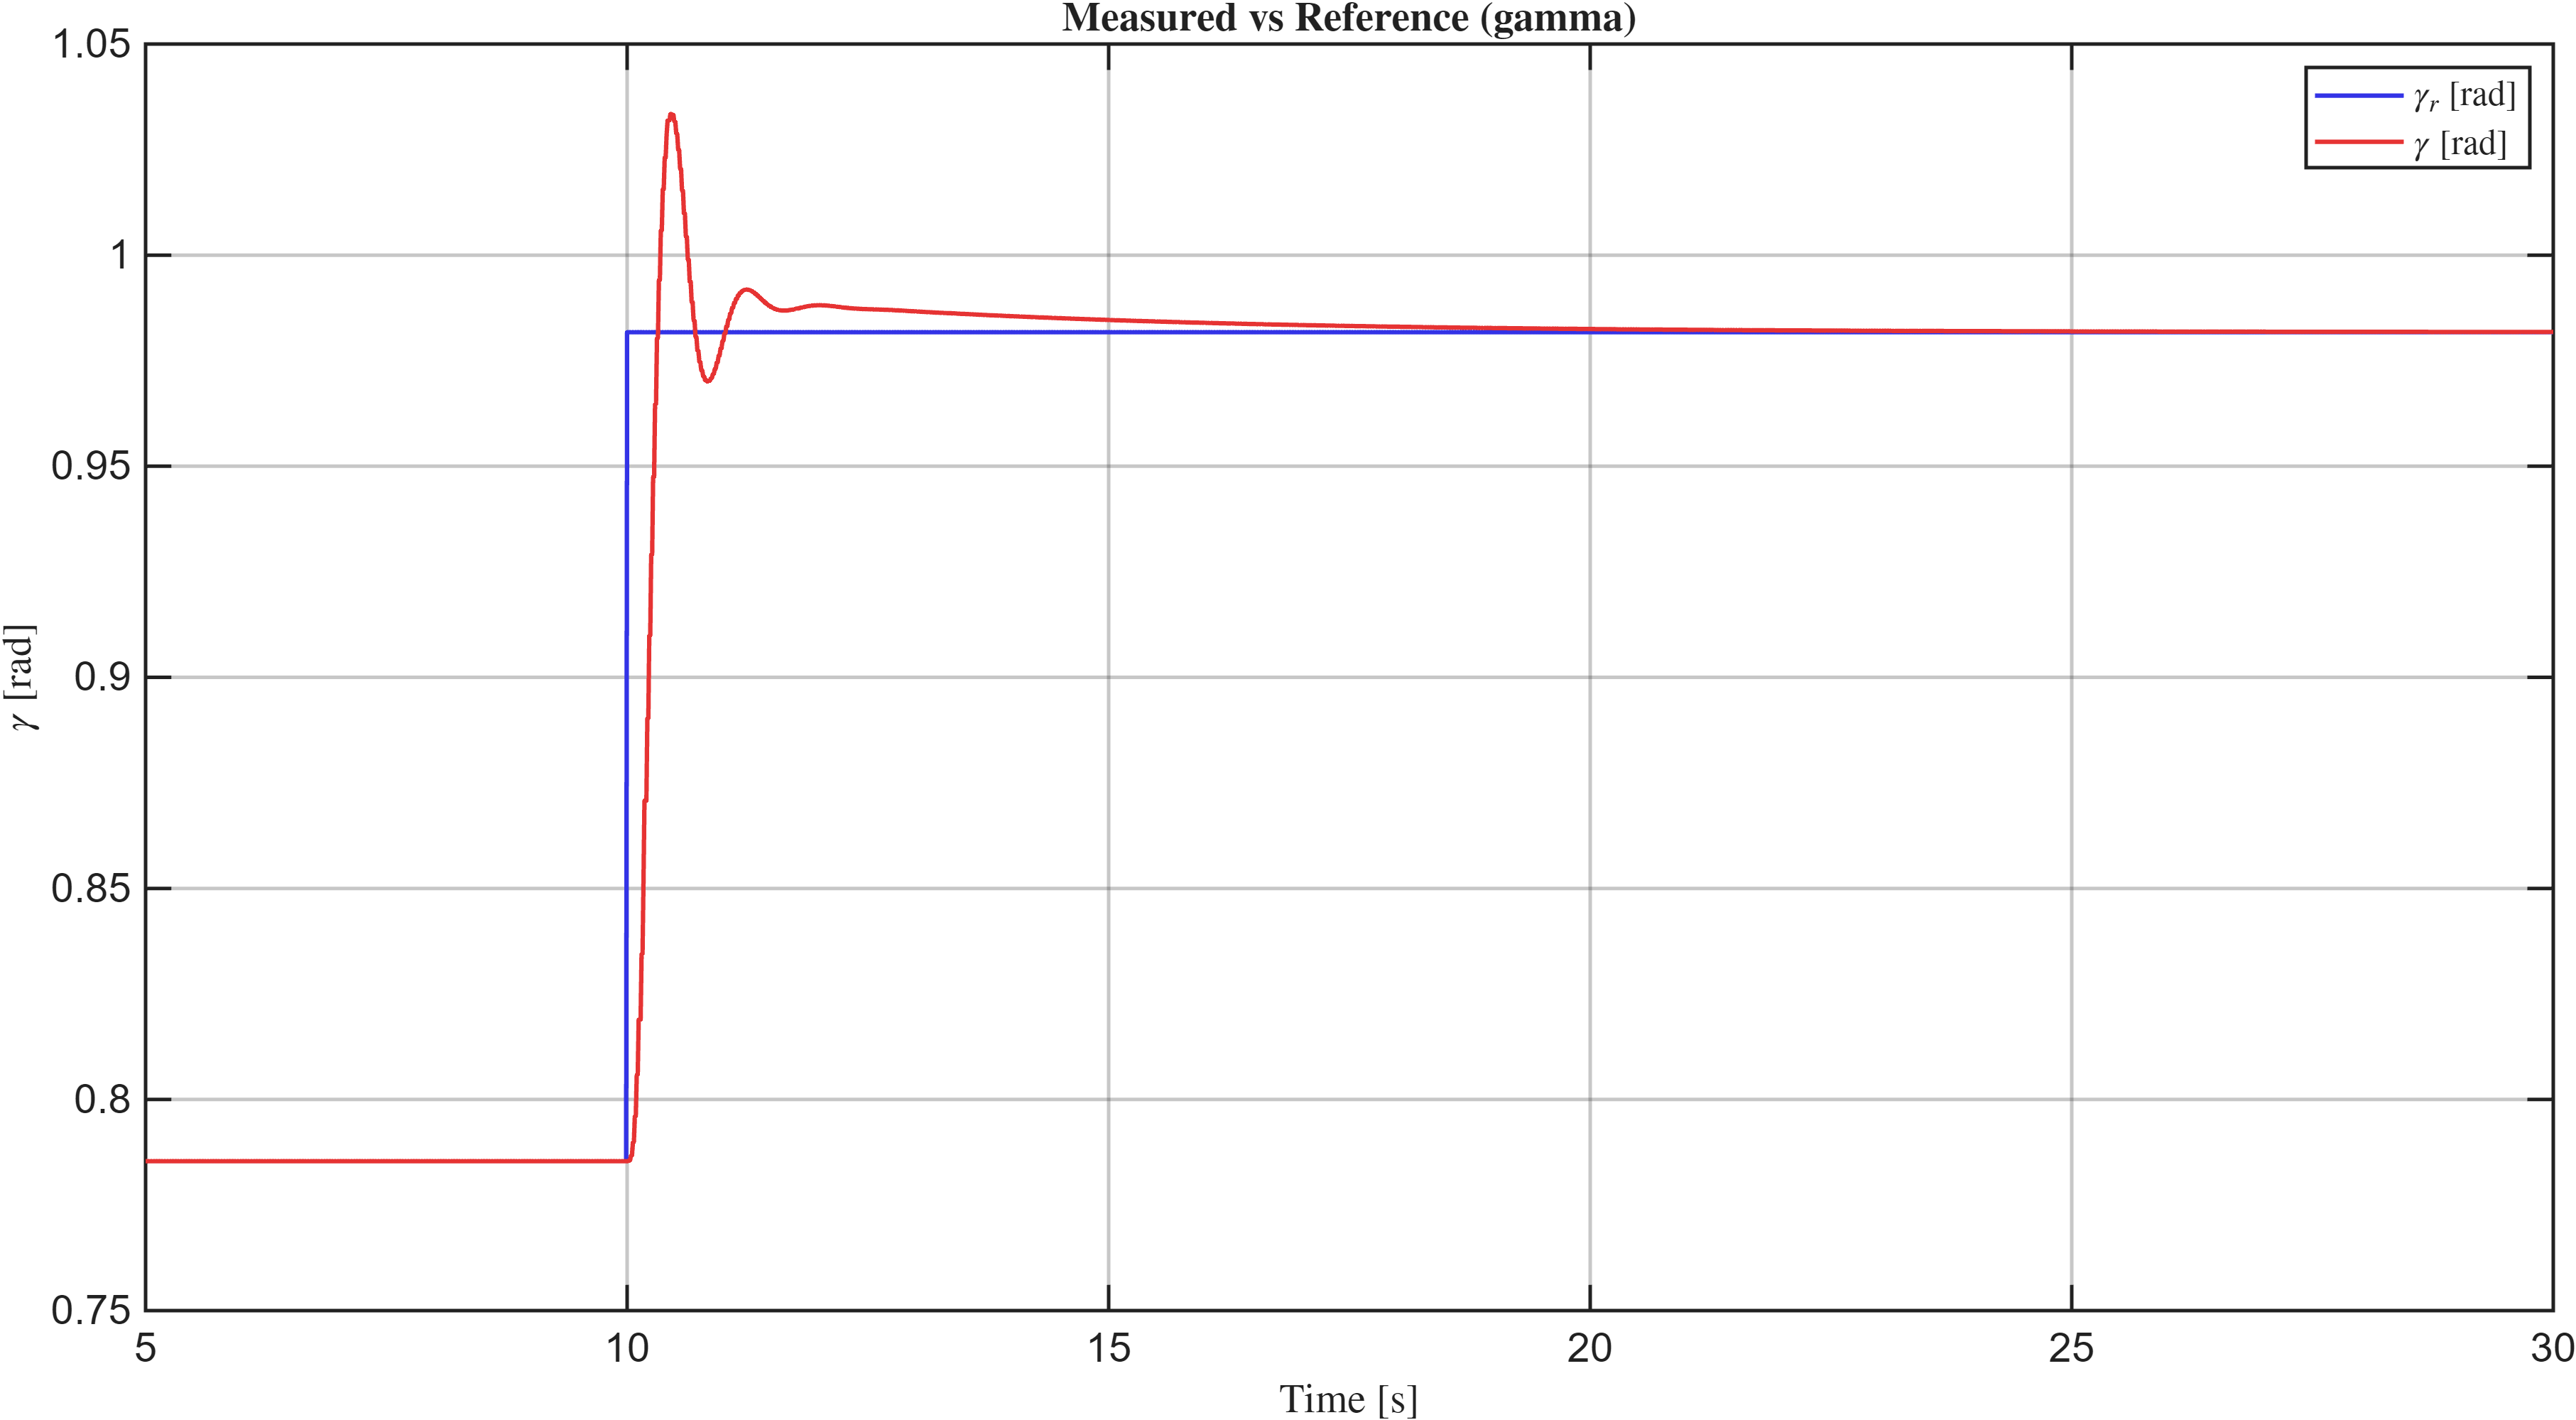
\includegraphics[width=0.75\textwidth]{img/step/gamma/pose-compare-gamma}
	\caption{پاسخ پله زاویه‌ای محور $\gamma$}
	\label{fig:results-gamma-step}
\end{figure}

ارزیابی کمّی عملکرد کنترل‌کننده‌ها برای هر سه درجه آزادی زاویه‌ای در جدول \ref{tab:results-angular-metrics} ارائه شده است. تحلیل این نتایج نشان می‌دهد که محورهای $\alpha$ و $\beta$ رفتار دینامیکی بسیار مشابهی دارند: زمان خیز در حدود $0.3$ ثانیه، زمان نشست نزدیک به $5$ ثانیه و فراجهش در محدوده‌ی $11$ تا $16$ درصد. خطای ماندگار این دو محور در مرتبه‌ی $10^{-8}$ رادیان و RMSE آن‌ها در حدود $0.0064$ رادیان است که بیان‌گر دقت بالای ردیابی در حالت ماندگار می‌باشد.

در مقابل، محور $\gamma$ با وجود زمان خیز طولانی‌تر ($0.71$ ثانیه)، زمان نشست به مراتب کوتاه‌تری (حدود $1.13$ ثانیه) و فراجهش کمتری ($5.26$ درصد) را به نمایش می‌گذارد. این امر نشان‌دهنده‌ی میرایی بیشتر و رفتار نوسانی ضعیف‌تر در این محور است. با این حال، خطای ماندگار این محور در مرتبه‌ی $10^{-5}$ رادیان و RMSE آن ($0.0154$ رادیان) حدوداً $2.5$ برابر مقادیر متناظر در محورهای $\alpha$ و $\beta$ است که عملکرد ضعیف‌تر آن را در ردگیری دقیق مسیر نشان می‌دهد.

به طور کلی، نتایج حاکی از آن است که علی‌رغم دستیابی به کنترل پایدار در هر سه راستای زاویه‌ای، مصالحه‌ای میان سرعت، میرایی و دقت رخ داده است. تلاش‌های صورت‌گرفته برای بهبود هم‌زمان این شاخص‌ها که مستلزم افزایش تلاش کنترلی بوده، به ناپایداری سامانه و شکست شبیه‌سازی منجر شده است. از این رو، با اذعان به محدودیت‌های ذاتی موجود، کنترل‌کننده‌های طراحی‌شده در این بخش می‌توانند به‌عنوان تضمینی برای حفظ پایداری دستگاه و امکان‌پذیری کنترل حرکت در صفحه مورد استفاده قرار گیرند.

\begin{table}[htbp]
	\centering
	\caption{شاخص‌های عملکرد پاسخ پله برای درجات آزادی زاویه‌ای}
	\label{tab:results-angular-metrics}
	\begin{tabular}{c c c c c c c}
		\toprule
		محور & زمان خیز & زمان نشست & فراجهش & زمان اوج & خطای ماندگار & RMSE \\
		\midrule
		$\alpha$ & \lr{0.3183} & \lr{5.2433} & \lr{11.068} & \lr{1.79} & \lr{$1.8926 \times 10^{-8}$} & \lr{0.0064164} \\
		$\beta$ & \lr{0.29999} & \lr{4.8722} & \lr{16.034} & \lr{1.12} & \lr{$6.3076 \times 10^{-8}$} & \lr{0.0064007} \\
		$\gamma$ & \lr{0.70657} & \lr{1.1254} & \lr{5.2594} & \lr{0.95} & \lr{$5.1615 \times 10^{-5}$} & \lr{0.015391} \\
		\bottomrule
	\end{tabular}
\end{table}

%====================================================
\subsection{رفتار تطبیقی کنترل‌کننده‌ی فازی-PID}
\label{subsec:results-fuzzy-adaptive}

مکانیزم تطبیق ضرایب در کنترل‌کننده‌ی فازی طراحی‌شده، مبتنی بر یک منطق واحد و نرمال‌شده است که از قواعد تشریح‌شده در بخش \ref{sec:method-control-design} پیروی می‌کند. از آن‌جا که هسته‌ی استنتاج فازی برای تمامی درجات آزادی یکسان است، الگوی کیفی تغییرات ضرایب در همه‌ی محورها رفتاری مشابه را به نمایش می‌گذارد و صرفاً مقیاس دامنه‌ی تغییرات، متناسب با بازه‌های بهره‌ی تعریف‌شده برای هر محور، متفاوت خواهد بود. در ادامه، ابتدا با بزرگ‌نمایی و تحلیل دقیق رفتار تطبیقی در یک محور نمونه ($X$)، منطق حاکم بر تغییرات ضرایب تشریح می‌شود و سپس الگوی مشابه در سایر محورها به صورت یکپارچه ارائه می‌گردد.

%----------------------------------------------------
\subsubsection{تحلیل رفتار تطبیقی: مطالعه‌ی موردی بر روی محور $X$}
\label{subsubsec:results-fuzzy-x}

برای تبیین نحوه‌ی عملکرد زمان‌بند بهره‌ی فازی، تغییرات ضرایب $K_p$، $K_i$ و $K_d$ در محور $X$ طی یک پاسخ پله، همراه با بزرگ‌نمایی یک اغتشاش ناگهانی، در شکل \ref{fig:results-fuzzy-x-gains} مورد بررسی قرار گرفته است. این تحلیل، نماینده‌ی رفتار سیستم در کلیه‌ی درجات آزادی است.

\begin{figure}[htbp]
	\centering
	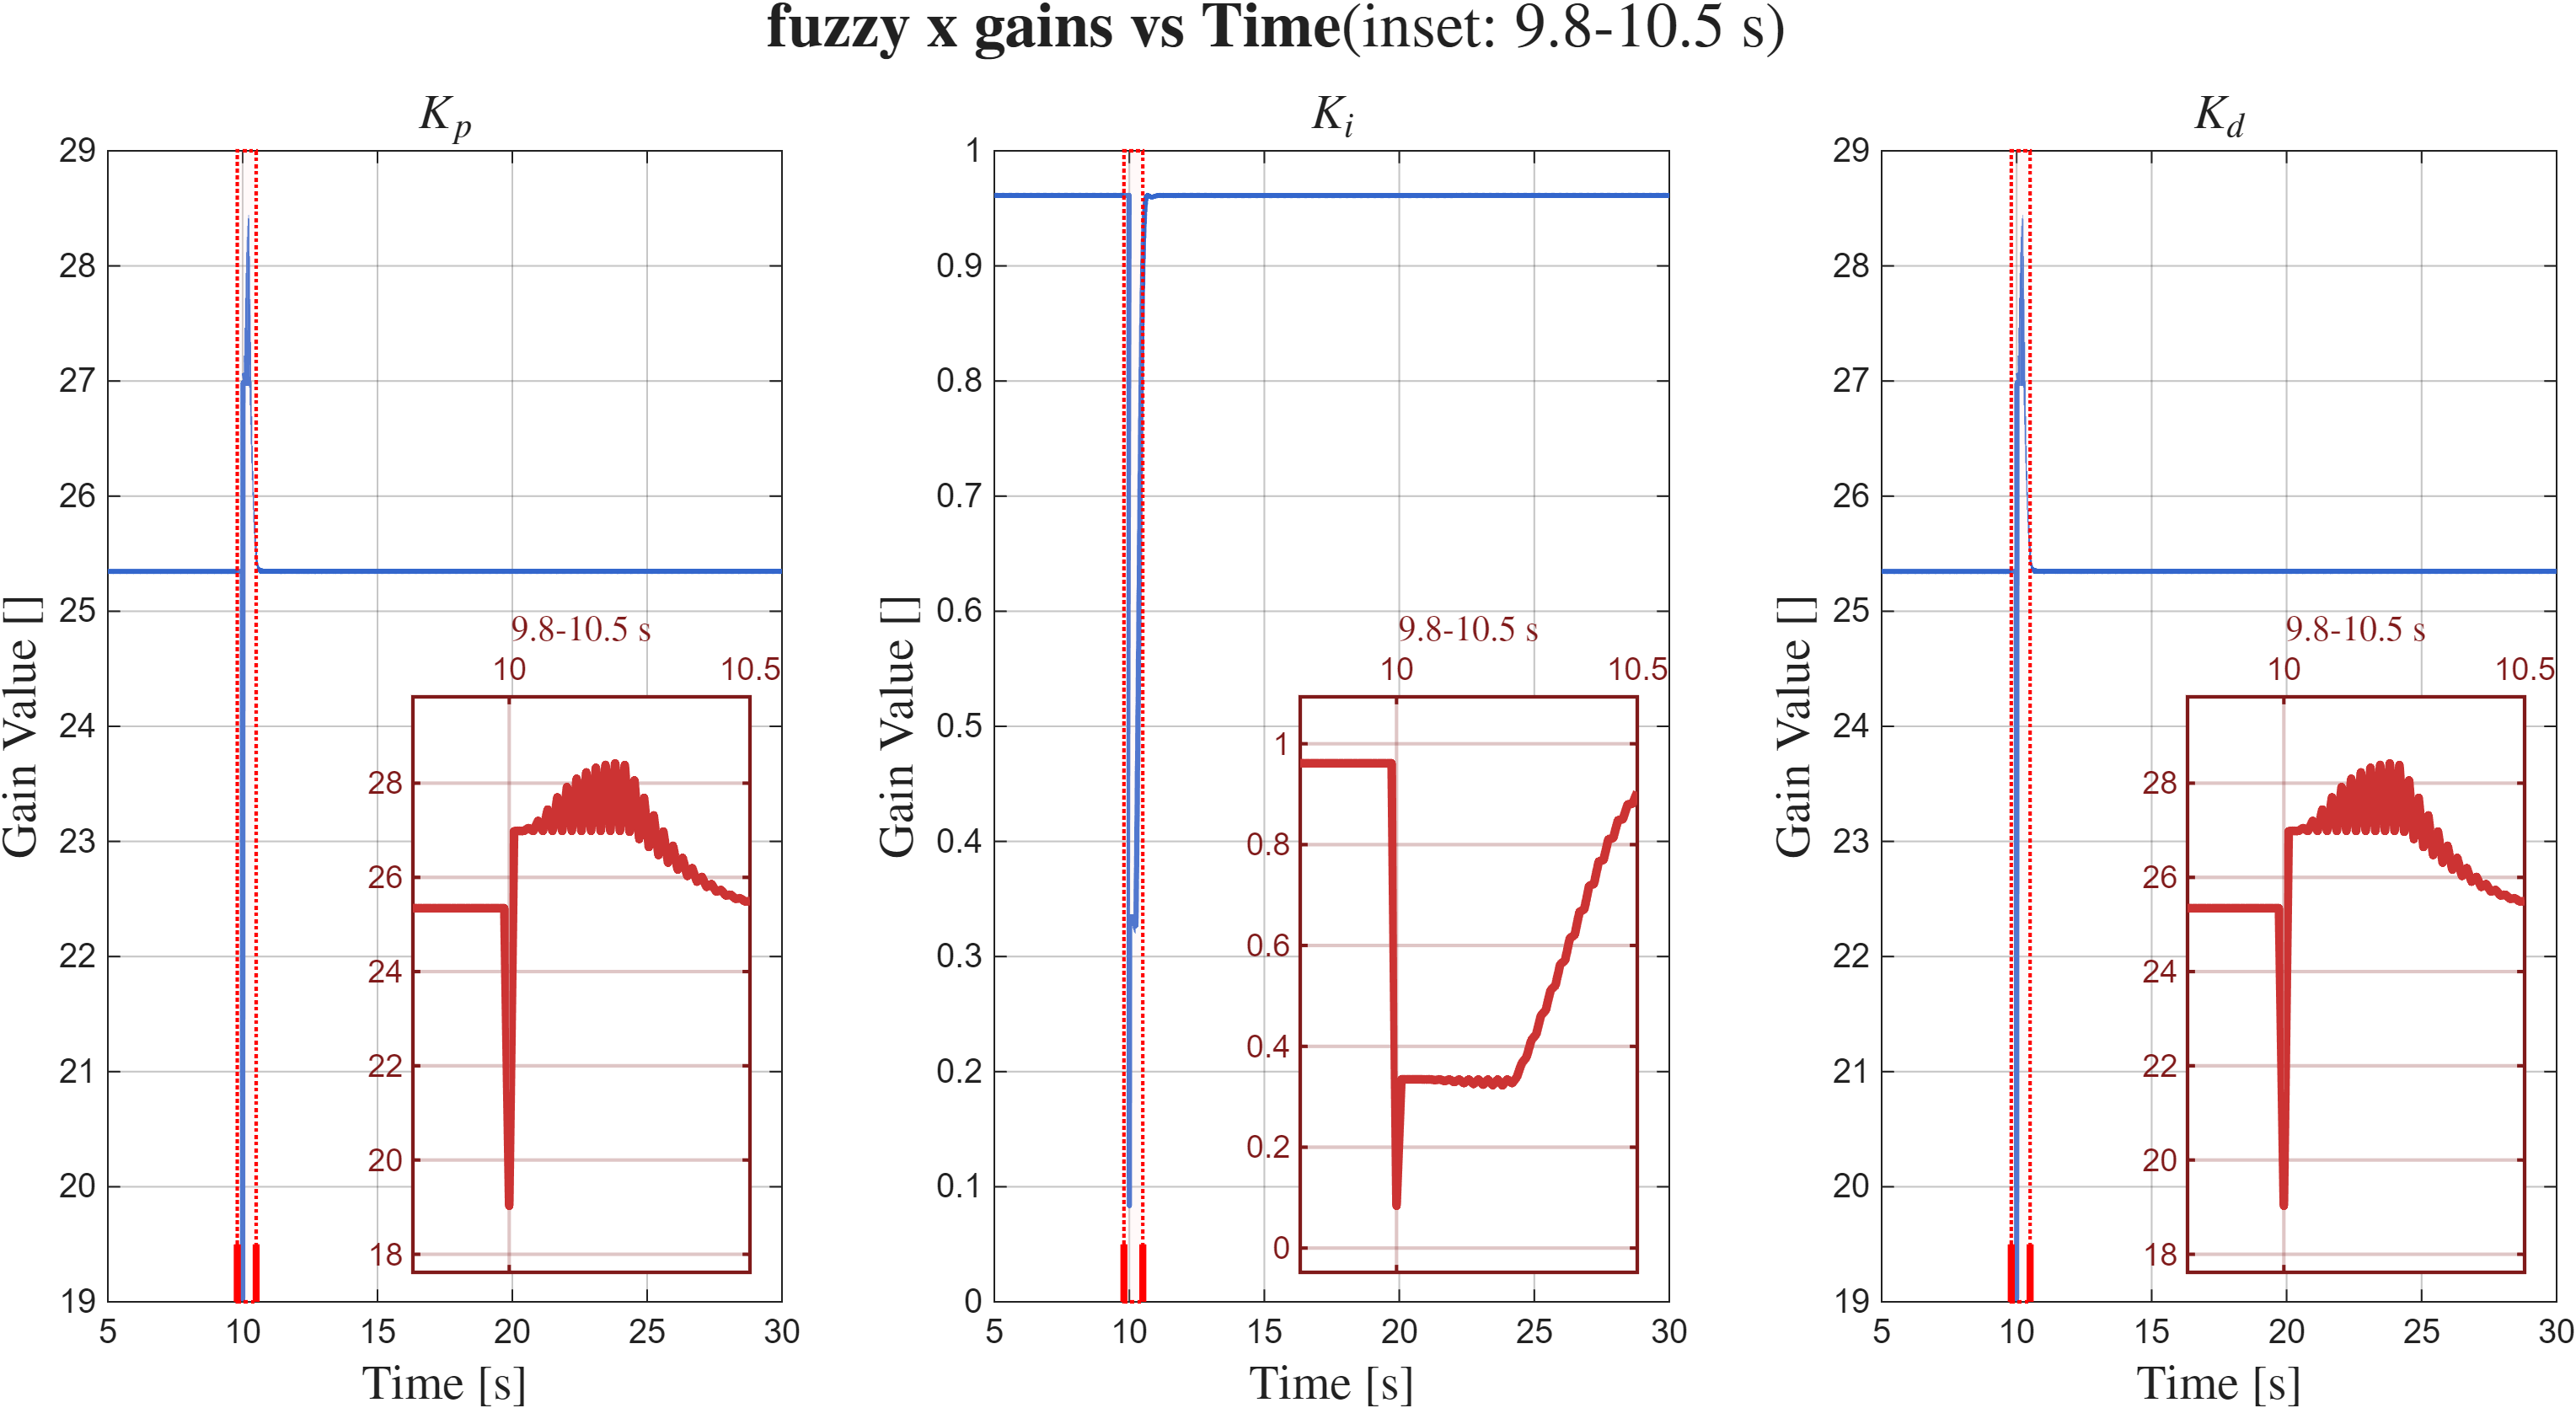
\includegraphics[width=0.85\textwidth]{img/step/x/fuzzy_x_gains_inset}
	\caption{تغییرات تطبیقی ضرایب کنترل‌کننده‌ی فازی-PID برای محور $X$ در زمان اعمال ورودی پله}
	\label{fig:results-fuzzy-x-gains}
\end{figure}

منطق تطبیق ضرایب بر پایه‌ی یک سیستم استنتاج فازی سوگنو با ۲۵ قاعده، دو ورودی نرمال‌شده‌ی خطا ($e_n$) و مشتق خطا ($de_n$) و سه خروجی ضرایب مقیاس‌دهنده‌ی $\alpha_p$، $\alpha_i$ و $\alpha_d$ عمل می‌کند. ضرایب واقعی کنترل‌کننده از حاصل‌ضرب این مقادیر در حداکثر بهره‌ی مجاز هر محور به دست می‌آید ($K_* = K_{*,\max} \times \alpha_*$). همان‌گونه که در شکل \ref{fig:results-fuzzy-x-gains} مشاهده می‌شود، در حالت ماندگار ($e_n \approx 0$، $de_n \approx 0$)، قاعده‌ی ۱۳ (\lr{$e_n$=Z, $de_n$=Z}) فعال بوده و ضرایب در مقادیر میانی خود (\lr{$\alpha_p$=M, $\alpha_i$=H, $\alpha_d$=M}) پایداری سیستم را تأمین می‌کنند.

با وارد شدن پله، مسیر حرکت روی سطوح فازی، توالی مشخصی از قواعد را فعال می‌کند که رفتار مشاهده‌شده را توجیه می‌نماید:
\begin{enumerate}
	\item \textbf{فروافتادگی (Dip):} در لحظه‌ی دور شدن ناگهانی خطا از صفر ($e_n$ بزرگ با علامت $de_n$ هم‌جهت)، قواعد ناحیه‌ی خطای بزرگ (مانند قاعده‌ی ۲۵) فعال می‌شوند که مقدار $\alpha_p$ را کم (L) و $\alpha_i$ را بسیار کم (VL) تعیین می‌کنند. این امر برای جلوگیری از اشباع انتگرال و کاهش حساسیت لحظه‌ای سیستم روی می‌دهد و منجر به افت ناگهانی $K_p$ و $K_i$ در نمودار می‌شود.
	\item \textbf{جهش جبرانی (Spike):} به محض معکوس شدن علامت مشتق خطا و بازگشت خطا به سمت صفر (در حالی که $e_n$ همچنان بزرگ است)، قواعدی مانند ۲۱ و ۱۶ فعال می‌شوند که $\alpha_p$ را خیلی زیاد (VH) یا زیاد (H) و $\alpha_d$ را زیاد (H) قرار می‌دهند. این افزایش ناگهانی بهره‌های تناسبی و مشتق، یک «پالس ترمزی» قوی برای متوقف کردن سریع خطا و جلوگیری از فراجهش ایجاد می‌کند که به‌صورت جهش در $K_p$ و $K_d$ نمایان می‌شود.
	\item \textbf{میرایی نوسانی:} با نزدیک شدن خطا به صفر و نوسان حول آن، سیستم بین قواعدی با خروجی‌های M و H جابه‌جا می‌شود. این کلیدزنی نرم، نوسانات میرا شونده‌ای را در $K_p$ و $K_d$ ایجاد می‌کند، در حالی که ضریب انتگرال $K_i$ به دلیل ماهیت فیلترشده‌اش، به آرامی به مقدار حالت ماندگار خود باز می‌گردد.
\end{enumerate}

این تحلیل نشان می‌دهد که چگونه مکانیزم فازی، با کاهش موقتی بهره‌ها هنگام فرار خطا و افزایش هوشمند آن‌ها هنگام بازگشت، به پاسخی سریع و در عین حال پایدار دست می‌یابد. این الگوی رفتاری، به دلیل اشتراک ساختار منطق فازی، در سایر محورها نیز دقیقاً تکرار می‌شود.

%----------------------------------------------------
\subsubsection{تغییرات ضرایب در درجات آزادی خطی}
\label{subsubsec:results-fuzzy-linear}

الگوی تطبیق تحلیل‌شده در محور $X$، در دو محور صفحه‌ای $Y$ و عمودی $Z$ نیز با انطباق کامل مشاهده می‌گردد. همان‌طور که در شکل \ref{fig:results-fuzzy-linear-gains} مشخص است، ساختار تغییرات ضرایب (افت اولیه، جهش جبرانی و میرایی نوسانی) در هر سه راستا یکسان بوده و تفاوت نمودارها تنها به دامنه‌ی نوسان و مقدار پایه‌ی ضرایب محدود می‌شود که آن نیز ناشی از تفاوت در $K_{*,\max}$ تنظیم شده برای غلبه بر دینامیک و اینرسی متفاوت در هر راستا است. این امر تأیید می‌کند که کنترل‌کننده‌ی فازی طراحی‌شده، مستقل از مقیاس، رفتار تطبیقی مقرر را ارائه می‌دهد.

\begin{figure}[htbp]
	\centering
	\subfloat[محور $X$]{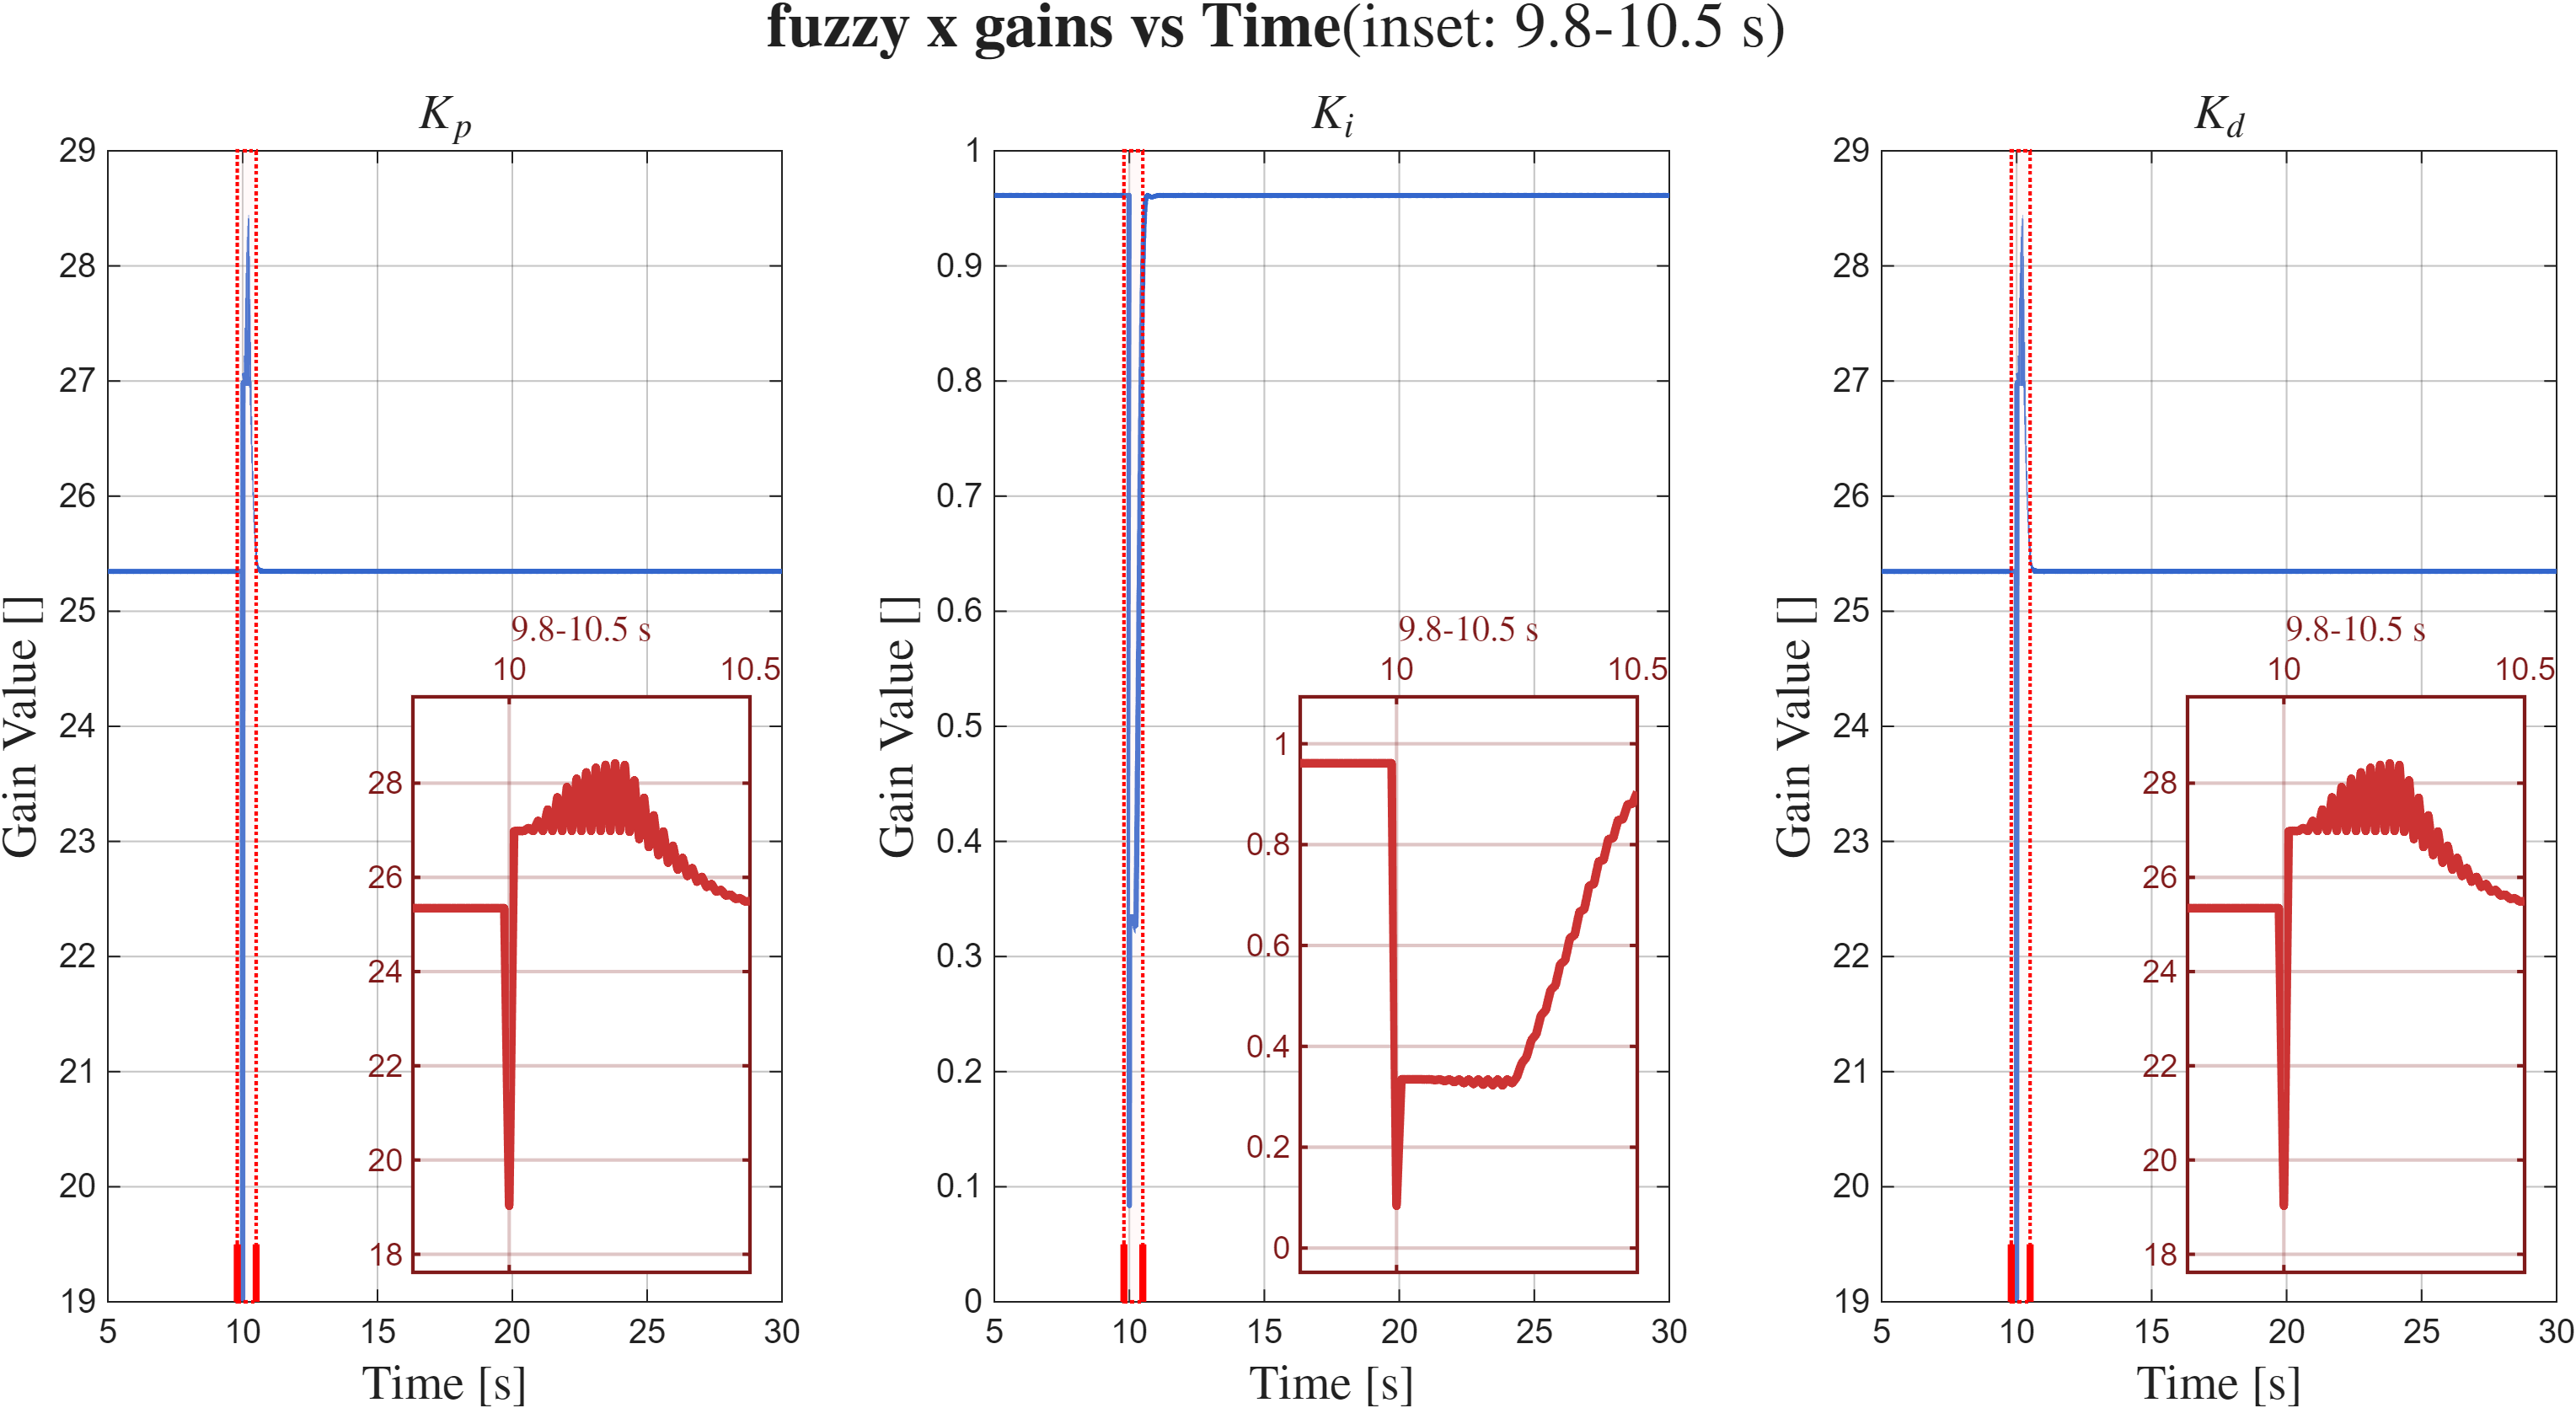
\includegraphics[width=0.48\textwidth]{img/step/x/fuzzy_x_gains_inset}}
	\hfill
	\subfloat[محور $Y$]{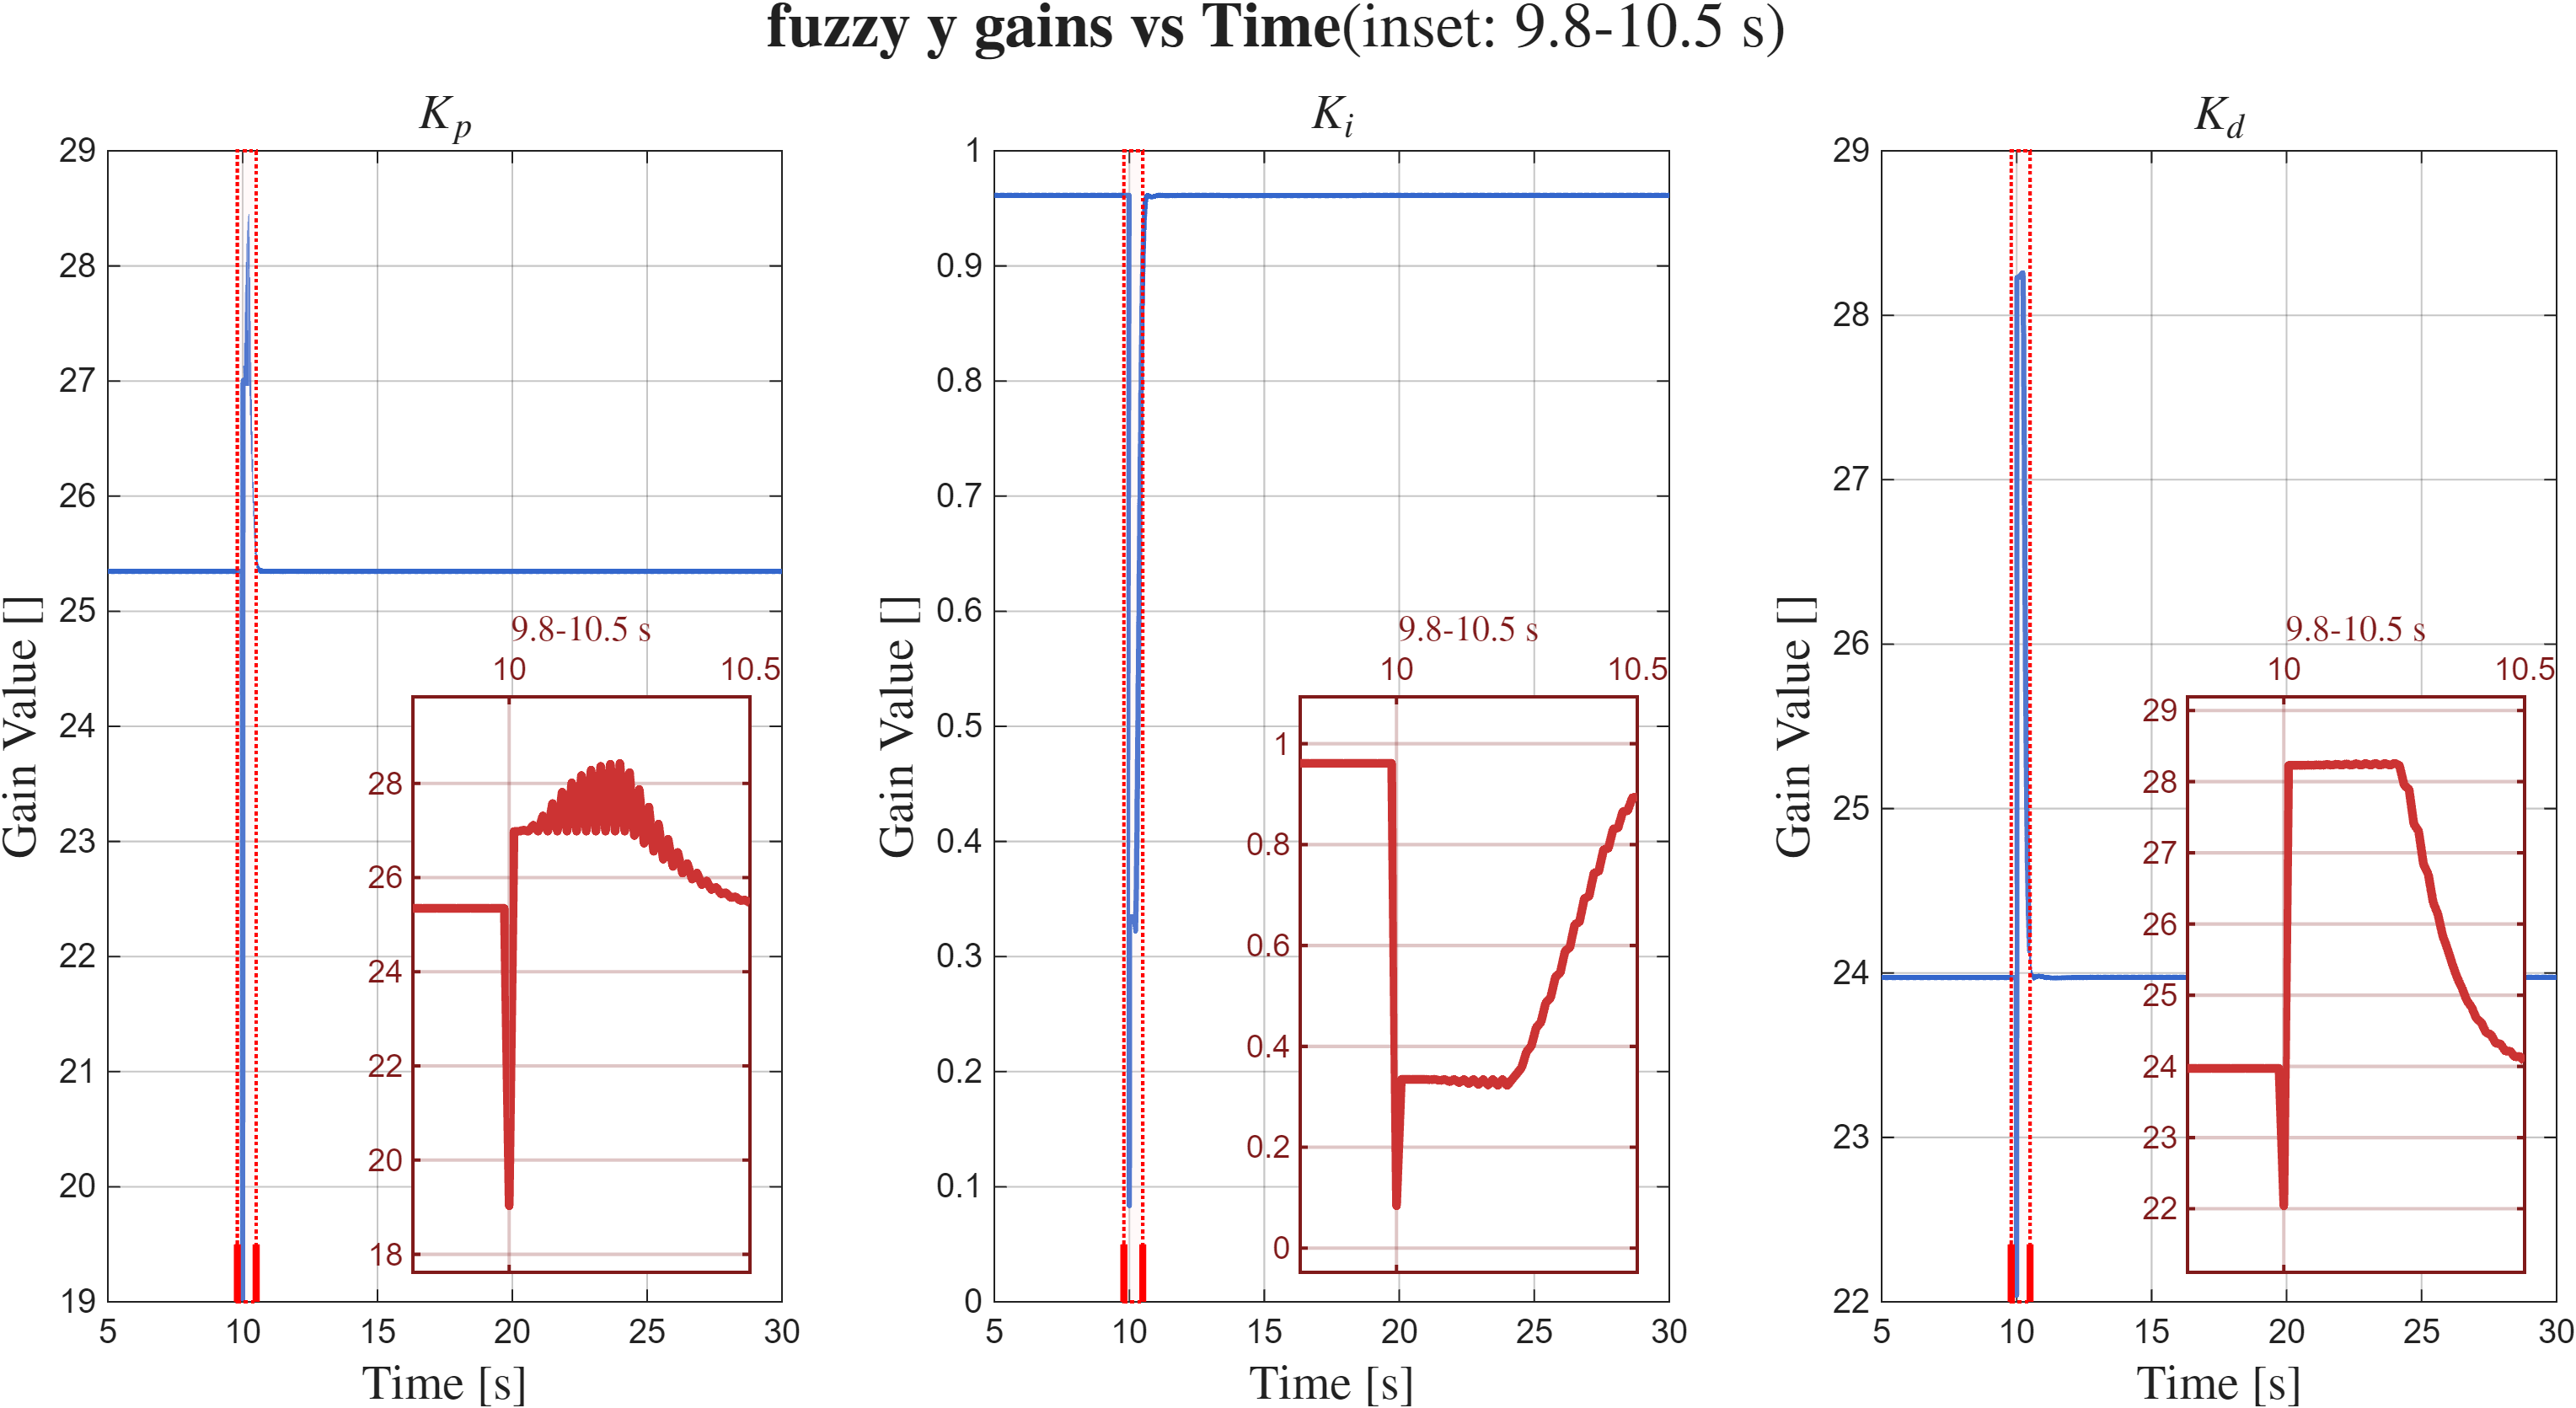
\includegraphics[width=0.48\textwidth]{img/step/y/fuzzy_y_gains_inset}}
	\\
	\subfloat[محور $Z$]{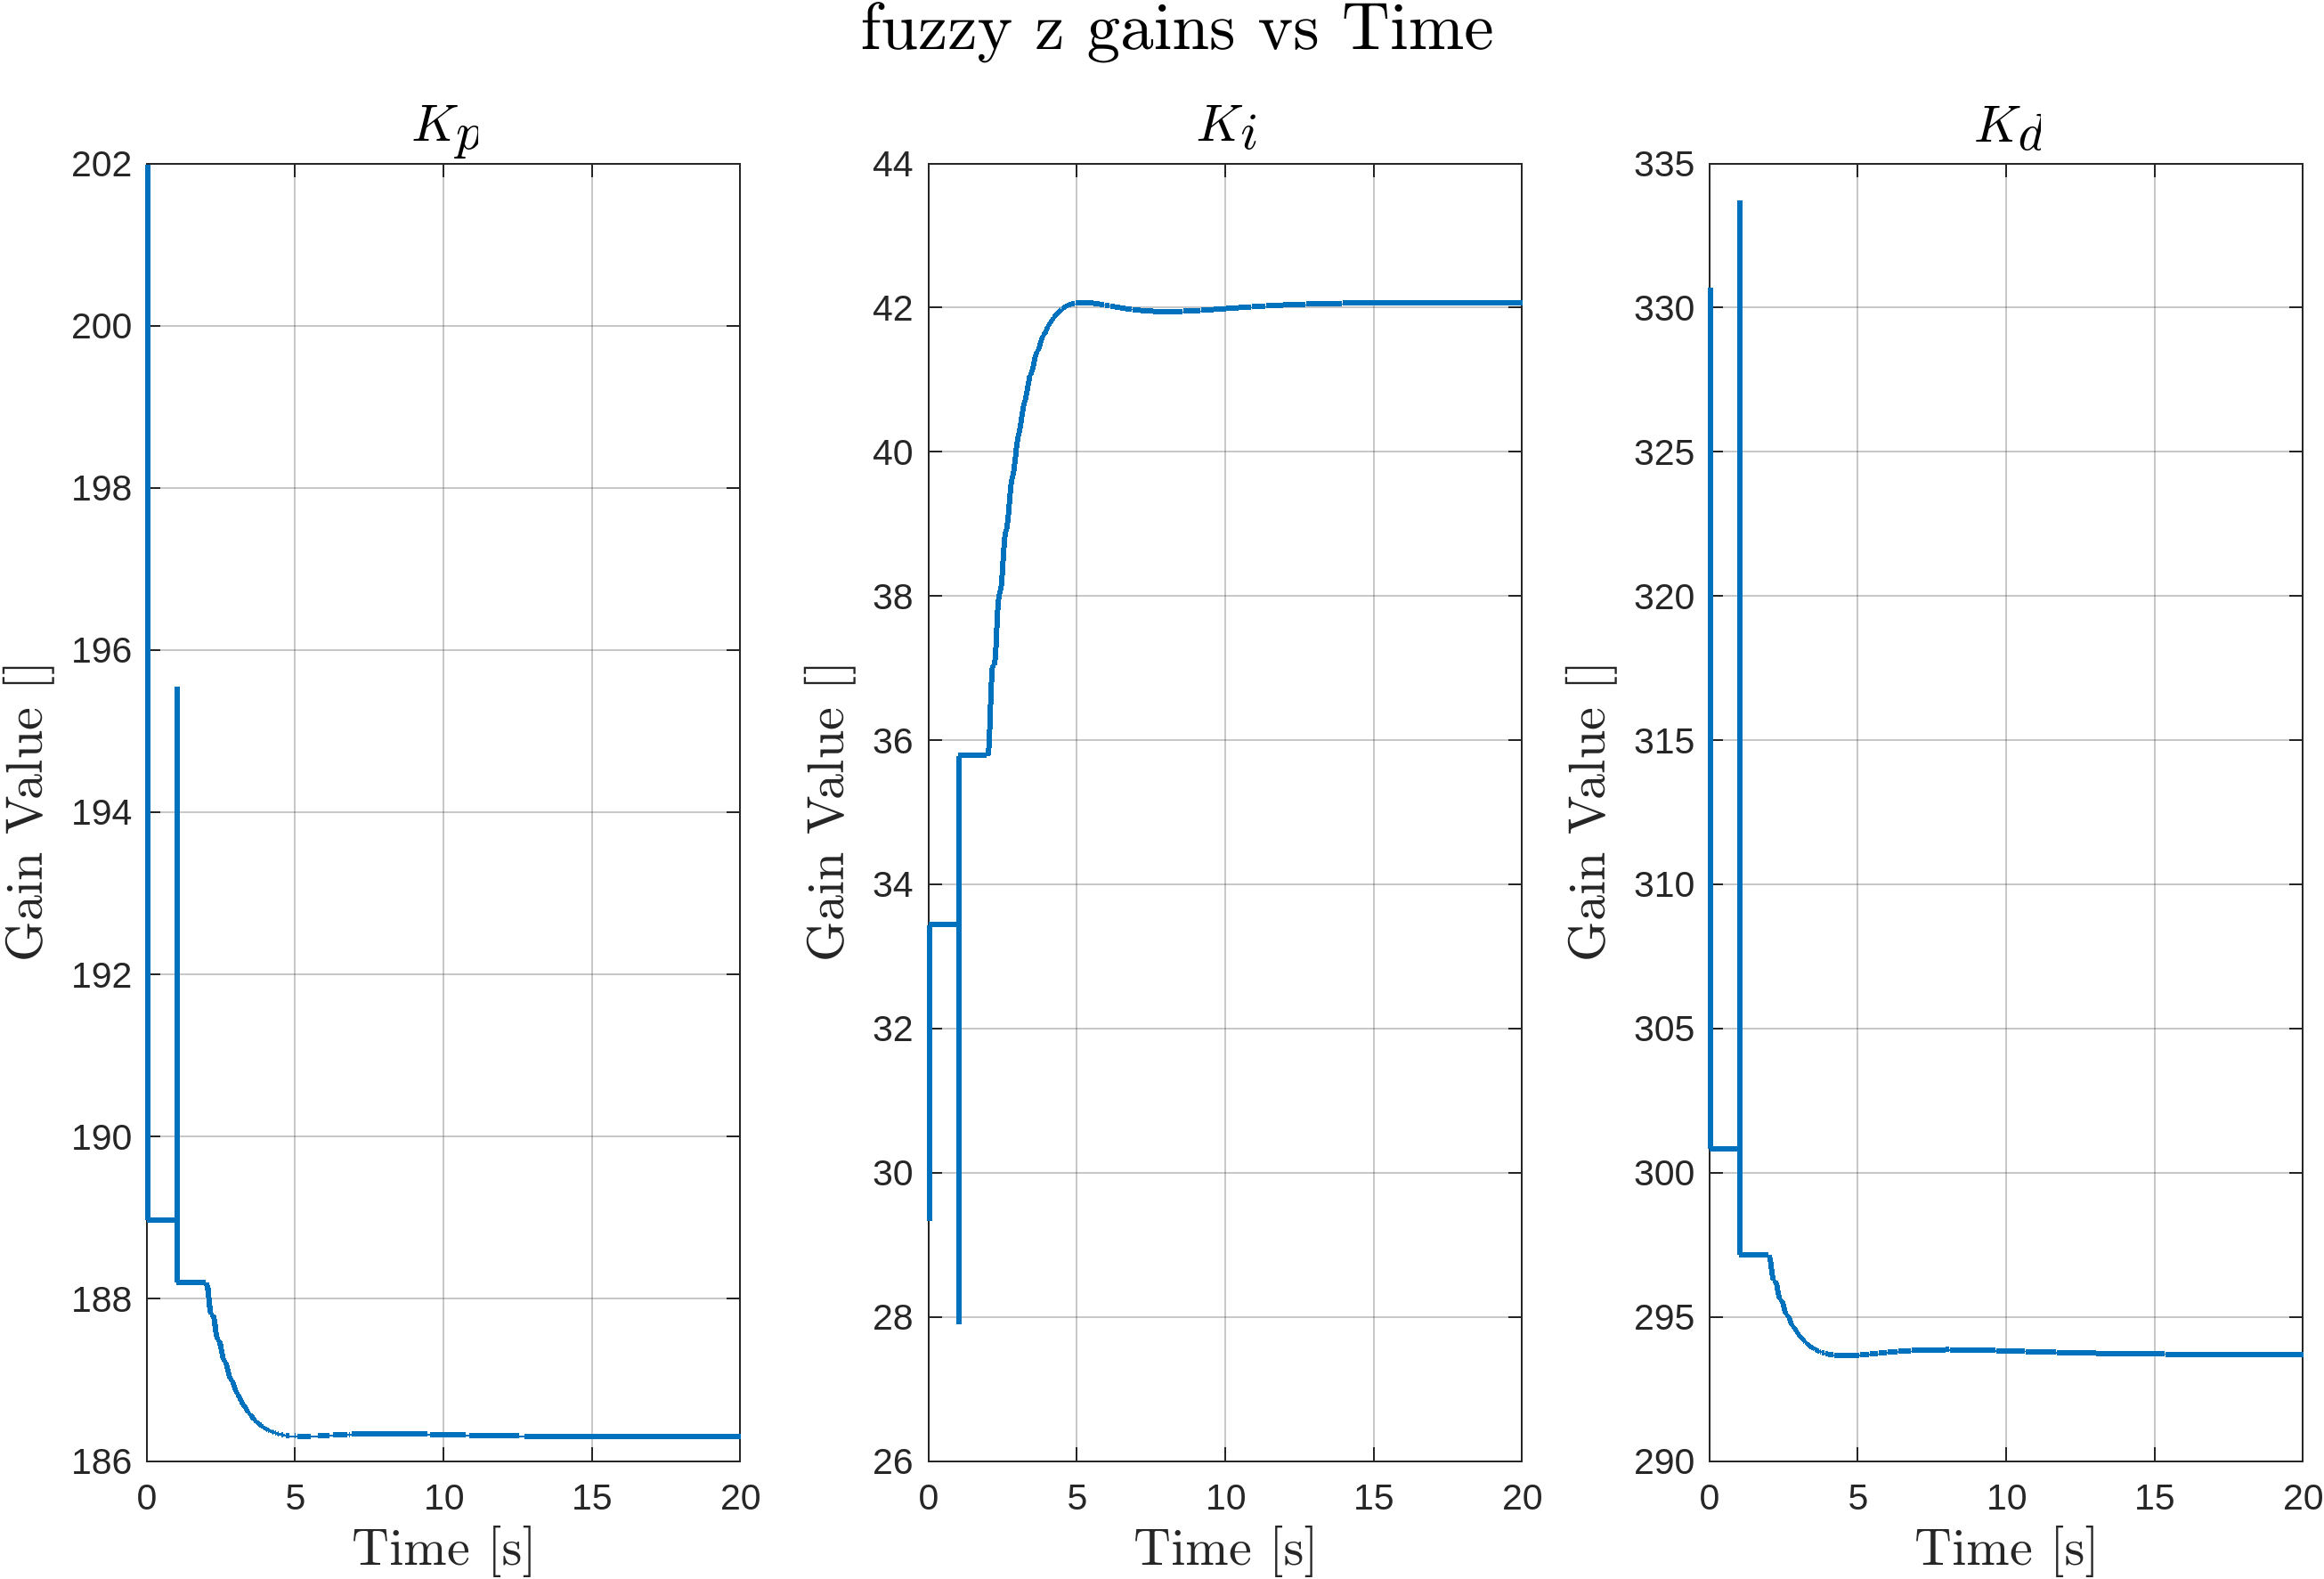
\includegraphics[width=0.65\textwidth]{img/step/z/fuzzy_z_gains}}
	\caption{تغییرات تطبیقی ضرایب کنترل‌کننده‌ی فازی-PID در درجات آزادی خطی}
	\label{fig:results-fuzzy-linear-gains}
\end{figure}

%----------------------------------------------------
\subsubsection{تغییرات ضرایب در درجات آزادی زاویه‌ای}
\label{subsubsec:results-fuzzy-angular}

منطق حاکم بر تغییرات ضرایب درجات آزادی زاویه‌ای $\alpha$، $\beta$ و $\gamma$ نیز به طور کامل از الگوی تشریح‌شده پیروی می‌کند. شکل \ref{fig:results-fuzzy-angular-gains} گواه آن است که توالی «افت - جهش - میرایی» به عنوان مشخصه‌ی ذاتی این زمان‌بند فازی، مستقل از نوع حرکت (خطی یا زاویه‌ای) در تمامی کانال‌ها برقرار است. این یکپارچگی در رفتار تطبیقی، ناشی از استفاده از یک سطح فازی نرمال‌شده‌ی مشترک است که با تغییر مقیاس ضرایب خروجی، خود را با دینامیک‌های گوناگون تطبیق می‌دهد.

\begin{figure}[htbp]
	\centering
	\subfloat[محور $\alpha$]{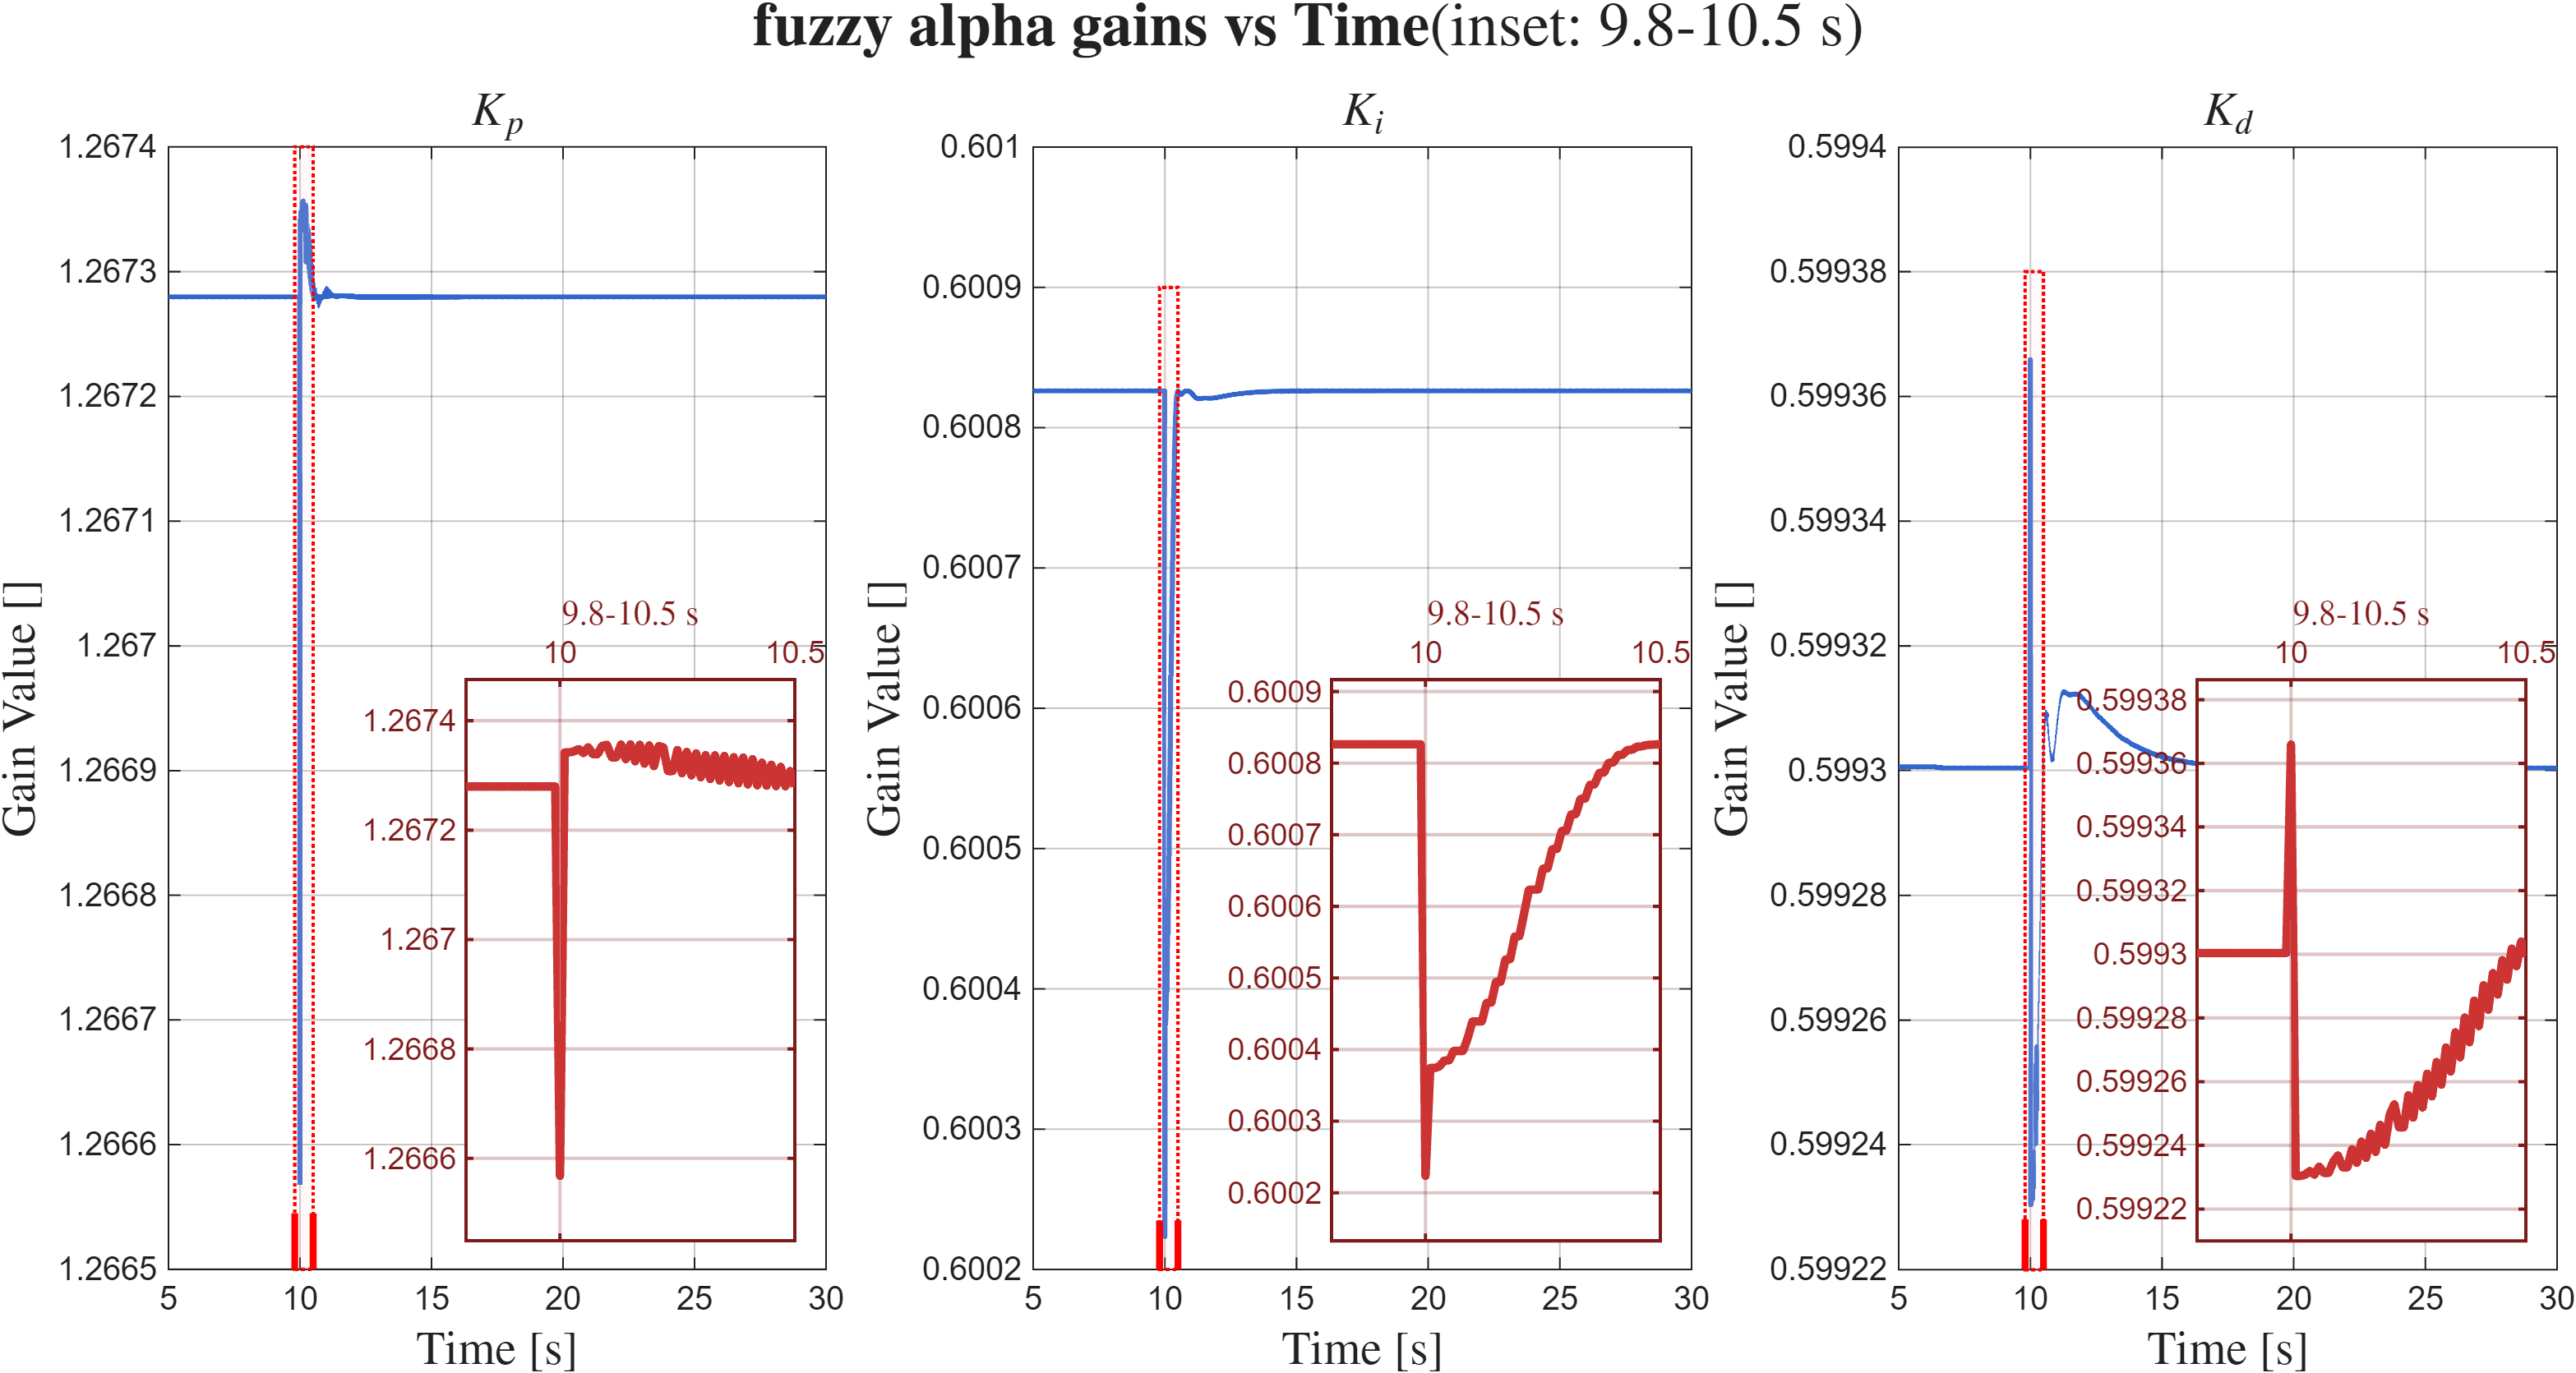
\includegraphics[width=0.48\textwidth]{img/step/alpha/fuzzy_alpha_gains_inset}}
	\hfill
	\subfloat[محور $\beta$]{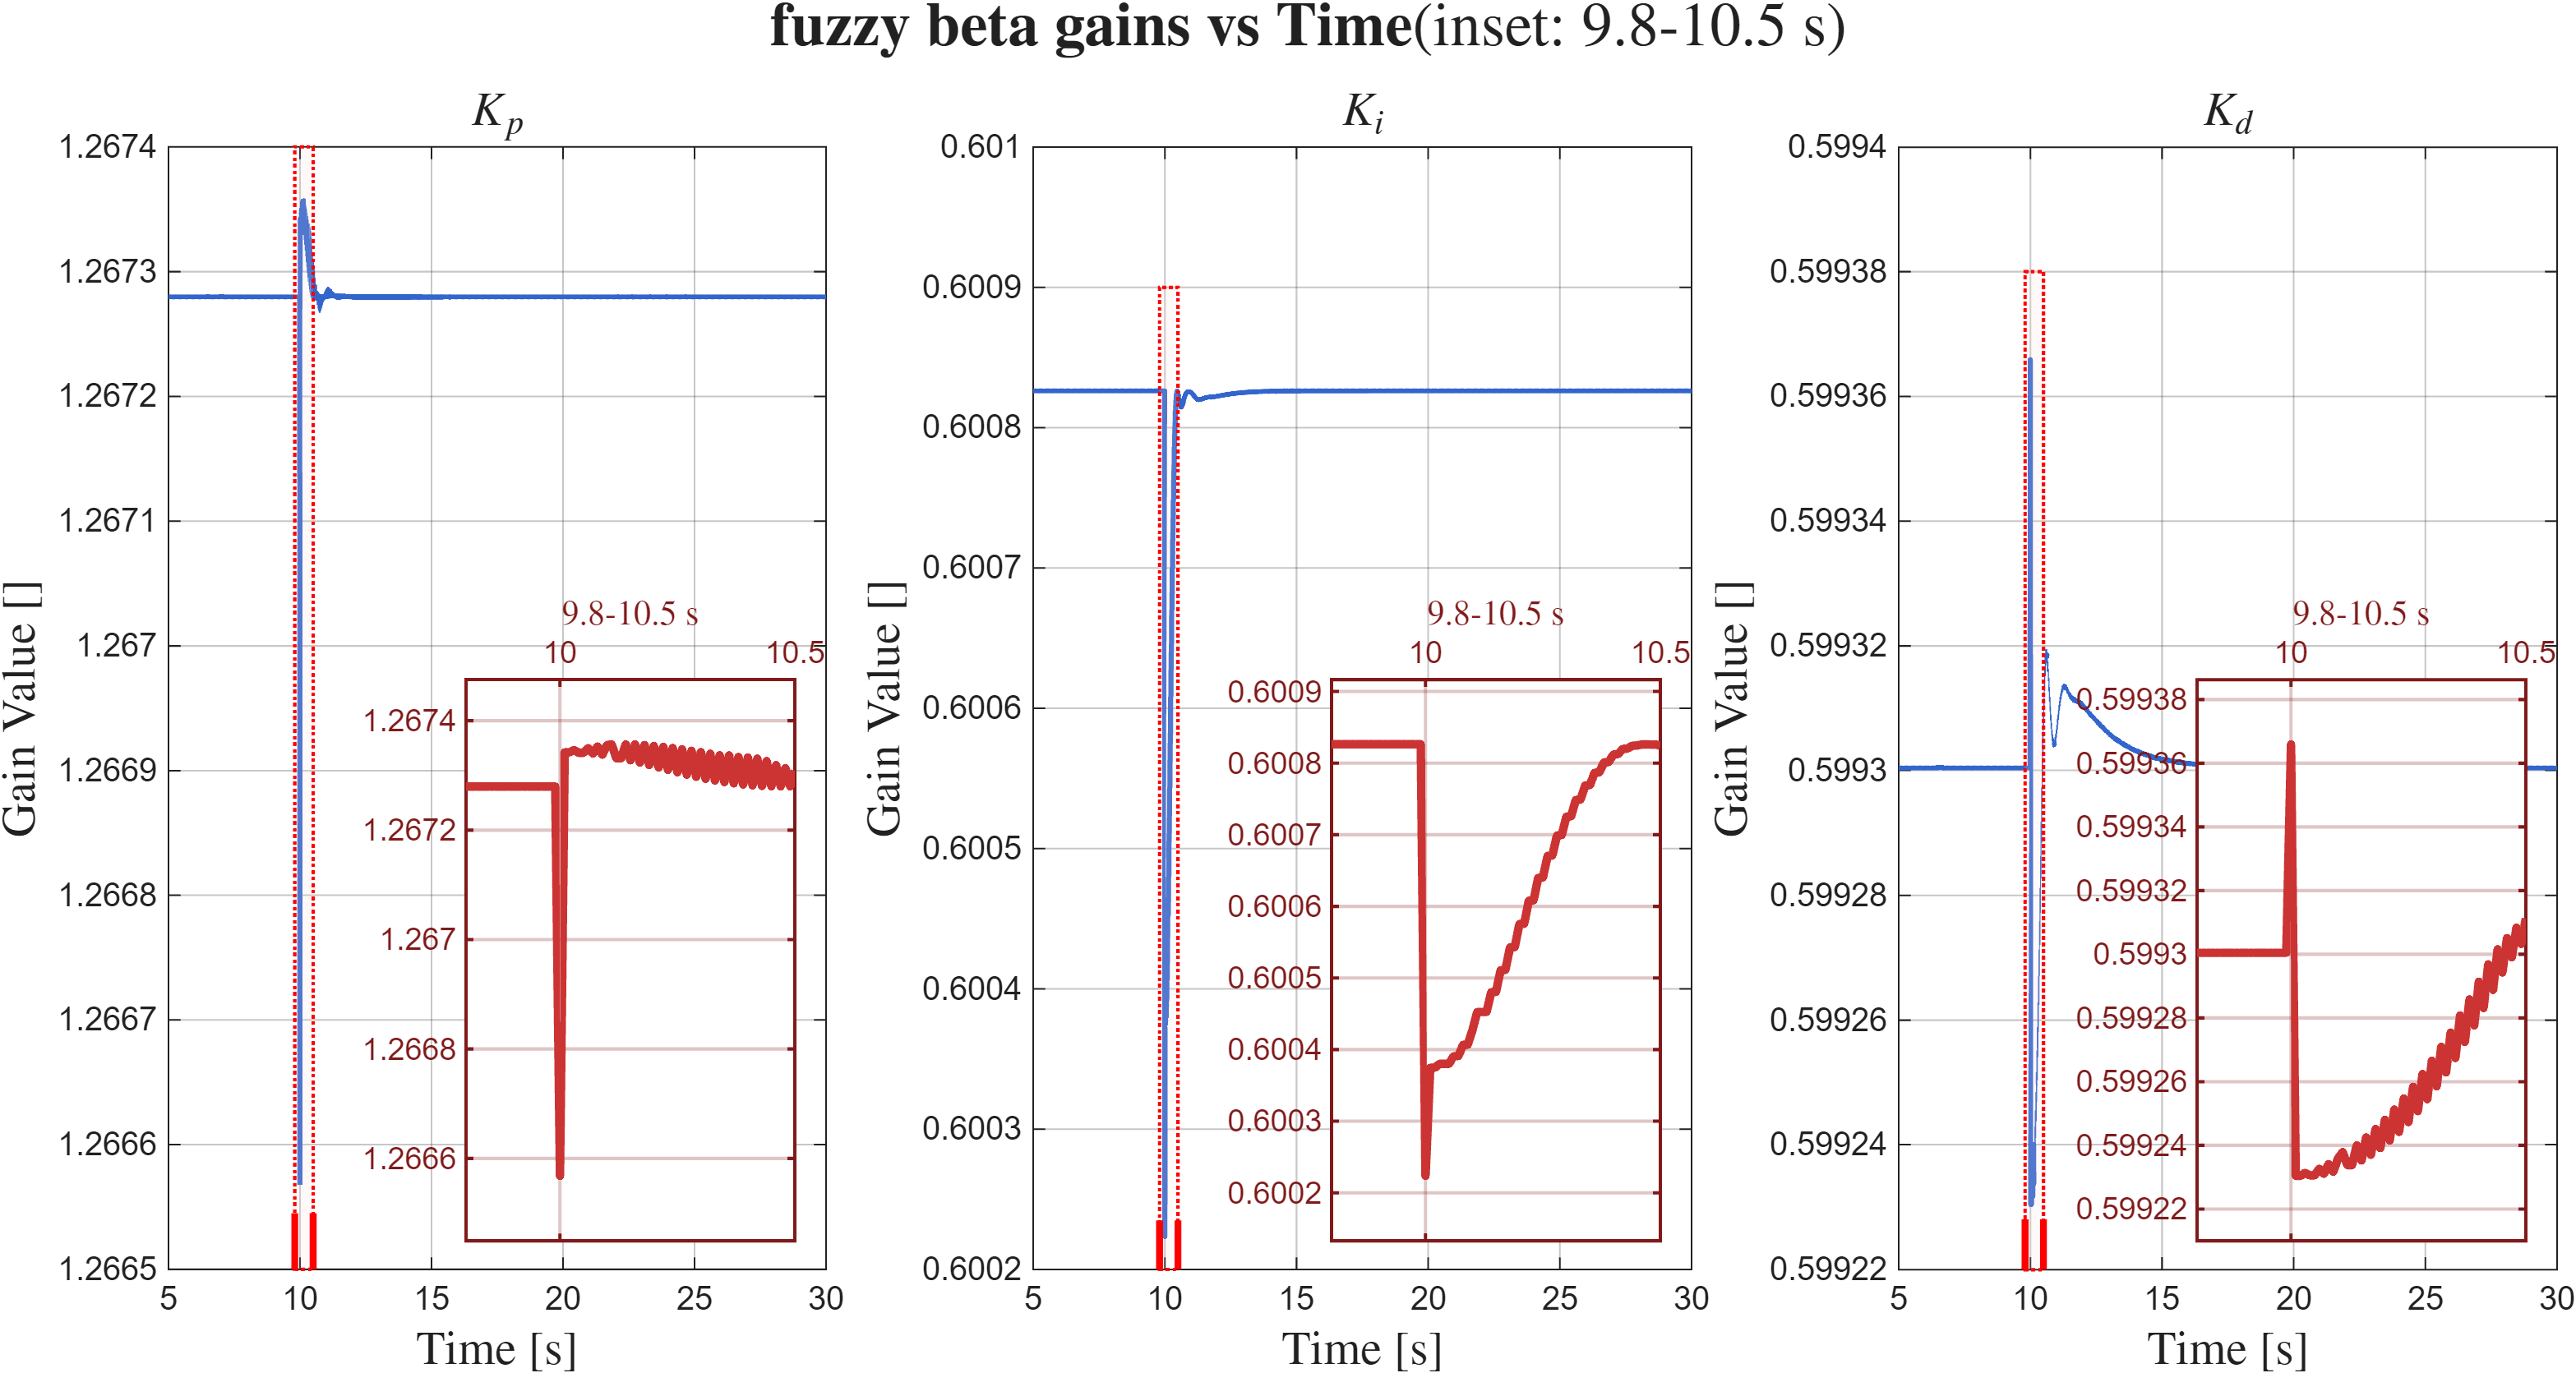
\includegraphics[width=0.48\textwidth]{img/step/beta/fuzzy_beta_gains_inset}}
	\\
	\subfloat[محور $\gamma$]{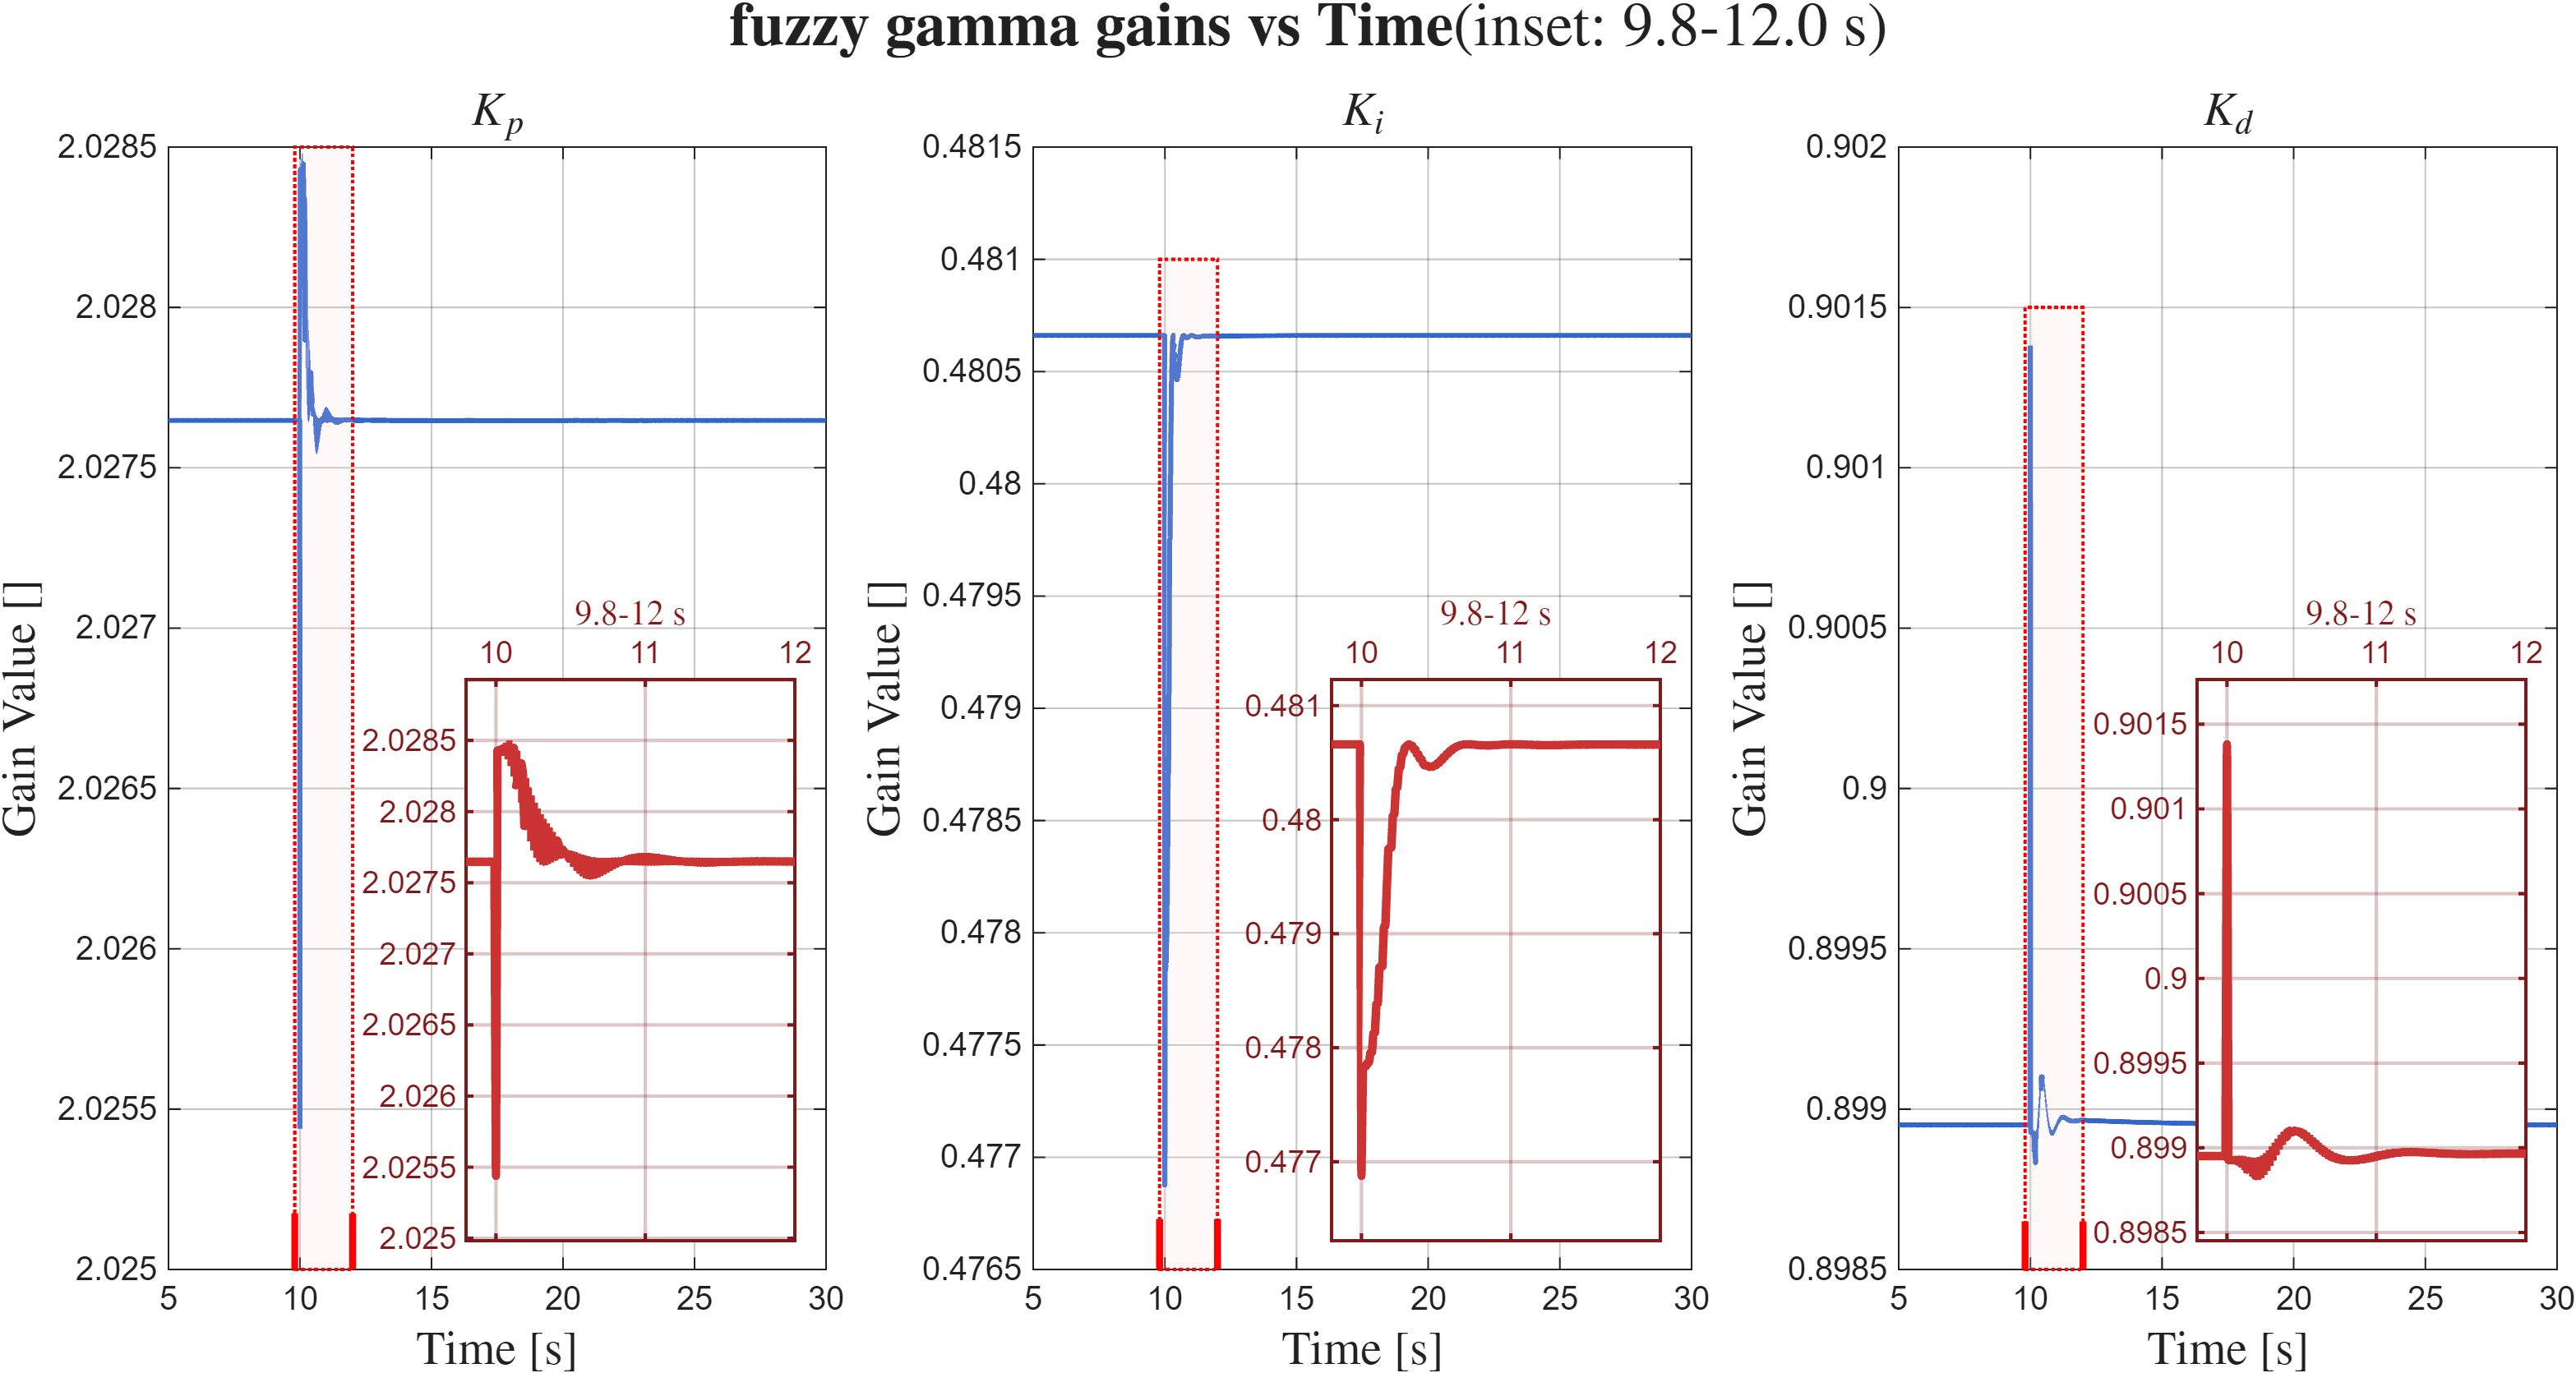
\includegraphics[width=0.65\textwidth]{img/step/gamma/fuzzy_gamma_gains_inset}}
	\caption{تغییرات تطبیقی ضرایب کنترل‌کننده‌ی فازی-PID در درجات آزادی زاویه‌ای}
	\label{fig:results-fuzzy-angular-gains}
\end{figure}

\subsection{مقایسه عملکرد کنترلر فازی-PID با کنترلر PID کلاسیک}
\label{subsec:results-comparison}

به منظور ارزیابی کمّی مزیت کنترلر فازی-PID پیشنهادی نسبت به یک کنترلر با ساختار مشابه اما فاقد مکانیزم تطبیق بهره، یک کنترلر PID کلاسیک با ضرایب ثابت به عنوان خط پایه (\lr{Baseline}) پیاده‌سازی و تحت شرایط یکسان آزموده شد. برای آنکه مقایسه صرفاً بازتاب‌دهنده‌ی تأثیر منطق فازی باشد و نه حاصل تفاوت در بهینه‌سازی جداگانه‌ی ضرایب، بهره‌های کنترلر کلاسیک بر مقادیر میانی (\lr{mid‑range}) همان محدوده‌ای تنظیم گردید که کنترلر فازی در حالت ماندگار حول آن عمل می‌کند. بدین ترتیب، هر دو کنترلر از یک خانواده‌ی بهره‌ی پایه بهره می‌برند و تفاوت مشاهده‌شده در پاسخ‌ها مستقیماً به توانایی سیستم فازی در تنظیم لحظه‌ای این بهره‌ها نسبت داده می‌شود.

هر دو کنترلر تحت شرایط کاملاً یکسان اجرا شدند: جابه‌جایی پله‌ای به اندازه‌ی $0.1$ متر در محور $X$، با اعمال محدودیت جریان $\pm9$ آمپر، محدودیت نرخ تغییرات جریان $80$ آمپر بر ثانیه، و در محیط فیزیکی یکسان شبیه‌ساز \lr{Gazebo}. نتایج کمّی این آزمون در جدول \ref{tab:controller_comparison_comprehensive} ارائه شده است.

\begin{table}[htbp]
	\centering
	\caption{مقایسه جامع عملکرد کنترلرها در پاسخ پله محور $X$}
	\label{tab:controller_comparison_comprehensive}
	\begin{tabular}{lccc}
		\toprule
		معیار & کنترلر فازی-PID & کنترلر PID کلاسیک & بهبود \\
		\midrule
		زمان خیز (\lr{$10\%$} تا \lr{$90\%$}) [s] & \lr{0.3600} & \lr{0.4000} & \textcolor{green!50!black}{\lr{$10.0\%$}} \\
		زمان اوج [s] & \lr{5.820} & \lr{5.900} & \textcolor{green!50!black}{\lr{$1.4\%$}} \\
		زمان نشست (\lr{$2\%$}) [s] & \lr{10.620} & \lr{11.060} & \textcolor{green!50!black}{\lr{$4.0\%$}} \\
		فراجهش [\%] & \lr{1.491} & \lr{2.615} & \textcolor{green!50!black}{\lr{$43.0\%$}} \\
		خطای حالت ماندگار [m] & \lr{0.000260} & \lr{0.000644} & \textcolor{green!50!black}{\lr{$59.7\%$}} \\
		بیشینه خطای مطلق [m] & \lr{0.1000} & \lr{0.1000} & \lr{$0.0\%$} \\
		RMSE [m] & \lr{0.0095} & \lr{0.0099} & \textcolor{green!50!black}{\lr{$4.1\%$}} \\
		MAE [m] & \lr{0.0015} & \lr{0.0020} & \textcolor{green!50!black}{\lr{$26.0\%$}} \\
		\bottomrule
	\end{tabular}
\end{table}

همان‌طور که از جدول \ref{tab:controller_comparison_comprehensive} استنتاج می‌شود، کنترلر فازی-PID در تمامی شاخص‌ها، به جز بیشینه خطای مطلق که در هر دو حالت یکسان باقی مانده است، عملکرد برتری را به ثبت رسانده است. کاهش قابل‌توجه در فراجهش ($43\%$) و خطای حالت ماندگار ($59.7\%$) نشان می‌دهد که مکانیزم تطبیقی فازی به‌طور مؤثری از خود فراجهشی و انباشت خطای باقی‌مانده جلوگیری کرده است.

شکل \ref{fig:comparison_all} سه جنبه از مقایسه میان دو کنترلر را در یک نمای واحد گردآوری کرده است. شکل \ref{fig:step_comparison} پاسخ پله دو کنترلر را به صورت هم‌زمان نمایش می‌دهد. در این نمودار، هم‌گرایی سریع‌تر، فراجهش کمتر و نوسانات میراتر کنترلر فازی در مقایسه با PID کلاسیک کاملاً مشهود است. شکل \ref{fig:error_comparison} سیگنال خطا را در طول زمان مقایسه می‌کند و نشان می‌دهد که کنترلر فازی خطا را با سرعت بیشتری به سمت صفر هدایت کرده و دامنه‌ی نوسانات خطا را نیز محدودتر نگاه داشته است. رفتار متمایز کنترلر فازی-PID در نمودار تلاش کنترلی (شکل \ref{fig:effort_comparison}) نیز تحلیل‌پذیر است. کنترلر فازی در لحظات آغازین پله، یک جهش نیروی قوی‌تر اعمال می‌کند که ناشی از افزایش هوشمند بهره‌های تناسبی و مشتقی در فاز «جهش جبرانی» تحلیل‌شده در بخش \ref{subsubsec:results-fuzzy-x} است. این پالس نیروی اضافی، که همواره در محدوده‌ی مجاز عملگرها باقی می‌ماند، همان عاملی است که زمان خیز را کاهش داده و خطای ماندگار را سریع‌تر از بین می‌برد. در مقابل، کنترلر PID کلاسیک با بهره‌های ثابت خود قادر به تولید چنین واکنش تطبیقی و کنترل‌شده‌ای نیست و در نتیجه، خطای ماندگار برای مدت طولانی‌تری در پاسخ حضور دارد.

\begin{figure}[htbp]
	\centering
	\subfloat[مقایسه پاسخ پله دو کنترلر در محور $X$]{
		\label{fig:step_comparison}
		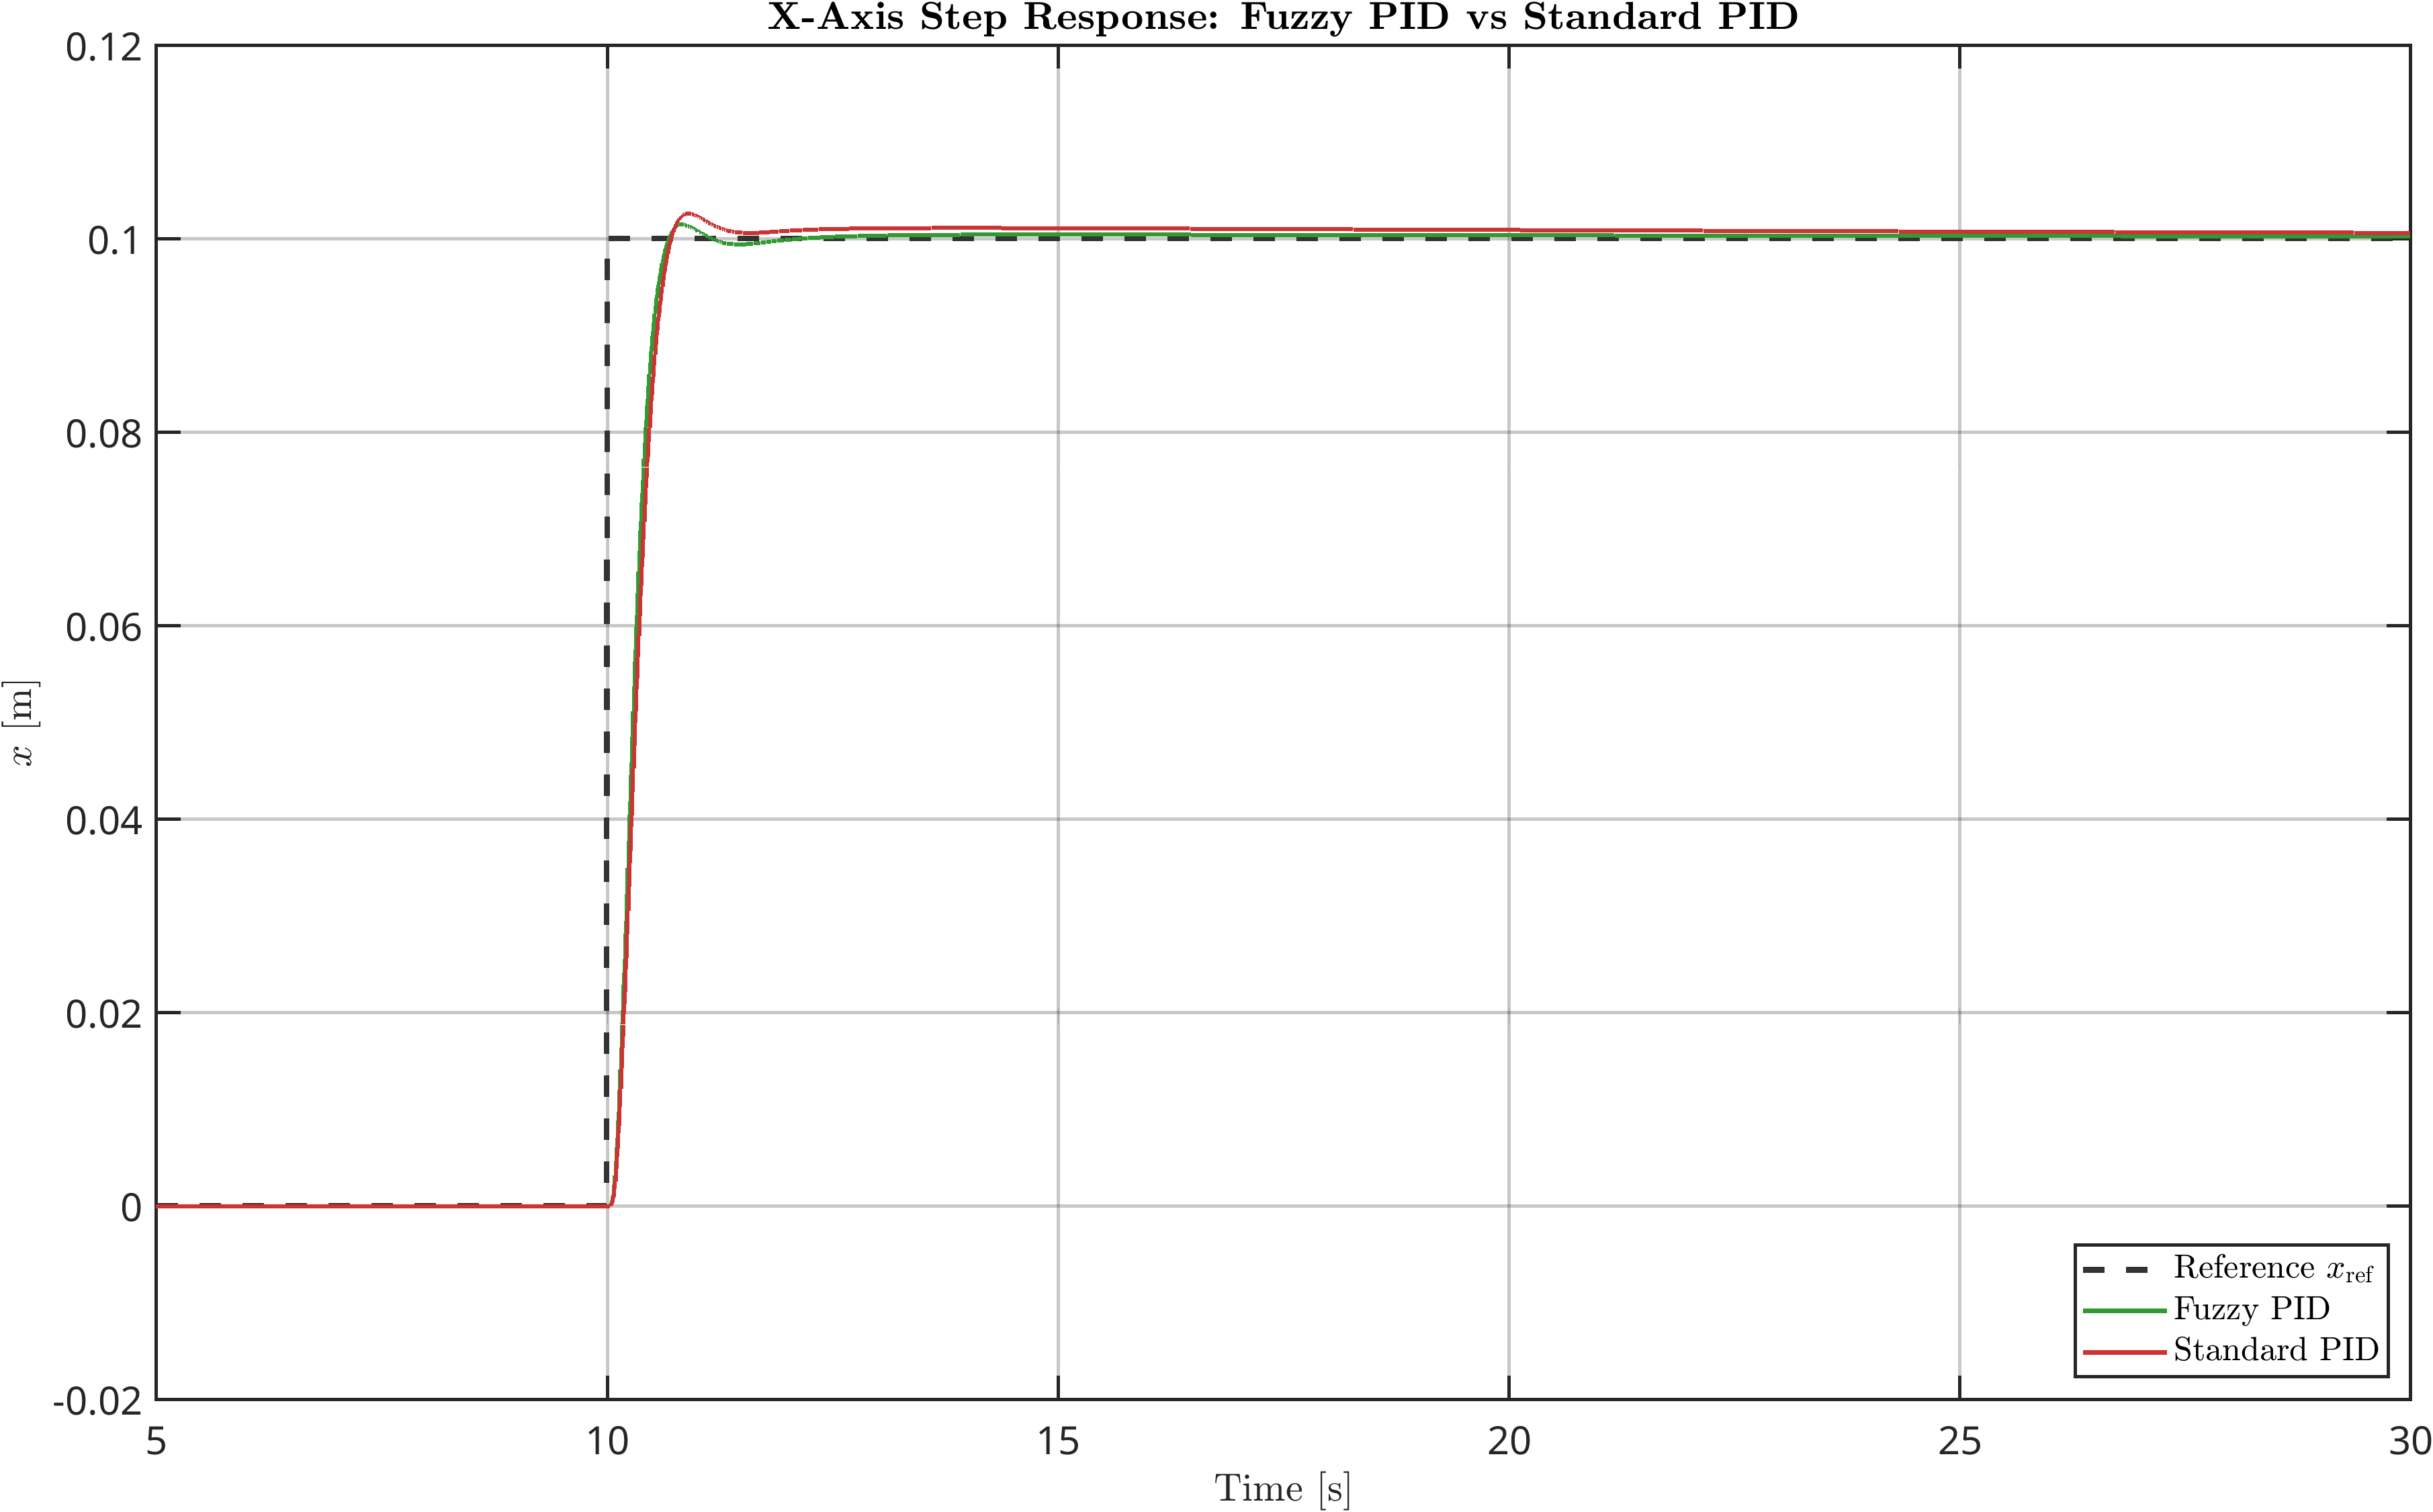
\includegraphics[width=0.48\textwidth]{img/step/x/controller-comparison-x-step}}
	\hfill
	\subfloat[مقایسه سیگنال خطا در طول زمان]{
		\label{fig:error_comparison}
		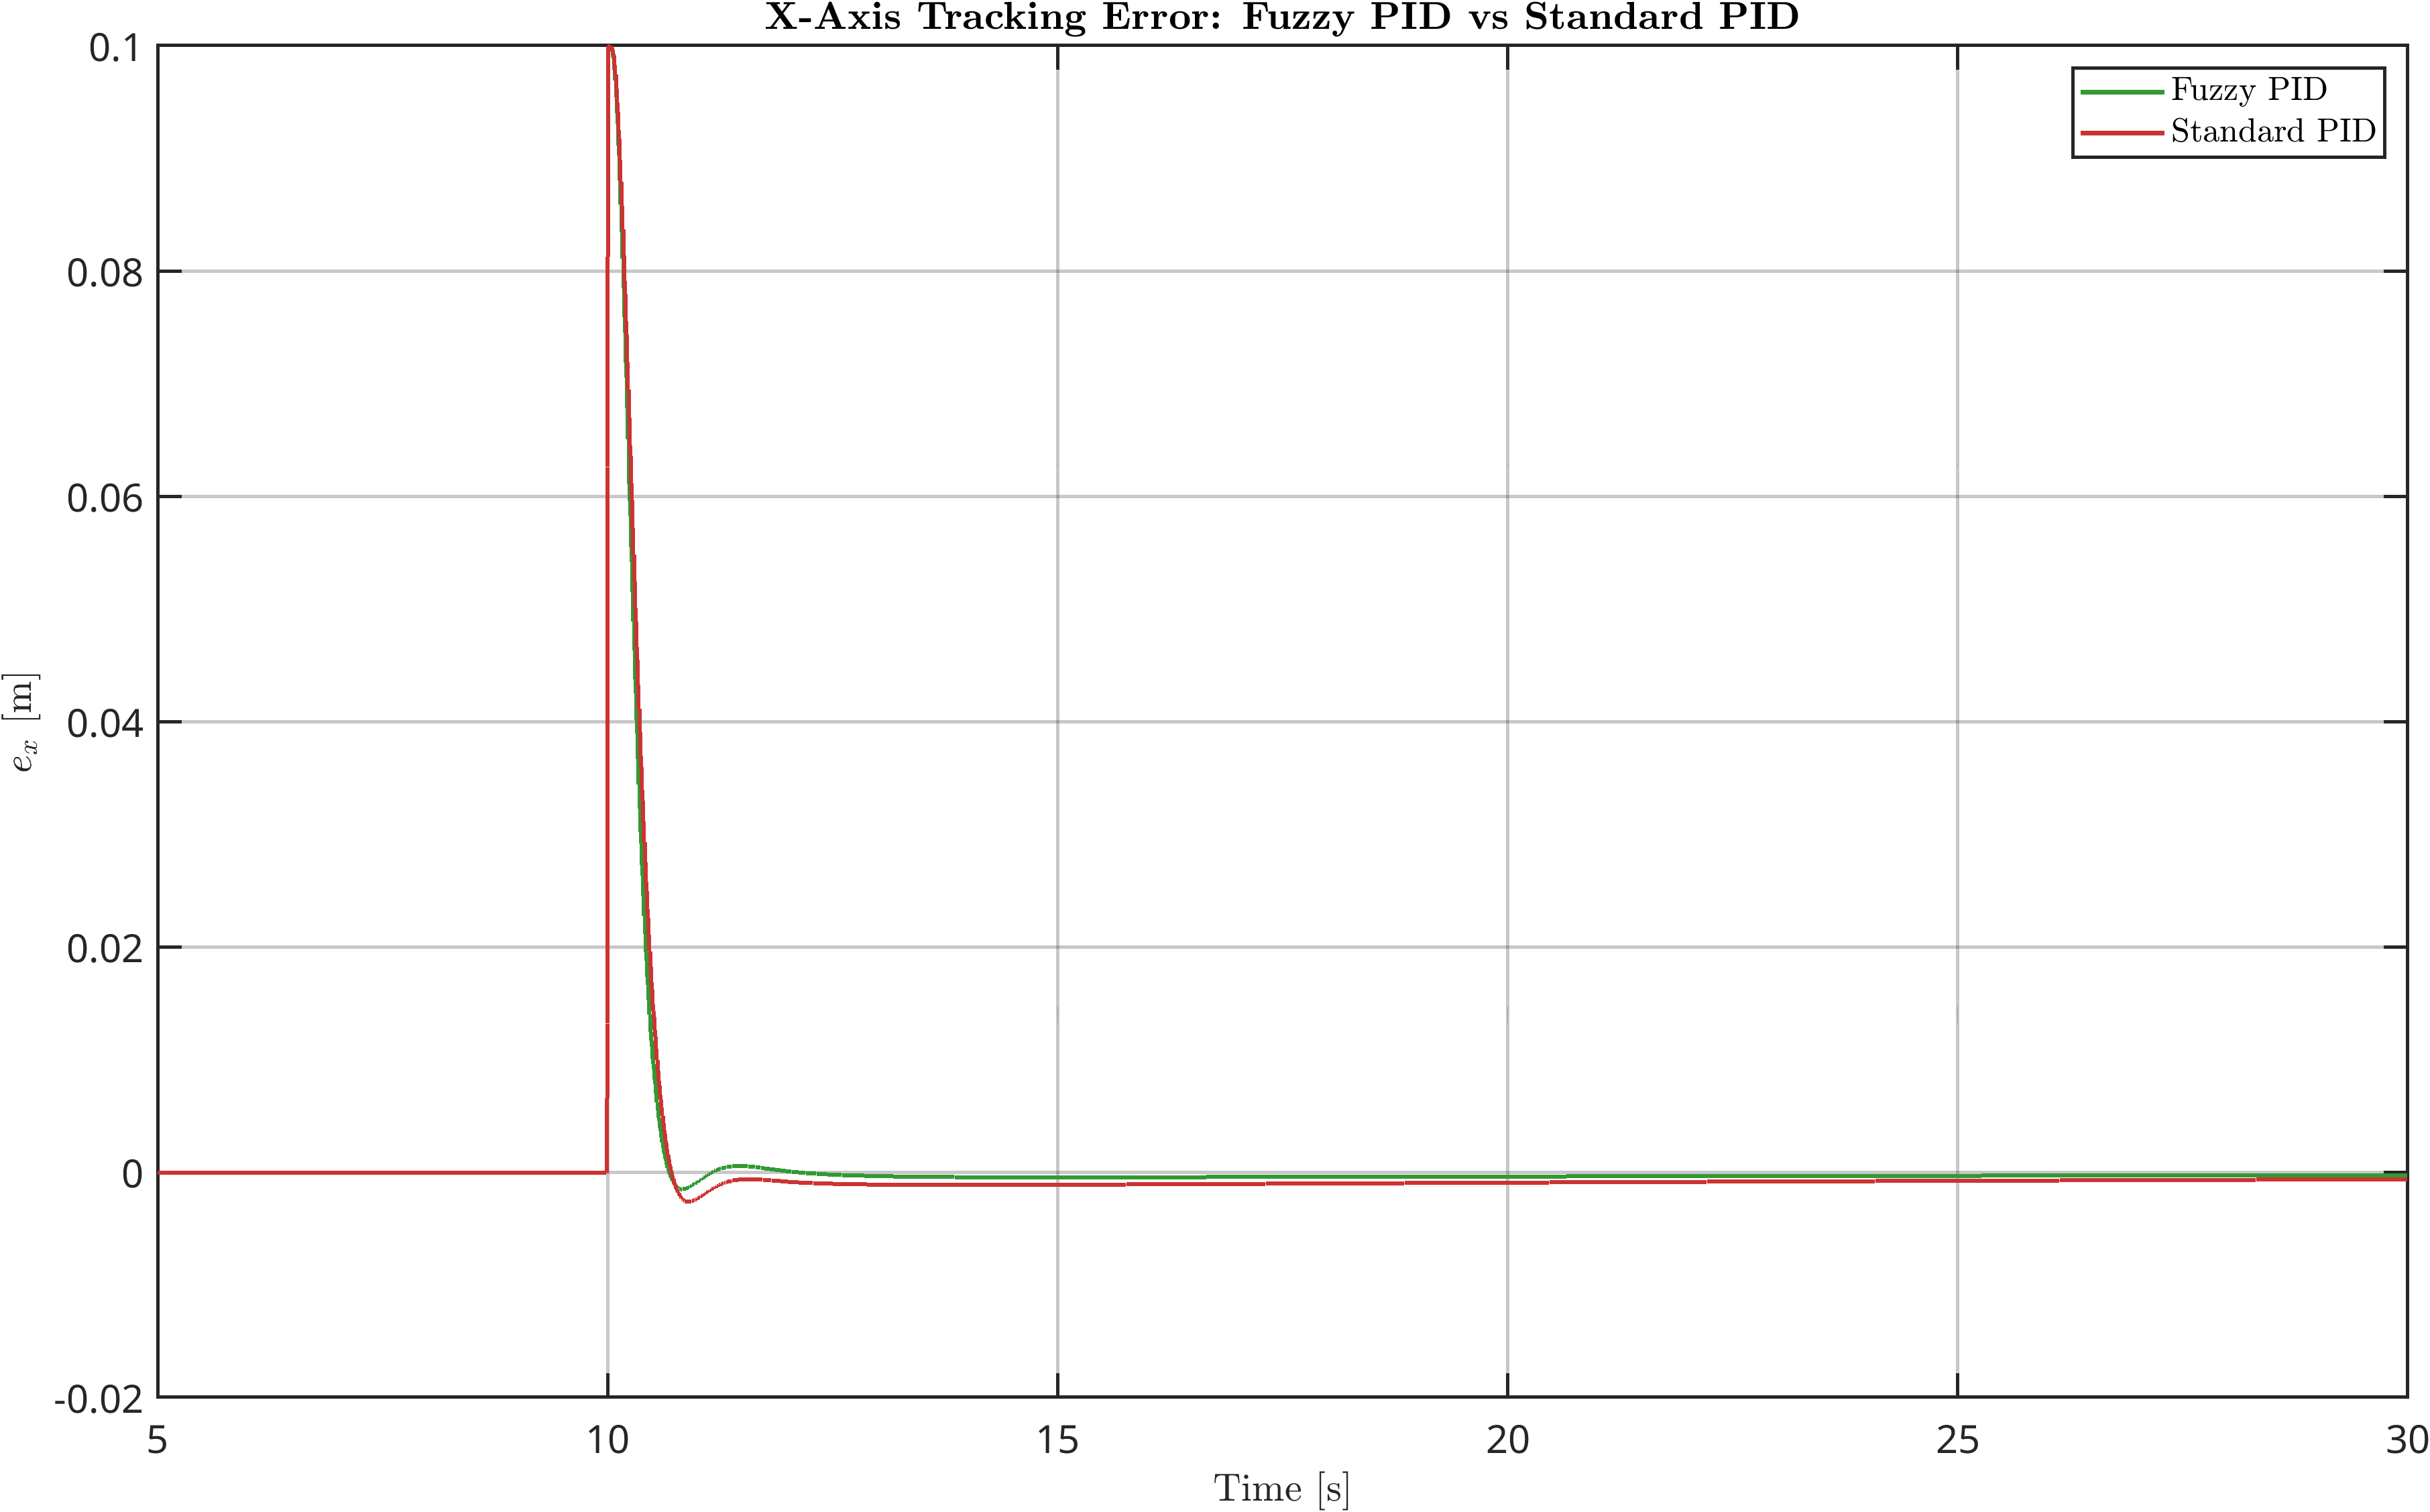
\includegraphics[width=0.48\textwidth]{img/step/x/error-comparison-x-step}}
	\\
	\subfloat[مقایسه تلاش کنترلی ($F_x$) دو کنترلر]{
		\label{fig:effort_comparison}
		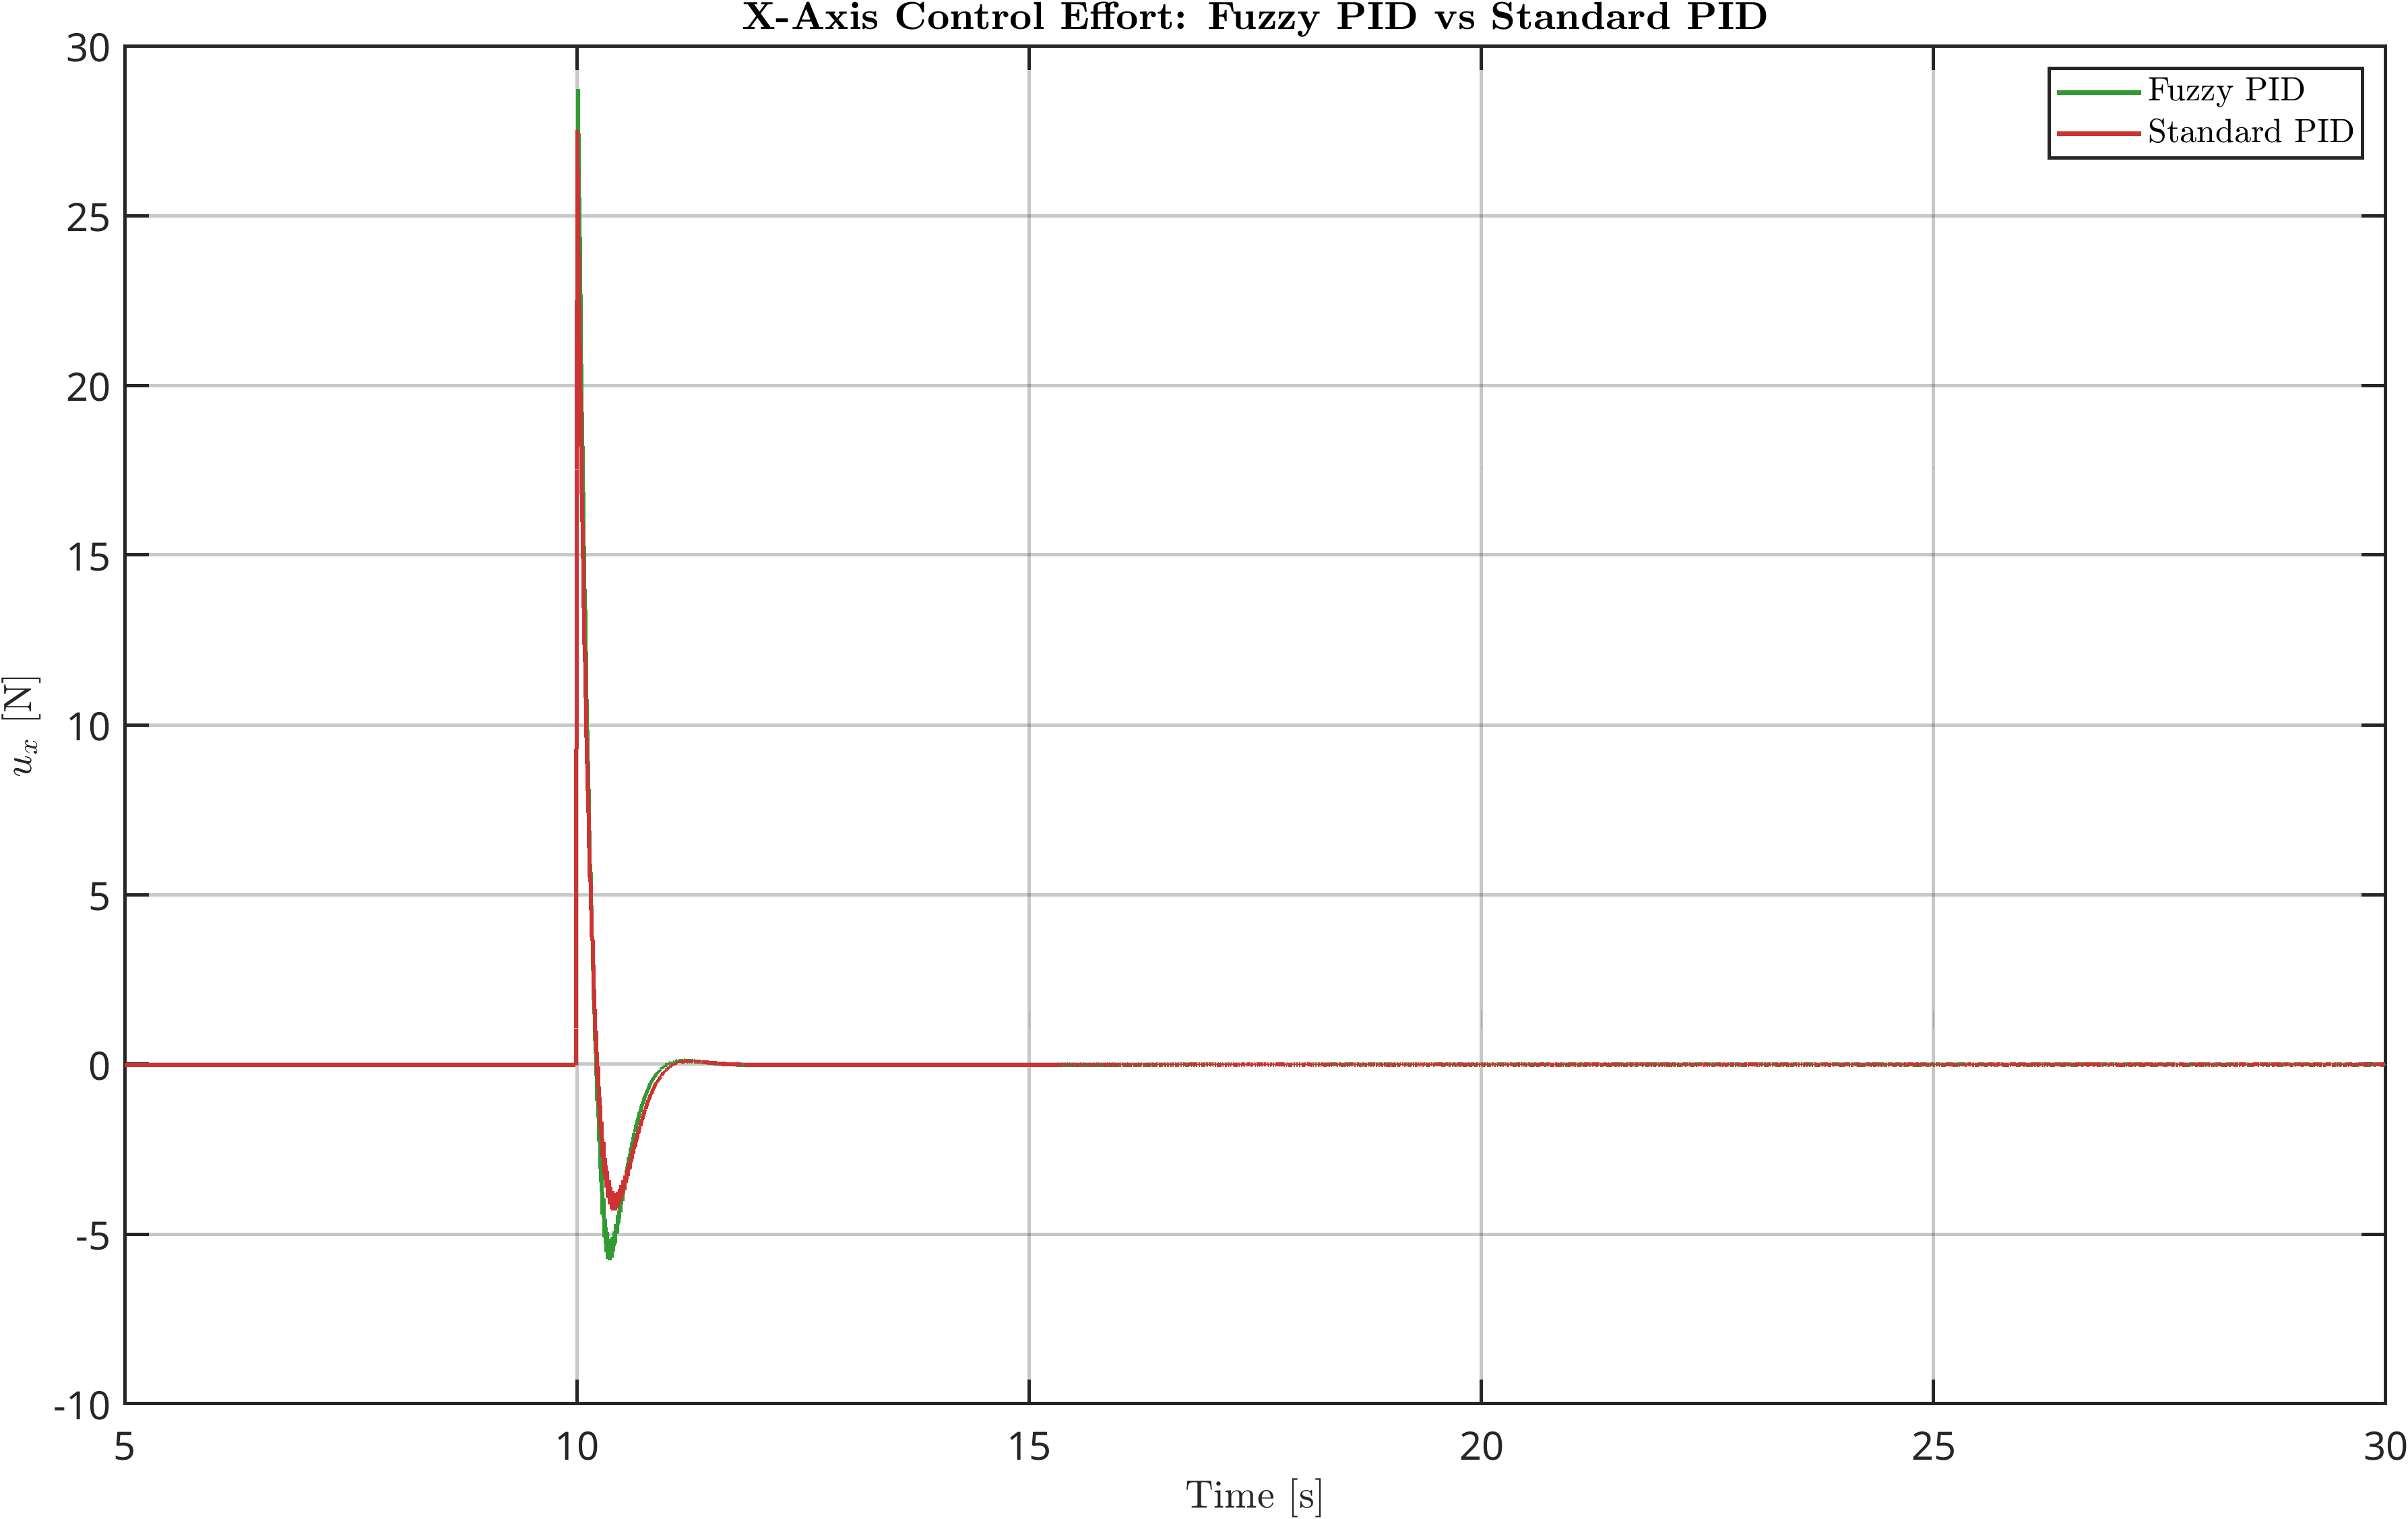
\includegraphics[width=0.75\textwidth]{img/step/x/control-effort-comparison-x-step}}
	\caption{مقایسه جامع عملکرد دو کنترلر فازی-PID و PID کلاسیک}
	\label{fig:comparison_all}
\end{figure}

\subsection{بحث و توجیه استفاده از کنترلر فازی}
\label{subsec:results-fuzzy-justification}

نتایج کمّی ارائه‌شده در بخش پیشین نشان داد که کنترلر فازی-PID در تمامی شاخص‌های عملکردی برتری محسوسی نسبت به PID کلاسیک دارد. با این حال، توجیه استفاده از این ساختار کنترلی صرفاً به بهبود اعداد در یک آزمون پله محدود نمی‌شود. دو مزیت بنیادین دیگر نیز وجود دارد که کنترلر فازی را به گزینه‌ای عملی و مناسب برای این کلاس از سیستم‌ها بدل می‌سازد.

نخست آنکه فرایند \textbf{تنظیم (\lr{Tuning})} یک کنترلر PID کلاسیک برای سیستم‌هایی نظیر MLPM که فاقد مدل ریاضی ساده و خطی هستند، به‌طور ذاتی دشوار و زمان‌بر است. در فضای شبیه‌سازی این پژوهش، به دلیل حضور موتور فیزیک \lr{DART}، دینامیک غیرخطی مغناطیسی، و نویز عددی، روش‌های مرسوم تنظیم مانند Ziegler-Nichols یا قطب‌گذاری عملاً قابل اعمال نبودند. در چنین شرایطی، چارچوب فازی با قواعد پیش‌تعریف‌شده (که بر اساس تجربه‌ی کنترلی و نه مدل دقیق ریاضی تدوین شده‌اند) به عنوان یک \textit{ابرتنظیم‌کننده} (\lr{Meta-Tuner}) عمل می‌کند. به این معنا که کافی است محدوده‌ی کلی بهره‌ها مشخص گردد و سپس سیستم فازی به صورت خودکار و لحظه‌ای، بهره‌های دقیق را متناسب با شرایط خطا و مشتق خطا تعیین نماید. در نتیجه، فرایند دشوار و چندبعدی تنظیم PID به یک تخمین ساده‌ی محدوده‌ی بهره‌ها تقلیل می‌یابد که این خود مزیتی قابل‌توجه در مراحل توسعه و پیاده‌سازی است.

دوم آنکه کنترلر فازی ذاتاً از \textbf{استواری (\lr{Robustness})} بیشتری در برابر عدم قطعیت‌های مدل برخوردار است. مدل استفاده‌شده در این پژوهش برای روابط نیرو و گشتاور، یک مدل تحلیلی اقتباس‌شده از مرجع \cite{RN10} می‌باشد. با این حال، در مسیر حرکت به سمت پیاده‌سازی فیزیکی، همواره اختلافاتی میان مدل و واقعیت (نظیر تلرانس‌های ساخت، اشباع مغناطیسی، نویز حسگرها و دینامیک‌های مدل‌نشده) بروز خواهد کرد. یک کنترلر PID با بهره‌های ثابت که برای یک مدل مشخص تنظیم شده باشد، در مواجهه با این عدم قطعیت‌ها ممکن است عملکرد مطلوب خود را از دست بدهد. در مقابل، کنترلر فازی بهره‌های خود را بر اساس خطای اندازه‌گیری‌شده (و نه صرفاً مدل پیش‌بینی‌شده) تنظیم می‌کند و از این رو، ظرفیت بیشتری برای سازگاری با دینامیک واقعی سیستم خواهد داشت. استفاده از این رویکرد در شبیه‌ساز، گامی اولیه و ضروری برای انتقال به سخت‌افزار فیزیکی است؛ چرا که همان استراتژی کنترلی، با حفظ قواعد فازی، قابلیت تطبیق با دینامیک واقعی سیستم را نیز خواهد داشت.

بنابراین، انتخاب کنترلر فازی-PID در این پژوهش نه تنها با بهبود شاخص‌های عملکرد کمّی تأیید می‌شود، بلکه به دلیل ساده‌سازی فرایند تنظیم و افزایش استواری در برابر عدم قطعیت‌ها، رویکردی مستدل و متناسب با اهداف بلندمدت این تحقیق محسوب می‌گردد.
%====================================================
\subsection{تلاش کنترلی و تخصیص جریان}
\label{subsec:results-control-effort}

نتایج ارائه‌شده در بخش‌های پیشین نشان داد که کنترل‌کننده‌ی فازی-PID طراحی‌شده قادر است وضعیت سیستم را در تمامی درجات آزادی با دقت مطلوب و در زمانی قابل قبول به مقادیر مرجع برساند. با این حال، صرف دستیابی به یک پاسخ پله‌ی رضایت‌بخش در محیط شبیه‌سازی، برای تضمین امکان‌پذیری پیاده‌سازی عملی کافی نیست. یک پلتفُرم مغناطیسی شناور، بر خلاف یک سیستم کنترل ایده‌آل، دارای عملگرهایی با محدودیت‌های فیزیکی ذاتی است. اگر فرامین کنترلی (نیروها و گشتاورهای مطلوب) بدون لحاظ این محدودیت‌ها به سیم‌پیچ‌ها ابلاغ شوند، ممکن است منجر به درخواست جریان‌های غیرقابل تأمین و در نتیجه عملکردی مغایر با آنچه شبیه‌ساز فیزیکی نشان می‌دهد، گردند. از این رو، در معماری کنترلی این پژوهش، حلقه‌ی تخصیص کنترلی به گونه‌ای طراحی شده است که پیش از اعمال پیچش\LTRfootnote{Wrench} نهایی به جسم متحرک در \lr{Gazebo}، قیود سخت‌افزاری سیم‌پیچ‌ها لحاظ گردد.

همان‌گونه که در بلوک‌دیاگرام کلی سیستم (فصل \ref{ch:method}) تشریح شد، مسیر سیگنال از کنترل‌کننده تا عملگر به صورت زیر است: نخست، پیچش مطلوب $W_{\text{des}}$ (خروجی کنترل‌کننده) به فضای جریان برده می‌شود. این نگاشت توسط وارون شبه‌مور-پنروز ماتریس $\Gamma$ و با بهره‌گیری از روش تجزیه مقادیر منفرد\LTRfootnote{SVD} انجام می‌پذیرد تا جریان‌های مرجع خام $I_{\text{raw}}$ برای ۱۶ سیم‌پیچ محاسبه شوند. در یک سیستم ایده‌آل، این جریان‌ها مستقیماً به سیم‌پیچ‌ها اعمال می‌گردند. اما در عمل، دو محدودیت اصلی بر روی این مقادیر اعمال می‌شود: بیشینه‌ی دامنه‌ی جریان و بیشینه‌ی نرخ تغییرات آن. پس از اعمال این قیود، جریان‌های اصلاح‌شده ($I_{\text{sat}}$) مجدداً از طریق ماتریس سینماتیک مستقیم $\Gamma$ به فضای پیچش بازگردانده می‌شوند و پیچش واقعی قابل تحقق ($W_{\text{act}}$) حاصل می‌آید که در نهایت به بدنه‌ی متحرک در شبیه‌ساز وارد می‌شود. تحلیل تلاش کنترلی و جریان‌های تخصیص‌یافته در این بخش، معطوف به همین زنجیره‌ی وارون و مستقیم، با در نظر گرفتن دو قید اساسی زیر است.

\textbf{۱. محدودیت دامنه‌ی جریان (اشباع).} بر اساس مشخصات فنی سیستم و مقالات مرجع، بیشینه‌ی جریان مجاز عبوری از هر سیم‌پیچ $I_{\max} = 9$ آمپر تعیین شده است. بنابراین، جریان‌های خام پس از خروج از بلوک سینماتیک وارون، از یک بلوک اشباع عبور می‌کنند تا هر مؤلفه‌ای که از این حد فراتر رود، در $\pm 9$ آمپر محدود گردد:
\begin{equation}
	I_{\text{sat,raw},j} = \text{sat}(I_{\text{raw},j},\, -9,\, 9),\quad j=1,\dots,16. 
	\label{eq:results-saturation}
\end{equation}

\textbf{۲. محدودیت نرخ تغییرات جریان (محدودکننده‌ی نرخ).} عملگرهای این سامانه، سیم‌پیچ‌های الکتریکی با خاصیت سلفی هستند. بنابر قانون القای الکترومغناطیسی، رابطه‌ی ولتاژ-جریان در یک سیم‌پیچ با اندوکتانس $L$ و مقاومت $R$ به صورت زیر است:
\begin{equation}
	V = L\frac{di}{dt} + R i.
	\label{eq:results-inductor}
\end{equation}
از این رابطه، نرخ تغییرات جریان به‌دست می‌آید:
\begin{equation}
	\frac{di}{dt} = \frac{V - R i}{L}.
	\label{eq:results-slew-rate}
\end{equation}

از آن‌جا که نرخ تغییرات جریان تابعی از ولتاژ اعمالی، مقاومت و اندوکتانس سیم‌پیچ است، در بدترین حالت عملکردی (نزدیک به جریان نامی) مقدار این نرخ محدود می‌گردد. به منظور رعایت یک حاشیه‌ی اطمینان محافظه‌کارانه و اطمینان از امکان‌پذیری تأمین جریان در سخت‌افزار واقعی، یک محدودیت نرخ ثابت و متقارن برابر با $80$ آمپر بر ثانیه برای تمامی سیم‌پیچ‌ها به‌عنوان قید طراحی در شبیه‌سازی‌ها اعمال گردیده است. بلوک \lr{rate limiter} تعبیه‌شده در مسیر تخصیص، چنانچه شیب سیگنال جریان مرجع از این مقدار فراتر رود، آن را به $80$ آمپر بر ثانیه محدود می‌کند:
\begin{equation}
	\left|\frac{d I_{\text{cmd},j}}{dt}\right| \le 80\;\text{A/s},\quad j=1,\dots,16.
	\label{eq:results-rate-limit}
\end{equation}
بدین ترتیب، تمامی نتایج ارائه‌شده در این فصل با لحاظ این محدودیت نرخ به‌دست آمده‌اند و حتی در شدیدترین مانورهای کنترلی نیز جریان‌های درخواستی همواره در محدوده‌ای که سخت‌افزار قادر به تأمین آن است، باقی می‌مانند.

با اعمال این دو قید بر روی جریان‌های تخصیص‌یافته، \textbf{پیچش عملی} $W_{\text{act}}$ که در نهایت به شبیه‌ساز فیزیکی تزریق می‌شود، نه فقط یک سیگنال کنترلی ریاضی، بلکه بازتابی وفادار از توانمندی عملگرهای الکترومغناطیسی خواهد بود. در ادامه، ابتدا پیچش‌های خروجی و سپس جریان‌های سیم‌پیچ‌ها برای هر یک از درجات آزادی خطی و زاویه‌ای، با در نظر گرفتن هر دو محدودیت فوق، تحلیل و ارائه می‌گردند.

%----------------------------------------------------
\subsubsection{تحلیل پیچش خروجی در درجات آزادی خطی}
\label{subsubsec:results-wrench-linear}

پیچش‌های عملی ($W_{\text{act}}$) که پس از عبور از زنجیره‌ی وارون و مستقیم سینماتیک و اعمال قیود سخت‌افزاری به بدنه‌ی متحرک در \lr{Gazebo} وارد شده‌اند، برای پاسخ‌های پله‌ی محورهای $X$، $Y$ و $Z$ در شکل‌های \ref{fig:results-wrench-xy} و \ref{fig:results-wrench-z} ارائه شده‌اند. تحلیل این سیگنال‌ها نشان می‌دهد که رفتار کنترلی مشاهده‌شده با منطق تطبیقی کنترل‌کننده‌ی فازی که پیش‌تر تشریح شد، هم‌خوانی کامل دارد و قیود فیزیکی به‌طور مؤثری فرم نهایی موج را شکل داده‌اند.

در حرکت گام محور $X$، اوج نیروی $F_x$ به تقریباً $30$ نیوتن می‌رسد. این جهش مثبت و قابل‌توجه، تأمین‌کننده‌ی شتاب اولیه‌ی لازم برای غلبه بر اینرسی جسم $6.6$ کیلوگرمی و دستیابی به زمان خیز گزارش‌شده در جدول \ref{tab:results-linear-metrics} است. بلافاصله پس از این اوج، نیرو به ناحیه‌ی منفی (حدود $-5$ نیوتن) فرو می‌افتد. این فروافتادگی جبرانی، دقیقاً مطابق با مکانیزم «فروافتادگی ـ جهش» سیستم فازی است که در بخش \ref{subsubsec:results-fuzzy-x} تحلیل شد: هنگام دور شدن خطا از صفر، بهره‌ی تناسبی به‌طور موقت کاهش می‌یابد تا از فراجهش جلوگیری کند، و متعاقباً یک پالس ترمزی منفی برای بازگرداندن سریع خطا به سمت صفر اعمال می‌شود. پس از این گذرای کوتاه، نیرو با نوسانات میرا شونده‌ای حول صفر تثبیت می‌گردد، که با میرایی متناظر در نمودار ضرایب کنترل‌کننده (شکل \ref{fig:results-fuzzy-x-gains}) هم‌زمان است. رفتار محور $Y$، به دلیل تقارن ساختاری، تصویری مشابه با دامنه‌های یکسان ارائه می‌دهد.

نکته‌ی قابل تأمل در هر دو حرکت صفحه‌ای $X$ و $Y$، پیدایش نیروها و گشتاورهای ناخواسته در سایر درجات آزادی است. در مقیاس دامنه‌های بزرگ $F_x$ یا $F_y$، این مؤلفه‌های پارازیتی کوچک به نظر می‌رسند، اما وجود آن‌ها بیان‌گر یک مشخصه‌ی ذاتی سیستم است: از آنجا که عملگرها (سیم‌پیچ‌ها) میان تمامی درجات آزادی مشترک هستند و ماتریس $\Gamma$ کوپلینگ عرضی را ناگزیر می‌سازد، یک فرمان خالص در یک راستا، به‌طور ذاتی توزیعی از جریان‌ها را می‌طلبد که مؤلفه‌های کوچکی در راستاهای دیگر نیز تولید می‌کنند. با این حال، این اغتشاشات درونی، به سرعت توسط کنترل‌کننده‌های مستقل همان محورها تشخیص داده شده و با دامنه‌ای محدود می‌را می‌شوند.

تحلیل پیچش محور $Z$ تصویری از یک فاز کنترلی کاملاً متفاوت ارائه می‌دهد. پیش از آغاز پله‌ی ارتفاع، و در حالی که جسم هنوز در وضعیت روی زمین (\lr{OnGround}) یا در آستانه‌ی برخاستن قرار دارد، نیروی $F_z$ از صفر به تدریج به حدود $66$ نیوتن افزایش می‌یابد. این رشد تدریجی، به‌مدد مقداردهی اولیه‌ی ایمن و فیلتر \lr{NaN} تعبیه‌شده، از جهش ناگهانی در لحظه‌ی اتصال حلقه جلوگیری می‌کند. با رسیدن به این سطح پایه که اندکی کمتر از وزن کامل ($mg \approx 68$ N) است، سیستم در آستانه‌ی خنثی‌سازی گرانش قرار می‌گیرد. سپس، هم‌زمان با فعال‌سازی پله‌ی ارتفاع توسط ماشین حالت (ورود به فاز \lr{Levitating})، یک جهش قائم نیرو تا حدود $160$ نیوتن رخ می‌دهد. این پیک، که بیش از دو برابر نیروی وزن است، انرژی لازم برای شتاب‌دهی عمودی اولیه را فراهم می‌آورد. پس از آن، نیرو با نوساناتی میرا به همان مقدار پایه‌ی $66$ نیوتن بازمی‌گردد و سیستم را در ارتفاع جدید معلق نگاه می‌دارد. شایان ذکر است که در طول این گذار، سایر درجات آزادی ($F_x, F_y$ و گشتاورها) به دلیل عملکرد ماشین حالت دو فازی و غیرفعال بودن حلقه‌های کنترلی آن‌ها در فاز روی زمین، دقیقاً روی صفر باقی می‌مانند و تنها پس از پایداری ارتفاع وارد مدار می‌شوند. این جداسازی تمیز فازها، از بروز تقابل ناخواسته میان کنترل‌کننده‌ها در لحظه‌ی برخاستن جلوگیری کرده است.


\begin{figure}[htbp]
	\centering
	\subfloat[$X$]{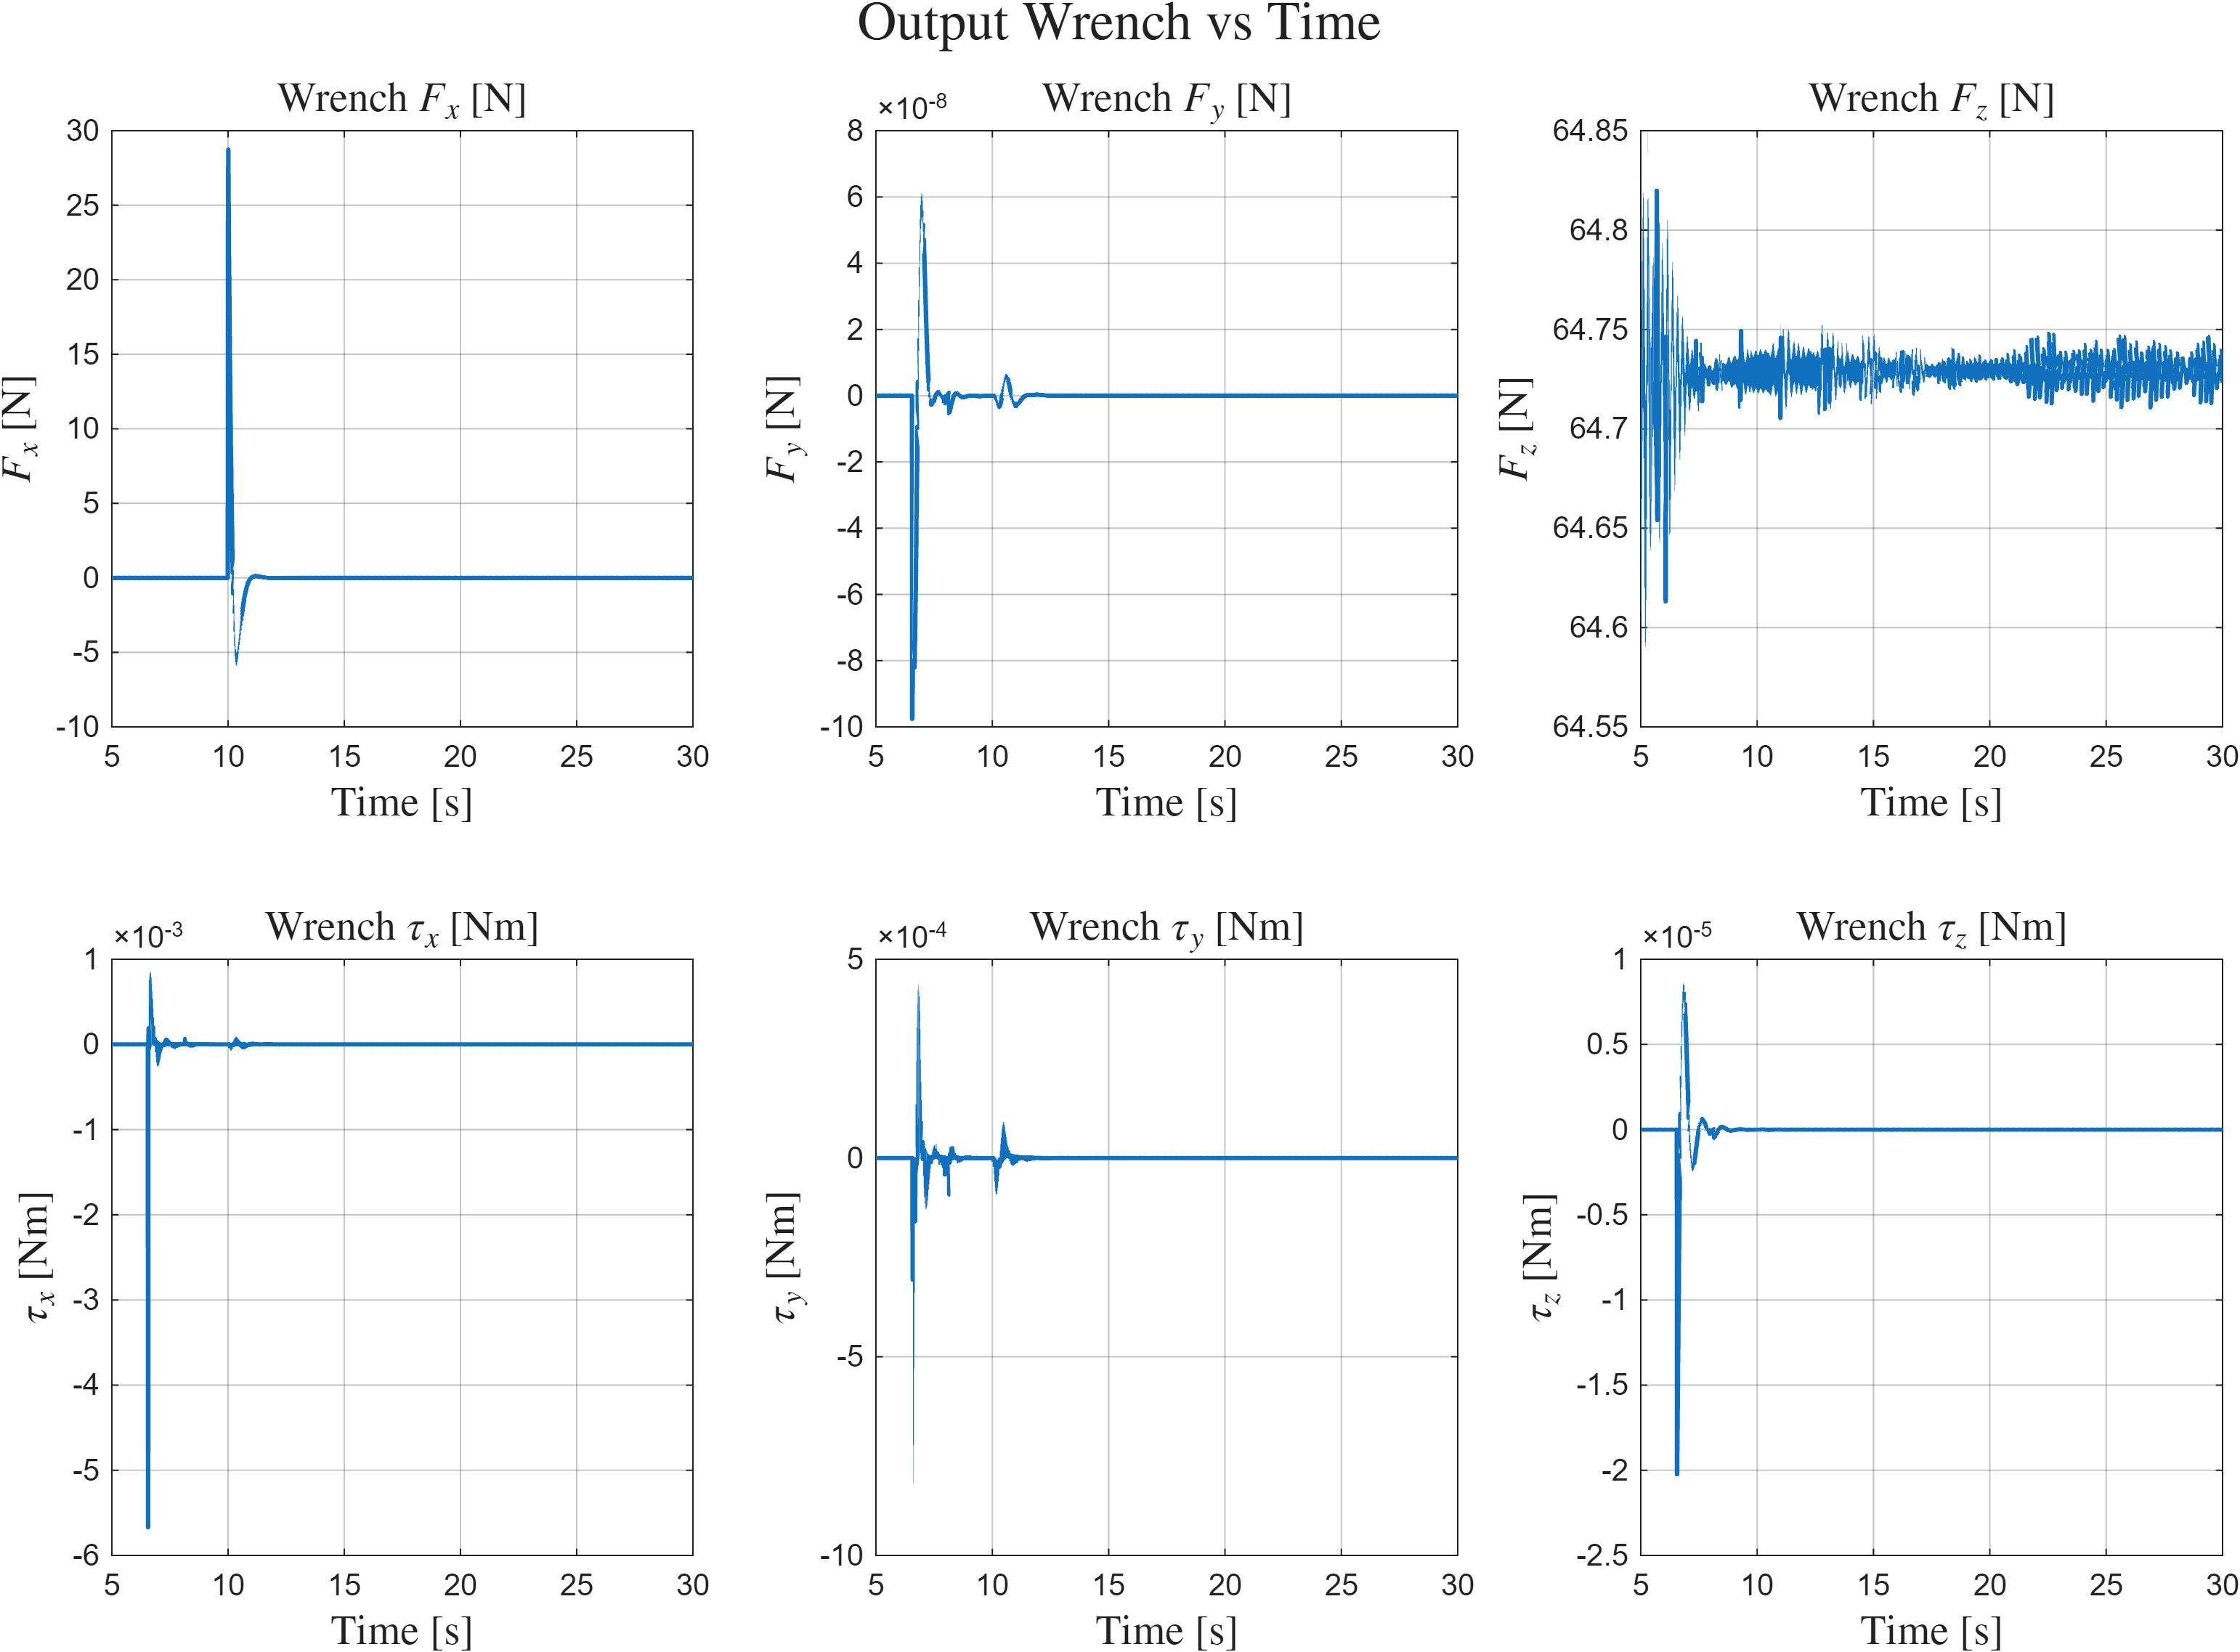
\includegraphics[width=0.48\textwidth]{img/step/x/output_wrench}}
	\hfill
	\subfloat[$Y$]{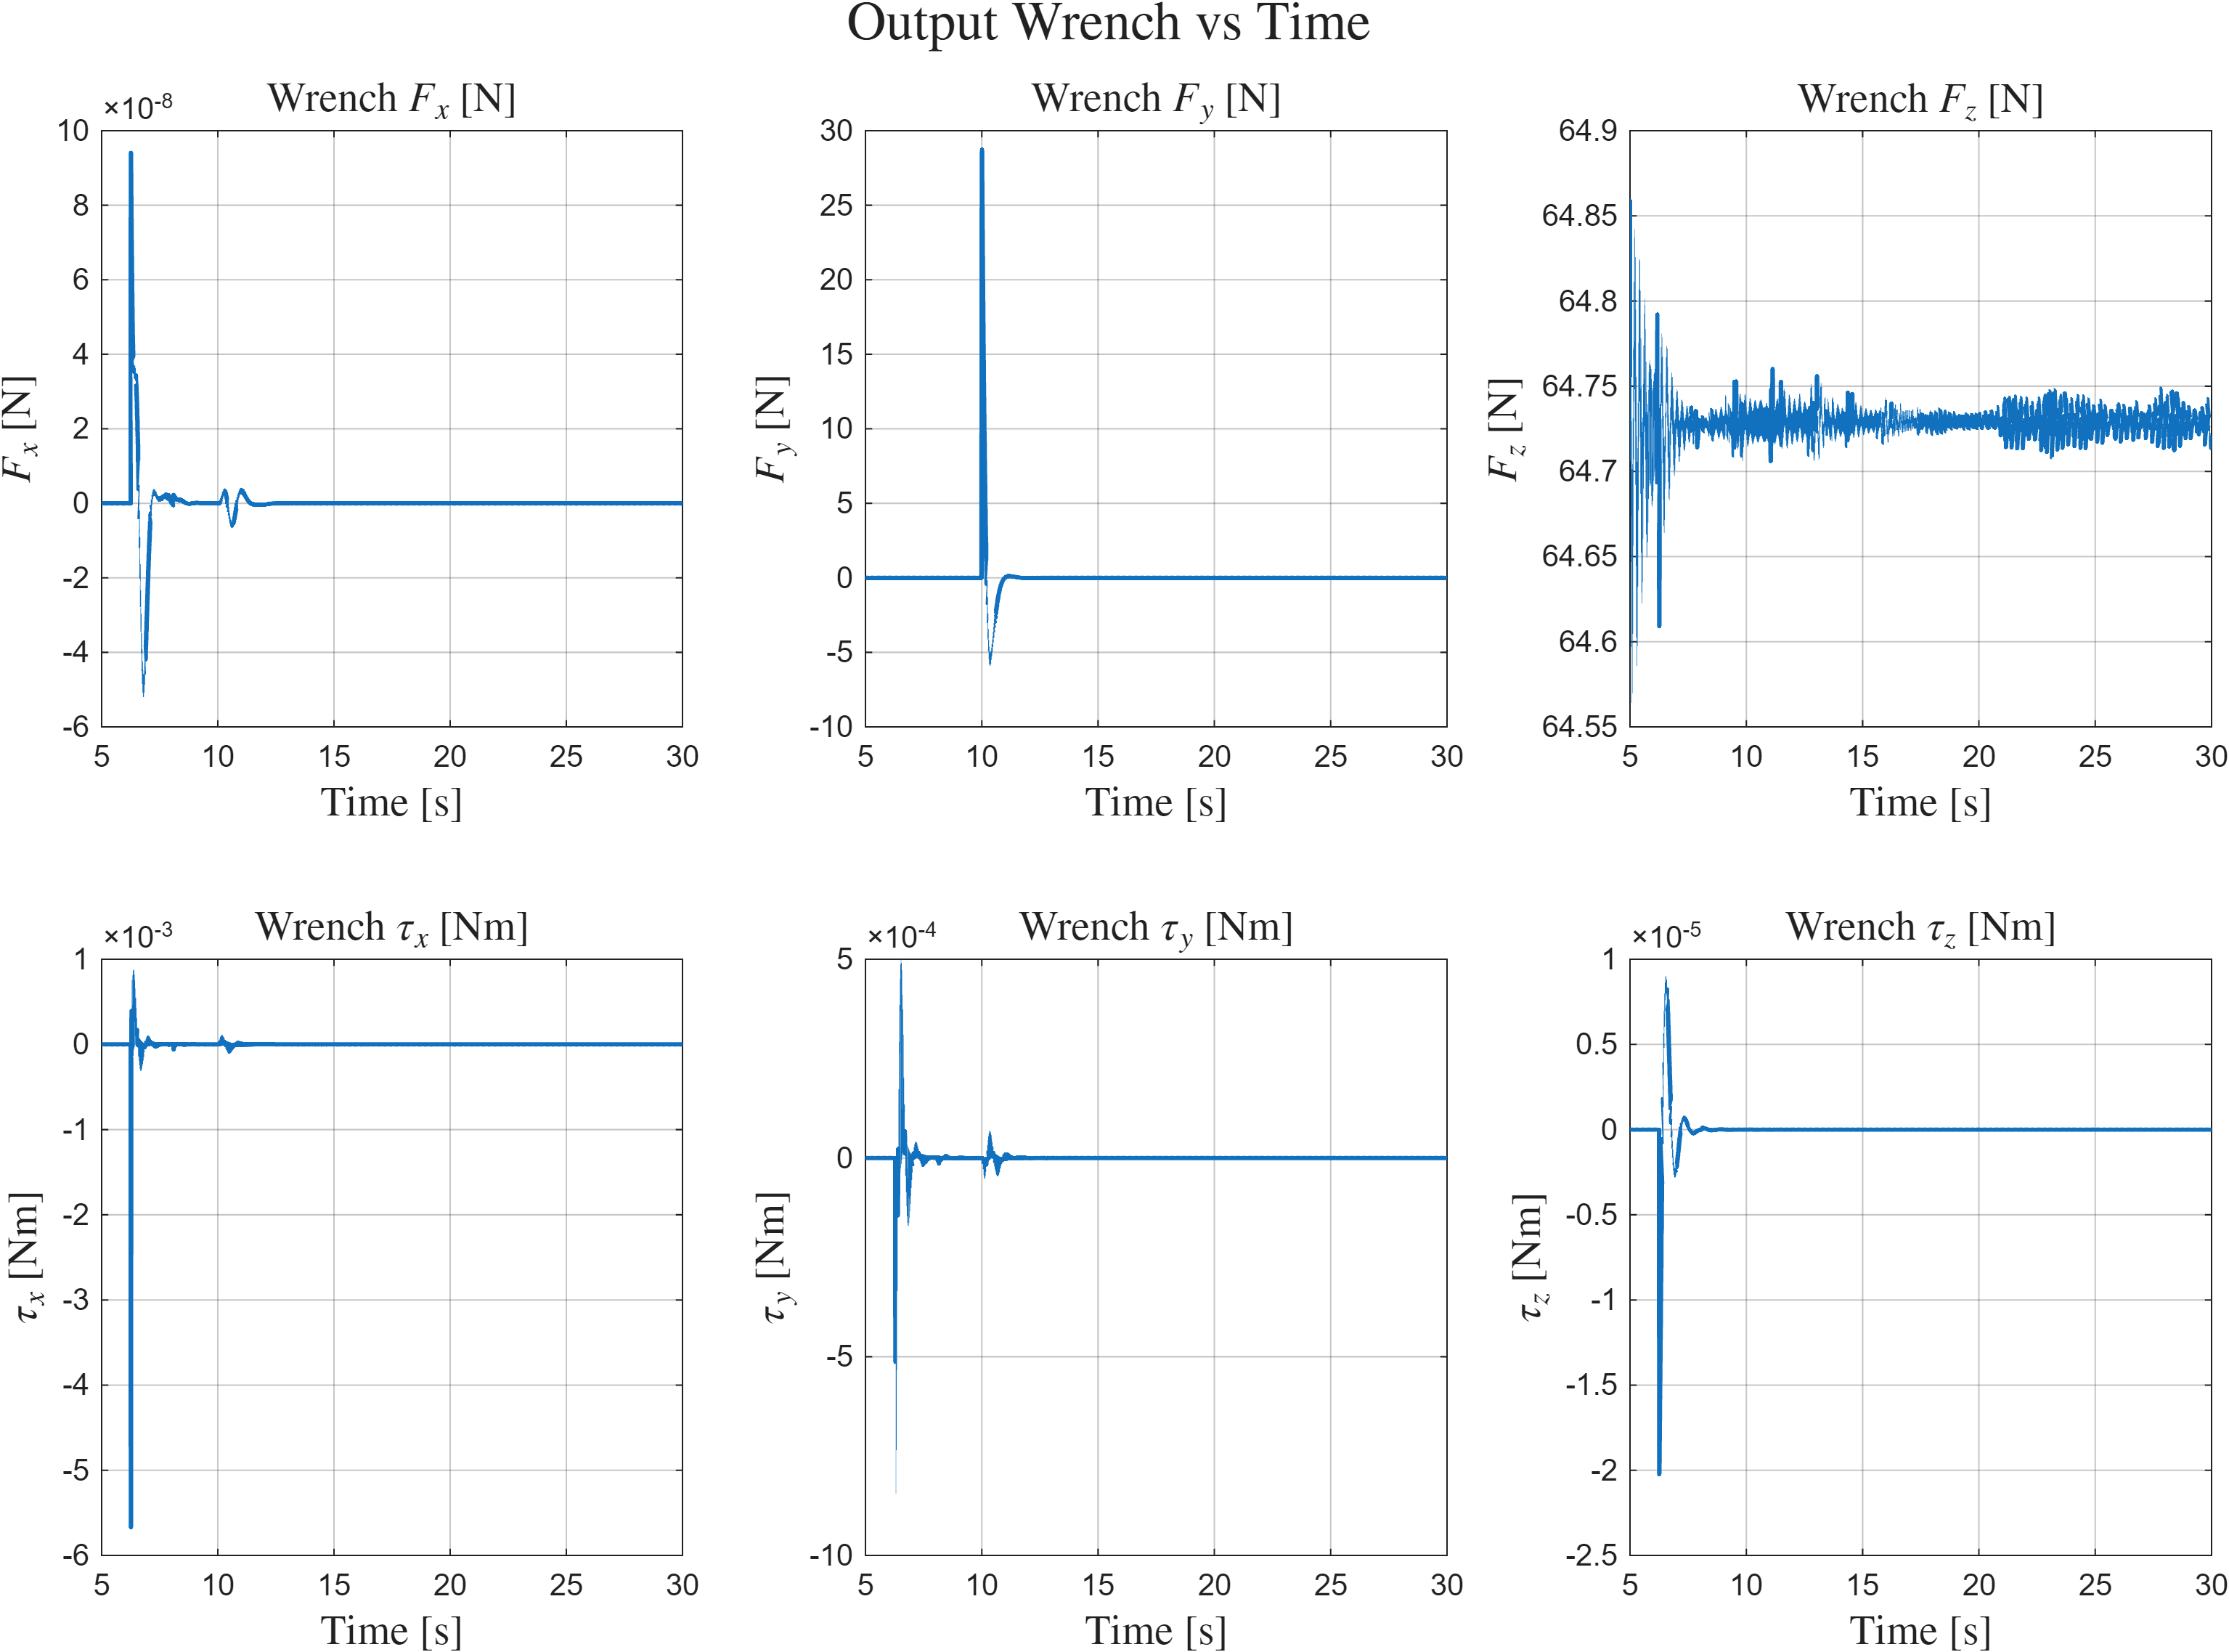
\includegraphics[width=0.48\textwidth]{img/step/y/output_wrench}}
	
	\caption{پیچش خروجی در درجات آزادی خطی $X$ و $Y$}
	\label{fig:results-wrench-xy}
\end{figure}

\begin{figure}[htbp]
	\centering
	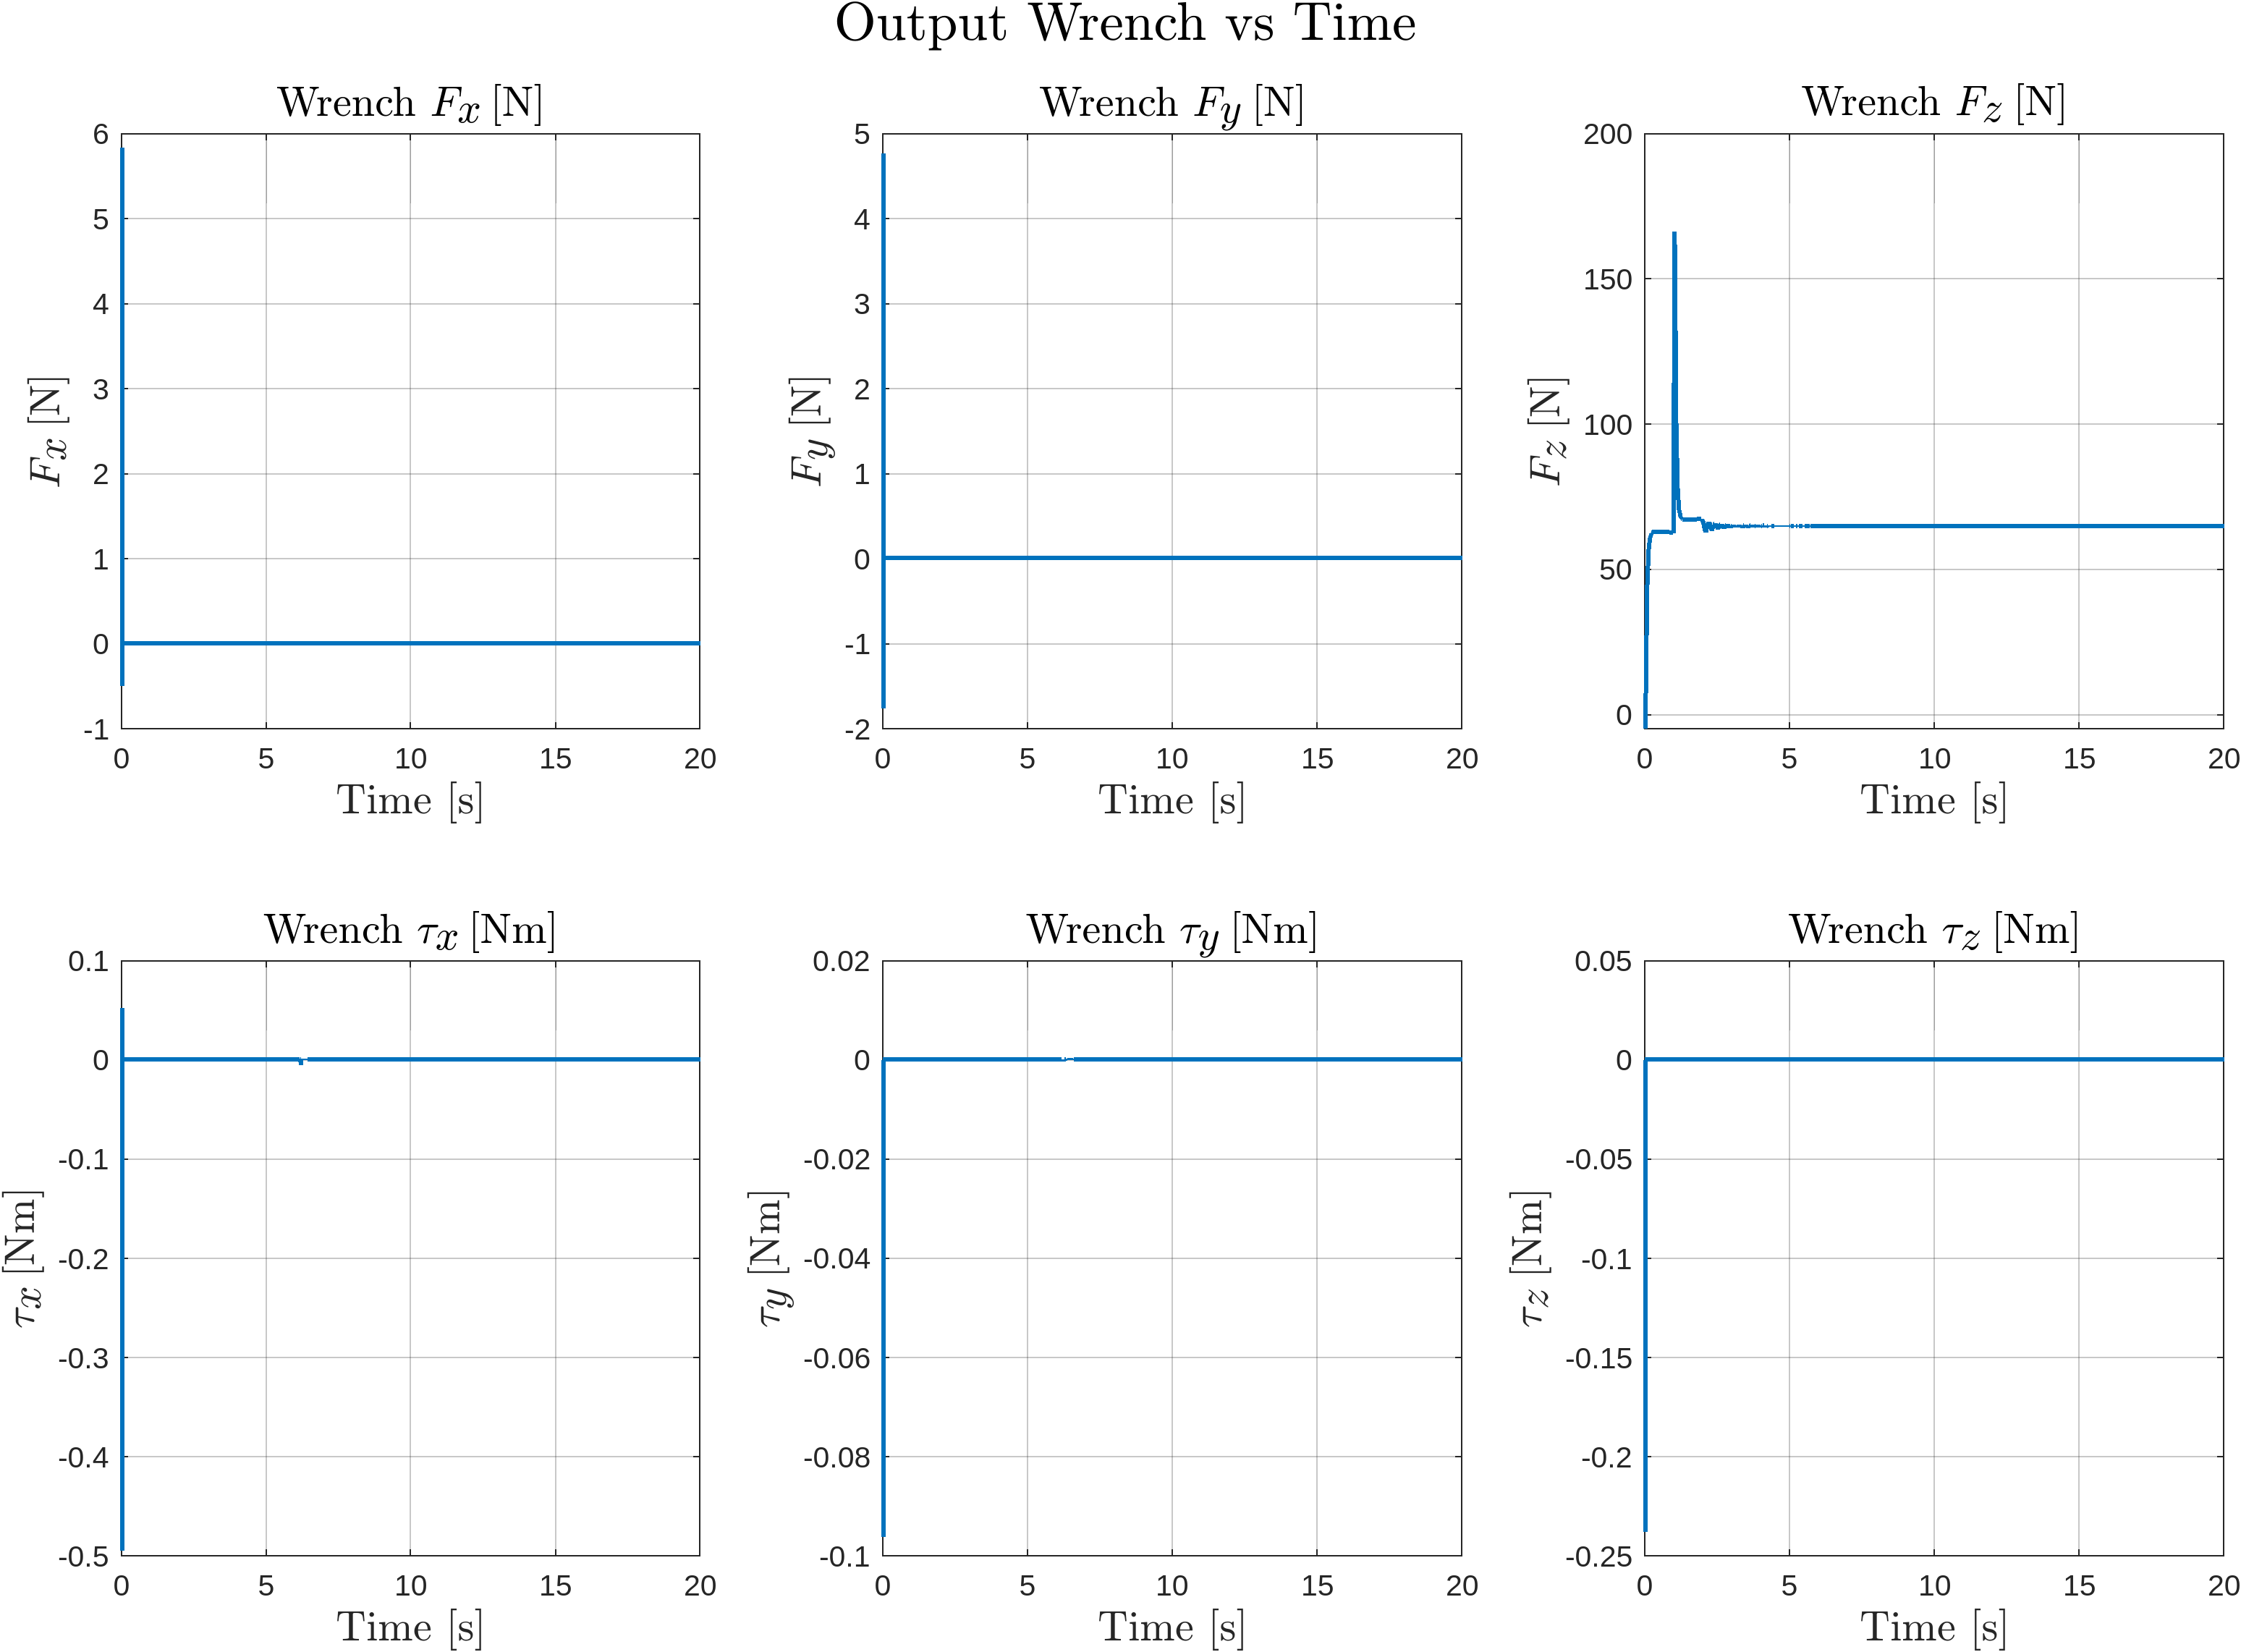
\includegraphics[width=0.75\textwidth]{img/step/z/output_wrench}
	\caption{پیچش خروجی در درجه آزادی $Z$}
	\label{fig:results-wrench-z}
\end{figure}

%----------------------------------------------------
\subsubsection{تحلیل پیچش خروجی در درجات آزادی زاویه‌ای}
\label{subsubsec:results-wrench-angular}

شکل‌های \ref{fig:results-wrench-alpha-beta} و \ref{fig:results-wrench-gamma} که پیچش خروجی را برای محورهای $\alpha$، $\beta$ و $\gamma$ نمایش می‌دهند، گواه آن هستند که کنترل‌کننده‌ی فازی-PID در فضای زاویه‌ای نیز الگوی تطبیقی مشابهی را با موفقیت به اجرا گذاشته است. با اعمال پله‌ی زاویه‌ای به $\alpha$ یا $\beta$، گشتاور حول محور مربوطه یک جهش تیز از صفر به حدود $4.2$ نیوتن‌متر را تجربه می‌کند. این پیک مثبت، نقش شتاب‌دهنده‌ی اولیه برای غلبه بر اینرسی دورانی کوچک ($I_{xx}=I_{yy}=0.06$ kg·m²) و دستیابی به زمان خیز سریع (حدود $0.3$ ثانیه) را ایفا می‌کند. بلافاصله پس از این اوج، گشتاور به سرعت کاهش یافته و به مقادیر منفی جزئی، اما ماندگارتر، فرو می‌افتد. این فروافتادگی جبرانی، که در تطابق کامل با منطق «جهش جبرانی» سیستم فازی (تحلیل‌شده در بخش \ref{subsubsec:results-fuzzy-x}) است، به‌منزله‌ی یک پالس ترمزی برای جلوگیری از فراجهش و استقرار سریع زاویه عمل می‌کند. سپس گشتاور با نوسانات میرا شونده به سمت صفر بازمی‌گردد و در حالت ماندگار هیچ تلاش کنترلی دائمی برای حفظ زاویه‌ی کوچک مطلوب نیاز نیست.

هم‌زمان با این جهش اصلی، یک اغتشاش متقاطع در محور متعامد القا می‌شود. برای مثال، پله‌ی $\alpha$ نوسانی با دامنه‌ی حداکثر $0.1$ نیوتن‌متر در $\beta$ پدید می‌آورد و بالعکس. این کوپلینگ ناخواسته، پیامد مستقیم اشتراک عملگرها (سیم‌پیچ‌ها) در تولید گشتاور حول هر دو محور است؛ توزیع جریان لازم برای ایجاد $T_x$، به‌ناچار مؤلفه‌ی اندکی $T_y$ نیز تولید می‌کند. نکته‌ی حائز اهمیت آن است که کنترل‌کننده‌ی مستقل محور متأثر، بلافاصله این اغتشاش را تشخیص داده و با اعمال گشتاور متقابل، آن را در همین دامنه‌ی کوچک مستهلک می‌سازد، به‌گونه‌ای که تأثیر آن بر دقت ردیابی زاویه‌ای (جدول \ref{tab:results-angular-metrics}) ناچیز باقی می‌ماند. سایر درجات آزادی (نیروهای خطی و $\gamma$) در این بین، واکنش قابل‌توجهی نشان نمی‌دهند.

پاسخ گشتاوری محور $\gamma$ الگویی مشابه اما با دامنه‌ای تقریباً نصف ارائه می‌دهد: جهش اولیه حدود $2$ نیوتن‌متر است که با گذر از یک فاز منفی خفیف، به سرعت به صفر می‌را می‌شود. این تفاوت کمّی با مقادیر $4.2$ نیوتن‌متری $\alpha$ و $\beta$، بازتابی از ممان اینرسی بزرگ‌تر حول محور $z$ ($I_{zz}=0.12$ kg·m²) و نیز تفاوت در اندرکنش مغناطیسی ذاتی این درجه آزادی است. با وجود دامنه‌ی کمتر، رفتار کیفی (جهش، فروافتادگی، میرایی) همچنان برقرار است و نشان می‌دهد که ساختار فازی، با موفقیت خود را با دینامیک متفاوت هر محور وفق داده و پاسخی متناسب با ظرفیت عملگری آن فراهم آورده است. در تمامی موارد، منحنی‌های گشتاور فاقد شوک‌های فرکانس بالا و ناپیوستگی هستند که این امر، مرهون عملکرد محدودکننده‌ی نرخ جریان و فیلتر مشتق در حفظ نرمی فرامین اعمالی به شبیه‌ساز است.

\begin{figure}[htbp]
	\centering
	\subfloat[$\alpha$]{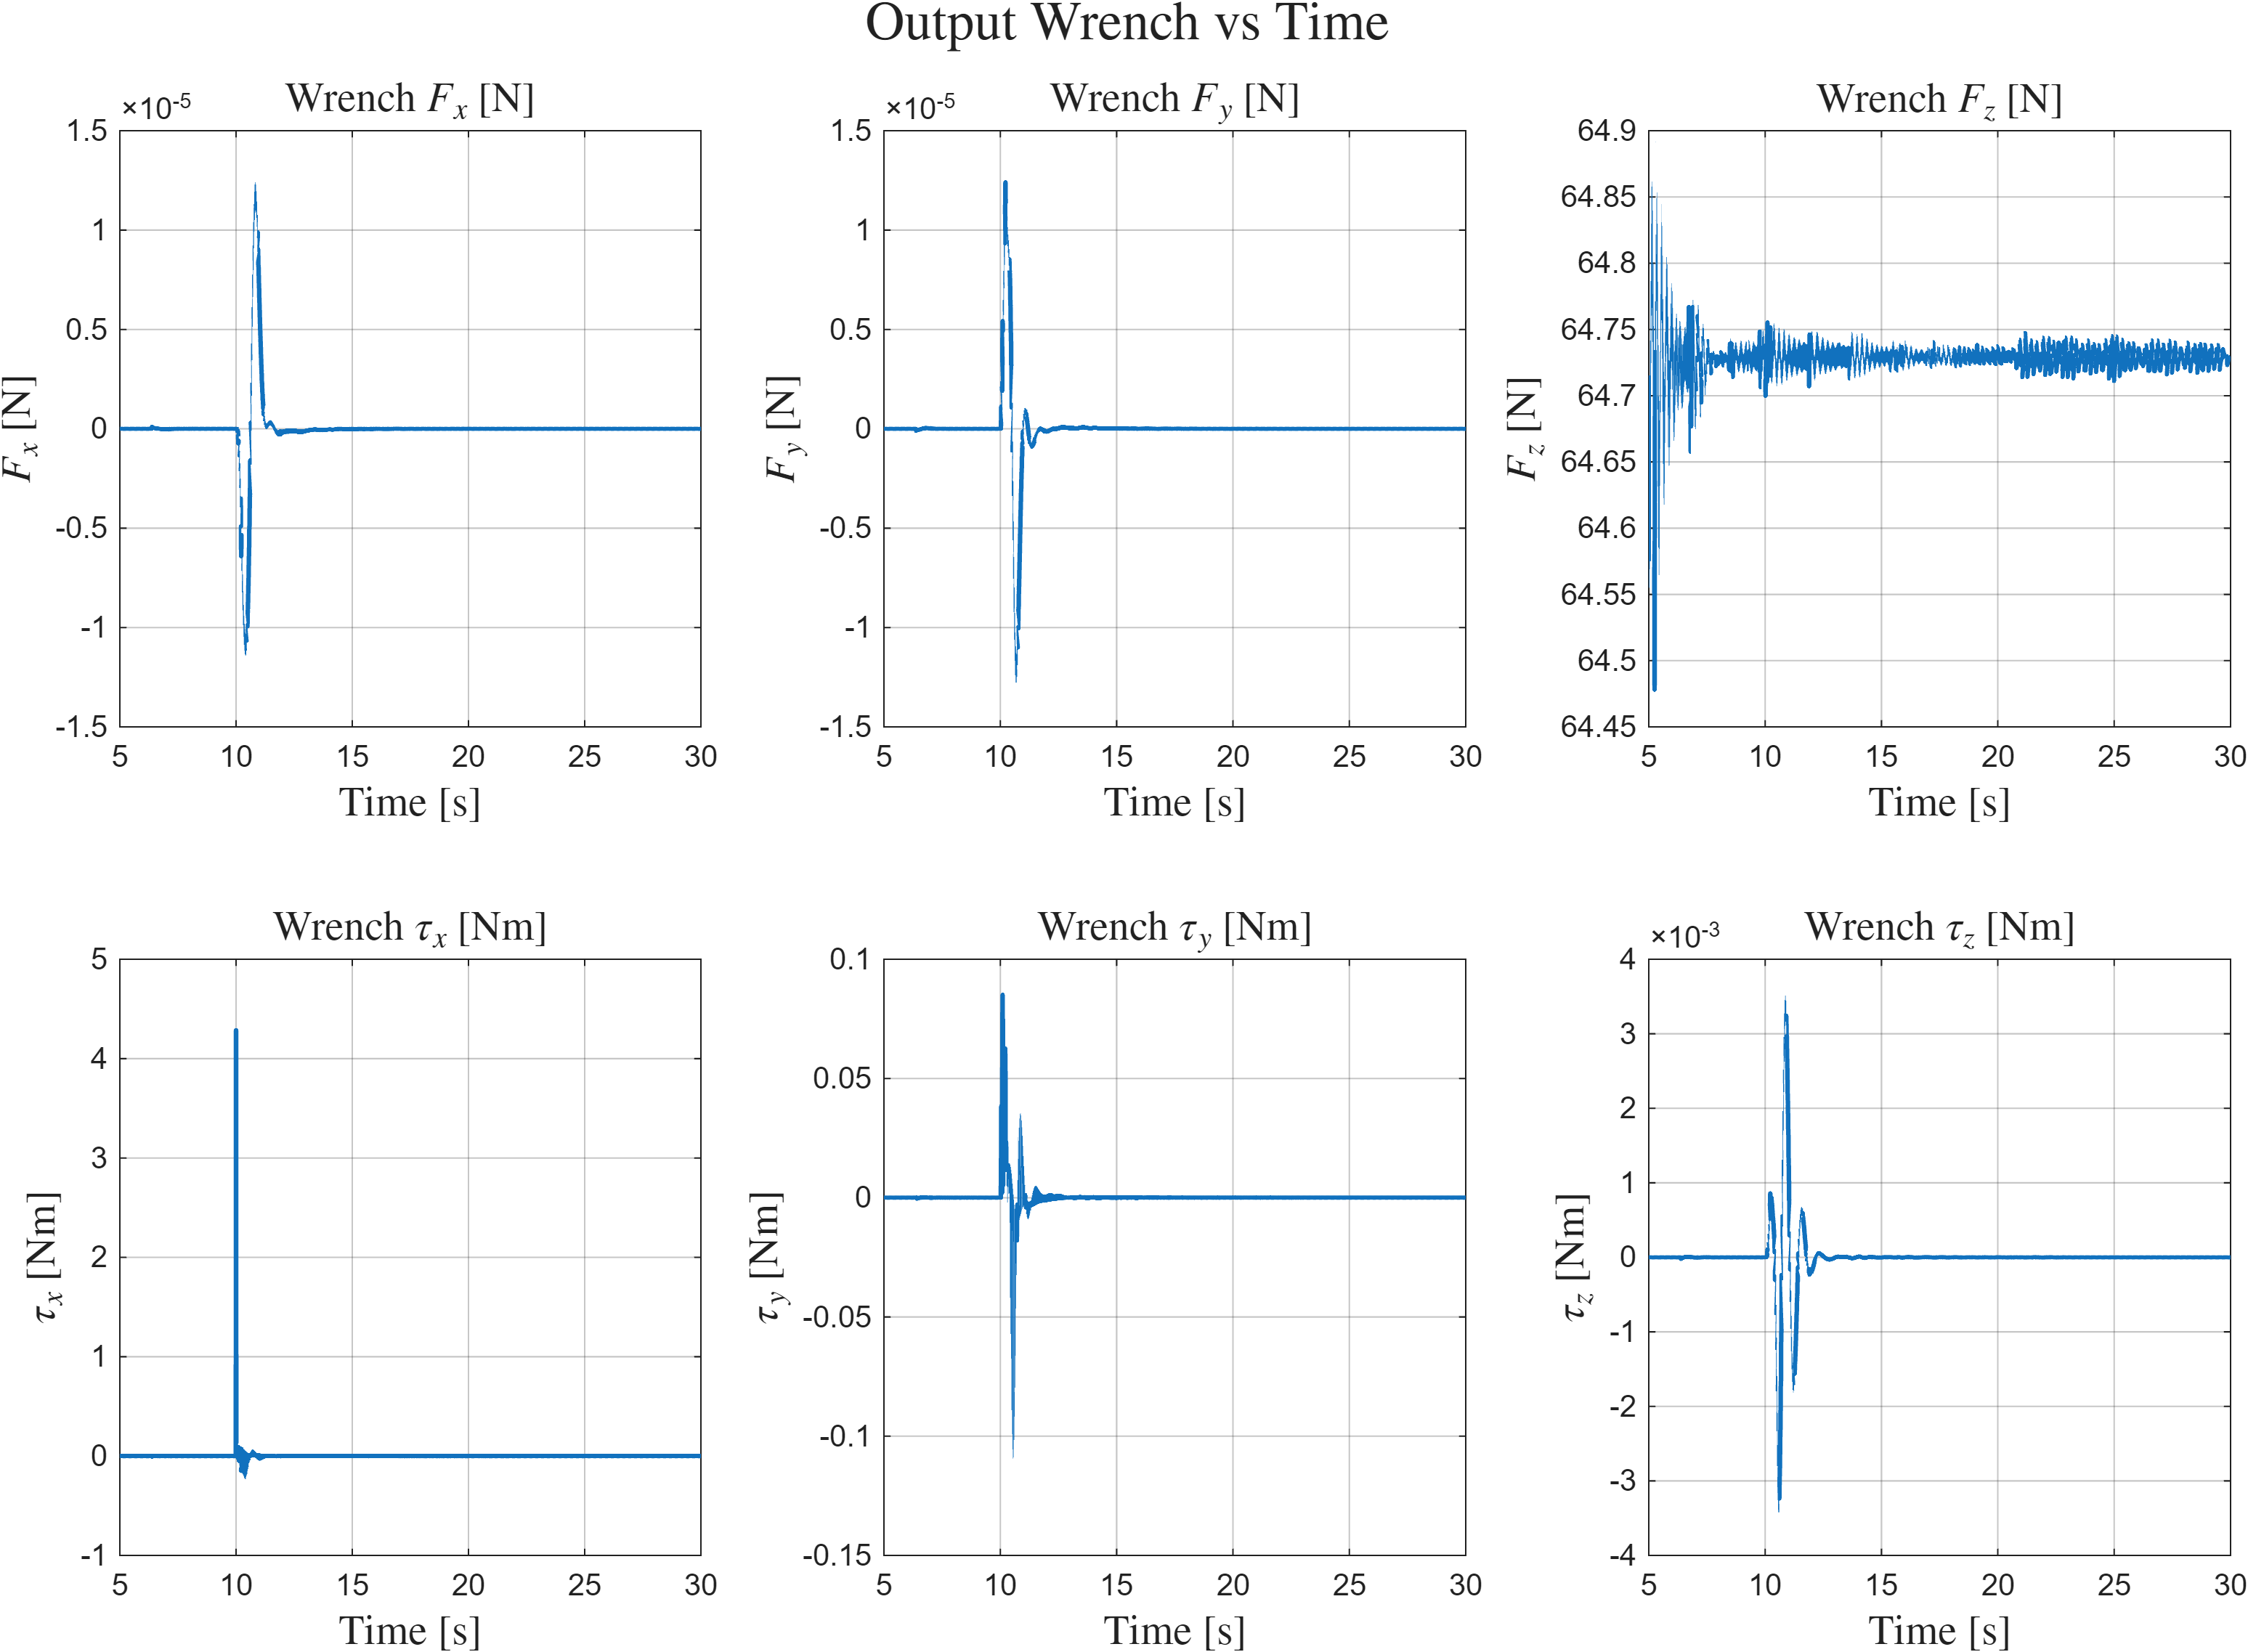
\includegraphics[width=0.48\textwidth]{img/step/alpha/output_wrench}}
	\hfill
	\subfloat[$\beta$]{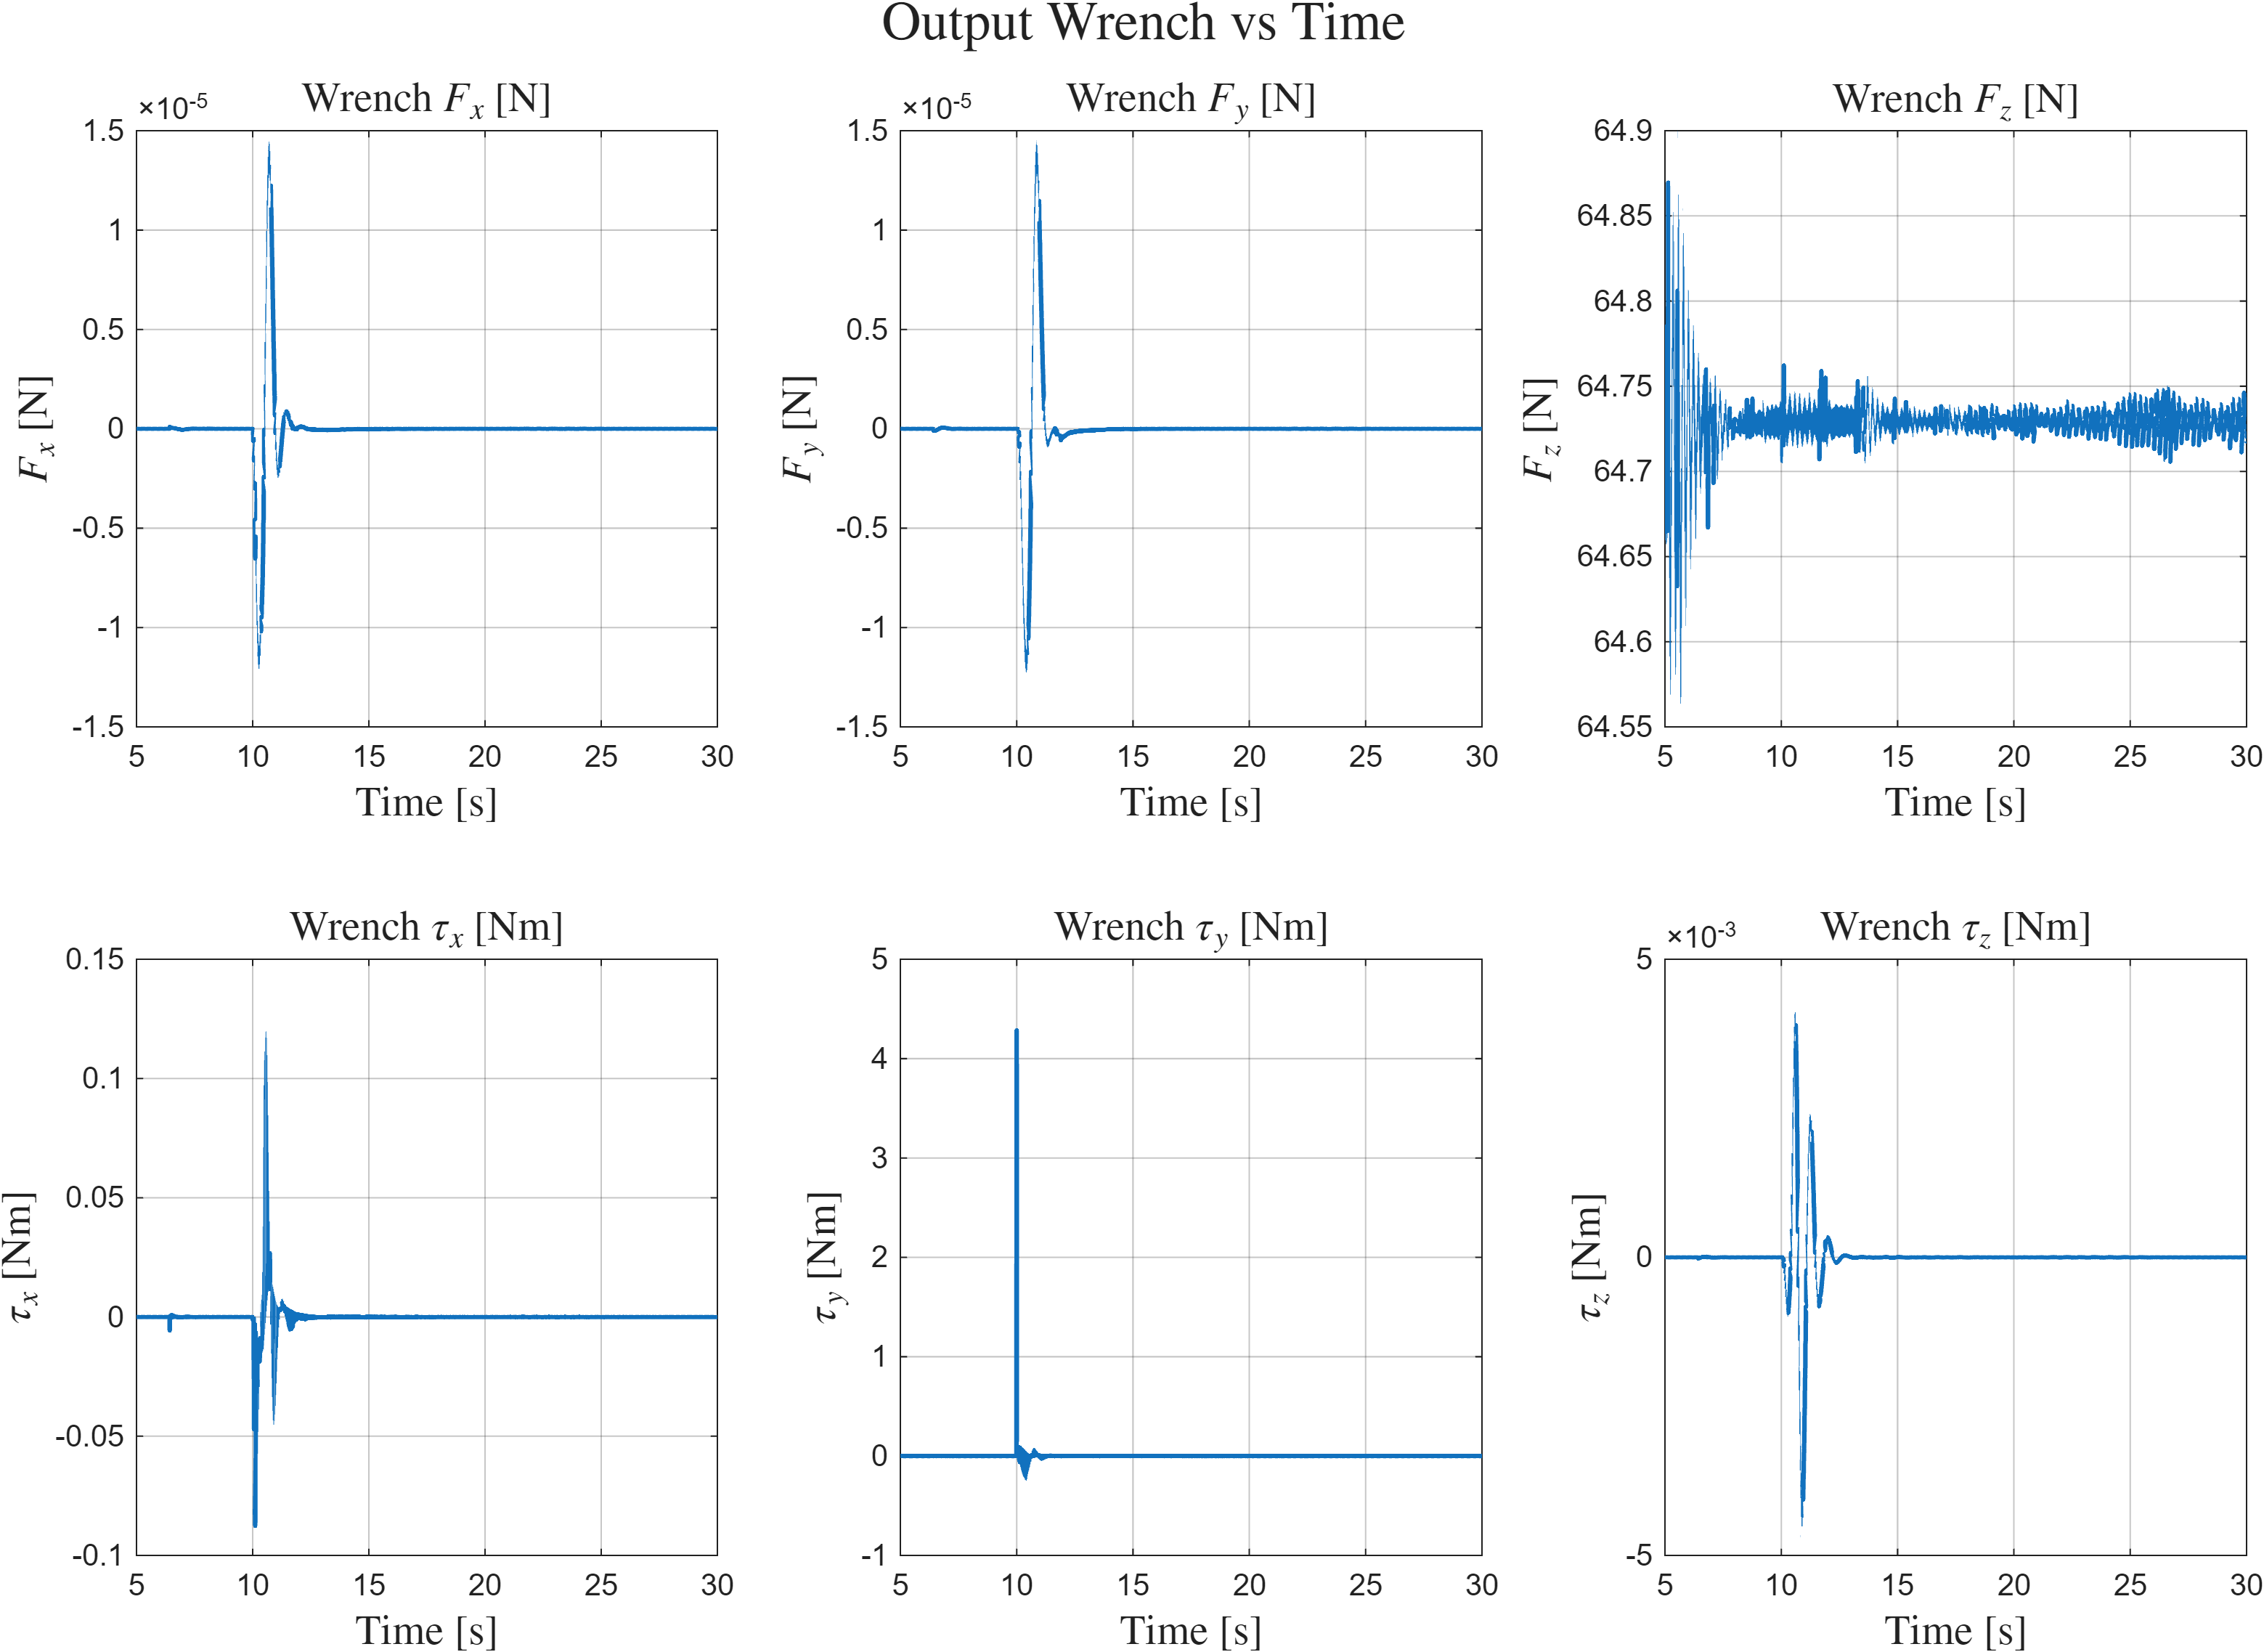
\includegraphics[width=0.48\textwidth]{img/step/beta/output_wrench}}
	
	\caption{پیچش خروجی در درجات آزادی زاویه‌ای $\alpha$ و $\beta$}
	\label{fig:results-wrench-alpha-beta}
\end{figure}

\begin{figure}[htbp]
	\centering
	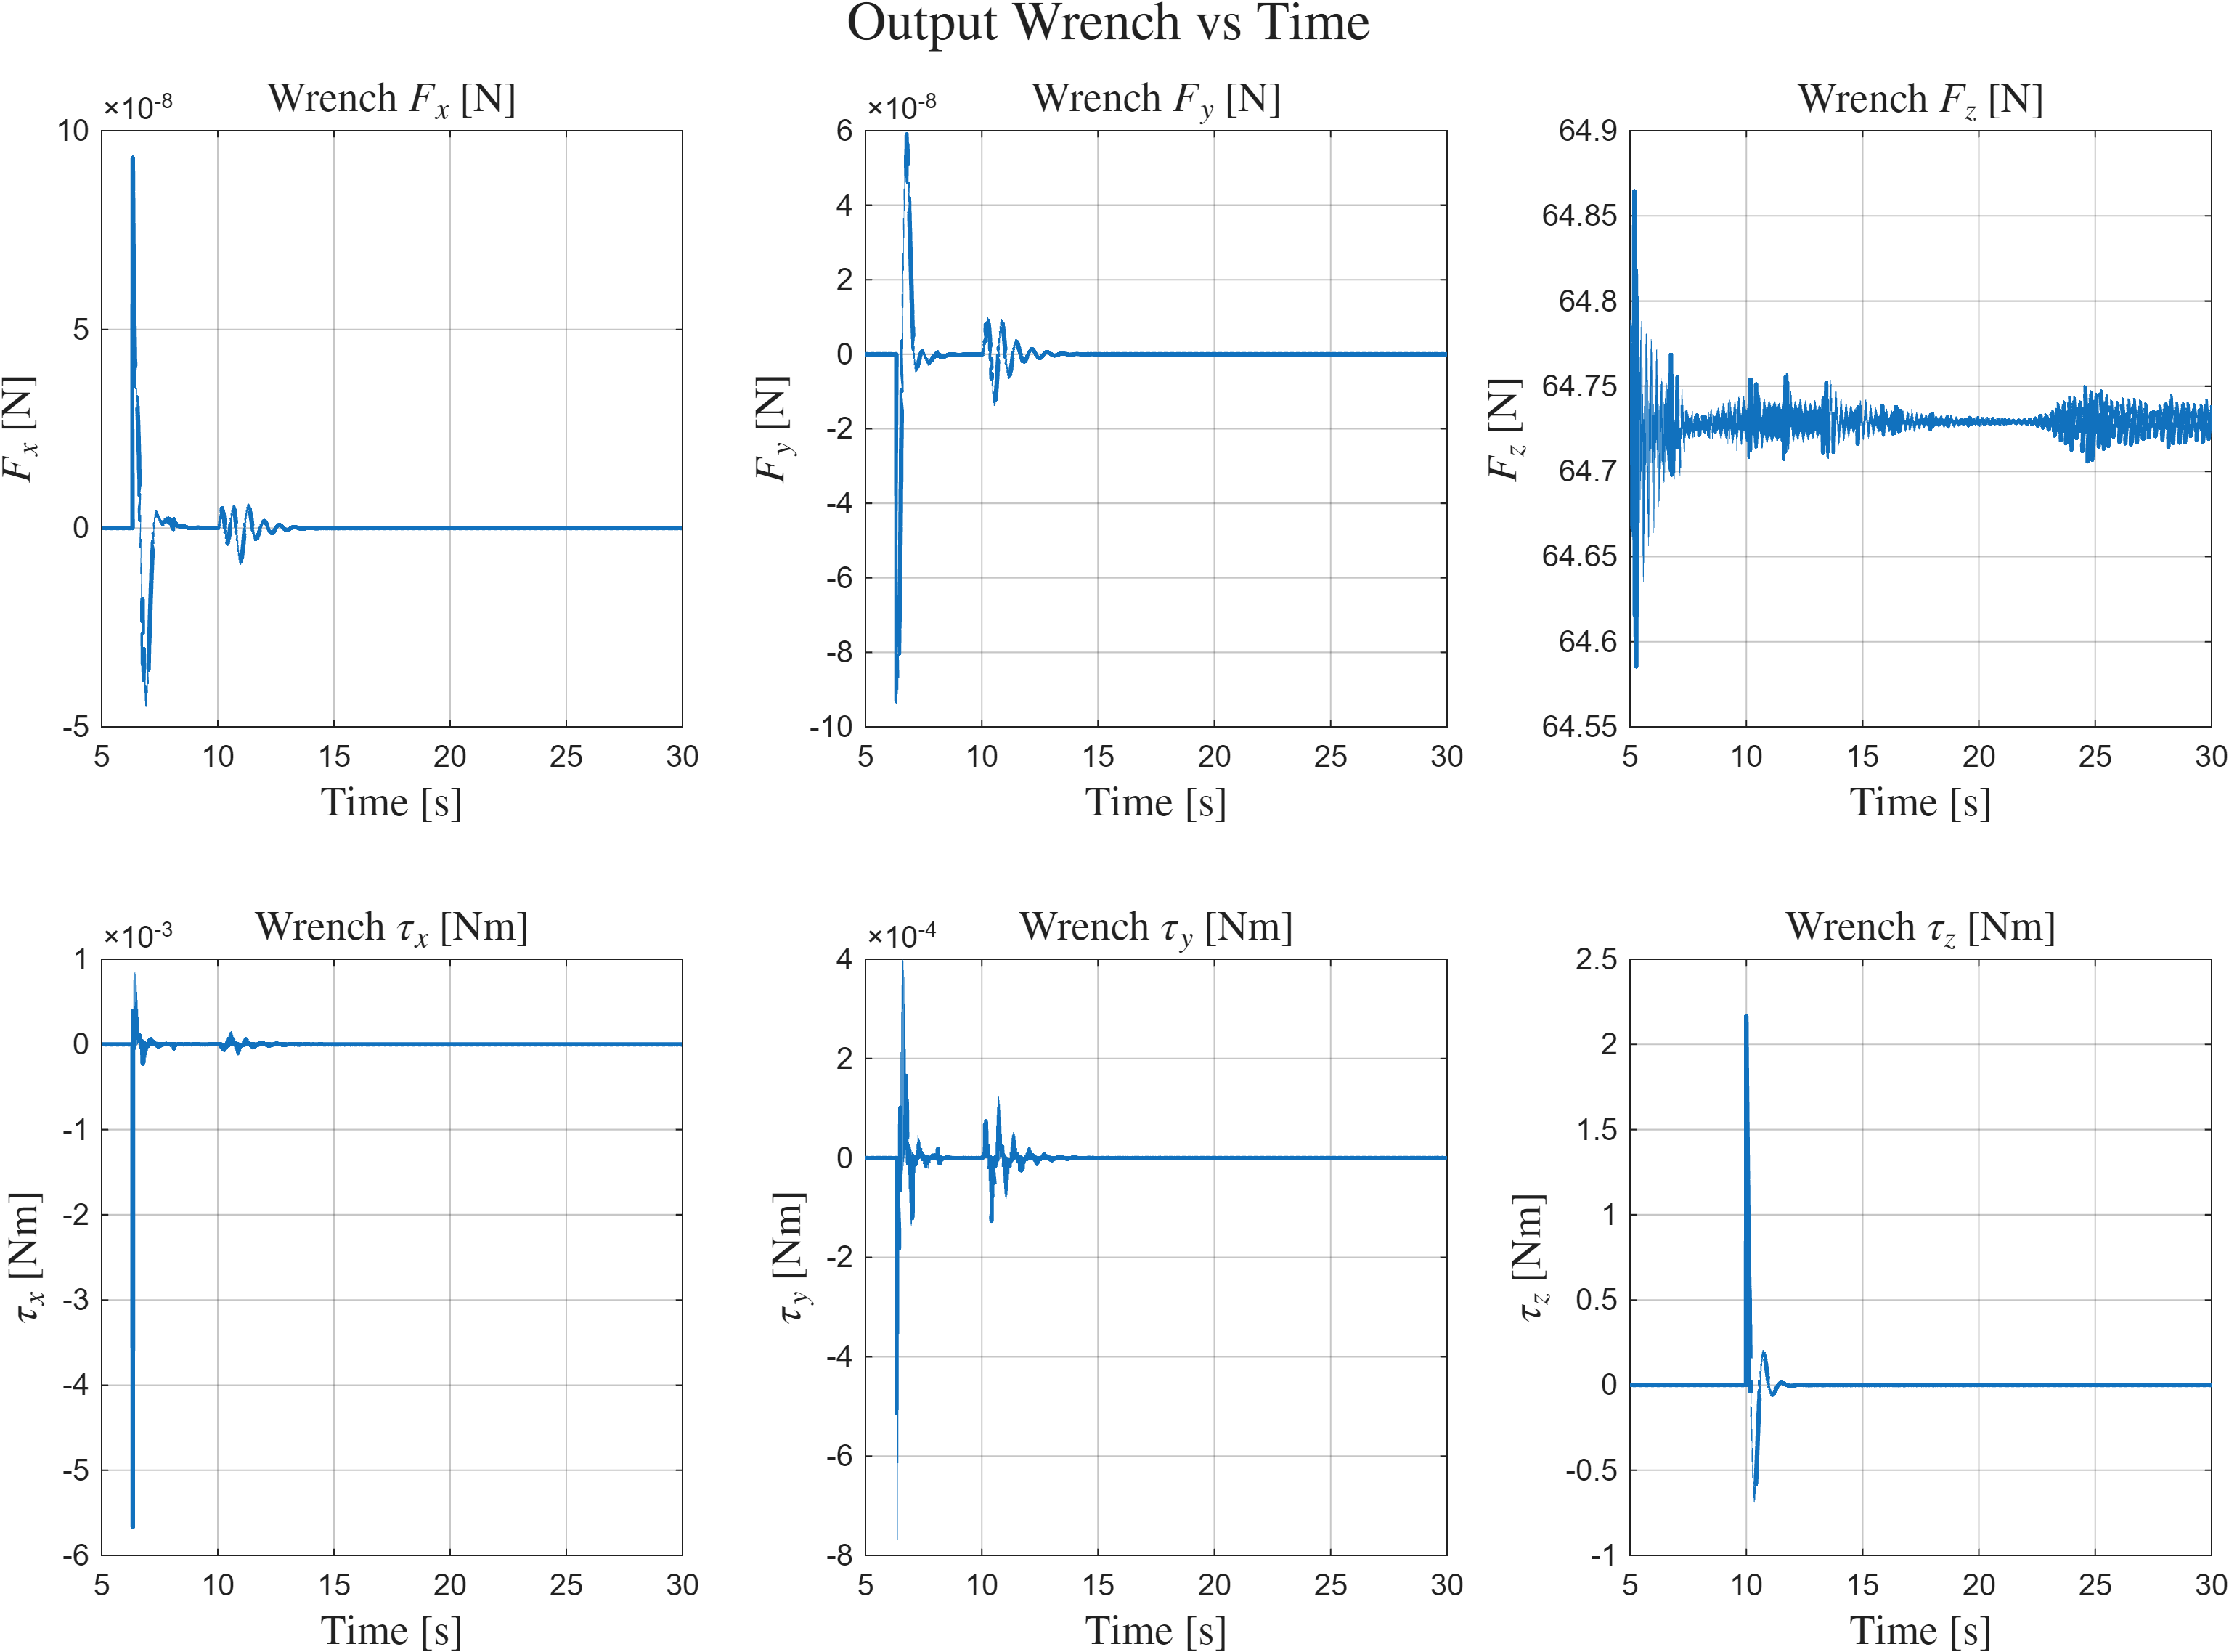
\includegraphics[width=0.75\textwidth]{img/step/gamma/output_wrench}
	\caption{پیچش خروجی در درجه آزادی $\gamma$}
	\label{fig:results-wrench-gamma}
\end{figure}

\section{نتایج تحلیل تکینگی سینماتیکی}
\label{sec:results-singularity}

در این بخش، نتایج عددی حاصل از جستجوی شبکه‌ای عدد شرط $\kappa$ بر روی ماتریس $\Gamma$ که در بخش \ref{sec:method-singularity} تشریح شد، ارائه می‌گردد. هدف، شناسایی نواحی ایمن و بحرانی فضای کاری از منظر تکینگی سینماتیکی و همچنین تأیید تجربی پیش‌بینی‌های تحلیلی است.

\subsection{رفتار بحرانی در محور $\gamma$}
\label{subsec:results-sing-gamma}

با توجه به تحلیل ریاضیاتی، محور $\gamma$ مستعد دو نوع تکینگی (فیزیکی در $\pm\pi$ و مدلی ناشی از قطب‌های مماس در $\pm\pi/2$) است. برای ارزیابی این پیش‌بینی، عدد شرط در یک بازه‌ی گسترده از زوایای $\gamma$ (با ثابت نگه‌داشتن سایر درجات آزادی در مقادیر نامی) محاسبه و در شکل \ref{fig:results-cond-gamma} ترسیم شده است.

\begin{figure}[htbp]
	\centering
	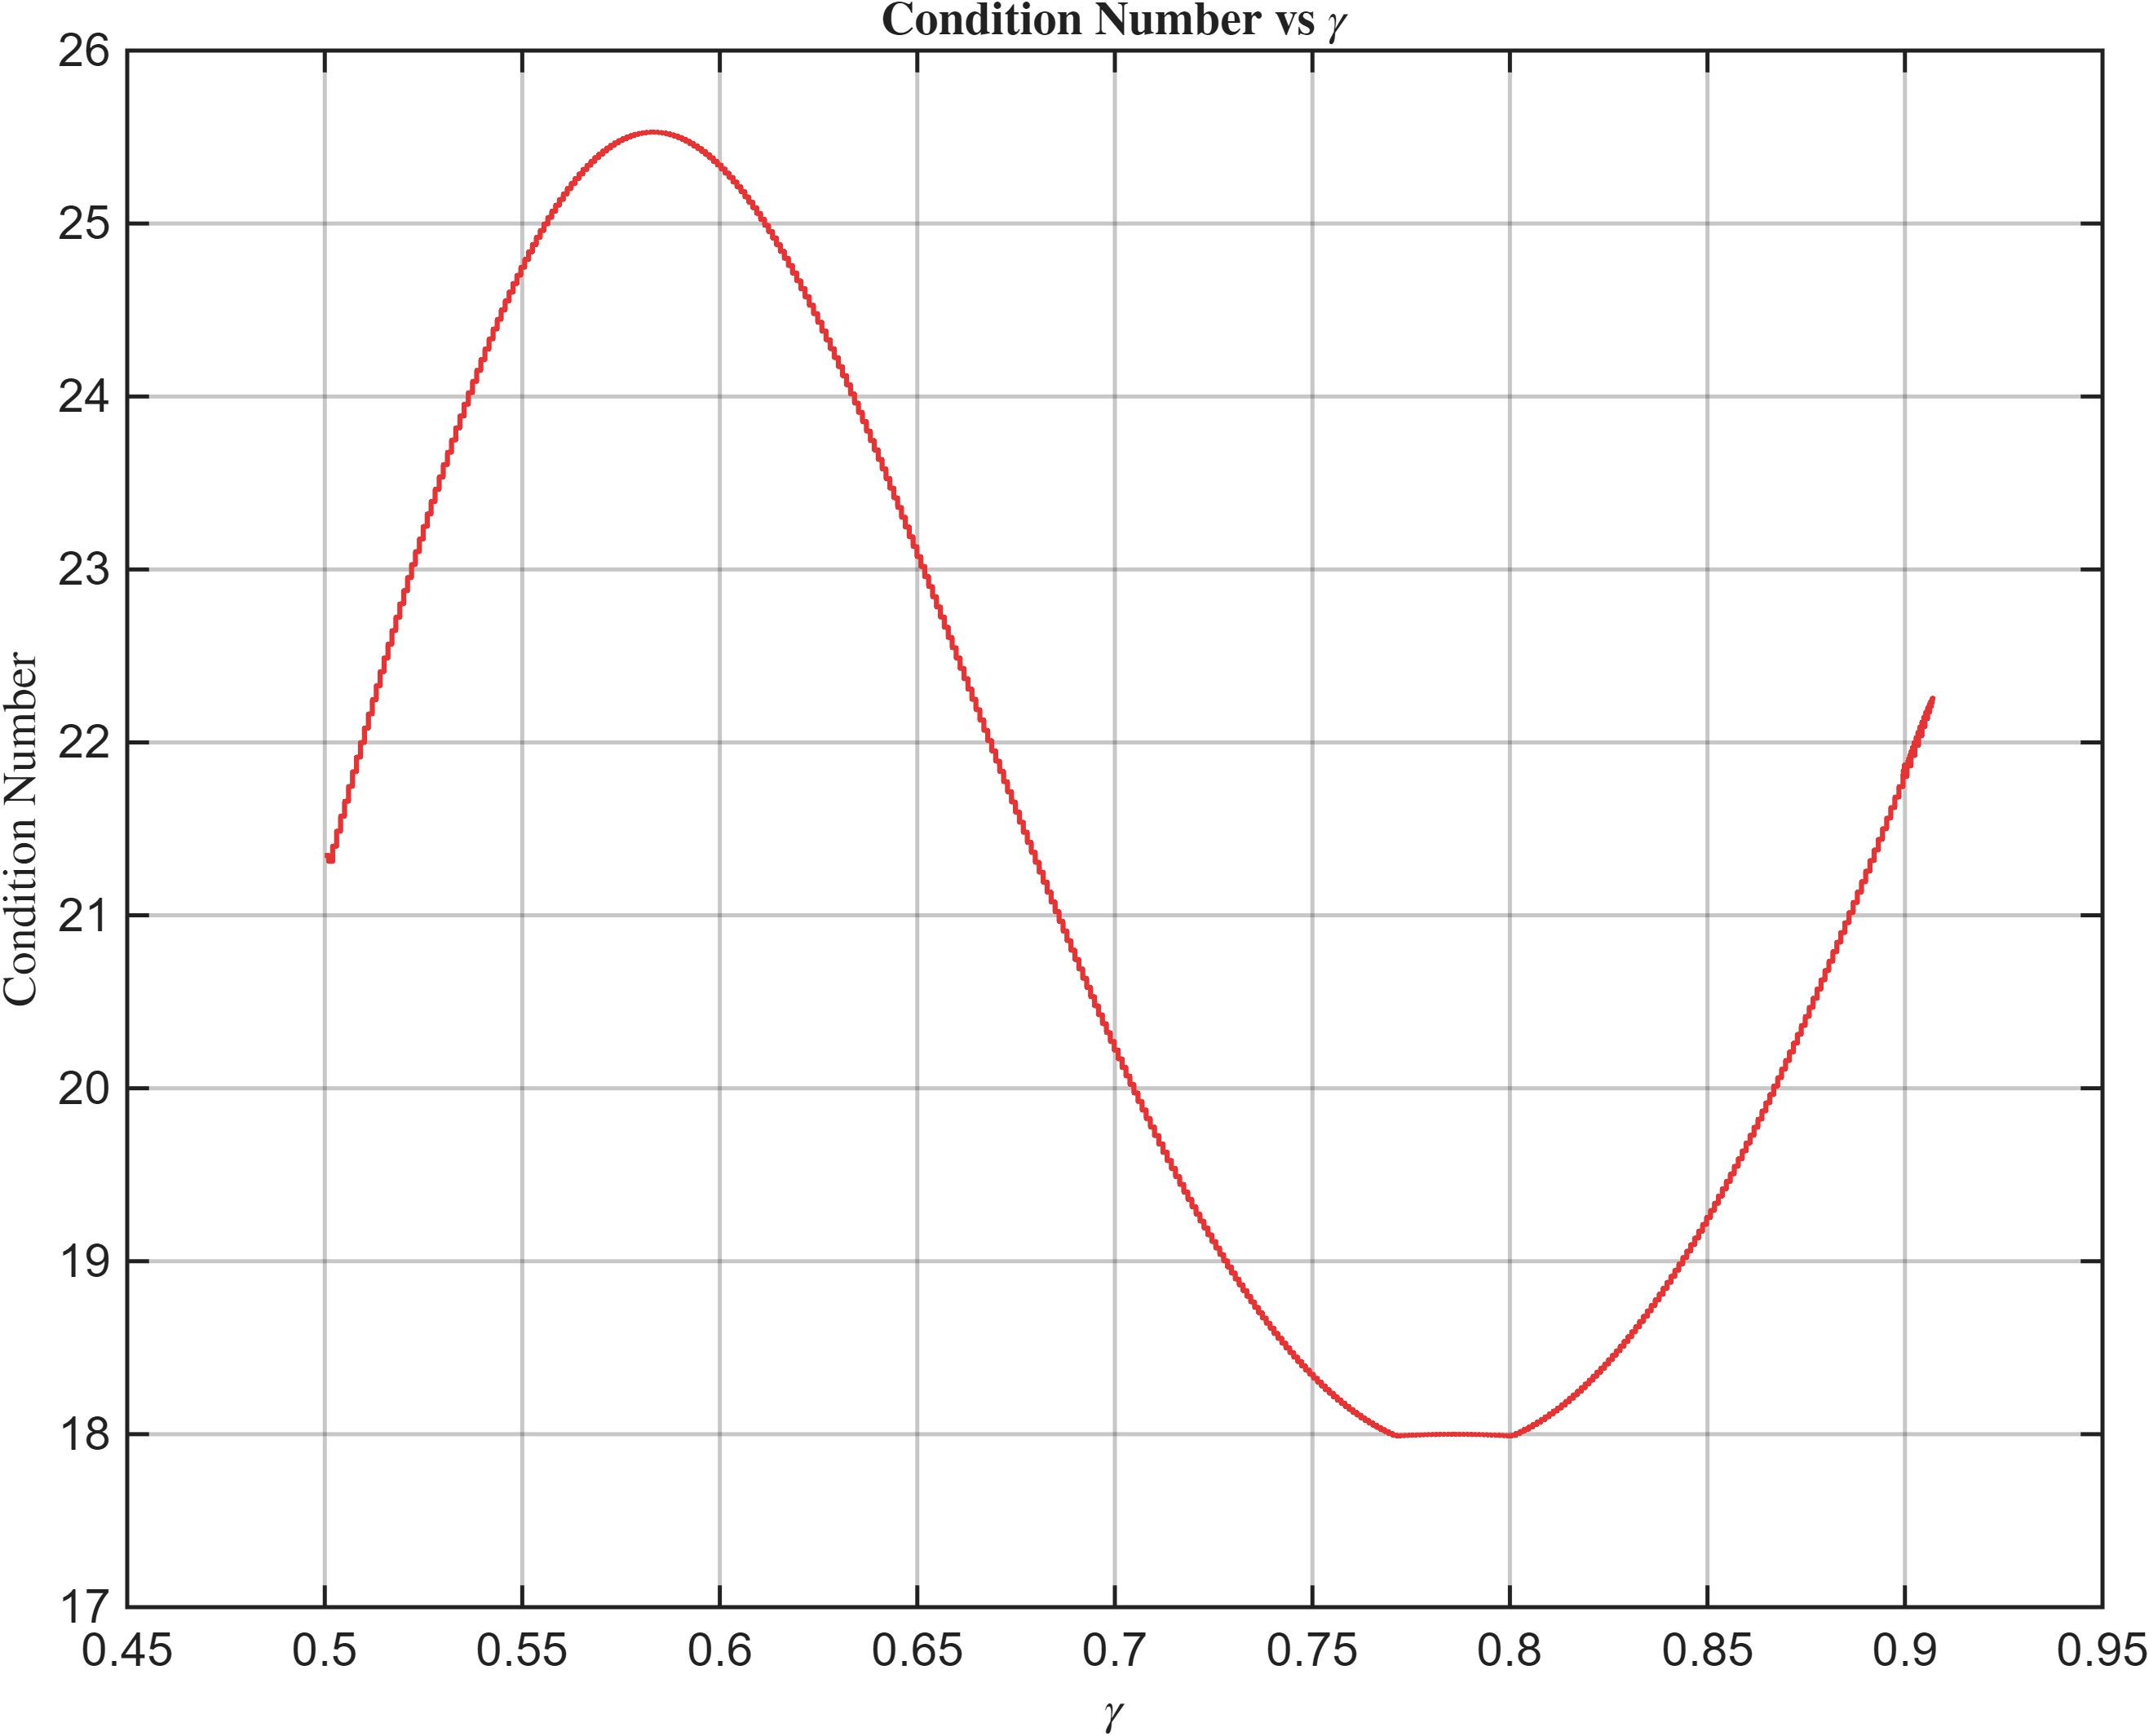
\includegraphics[width=0.75\textwidth]{img/condition_sweep/Pose_condition_gamma/condition_vs_pose_gamma}
	\caption{تغییرات عدد شرط $\kappa$ بر حسب زاویه $\gamma$}
	\label{fig:results-cond-gamma}
\end{figure}

همان‌طور که در شکل \ref{fig:results-cond-gamma} مشاهده می‌شود، عدد شرط در بیشتر نواحی دارای مقادیر بالایی است که نشان‌دهنده‌ی وضعیت نامطلوب سینماتیکی سیستم در این بازه‌ها است. با این حال، یک ناحیه‌ی کاملاً مشخص از کاهش شدید $\kappa$ در اطراف $\gamma = \pi/4$ (معادل عددی $0.7854$ رادیان) دیده می‌شود. در این ناحیه، عدد شرط به کمینه‌ی خود یعنی $18$ می‌رسد که پایین‌ترین مقدار مشاهده‌شده در سراسر فضای کاری است. محدوده‌ی ایمن حول این زاویه تقریباً $\pm \pi/16$ رادیان است که در آن $\kappa$ در مقادیر نسبتاً پایینی باقی می‌ماند. در خارج از این محدوده، عدد شرط به سرعت افزایش یافته و سیستم را در آستانه‌ی ناپایداری عددی قرار می‌دهد. این مشاهدات با تحلیل تحلیلی هم‌خوانی کامل دارد: نزدیک شدن به $\gamma = \pm\pi/2$ باعث فعال شدن قطب‌های مماس در مدل بازوی مؤثر و افزایش $\kappa$ می‌شود و نزدیک شدن به $\gamma = \pm\pi$ نیز به دلیل تقارن مخرب میدان هالباخ، $\sigma_{\min}$ را به صفر میل می‌دهد.

\subsection{رفتار عدد شرط در محورهای انتقالی $X$ و $Y$}
\label{subsec:results-sing-xy}

برای ارزیابی سلامت سینماتیکی در صفحه‌ی افقی، عدد شرط در امتداد محورهای $X$ و $Y$ به صورت مجزا محاسبه گردید. در این آزمون، $\gamma$ بر روی مقدار بهینه‌ی $\pi/4$ و $\alpha$ و $\beta$ بر روی صفر تنظیم شدند. نتایج برای محور $X$ و $Y$ در شکل \ref{fig:results-cond-xy} نشان داده شده است.

\begin{figure}[htbp]
	\centering
	\subfloat[محور $X$]{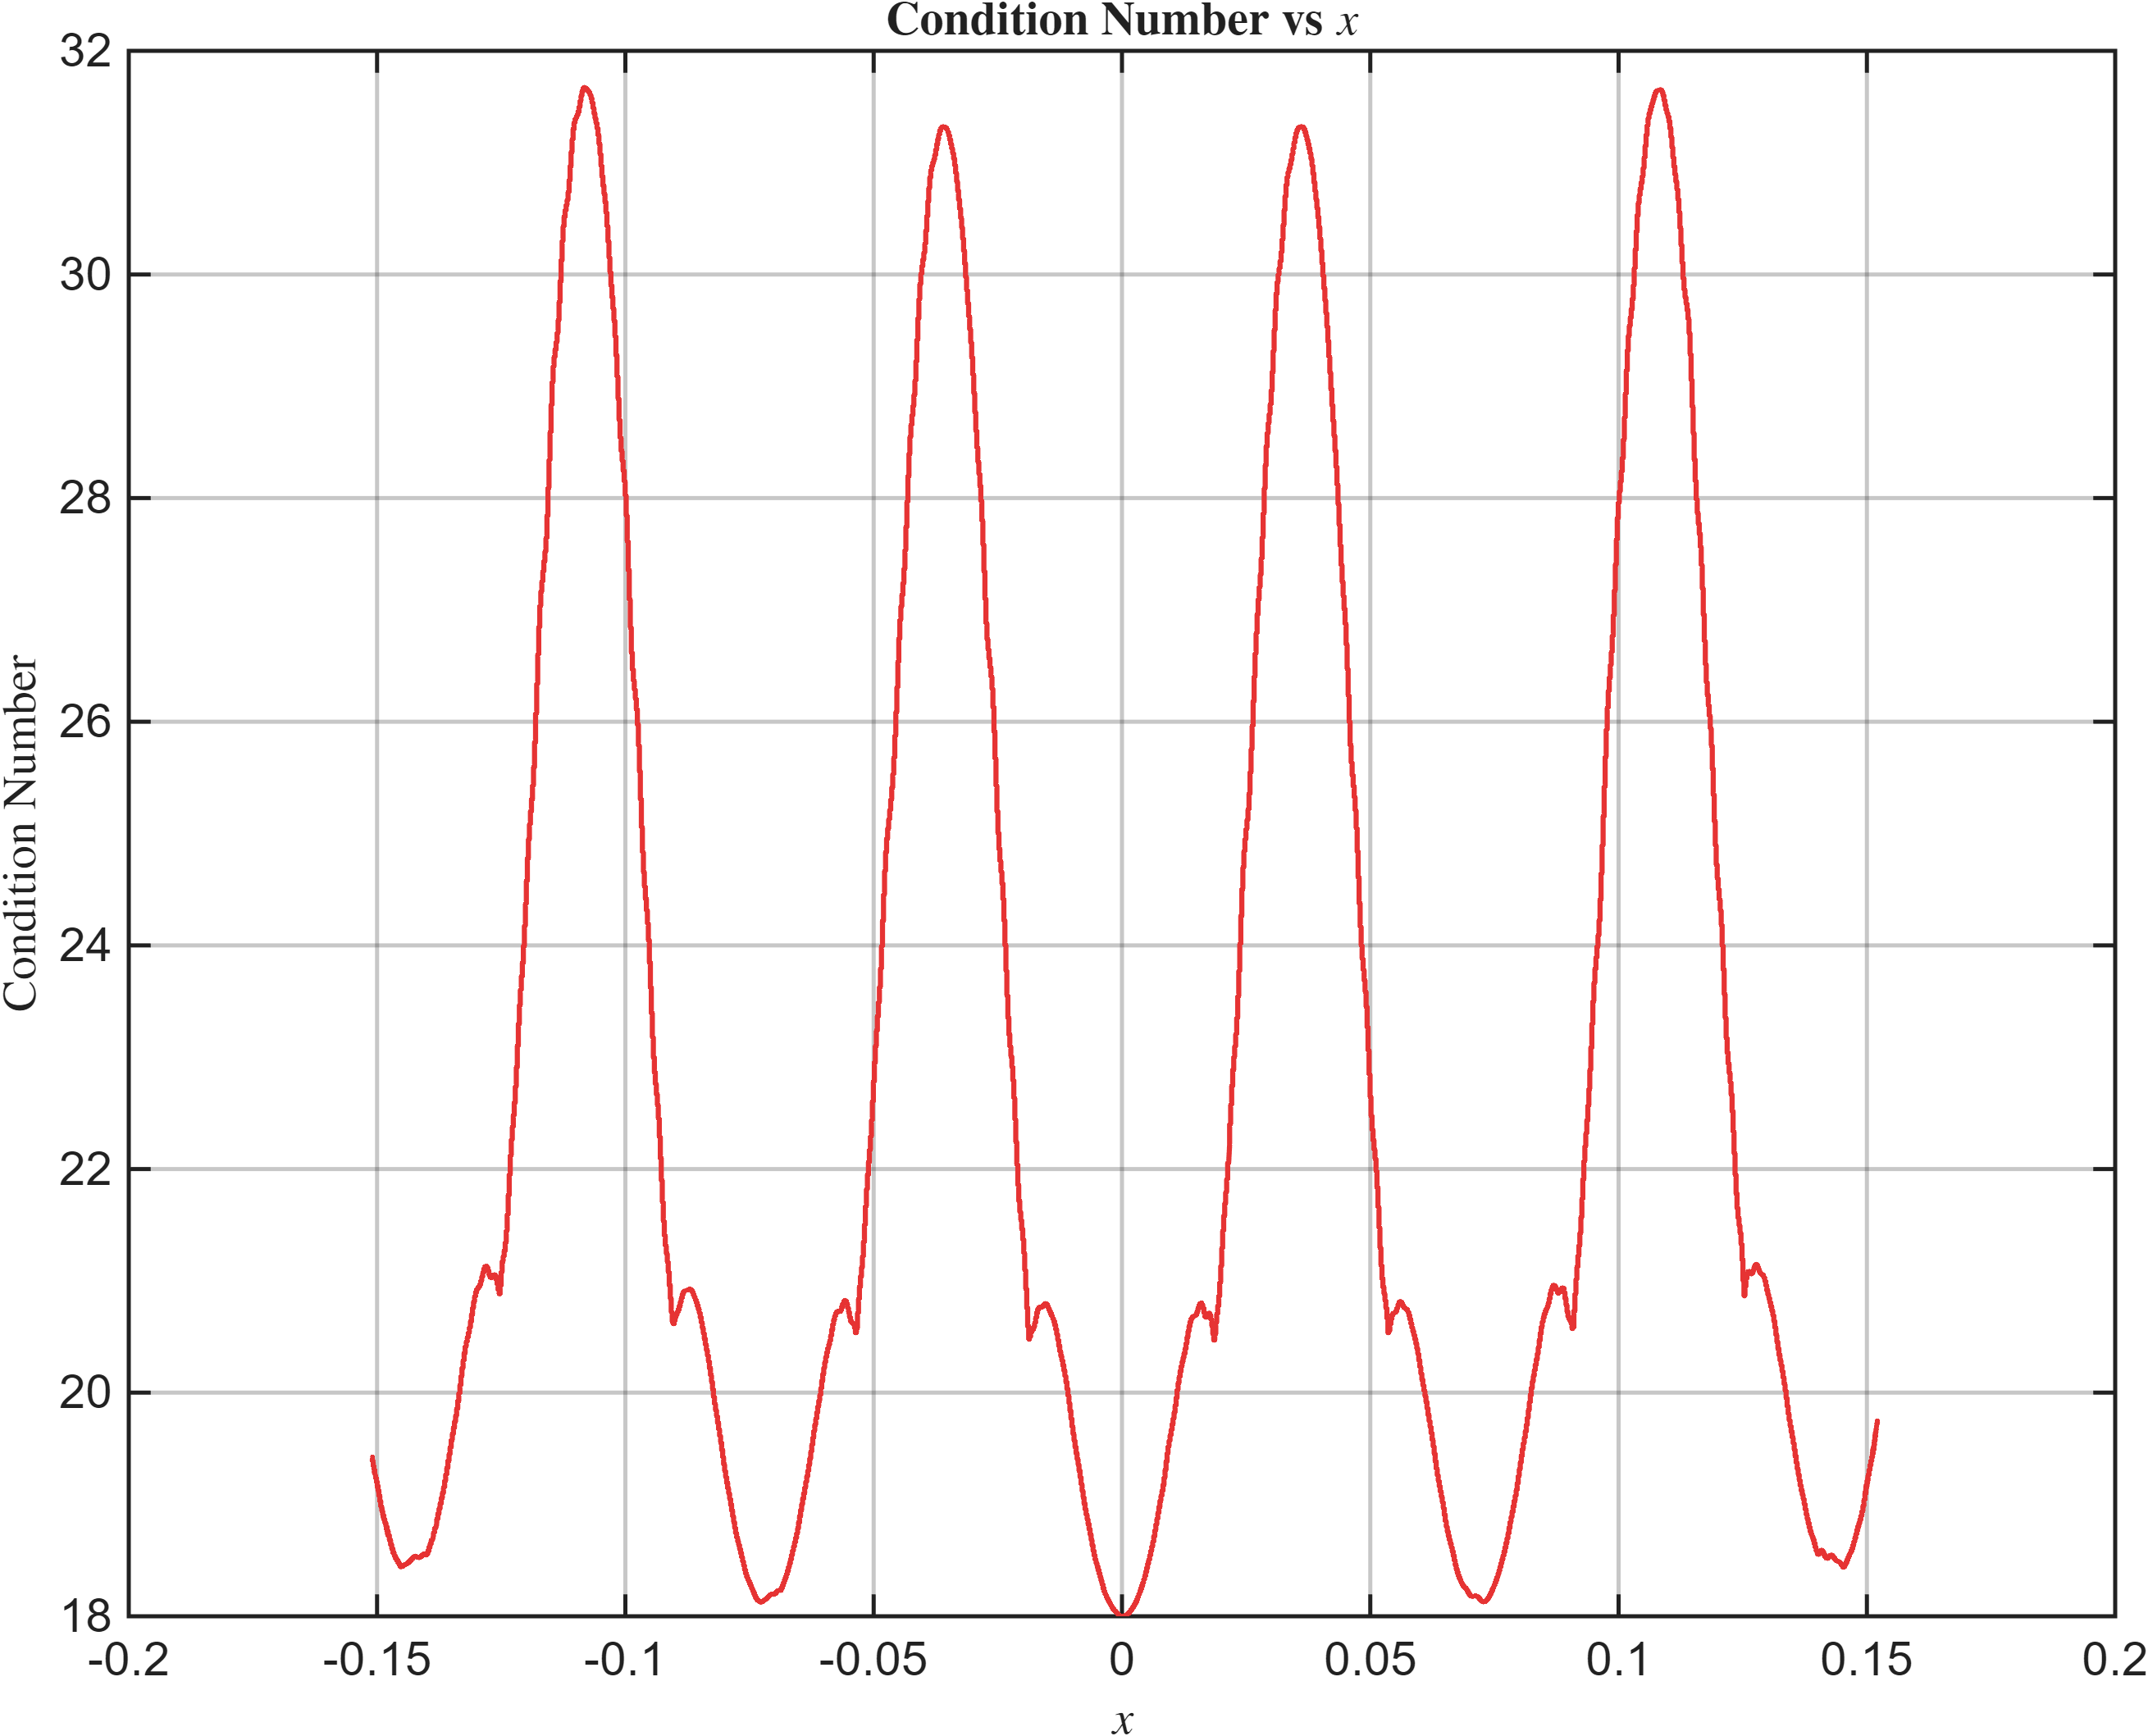
\includegraphics[width=0.48\textwidth]{img/condition_sweep/Pose_condition_x/condition_vs_pose_x}}
	\hfill
	\subfloat[محور $Y$]{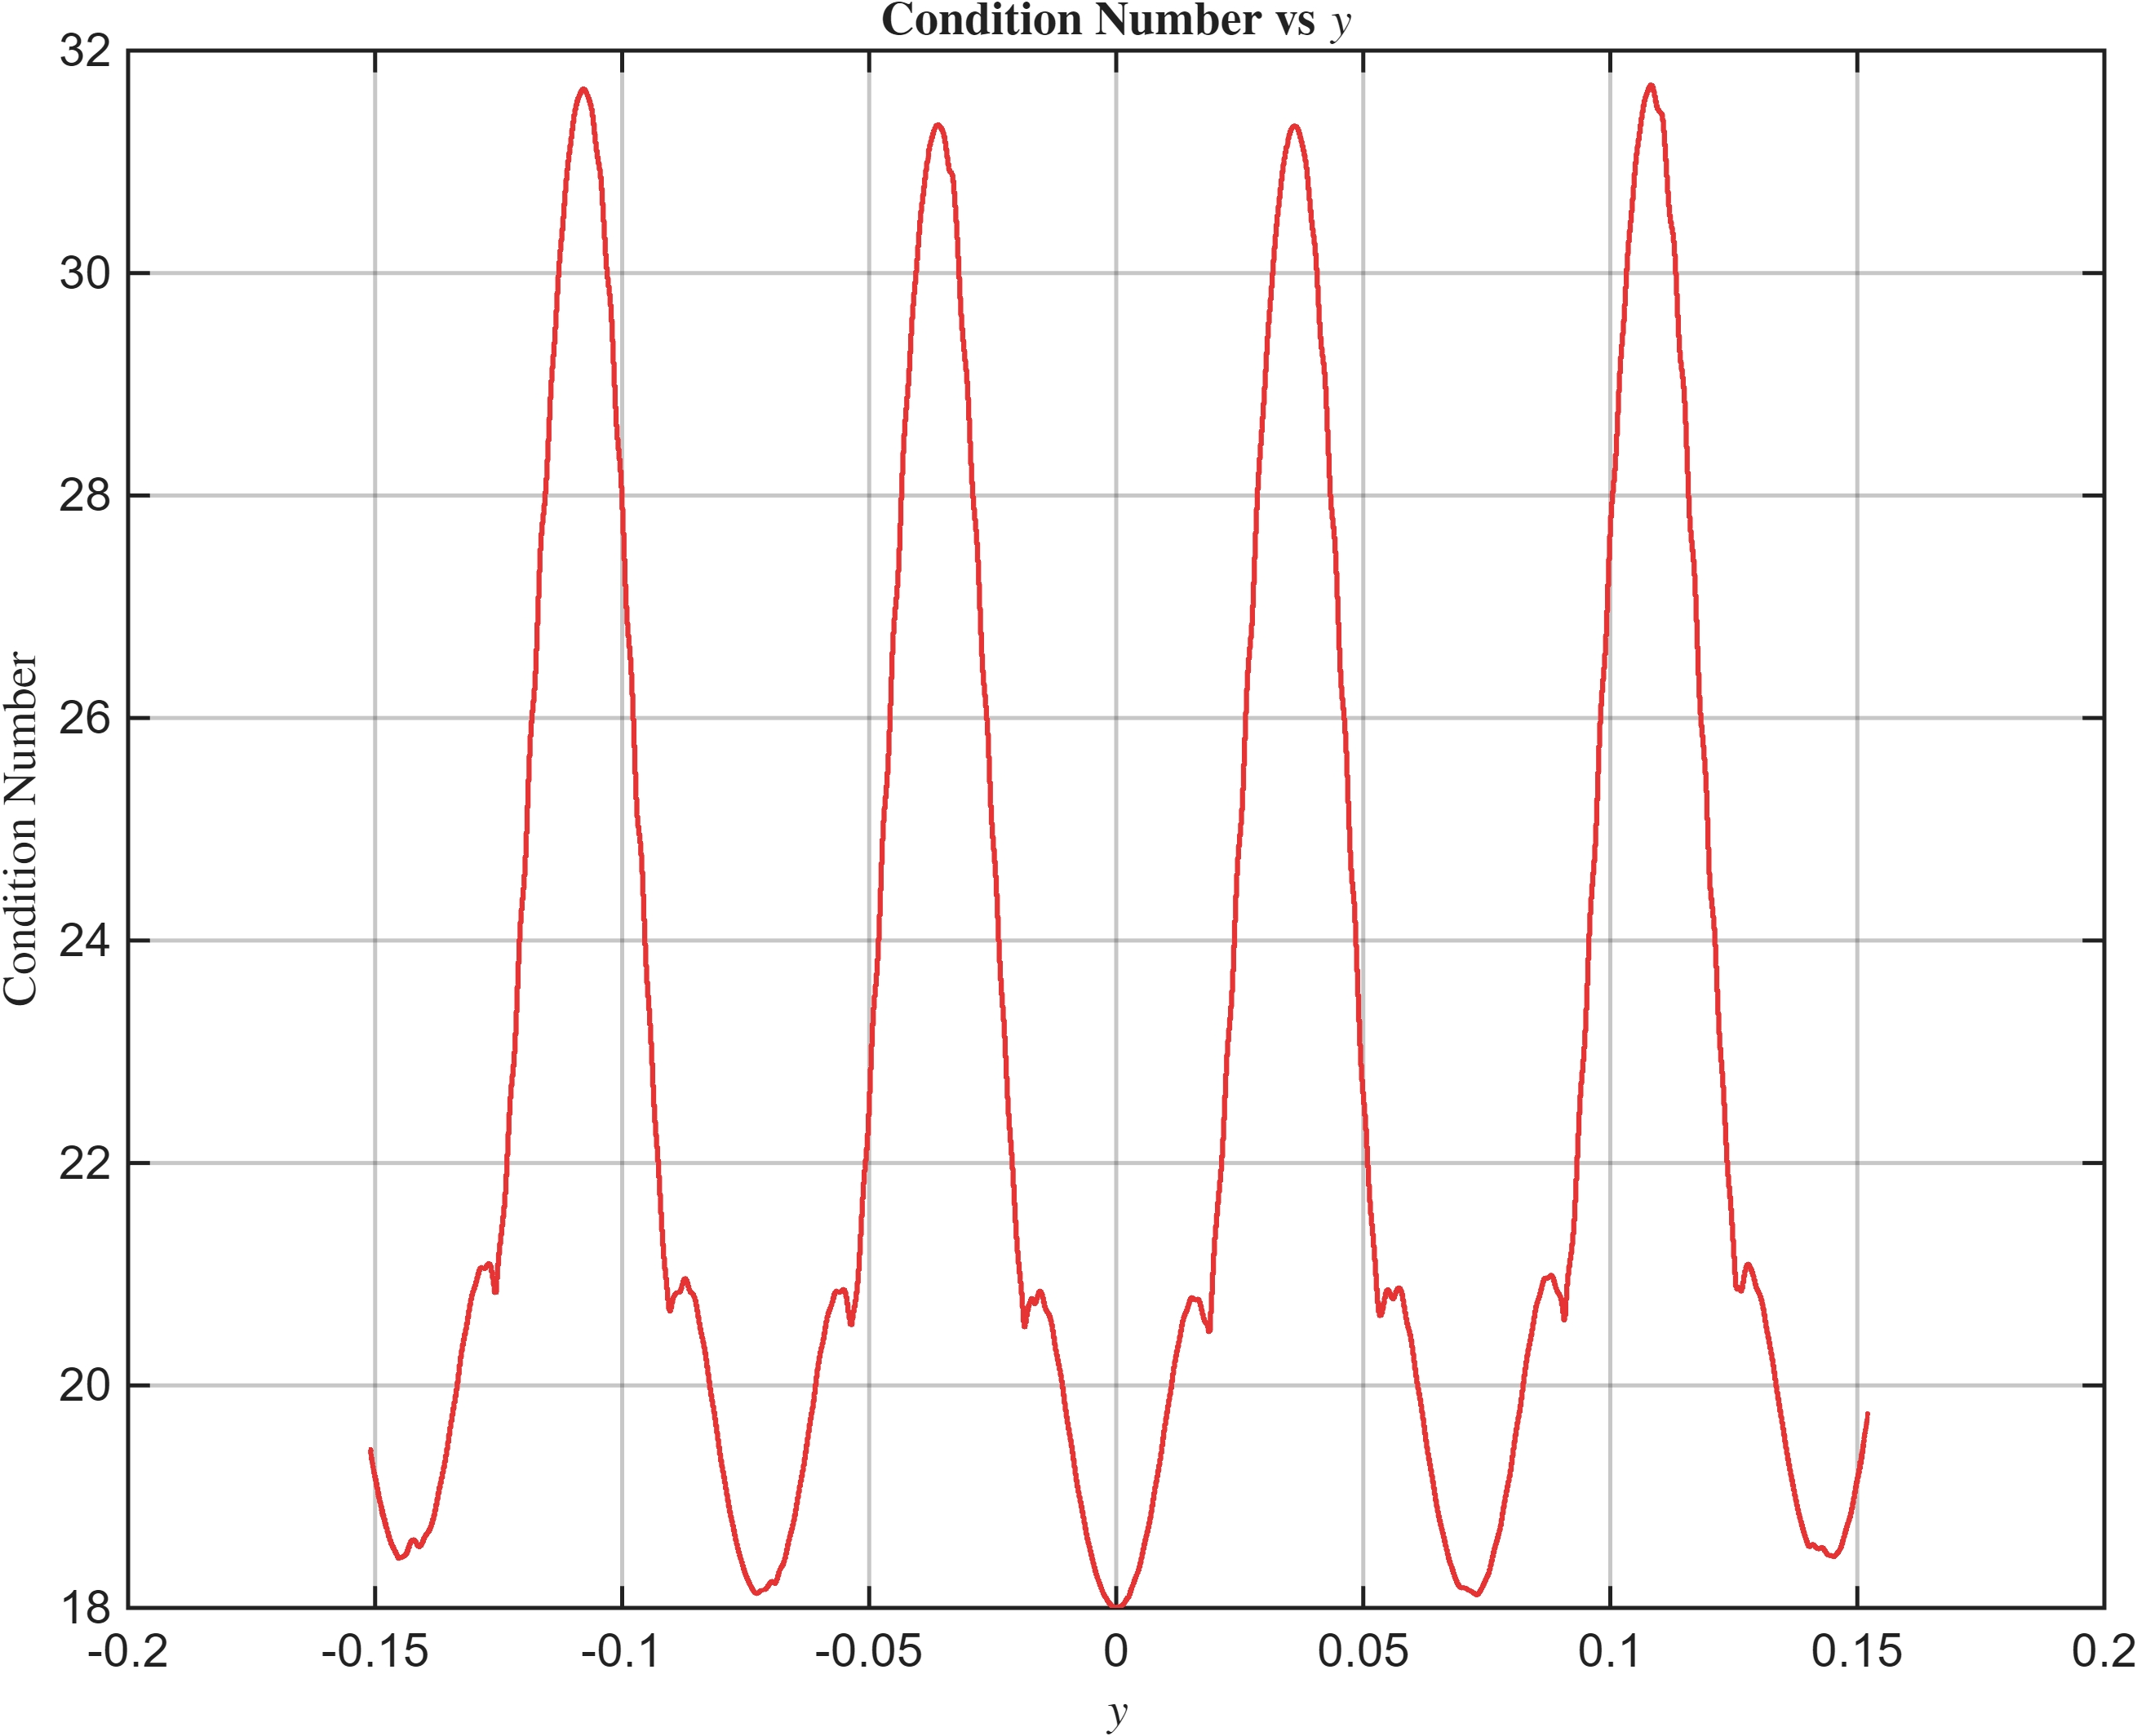
\includegraphics[width=0.48\textwidth]{img/condition_sweep/Pose_condition_y/condition_vs_pose_y}}
	\caption{تغییرات عدد شرط $\kappa$ در محورهای انتقالی $X$ و $Y$}
	\label{fig:results-cond-xy}
\end{figure}

همان‌طور که در شکل \ref{fig:results-cond-xy} دیده می‌شود، عدد شرط در هر دو محور یک رفتار سینوسی از خود نشان می‌دهد. این نوسان، بازتاب مستقیم ساختار تناوبی میدان مغناطیسی تولیدشده توسط چینش آهنرباهای آرایه‌ی هالباخ و آرایش سیم‌پیچ‌ها است. با حرکت بخش متحرک در صفحه، موقعیت نسبی سیم‌پیچ‌ها نسبت به قطب‌های مغناطیسی تغییر کرده و در نتیجه، میزان استقلال بردارهای پیچش (ستون‌های $\Gamma$) به صورت متناوب کم و زیاد می‌شود. نکته‌ی حائز اهمیت آن است که دامنه‌ی این نوسان کاملاً محدود است: عدد شرط در بهترین نقاط به $18$ و در بدترین نقاط به $34$ می‌رسد. این مقادیر، با توجه به معیارهای پذیرفته‌شده در رباتیک، کاملاً ایمن بوده و نشان‌دهنده‌ی یک فضای کاری خوش‌حالت برای حرکات صفحه‌ای است.

\subsection{تأثیر زوایای $\alpha$ و $\beta$ بر عدد شرط}
\label{subsec:results-sing-alpha-beta}

در نهایت، حساسیت عدد شرط به زوایای رول و پیچ ($\alpha$ و $\beta$) مورد بررسی قرار گرفت. جستجو در بازه‌ی $\pm 3$ درجه ($\pm 0.052$ رادیان) برای هر یک از این زوایا (با ثابت نگه‌داشتن $\gamma$ در $\pi/4$) انجام و نتایج در شکل \ref{fig:results-cond-alpha-beta} ارائه شده است.

\begin{figure}[htbp]
	\centering
	\subfloat[محور $\alpha$]{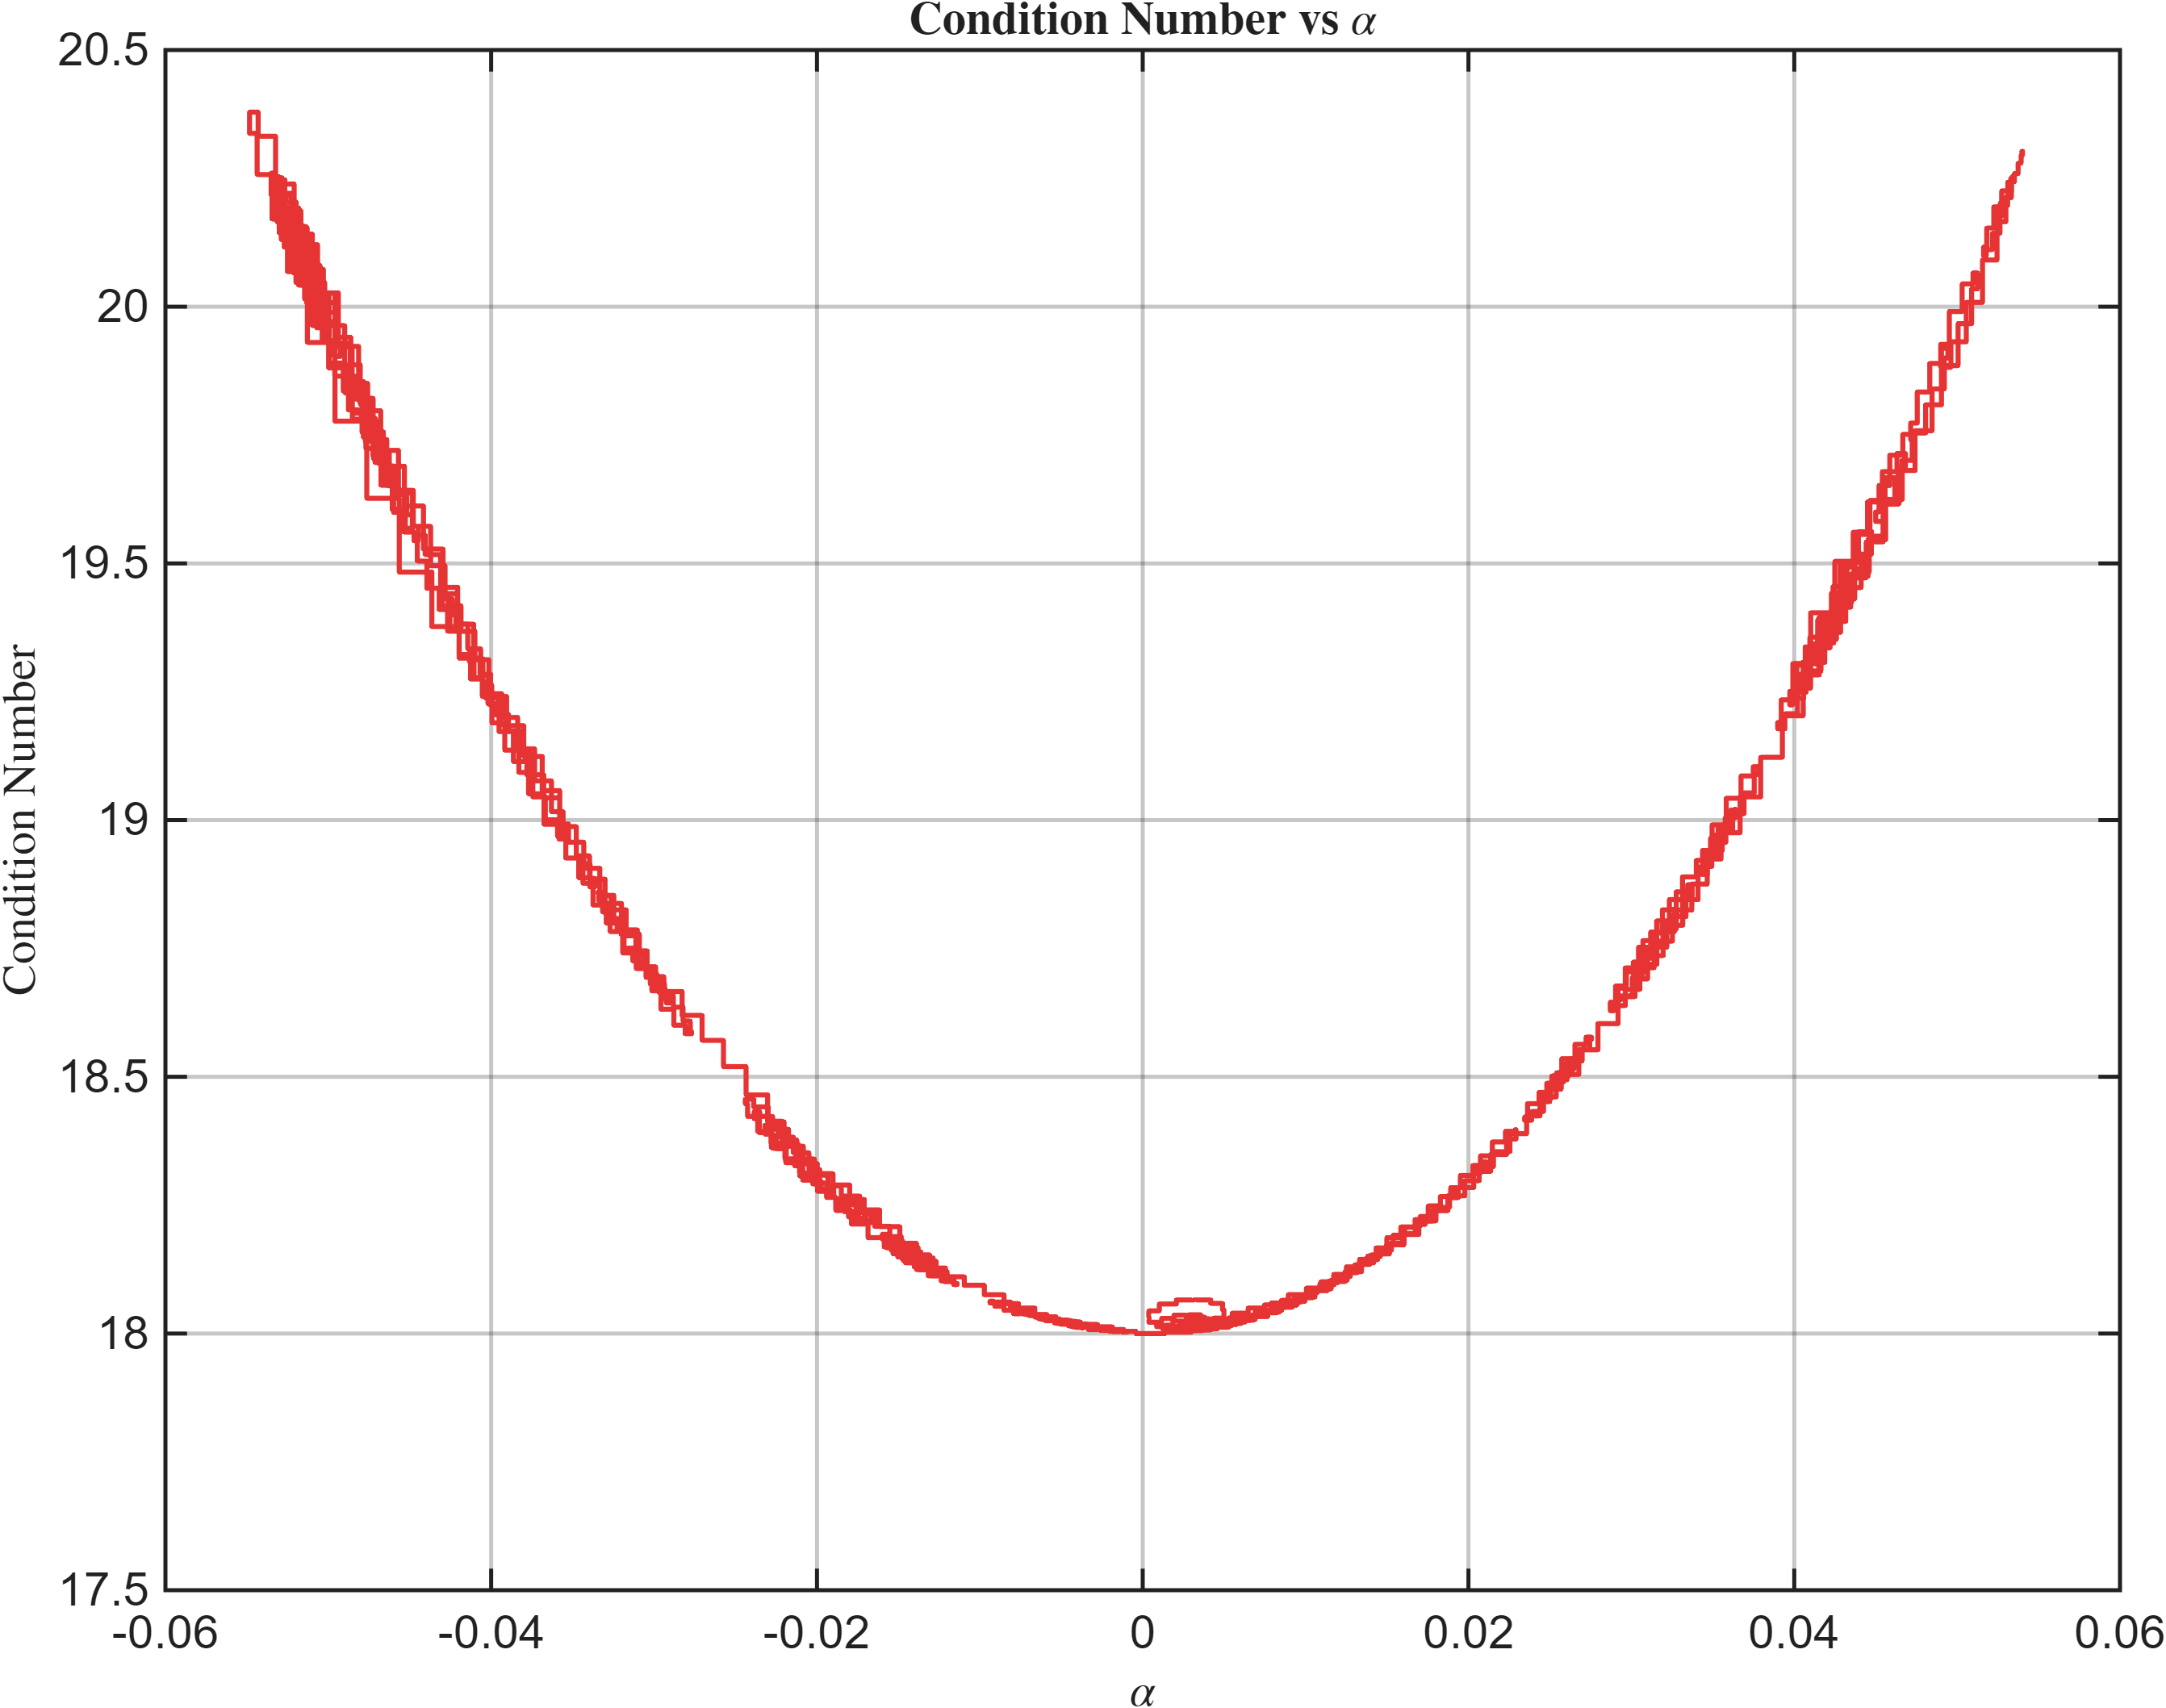
\includegraphics[width=0.48\textwidth]{img/condition_sweep/Pose_condition_alpha/condition_vs_pose_alpha}}
	\hfill
	\subfloat[محور $\beta$]{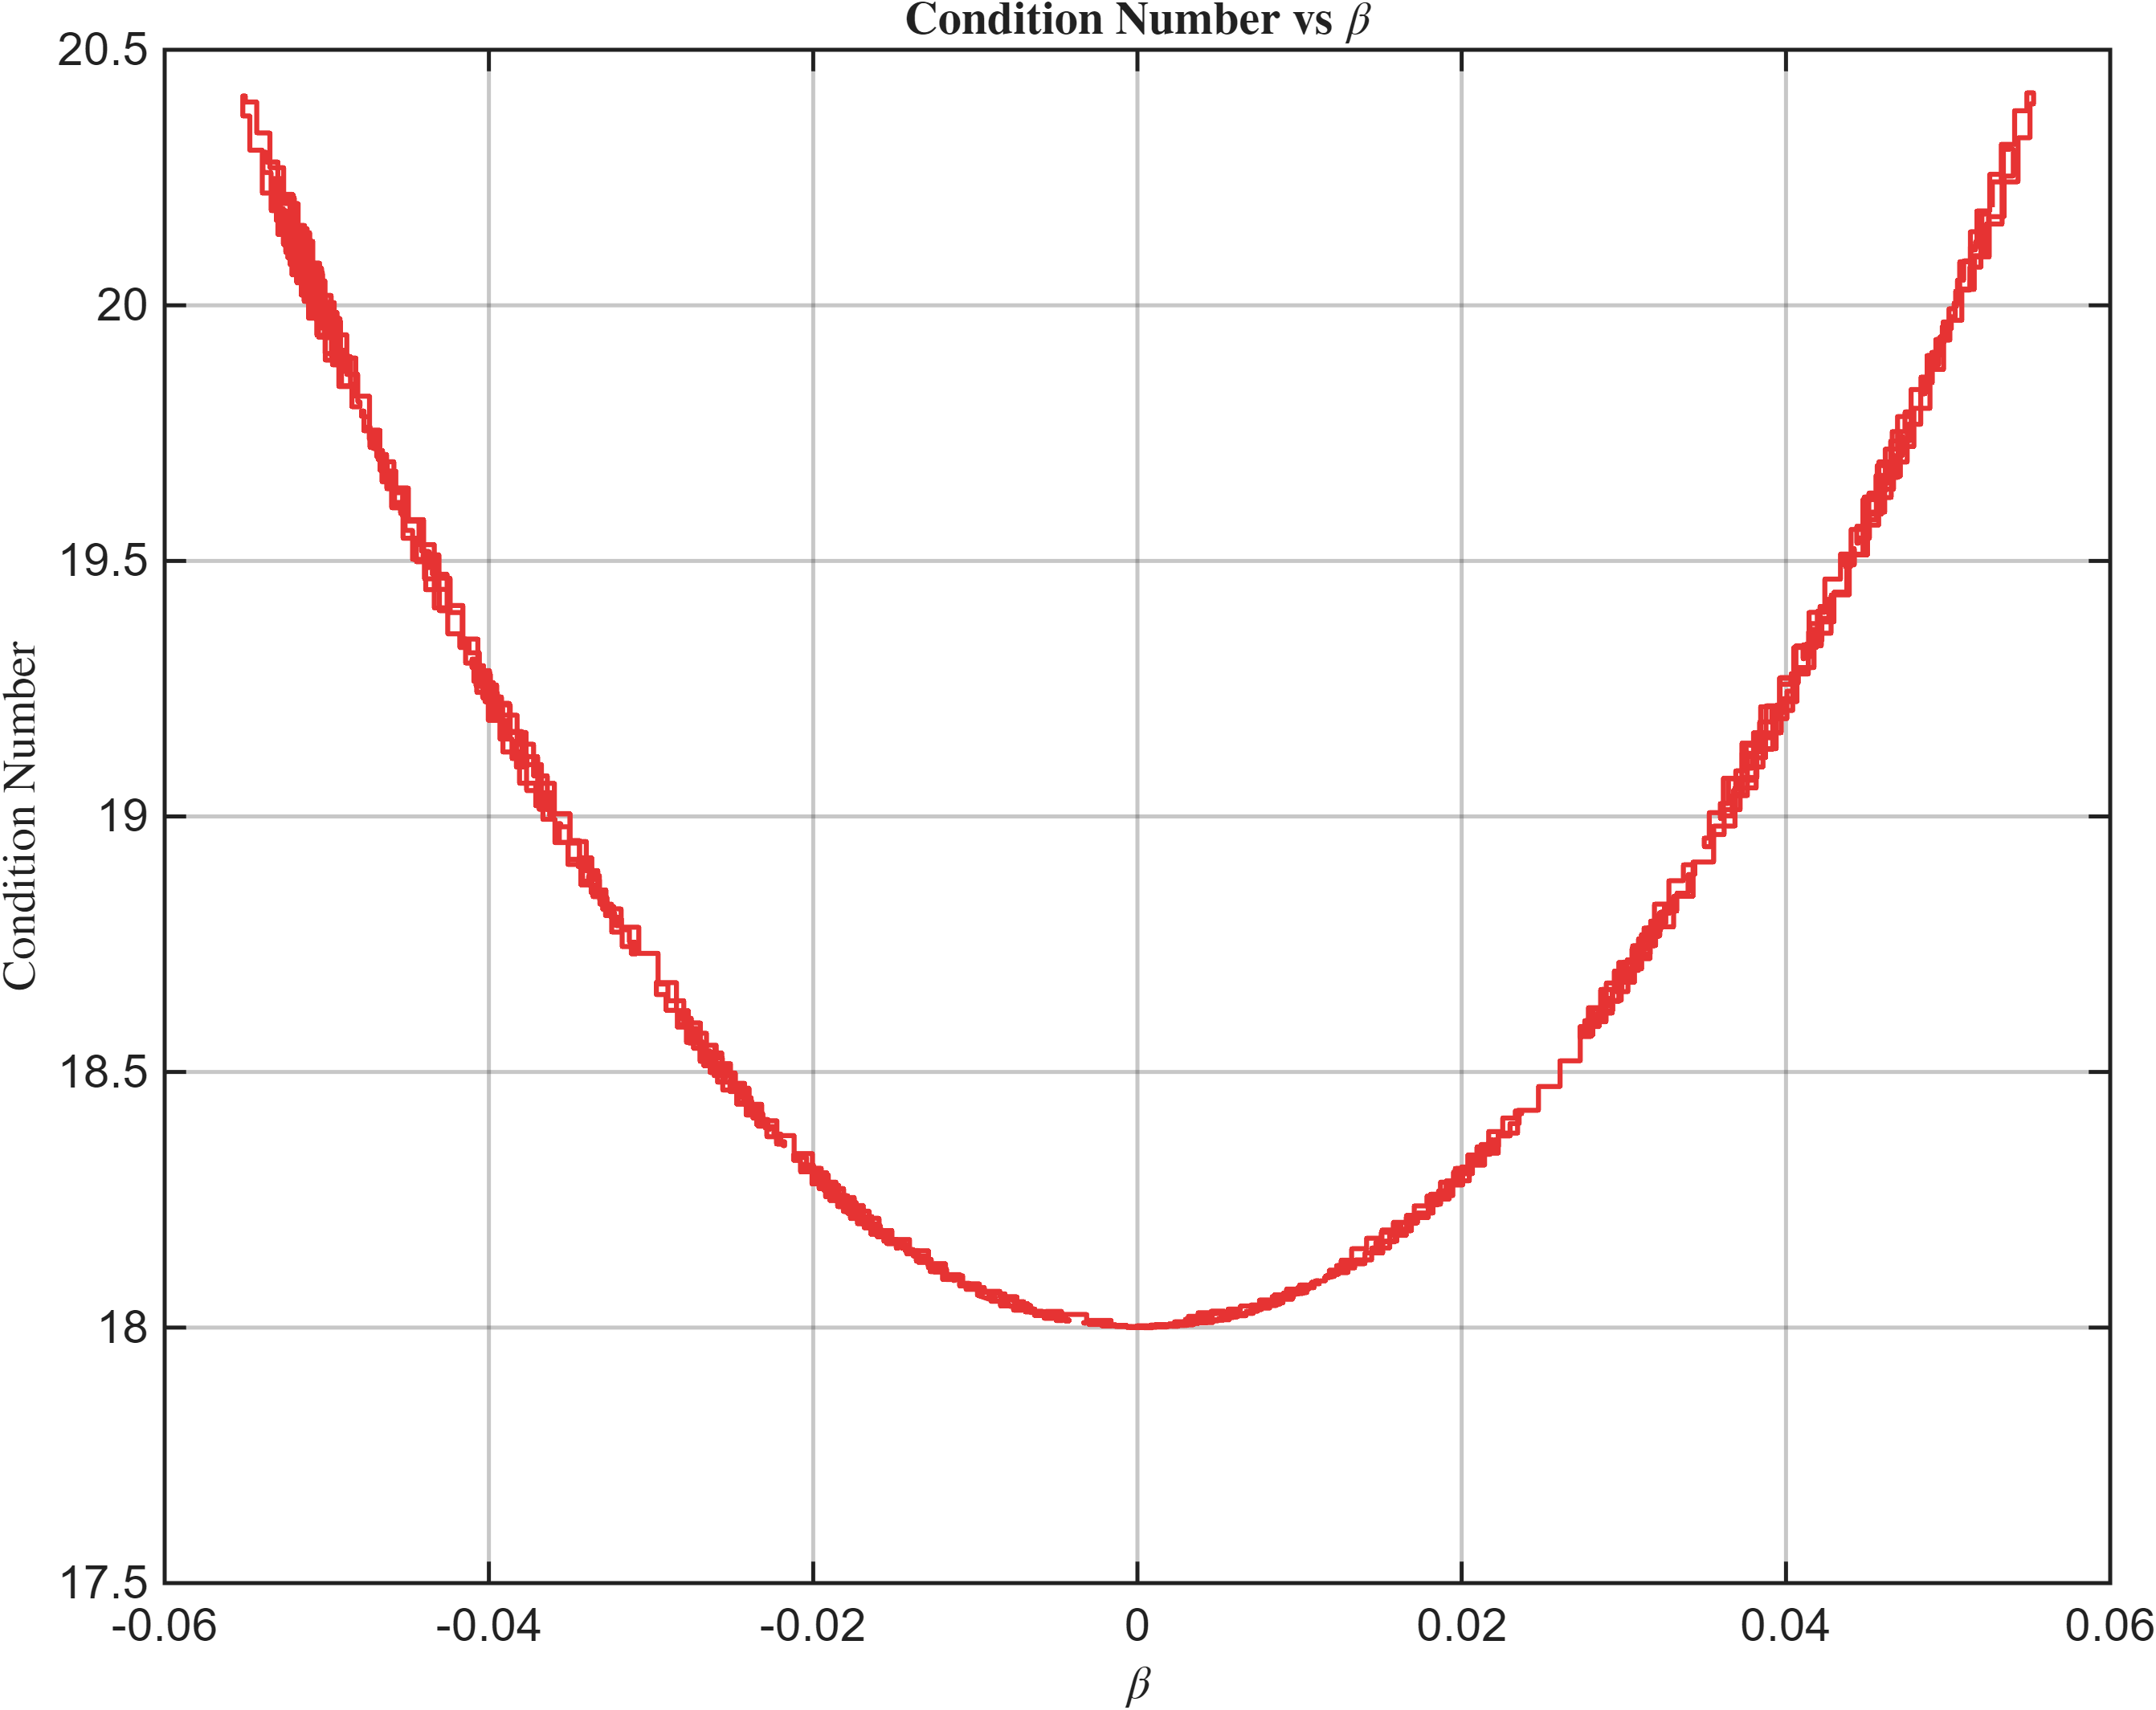
\includegraphics[width=0.48\textwidth]{img/condition_sweep/Pose_condition_beta/condition_vs_pose_beta}}
	\caption{تغییرات عدد شرط $\kappa$ در محورهای زاویه‌ای $\alpha$ و $\beta$}
	\label{fig:results-cond-alpha-beta}
\end{figure}

مشاهده می‌شود که با افزایش زاویه‌ی انحراف از حالت افقی، عدد شرط به صورت یکنواخت افزایش می‌یابد. با این حال، دامنه‌ی این افزایش بسیار محدود است: $\kappa$ از کمینه‌ی $18$ در حالت تراز، حداکثر به $20$ در زاویه‌ی $3$ درجه می‌رسد. این مقادیر همچنان در محدوده‌ی کاملاً ایمن قرار دارند و نشان می‌دهند که سیستم برای زوایای کوچک رول و پیچ (که در کاربری‌های عملی مورد نیاز است) از پایداری سینماتیکی کافی برخوردار است.

\subsection{جمع‌بندی تحلیل تکینگی}
\label{subsec:results-sing-summary}

نتایج عددی ارائه‌شده، تصویر روشنی از سلامت سینماتیکی فضای کاری ارائه می‌دهند. مهم‌ترین یافته آن است که \textbf{تنظیم $\gamma$ در حدود $\pi/4$} شرط اساسی برای قرار گرفتن در ناحیه‌ی ایمن و به‌دور از تکینگی است. با رعایت این شرط، سیستم قادر است کل صفحه‌ی افقی را با عدد شرط کمتر از $35$ بپیماید و زوایای رول و پیچ تا $0.06$ رادیان ($\approx 3.4^\circ$) را بدون خطر بدحال شدن ماتریس $\Gamma$ تحمل کند. این نتایج، مبنای عملی برای طراحی مسیرهای حرکتی ایمن و اجتناب از پیکربندی‌های ناپایدار فراهم می‌آورند و مکمّل تحلیل تحلیلی ارائه‌شده در بخش \ref{sec:method-singularity} هستند.

%----------------------------------------------------
\subsubsection{تحلیل جریان‌های تخصیص‌یافته به سیم‌پیچ‌ها}
\label{subsubsec:results-currents}

جریان‌های عبوری از ۱۶ سیم‌پیچ، که در شکل‌های \ref{fig:results-currents-xy} تا \ref{fig:results-currents-gamma} برای کلیه‌ی آزمون‌های گام رسم شده‌اند، حاصل یک نگاشت جبری بلافصل از پیچش مطلوب از طریق وارون شبه‌مور-پنروز ماتریس $\Gamma$ هستند، نه کمّیتی که مستقیماً از یک فرآیند فیزیکی اندازه‌گیری شده باشد. با این حال، از آن‌جا که این جریان‌ها حلقه‌ی واسط میان کنترل‌کننده و شبیه‌ساز فیزیکی را تشکیل می‌دهند، بازبینی کیفی آن‌ها برای تأیید صحت عملکرد زنجیره‌ی تخصیص ضروری است.

نخستین مشاهده‌ی قابل‌توجه آن است که شکل کلی جریان‌ها در هر یک از درجات آزادی، به‌طور مشهودی از نیمرخ پاسخ پله‌ی همان محور پیروی می‌کند. به‌عنوان مثال، جهش اولیه‌ی جریان‌ها که برای تأمین نیروی حداکثری (نظیر $F_x \approx 30~\text{N}$) ضروری است، دقیقاً با فاز «جهش جبرانی» در منطق فازی هم‌زمان است و فروافتادگی متعاقب نیز به همان صورت در دامنه‌ی جریان‌ها بازتاب می‌یابد. این تطابق شکلی، ریشه در ماهیت معادلات سینماتیک وارون دارد که بردار پیچش را به‌طور خطی و آنی به جریان‌ها نگاشت می‌دهد؛ بنابراین، هر مشخصه‌ی دینامیکیِ حاضر در فرمان کنترلی، بلافاصله در فضای جریان نیز رونوشت می‌شود. علاوه بر این، وابستگی ماتریس $\Gamma$ به موقعیت و جهت‌گیری لحظه‌ای جسم متحرک ($\mathbf{x}$) سبب می‌شود که تغییرات پیکربندی نیز بر دامنه و فاز نسبی جریان‌ها اثر بگذارند و الگوی نهایی را اندکی از یک مقیاس‌بندی ساده‌ی فرمان دور سازند.

در نگاه اول، نوسانات نسبتاً تند و پرشیبی که در برخی از کانال‌ها دیده می‌شود ممکن است شائبه‌ی ناپایداری را ایجاد کند. اما با در نظر گرفتن مقیاس محور زمان و دامنه‌ی تغییرات، روشن می‌شود که این نوسانات در محدوده‌ای رخ می‌دهند که محدودکننده‌ی نرخ $80~\text{A/s}$ و بلوک اشباع $[-9,9]~\text{A}$ آن را مجاز شمرده‌اند. به بیان دیگر، سیستم هرگز فرمانی فراتر از توان سخت‌افزاری خود دریافت نکرده و این نوسانات، صرفاً پاسخ دینامیکی کنترل‌کننده‌ی فازی را که در فضای نیرو و گشتاور تحلیل شد، به فضای جریان منتقل کرده‌اند. بنابراین، رفتار مشاهده‌شده از منظر امکان‌پذیری عملیاتی، کاملاً موجه و تحت کنترل بوده است.

الگوی هم‌کاری میان سیم‌پیچ‌ها نیز با آنچه از ساختار معادلات $\Gamma^\dagger$ انتظار می‌رود سازگار است. جفت‌هایی از سیم‌پیچ‌ها که نسبت به مرکز آرایه موقعیتی متقارن دارند، جریان‌هایی دقیقاً با علامت مخالف اما با شکل یکسان حمل می‌کنند؛ به‌گونه‌ای که گویی یک نسخه‌ی منفی از دیگری است. برخی دیگر، یک شکل موج مشابه را با ضرایب مقیاس متفاوت بازتولید می‌کنند. این رفتار جمعی و هم‌بسته، بازتاب مستقیم نحوه‌ی ترکیب میدان‌های مغناطیسی برای تولید برآیند پیچش خالص است و کاملاً از استنتاج ریاضی $\Gamma$ برمی‌آید. با این وجود، ارائه‌ی یک تحلیل جامع از ساختار فضایی جریان‌ها و قواعد حاکم بر آن نیازمند گردآوری و بررسی مجموعه‌ای بسیار گسترده‌تر از داده‌ها (شامل مانورهای ترکیبی و مسیرهای متغیر) است و بهتر است به فاز اعتبارسنجی تجربی یا یک مطالعه‌ی عددی مستقل واگذار شود.

آنچه در چارچوب این شبیه‌سازی اهمیت دارد، اثبات آن است که زنجیره‌ی تخصیص کنترلی، با وجود ابعاد بالا و استفاده از وارون شبه‌مور-پنروز، تحت قیود سخت‌افزاری اشباع و نرخ محدود، جریان‌های پایدار، متقارن و عاری از تکینگی تولید کرده است. این نتایج، انتظار عملکرد ایمن و قابل پیش‌بینی را در هنگام انتقال به سخت‌افزار واقعی تقویت می‌کند.



\begin{figure}[htbp]
	\centering
	\subfloat[$X$]{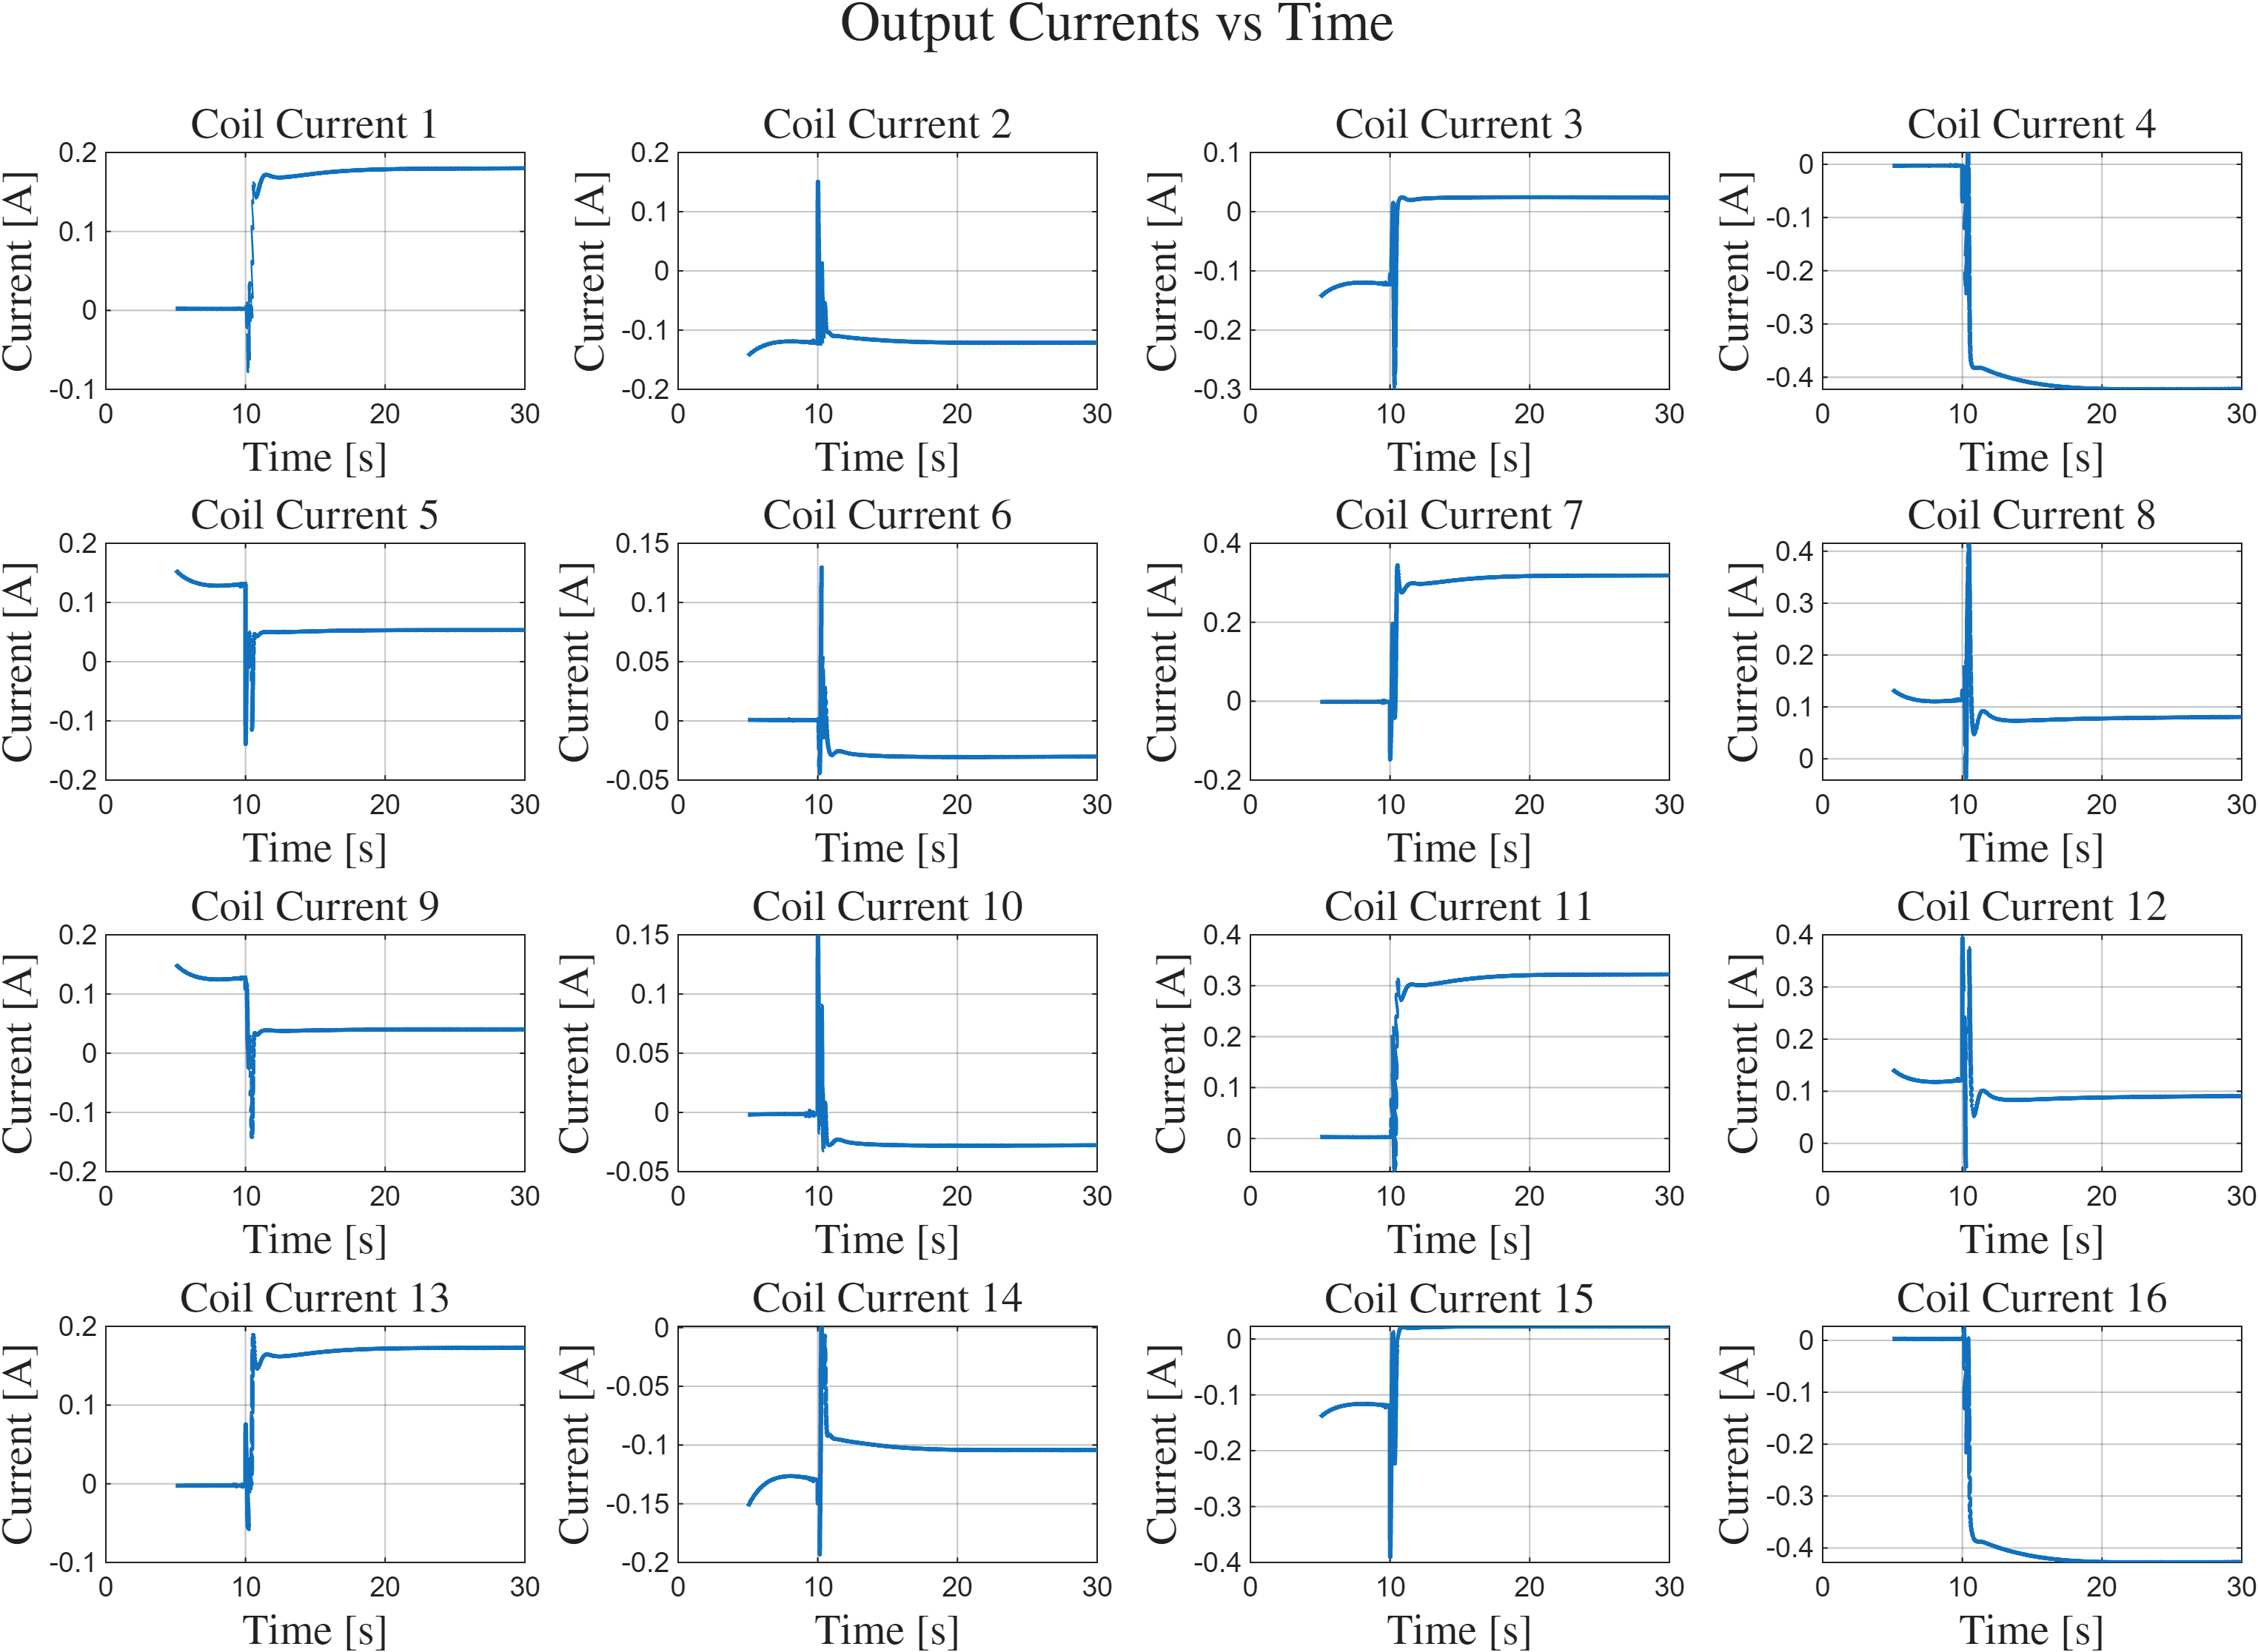
\includegraphics[width=0.48\textwidth]{img/step/x/output_currents}}
	\hfill
	\subfloat[$Y$]{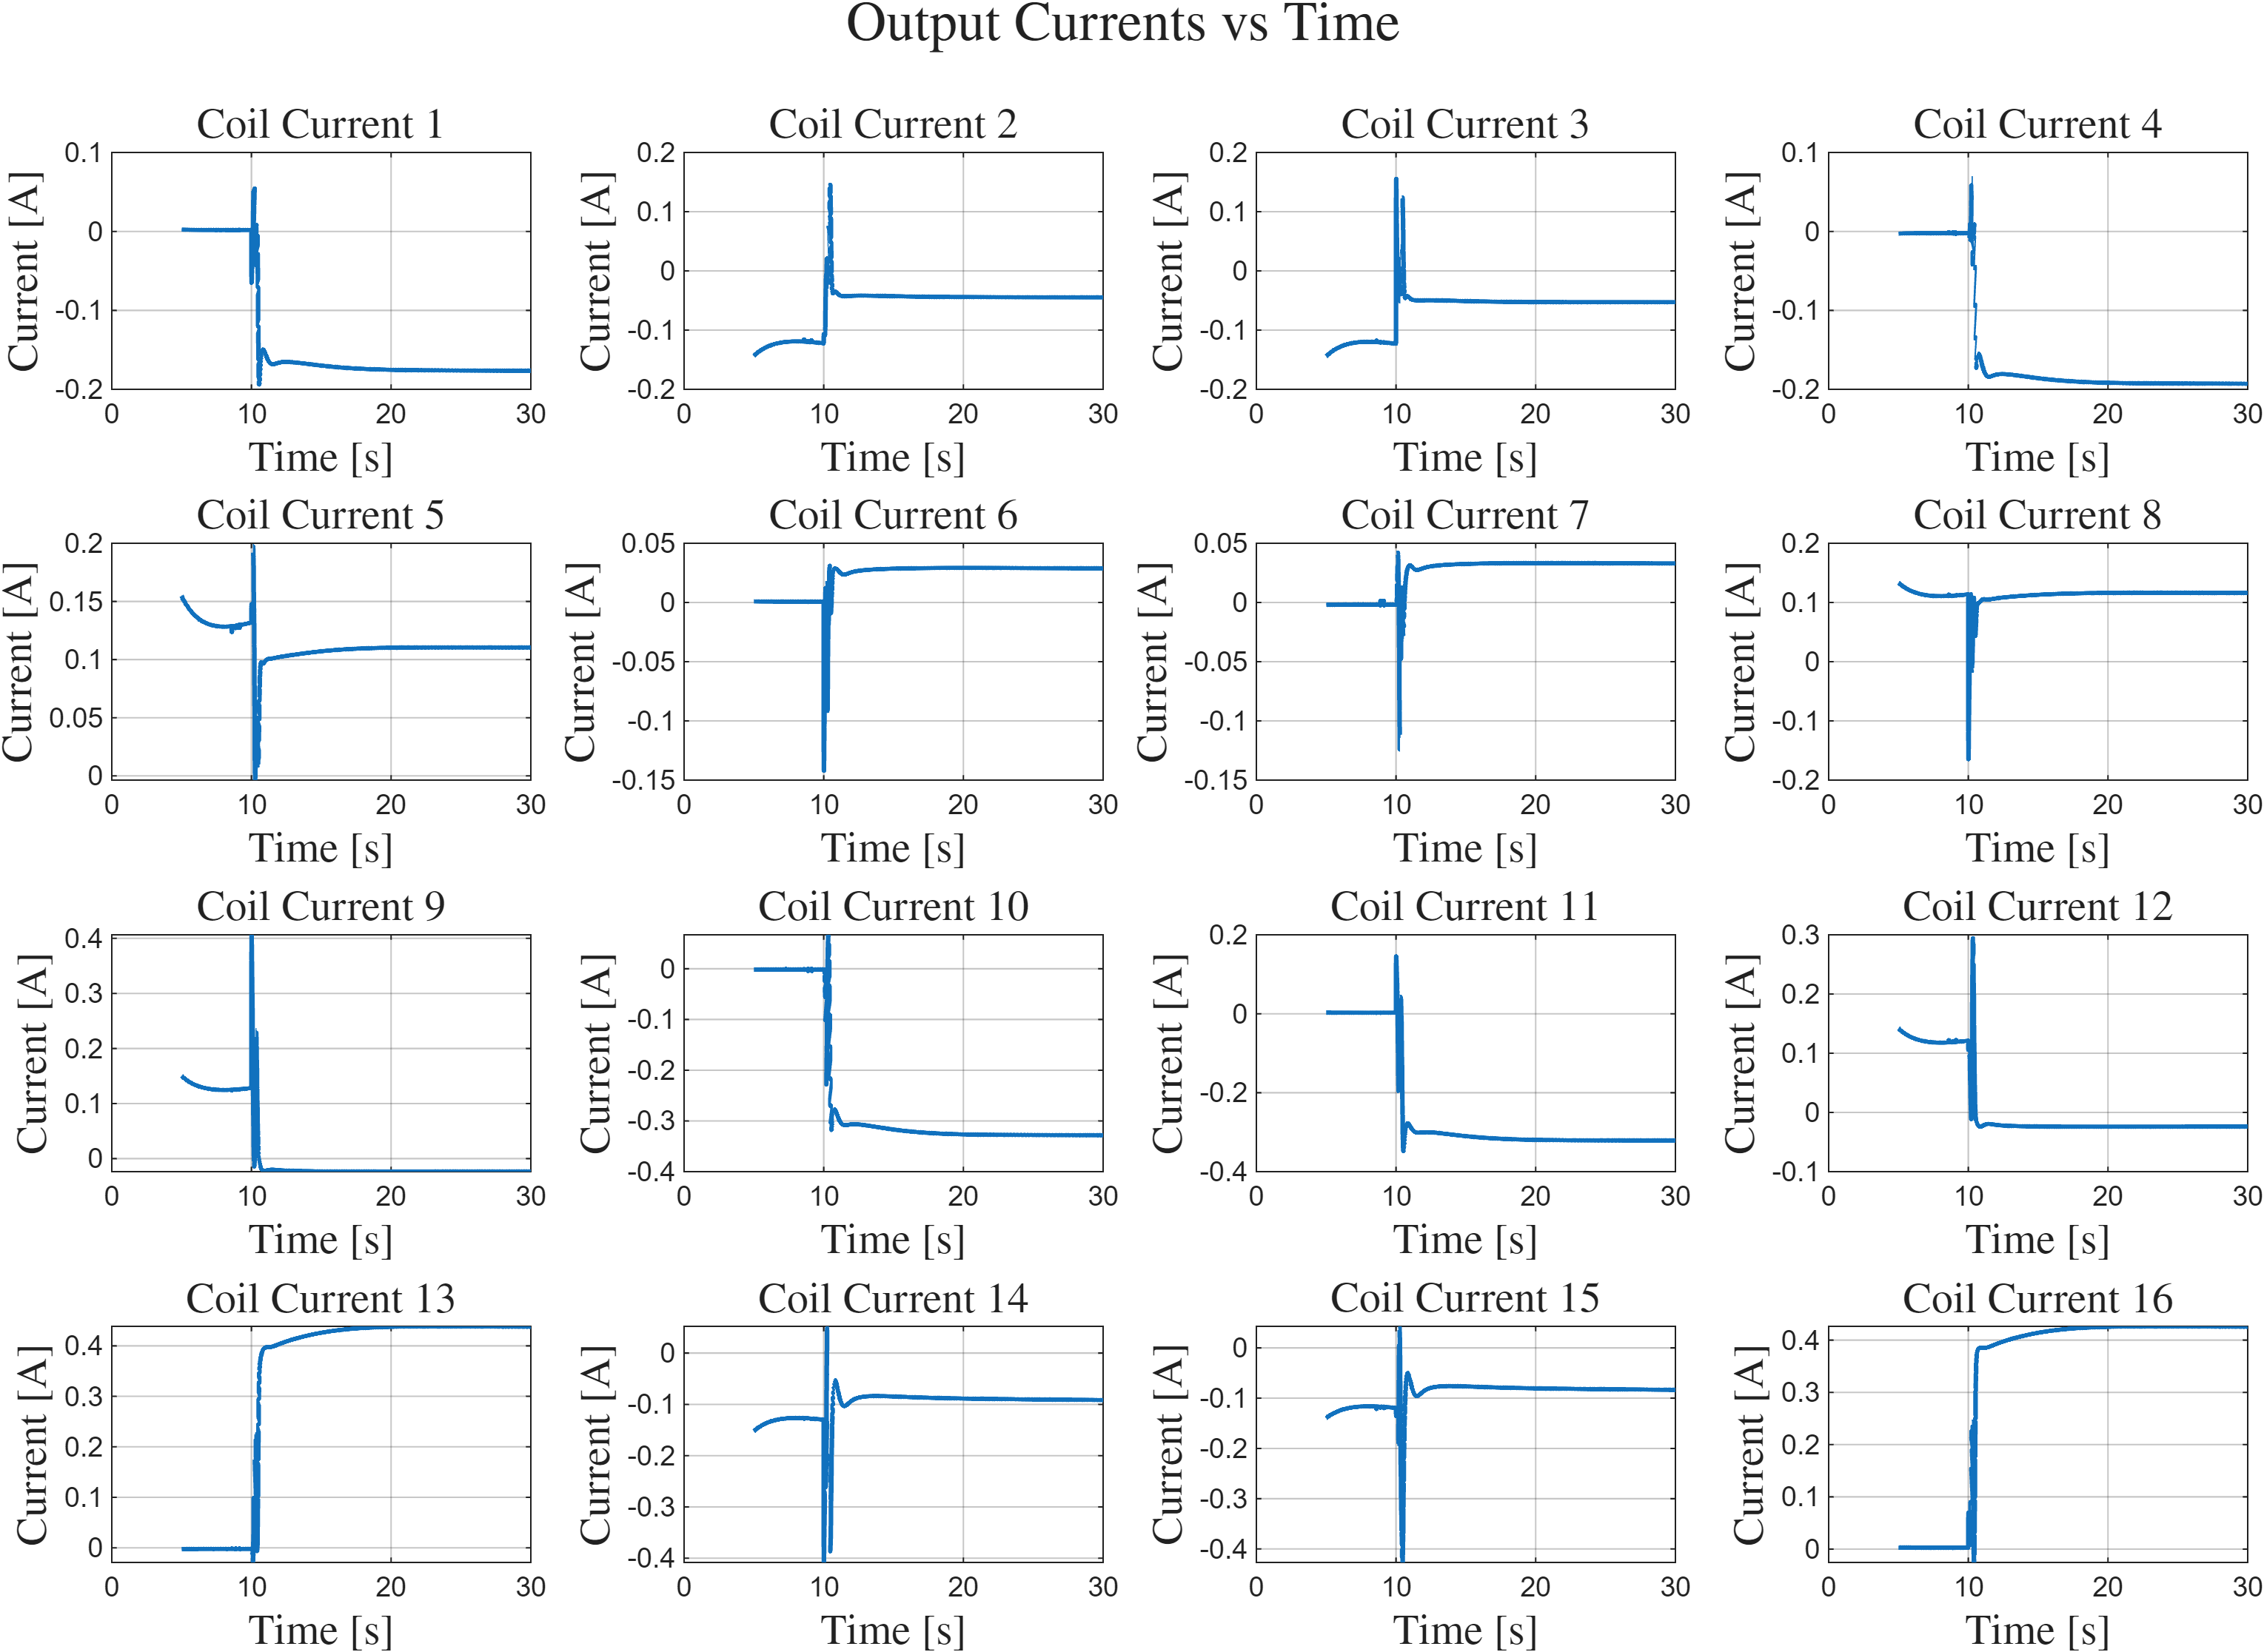
\includegraphics[width=0.48\textwidth]{img/step/y/output_currents}}
	
	\caption{جریان سیم‌پیچ‌ها در محورهای $X$ و $Y$}
	\label{fig:results-currents-xy}
\end{figure}

\begin{figure}[htbp]
	\centering
	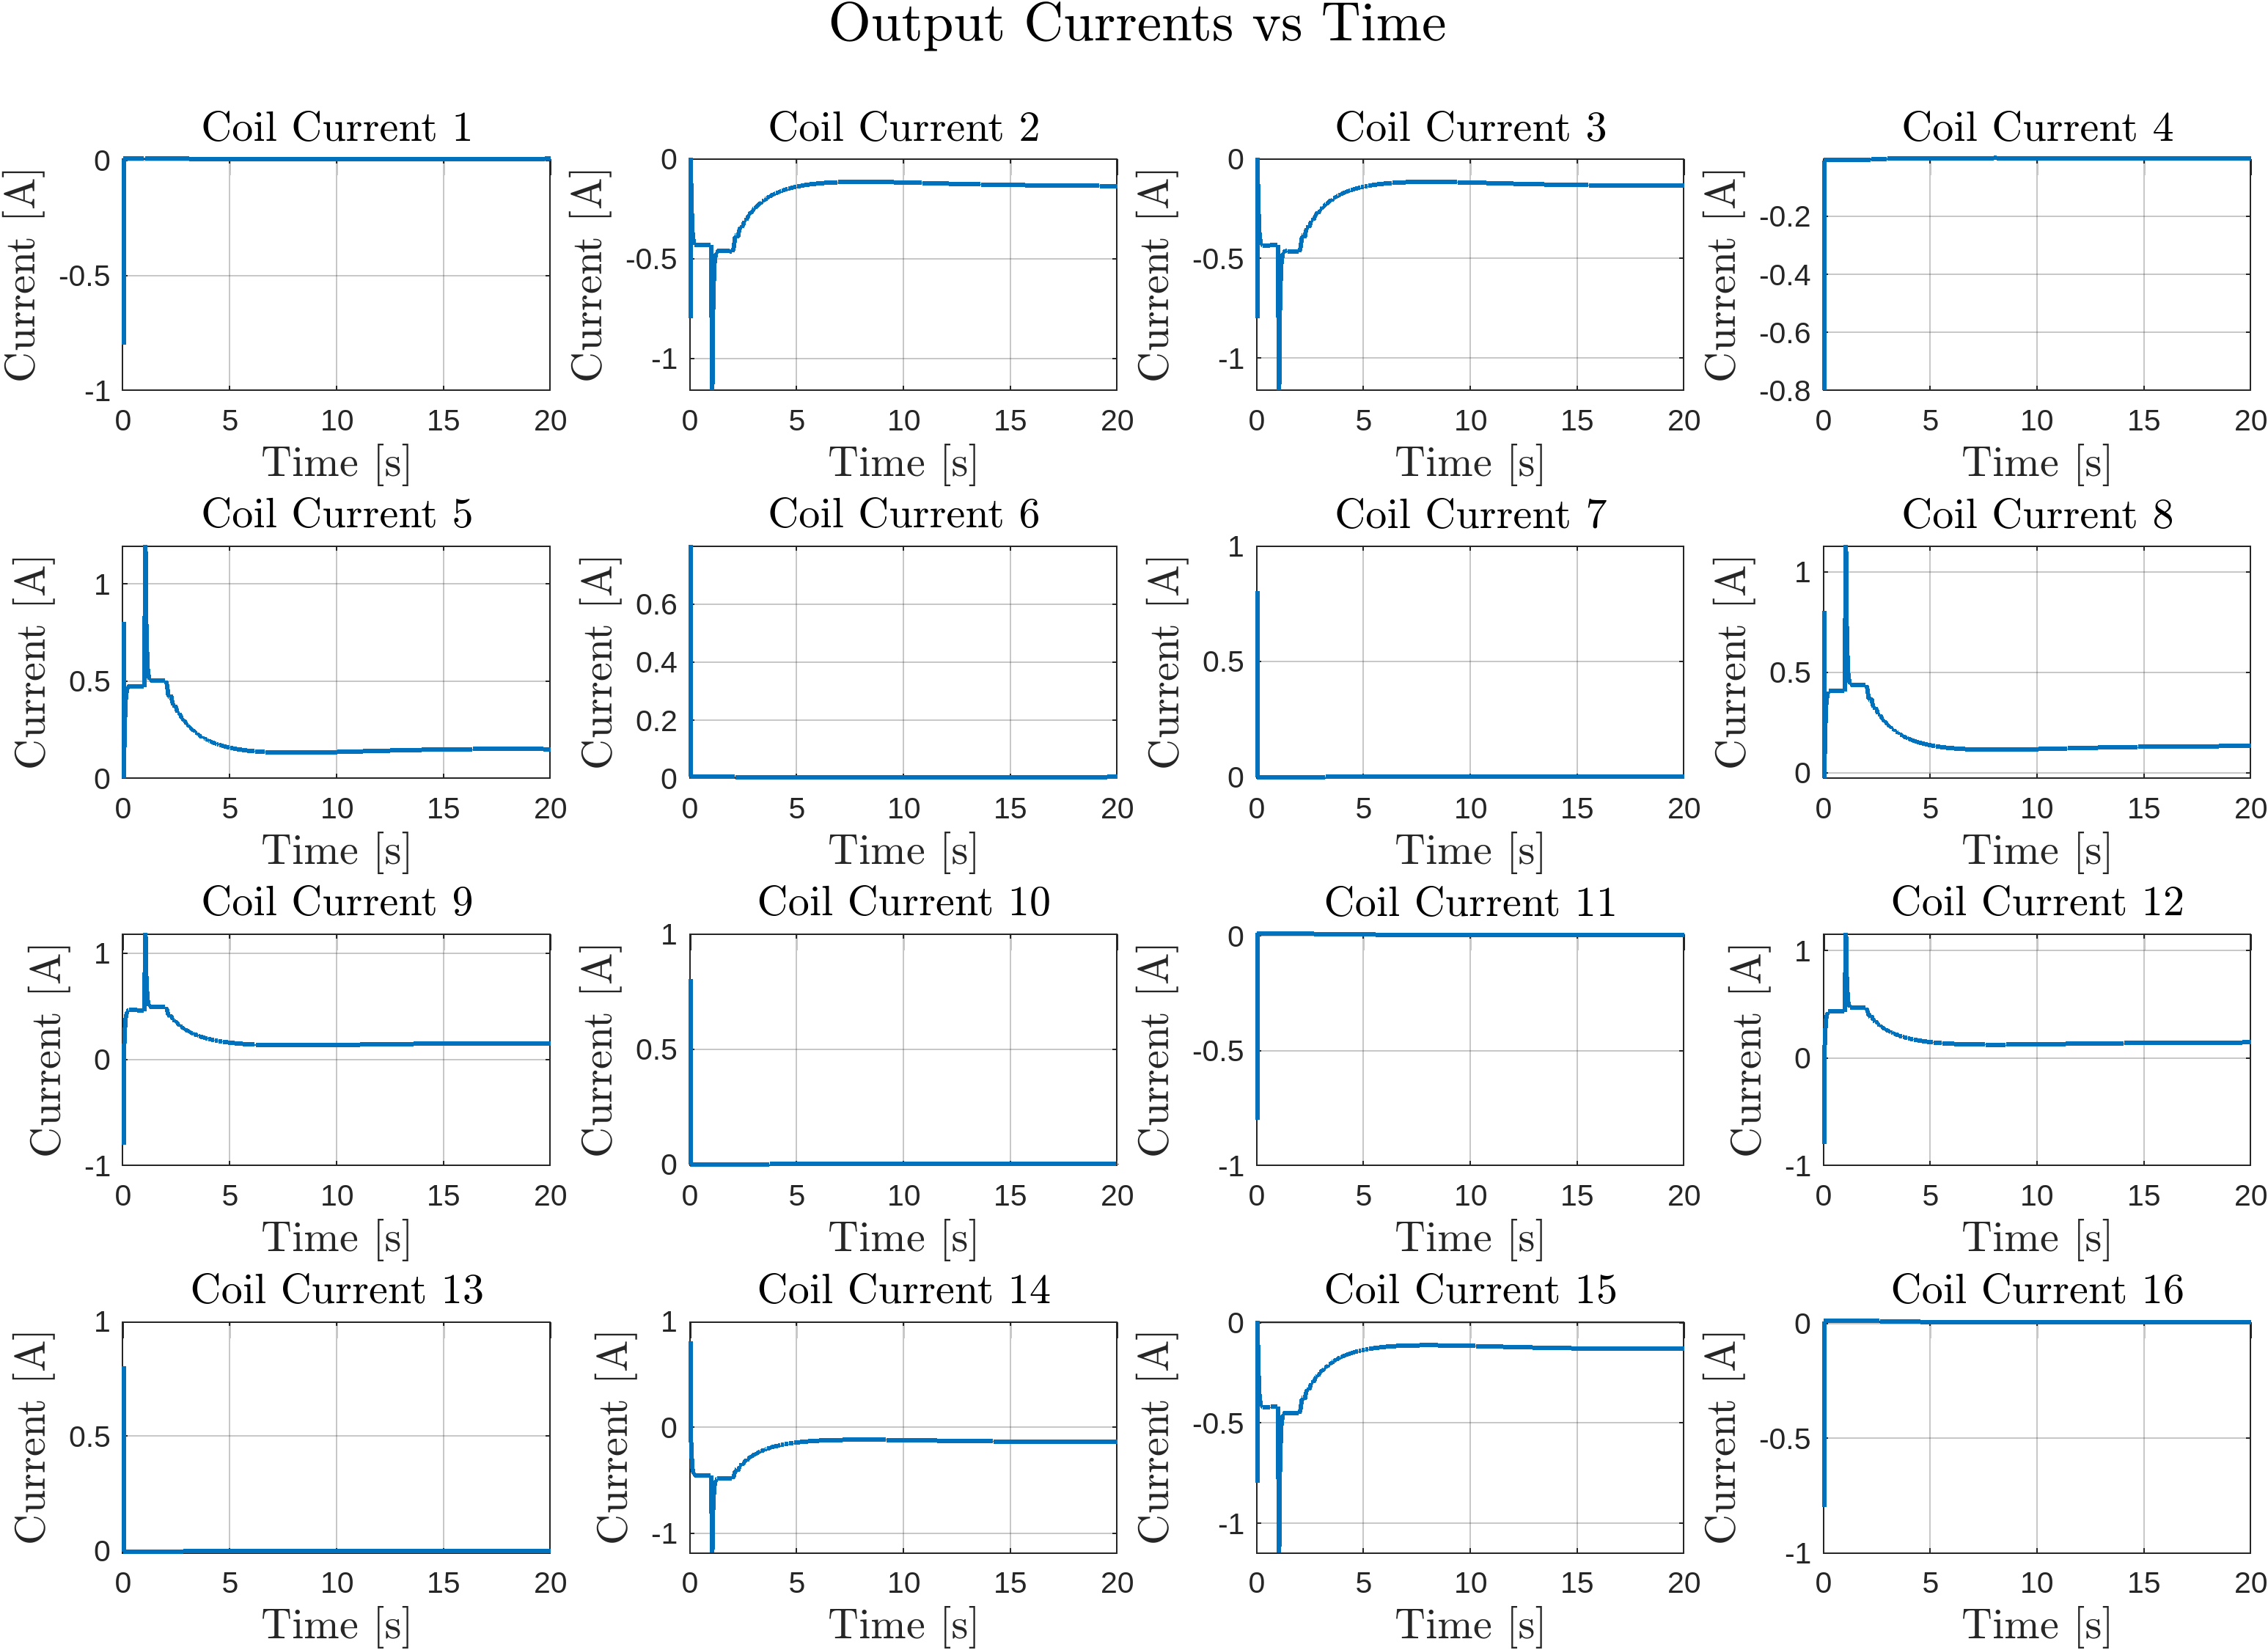
\includegraphics[width=0.75\textwidth]{img/step/z/output_currents}
	\caption{جریان سیم‌پیچ‌ها در محور $Z$}
	\label{fig:results-currents-z}
\end{figure}

%----------------------------------------------------

\begin{figure}[htbp]
	\centering
	\subfloat[$\alpha$]{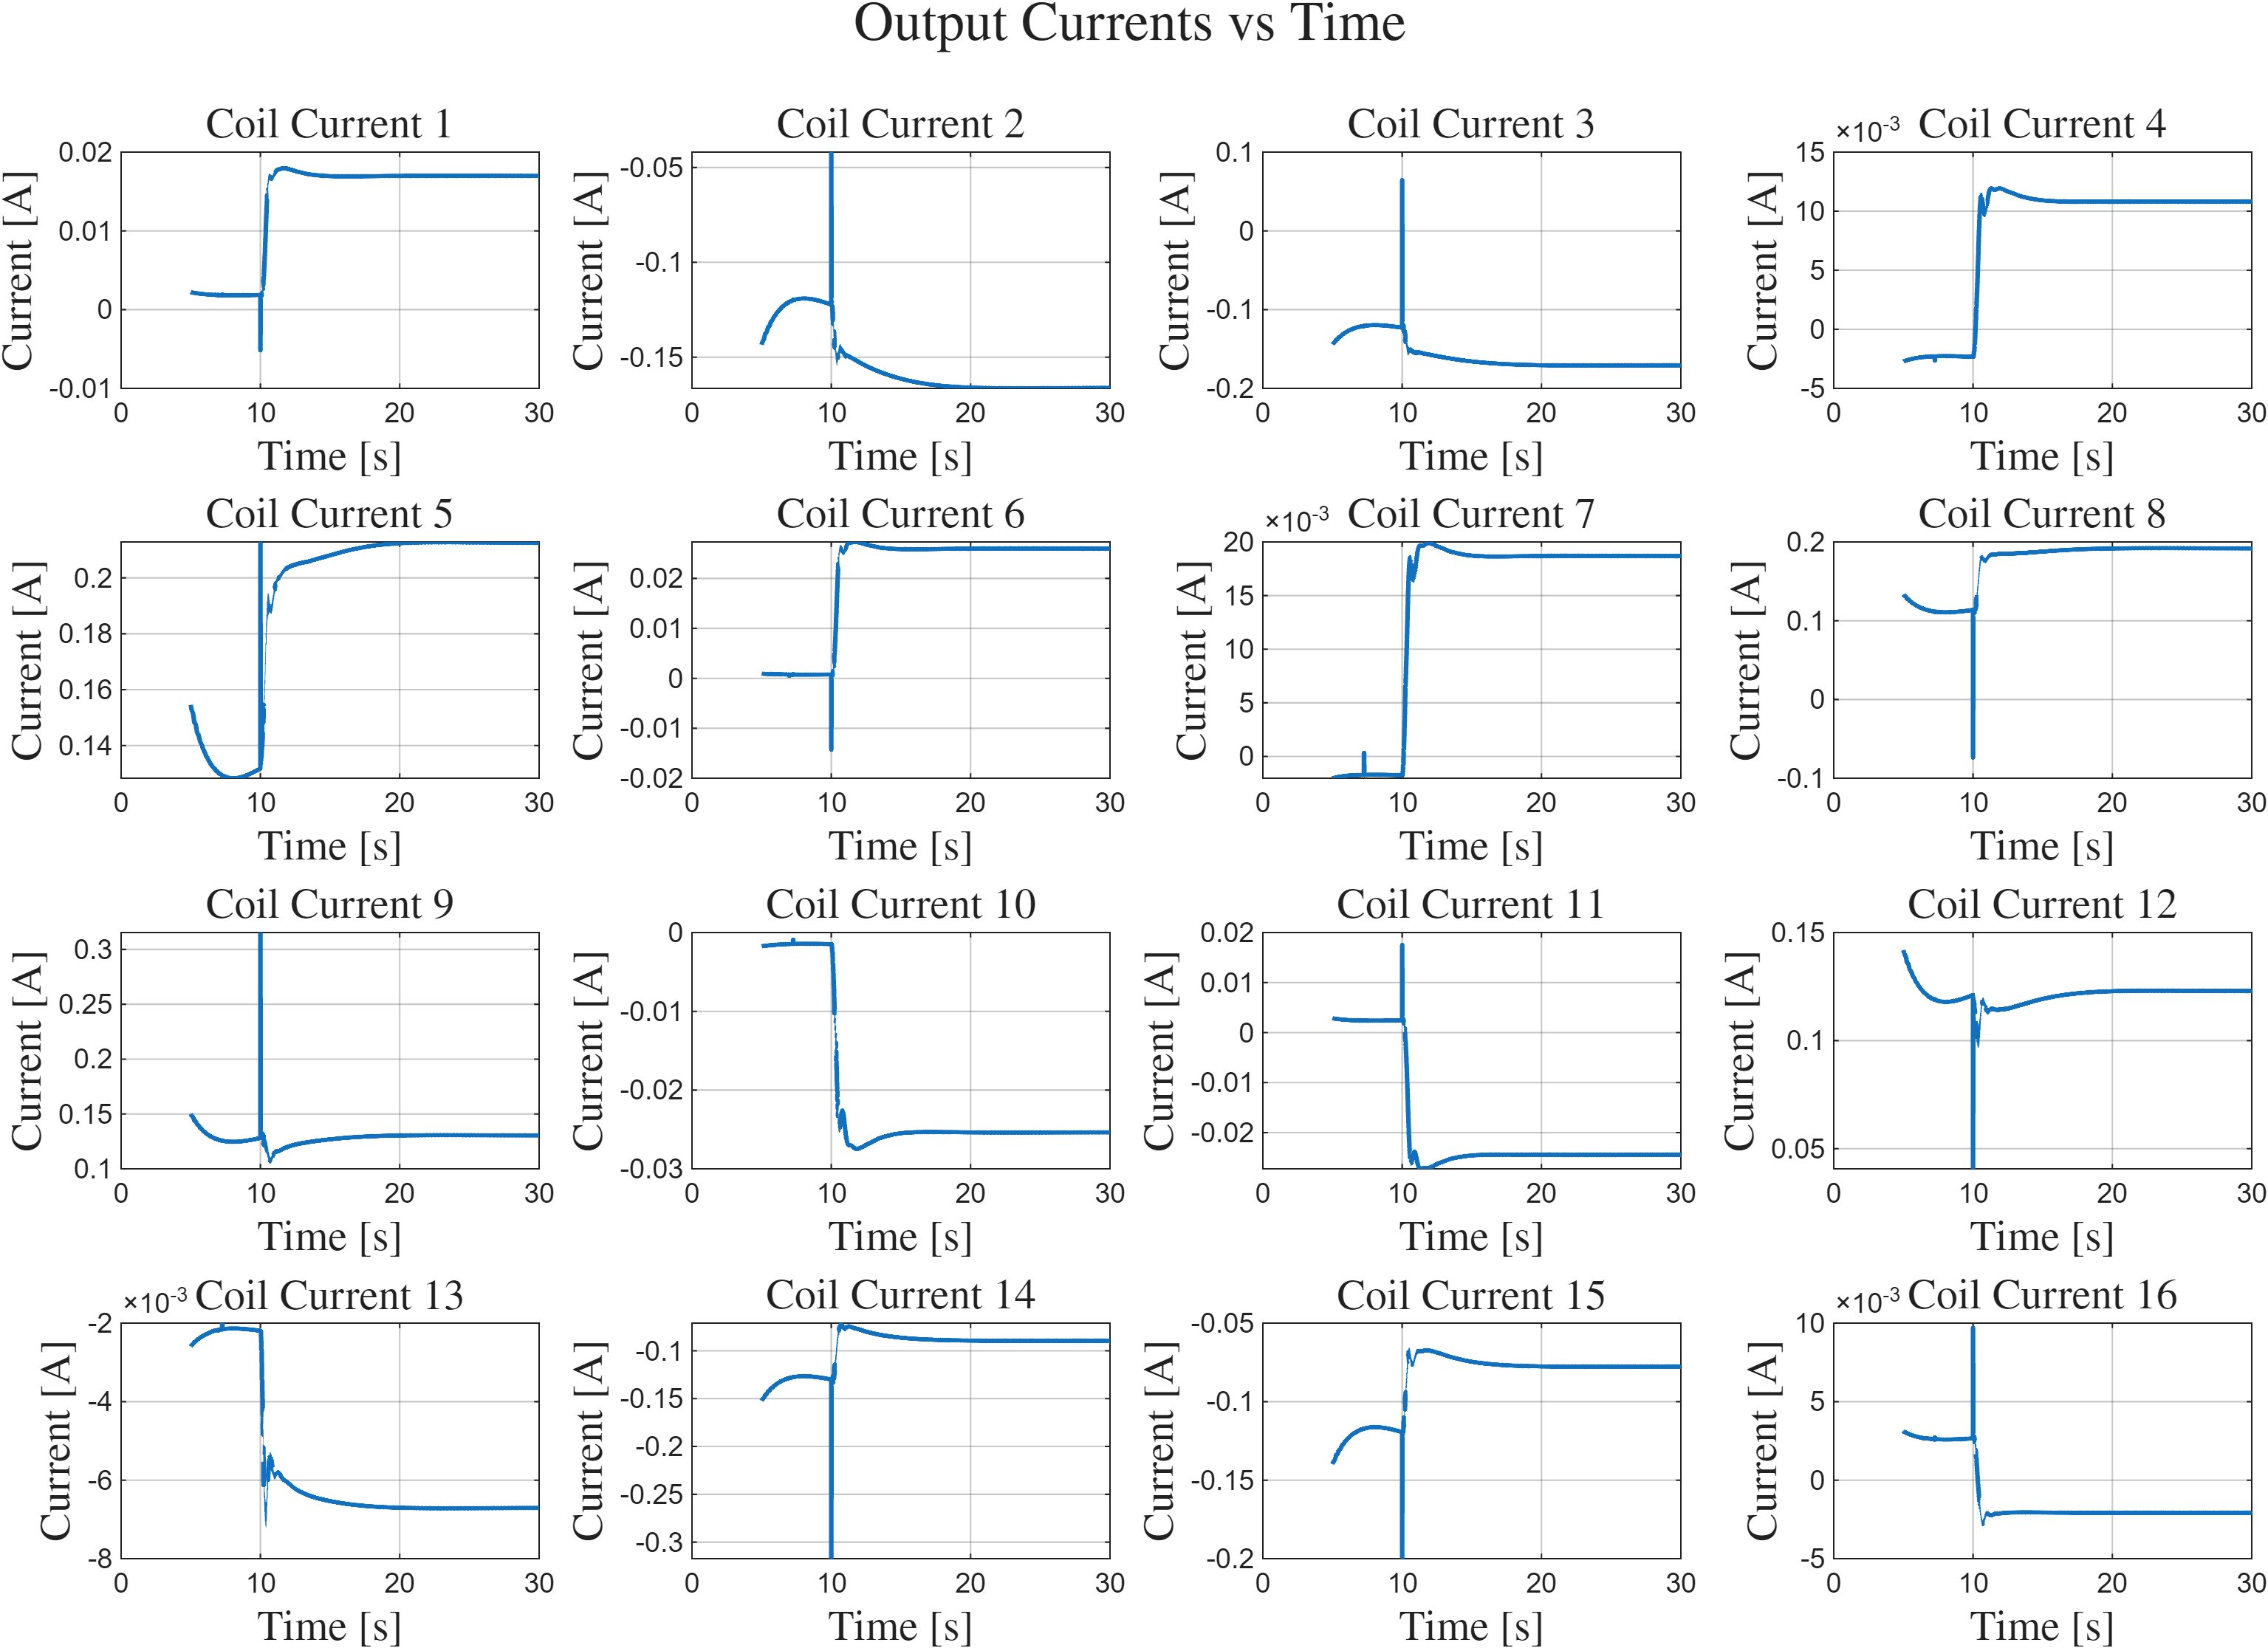
\includegraphics[width=0.48\textwidth]{img/step/alpha/output_currents}}
	\hfill
	\subfloat[$\beta$]{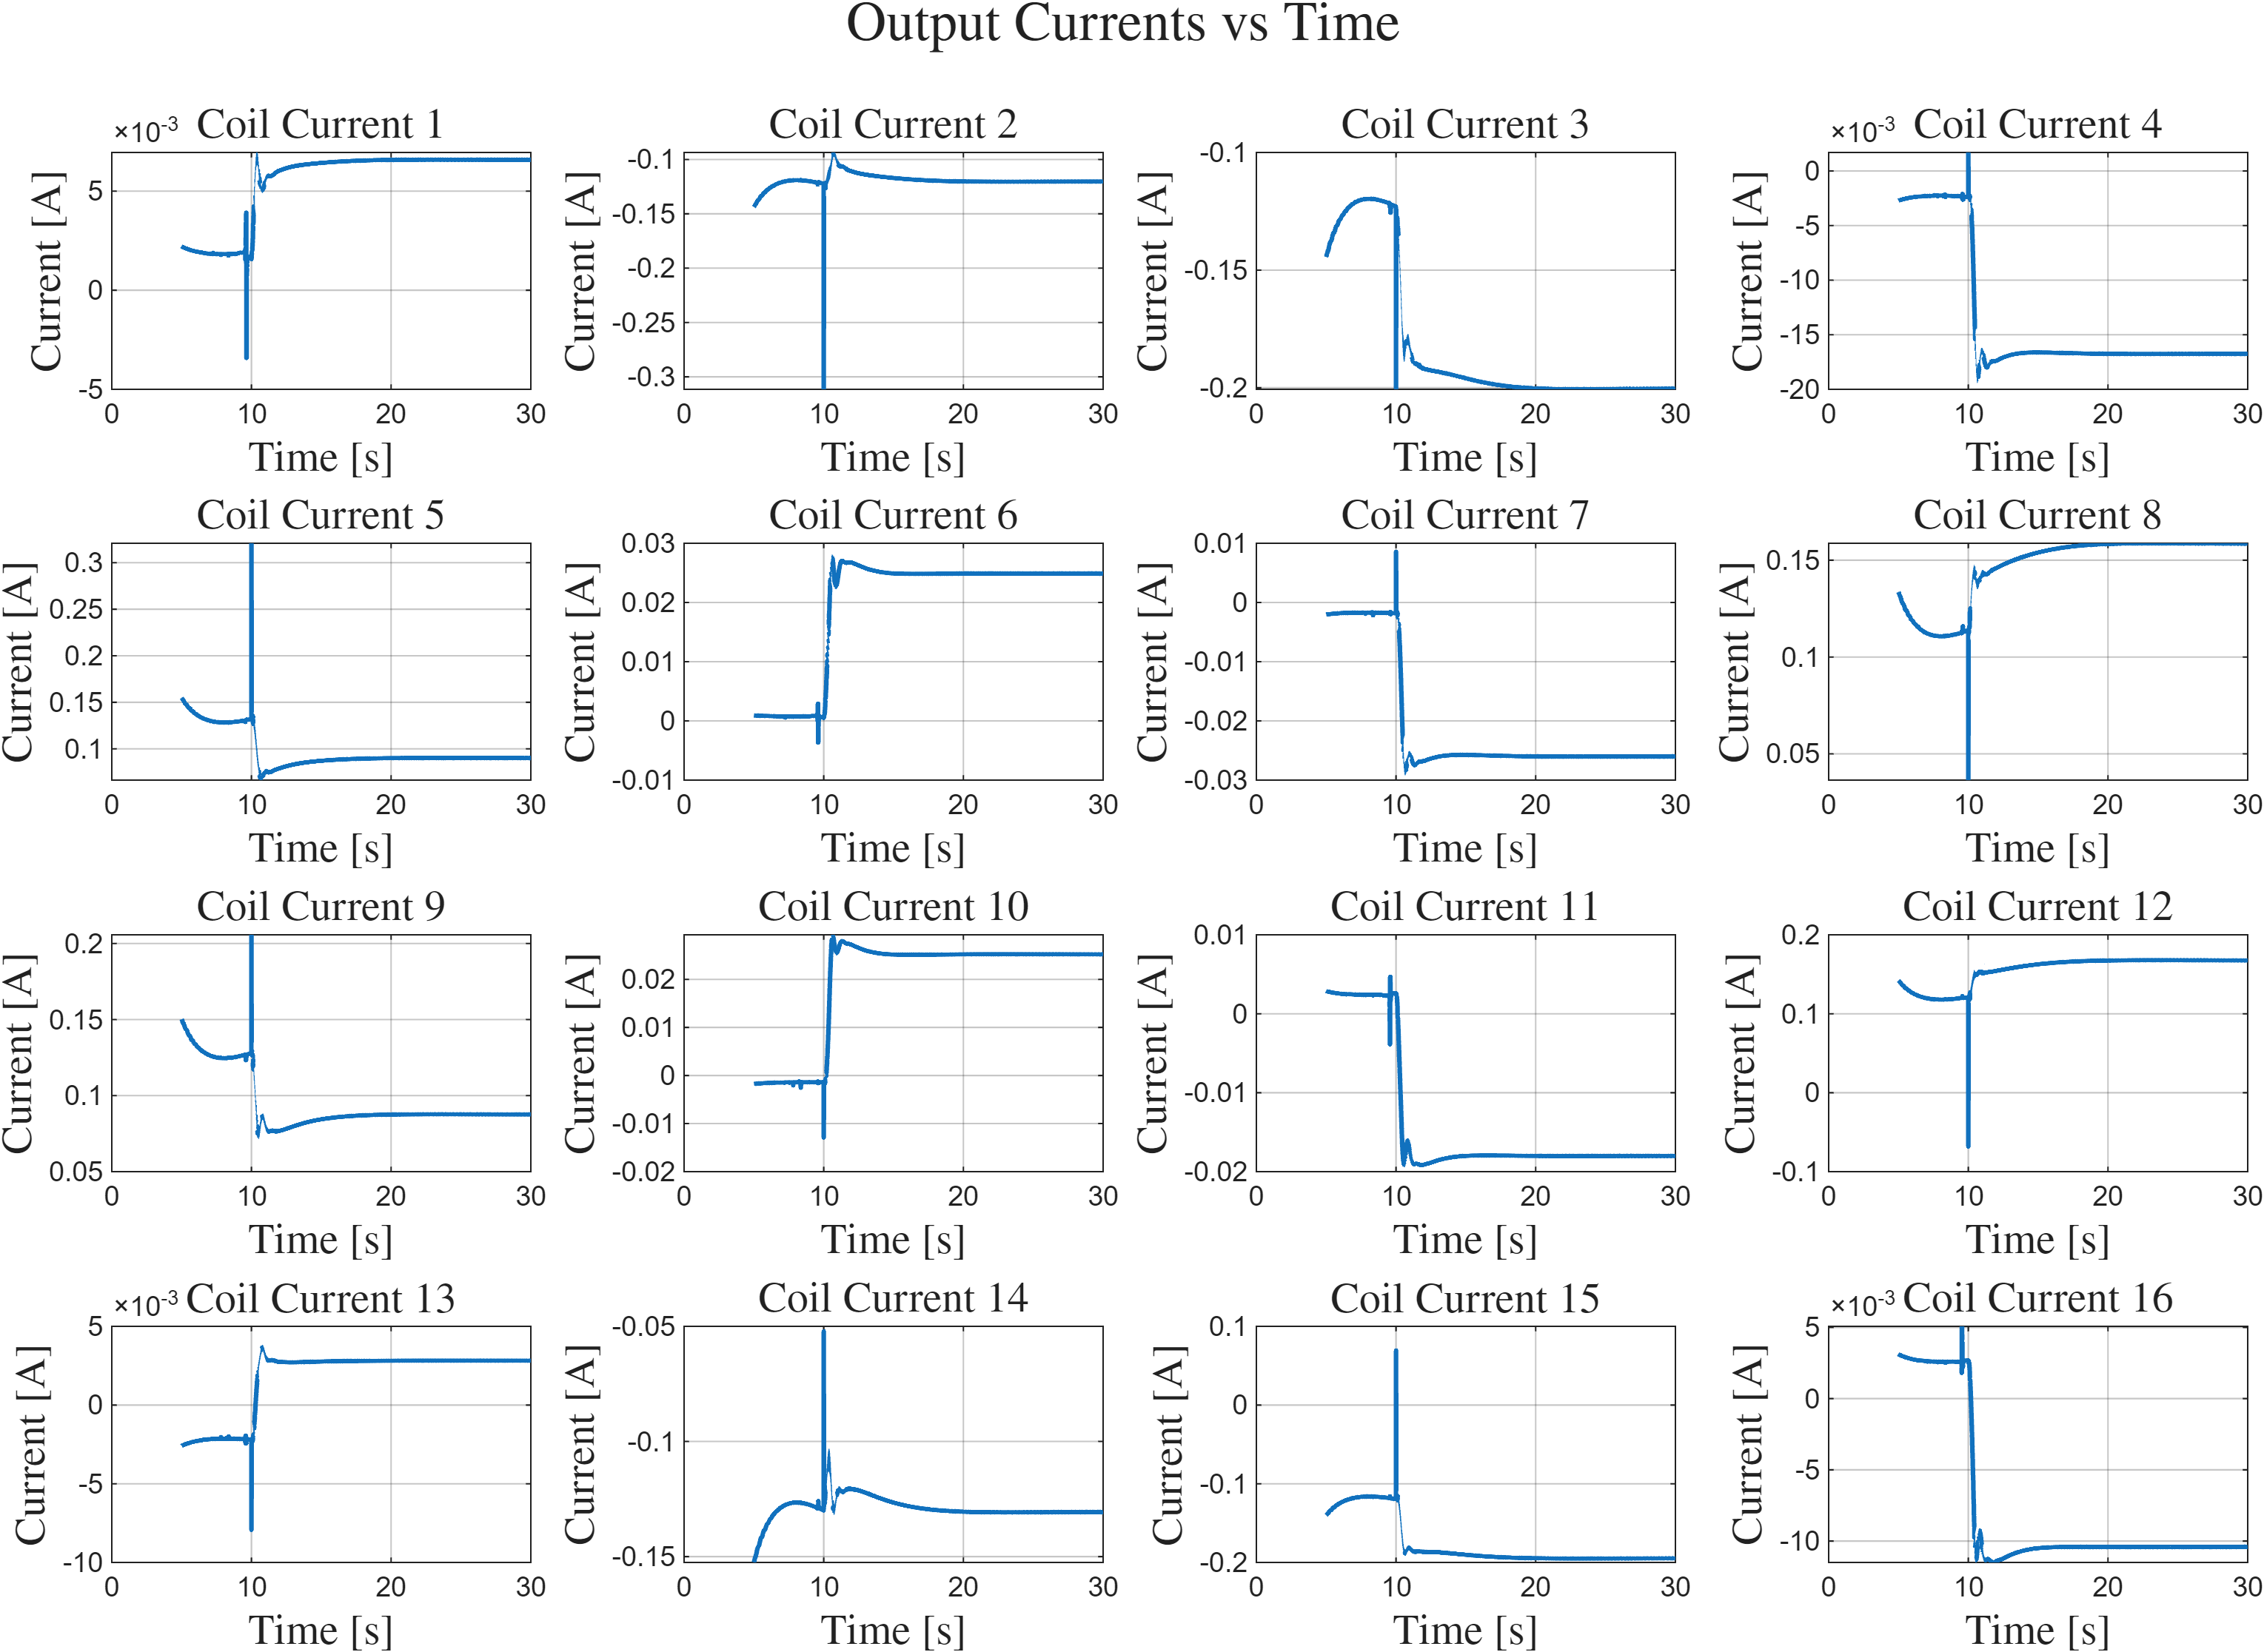
\includegraphics[width=0.48\textwidth]{img/step/beta/output_currents}}
	
	\caption{جریان سیم‌پیچ‌ها در محورهای $\alpha$ و $\beta$}
	\label{fig:results-currents-alpha-beta}
\end{figure}

\begin{figure}[htbp]
	\centering
	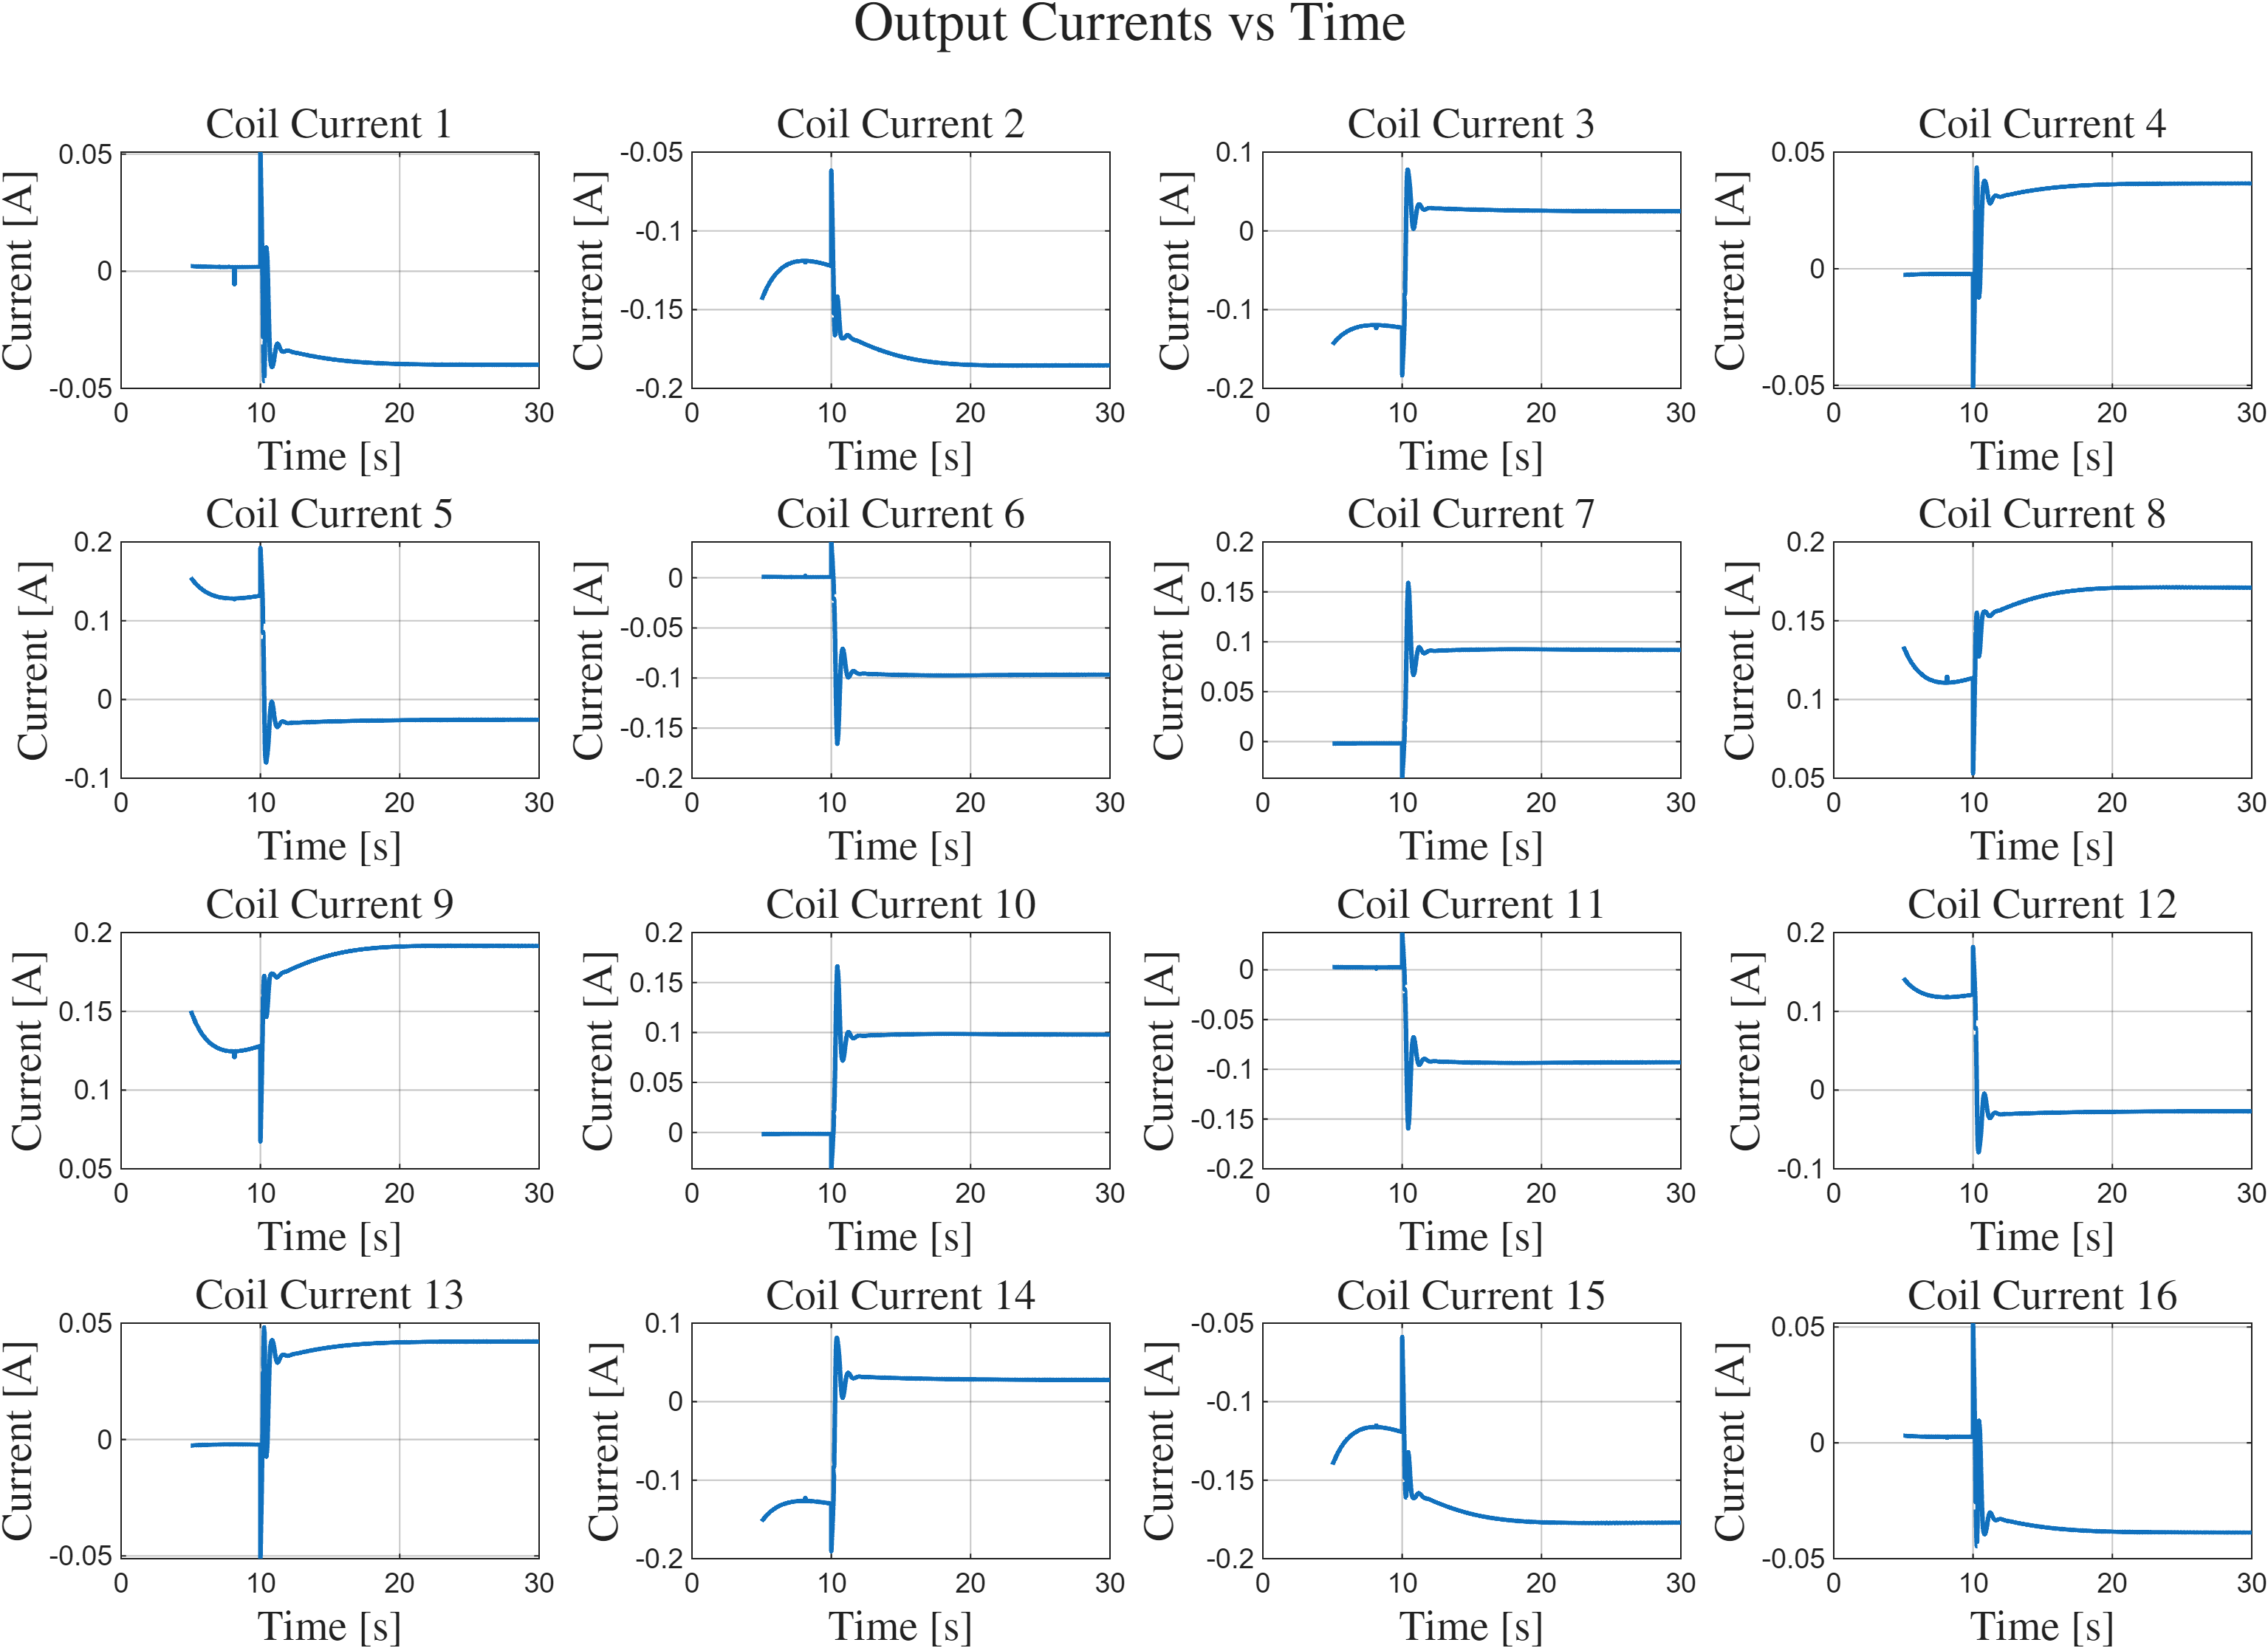
\includegraphics[width=0.75\textwidth]{img/step/gamma/output_currents}
	\caption{جریان سیم‌پیچ‌ها در محور $\gamma$}
	\label{fig:results-currents-gamma}
\end{figure}


\section{ارزیابی عملکرد در ردیابی مسیر منهتن}
\label{sec:results-manhattan}

آزمون نهایی برای موتور مغناطیسی شناور صفحه‌ای، تعقیب یک مسیر چندمرحله‌ای در صفحه‌ی $XY$ است که به‌طور هم‌زمان دقت ردیابی، سرعت پاسخ، و پایداری در برابر اغتشاشات متقاطع را محک می‌زند. بدین منظور، مسیر منهتن (\lr{Manhattan Trajectory}) که از توالی پله‌های متعامد تشکیل شده است، به‌عنوان یک سناریوی جامع طراحی و بر روی سیستم اعمال گردید. اهمیت این مسیر در آن است که برخلاف آزمون‌های پله‌ی مجزای پیشین، هر محور در حین حرکت محور دیگر باید موقعیت خود را ثابت نگه دارد و سپس با شتابی ناگهانی به نقطه‌ی بعدی جهش کند. چنین الگویی دقیقاً رفتار مورد انتظار از یک موتور صفحه‌ای واقعی در کاربری‌های جابه‌جایی دقیق را بازتاب می‌دهد و از این رو، موفقیت در آن به معنای تأیید نهایی چارچوب کنترلی پیشنهادی است.



\subsection{تعریف مسیر و منطق تولید}
\label{subsec:results-manhattan-def}

مسیر منهتن به‌کمک تابعی که منطق آن در ادامه تشریح می‌شود، به صورت برخط در محیط \lr{Simulink} تولید و به‌عنوان ورودی مرجع به کنترل‌کننده ارسال گردید. این تابع یک الگوی پلکانی با $N_{\text{steps}} = 5$ پله در هر راستا ایجاد می‌کند. طول کل حرکت در هر دو محور $L_x = L_y = 0.2$ متر در نظر گرفته شده است، در نتیجه هر پله دارای اندازه‌ی ثابت $\Delta x = \Delta y = 0.04$ متر می‌باشد.

زمان‌بندی مسیر به گونه‌ای است که بخش متحرک ابتدا یک گام در راستای $X$ برمی‌دارد و سپس یک گام در راستای $Y$، و این الگو تا پوشش کامل پنج پله تکرار می‌شود. بدین ترتیب، مسیر از $2N_{\text{steps}} = 10$ قطعه‌ی زمانی تشکیل می‌شود که مدت هر یک برابر با $t_{\text{seg}} = T_{\text{total}} / (2N_{\text{steps}})$ است و $T_{\text{total}}$ زمان کل در نظر گرفته شده برای حرکت (۵، ۱۰، یا ۱۵ ثانیه) می‌باشد. در قطعه‌های زوج، محور $X$ از پله‌ی $k$ به $k+1$ حرکت می‌کند در حالی که $Y$ بر روی مقدار پله‌ی $k$ ثابت می‌ماند. در قطعه‌های فرد، $X$ در پله‌ی $k+1$ ثابت مانده و $Y$ جهش خود را به پله‌ی $k+1$ انجام می‌دهد. نتیجه، مسیری پلکانی با گوشه‌های تیز است که سیستم را وادار می‌سازد در انتهای هر قطعه سرعت خود را کاملاً صفر کرده و سپس در راستای عمود شتاب بگیرد.

پیش از آغاز حرکت صفحه‌ای، یک تأخیر $10$ ثانیه‌ای (\lr{start\_delay}) اعمال می‌گردد تا فرایند برخاستن و تثبیت ارتفاع (فاز \lr{Levitating}) تکمیل شود. در تمام طول مسیر، مرجع ارتفاع و زوایا ثابت نگه داشته می‌شوند و کنترل‌کننده‌های مربوطه صرفاً به دفع اغتشاشات ناخواسته می‌پردازند.

\subsection{نتایج ردیابی و تحلیل عملکرد}
\label{subsec:results-manhattan-results}

آزمون مسیر منهتن در سه سرعت مختلف (زمان کل $5$، $10$ و $15$ ثانیه) اجرا گردید. در هر سه حالت، موقعیت اندازه‌گیری‌شده در صفحه‌ی $XY$ در برابر مسیر مرجع، به همراه سیگنال‌های خطا و تغییرات ضرایب فازی، استخراج و تحلیل شد. با توجه به اولویت عملکرد صفحه‌ای، تمرکز تحلیل بر روی محورهای $X$ و $Y$ است؛ با این حال، عملکرد سایر درجات آزادی نیز به طور خلاصه بررسی می‌گردد.

\subsubsection{آزمون با زمان $T_{\text{total}} = 5$ ثانیه}
\label{subsubsec:results-manhattan-5}
در سریع‌ترین حالت، هر قطعه $t_{\text{seg}} = 0.5$ ثانیه به طول می‌انجامد. شکل \ref{fig:results-manhattan-5-xy} مسیر طی‌شده توسط بخش متحرک را در صفحه‌ی $XY$ در مقایسه با مسیر مرجع پلکانی نمایش می‌دهد. همان‌گونه که در شکل پیداست، به دلیل زمان اندک در دسترس، سیستم قادر به نشست کامل در انتهای هیچ‌یک از پله‌ها نیست. در نتیجه، خطای باقی‌مانده از هر پله به پله‌ی بعدی منتقل شده و انباشته می‌گردد. این پدیده به صورت یک انحراف فزاینده از مسیر مرجع، به‌ویژه در پله‌های انتهایی، نمود یافته است. نیازمندی به شتاب‌دهی و ترمز مکرر در یک پنجره‌ی زمانی کوتاه، کنترل‌کننده‌ی فازی را وادار به اعمال بهره‌های تناسبی و مشتق بالایی کرده است (شکل \ref{fig:results-manhattan-5-fuzzy})، با این حال محدودیت نرخ $80$ A/s مانع از جهش‌های ناممکن در جریان سیم‌پیچ‌ها شده و پاسخ را در محدوده‌ی مجاز نگاه داشته است.

\begin{figure}[htbp]
	\centering
	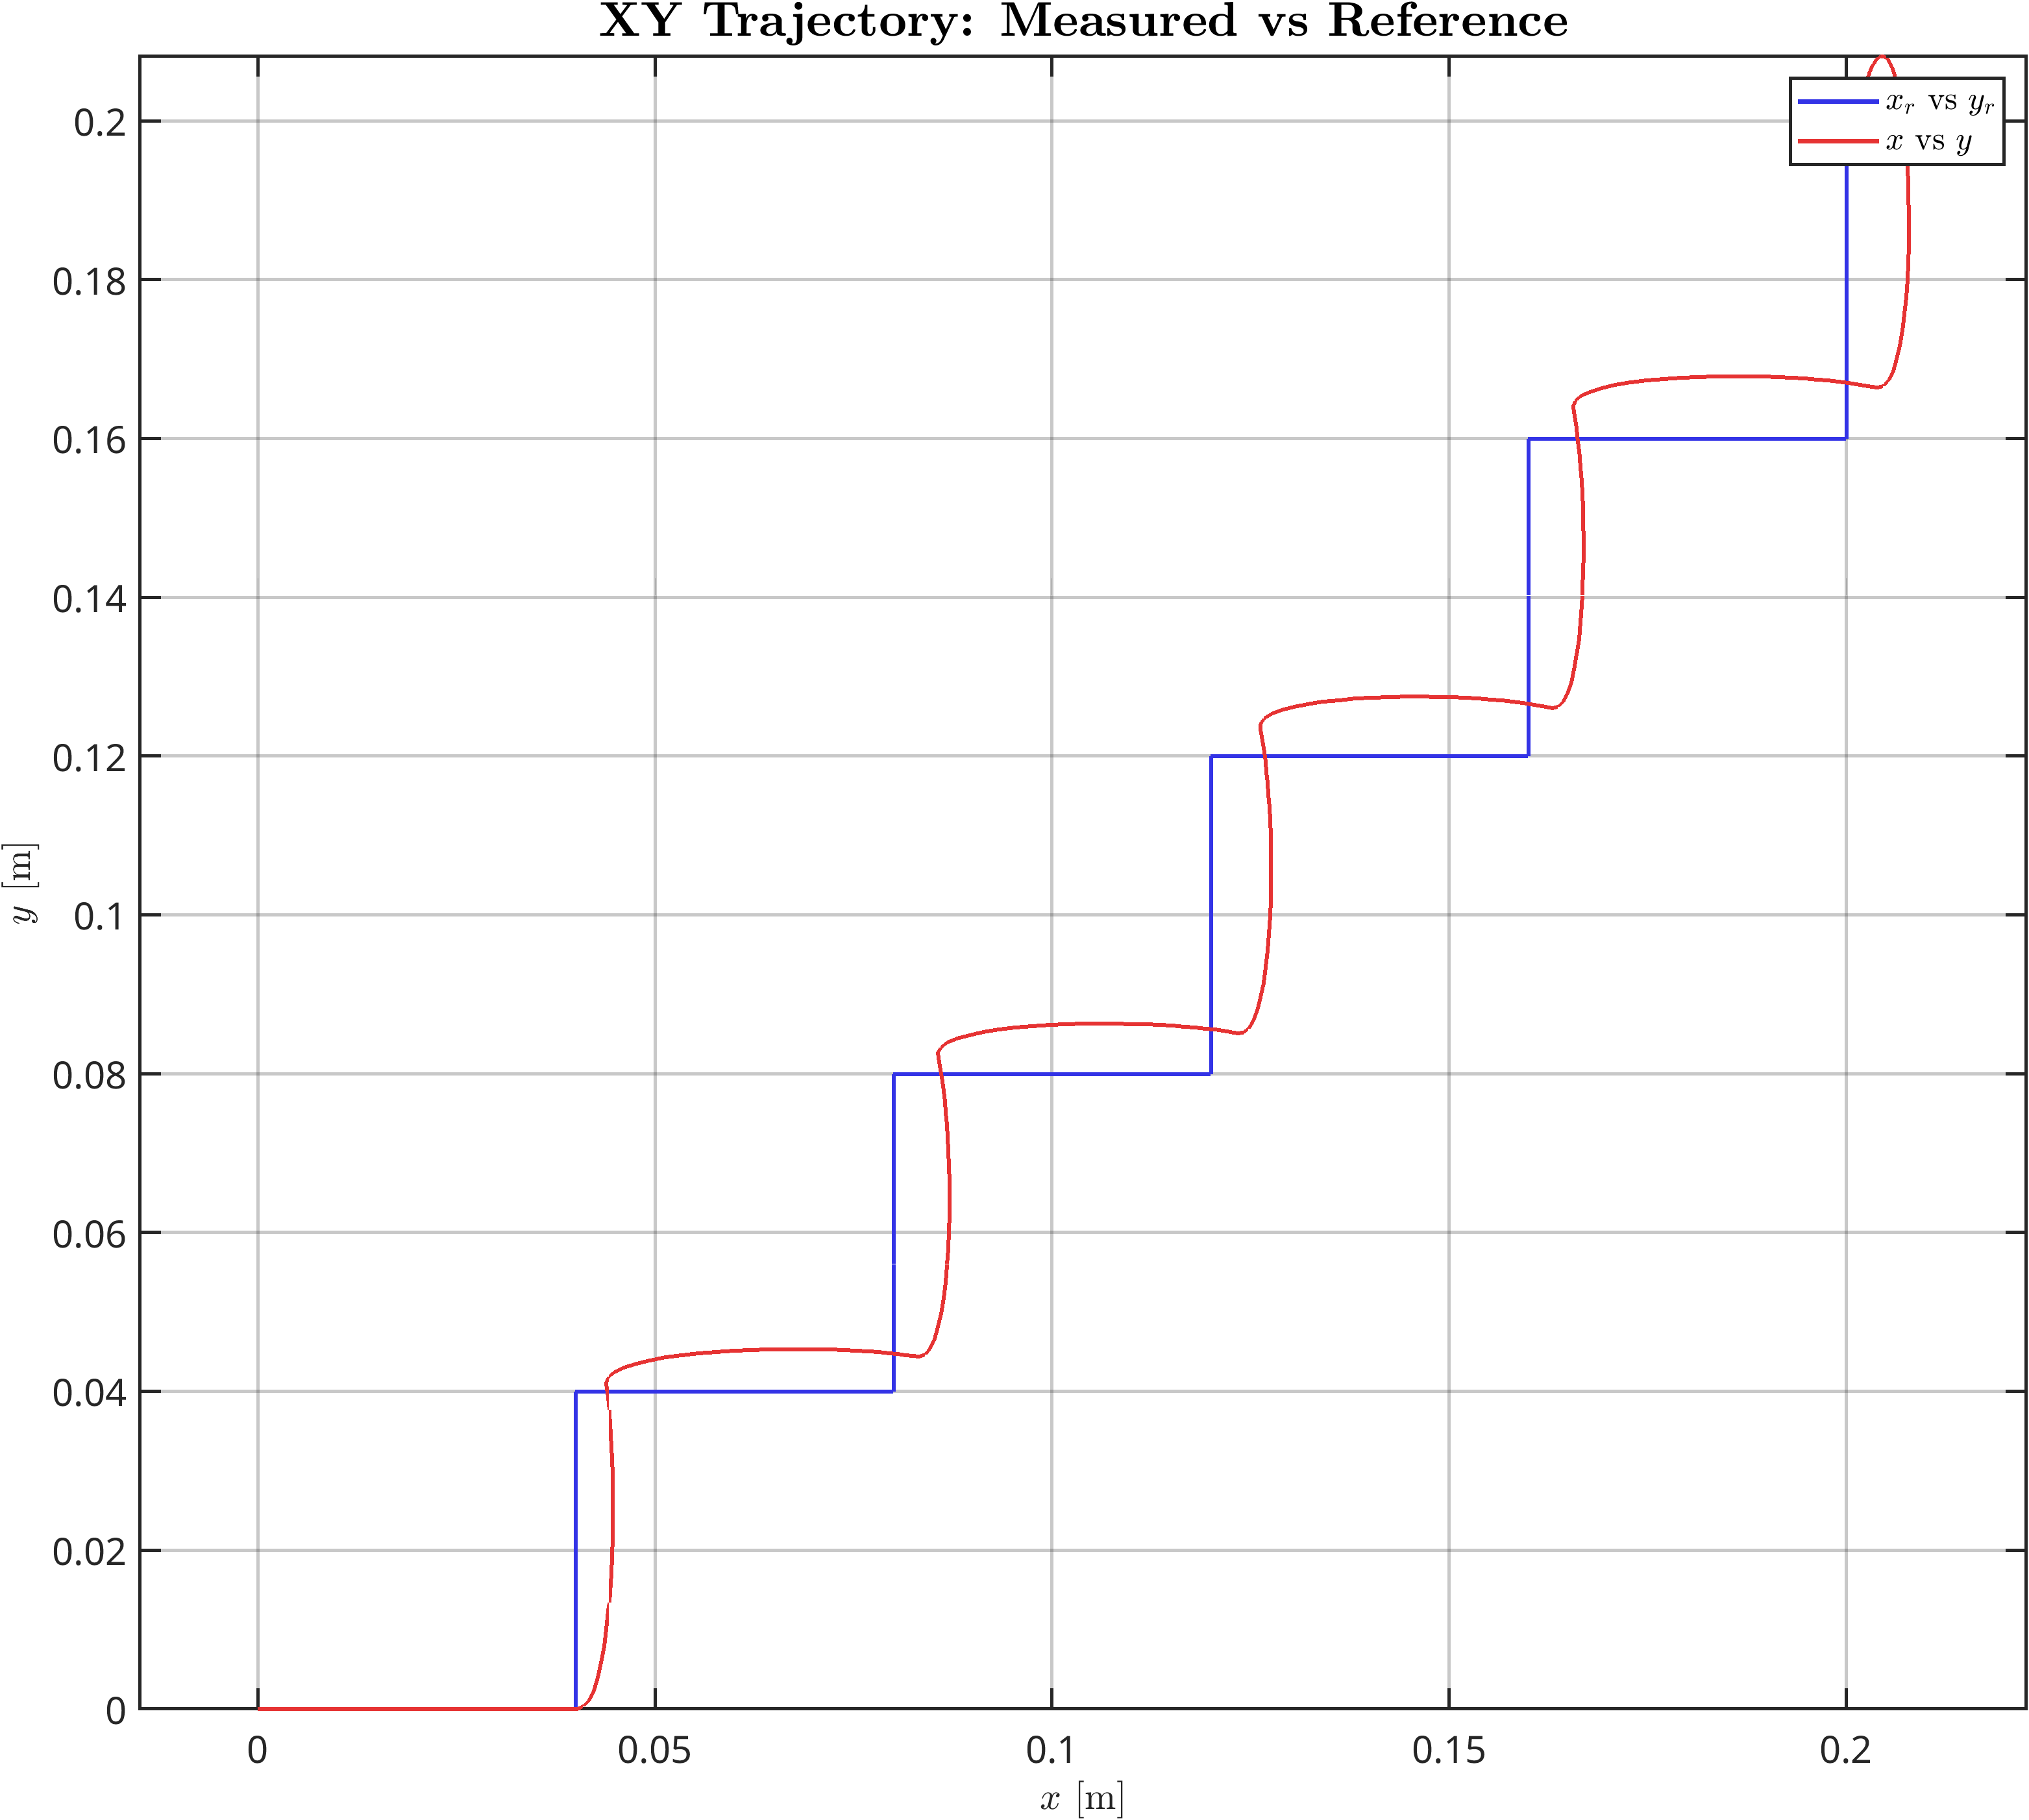
\includegraphics[width=0.7\textwidth]{img/manhattan/5/xy-trajectory}
	\caption{مسیر صفحه‌ای منهتن با زمان کل $5$ ثانیه؛ انحراف فزاینده از مسیر مرجع مشهود است.}
	\label{fig:results-manhattan-5-xy}
\end{figure}

\begin{figure}[htbp]
	\centering
	\subfloat[بهره‌های فازی $X$]{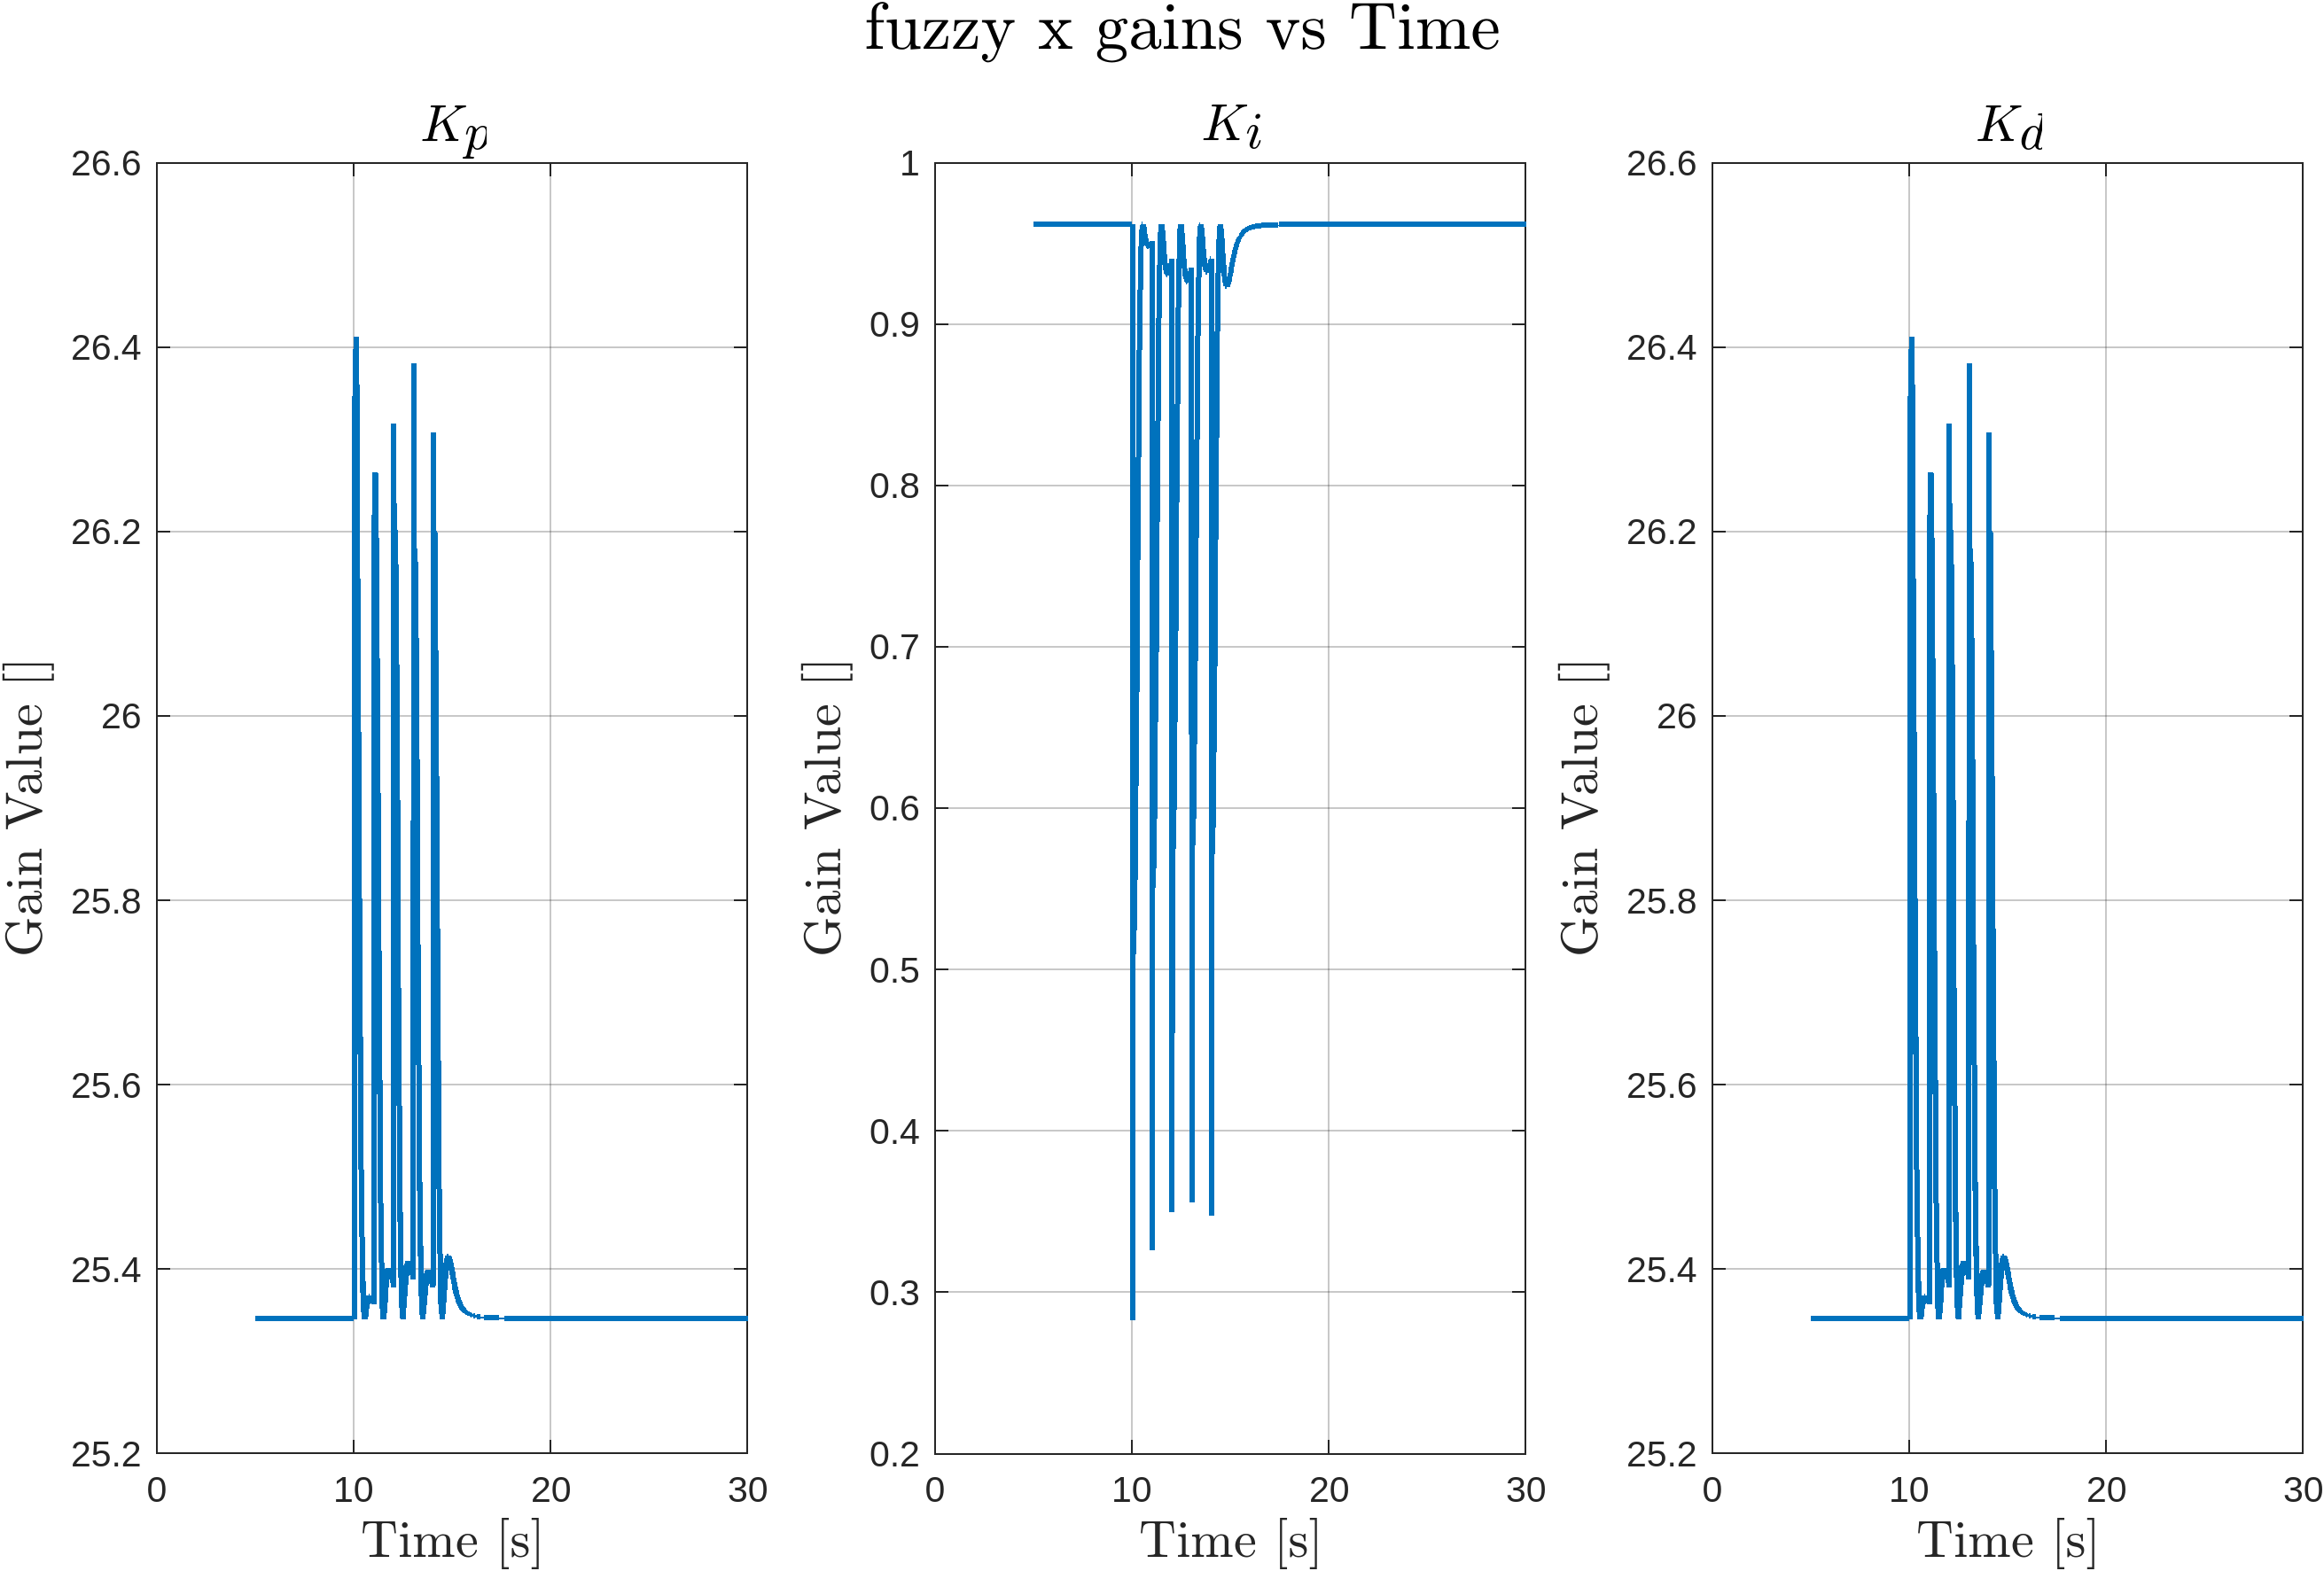
\includegraphics[width=0.48\textwidth]{img/manhattan/5/fuzzy_x_gains}}
	\hfill
	\subfloat[بهره‌های فازی $Y$]{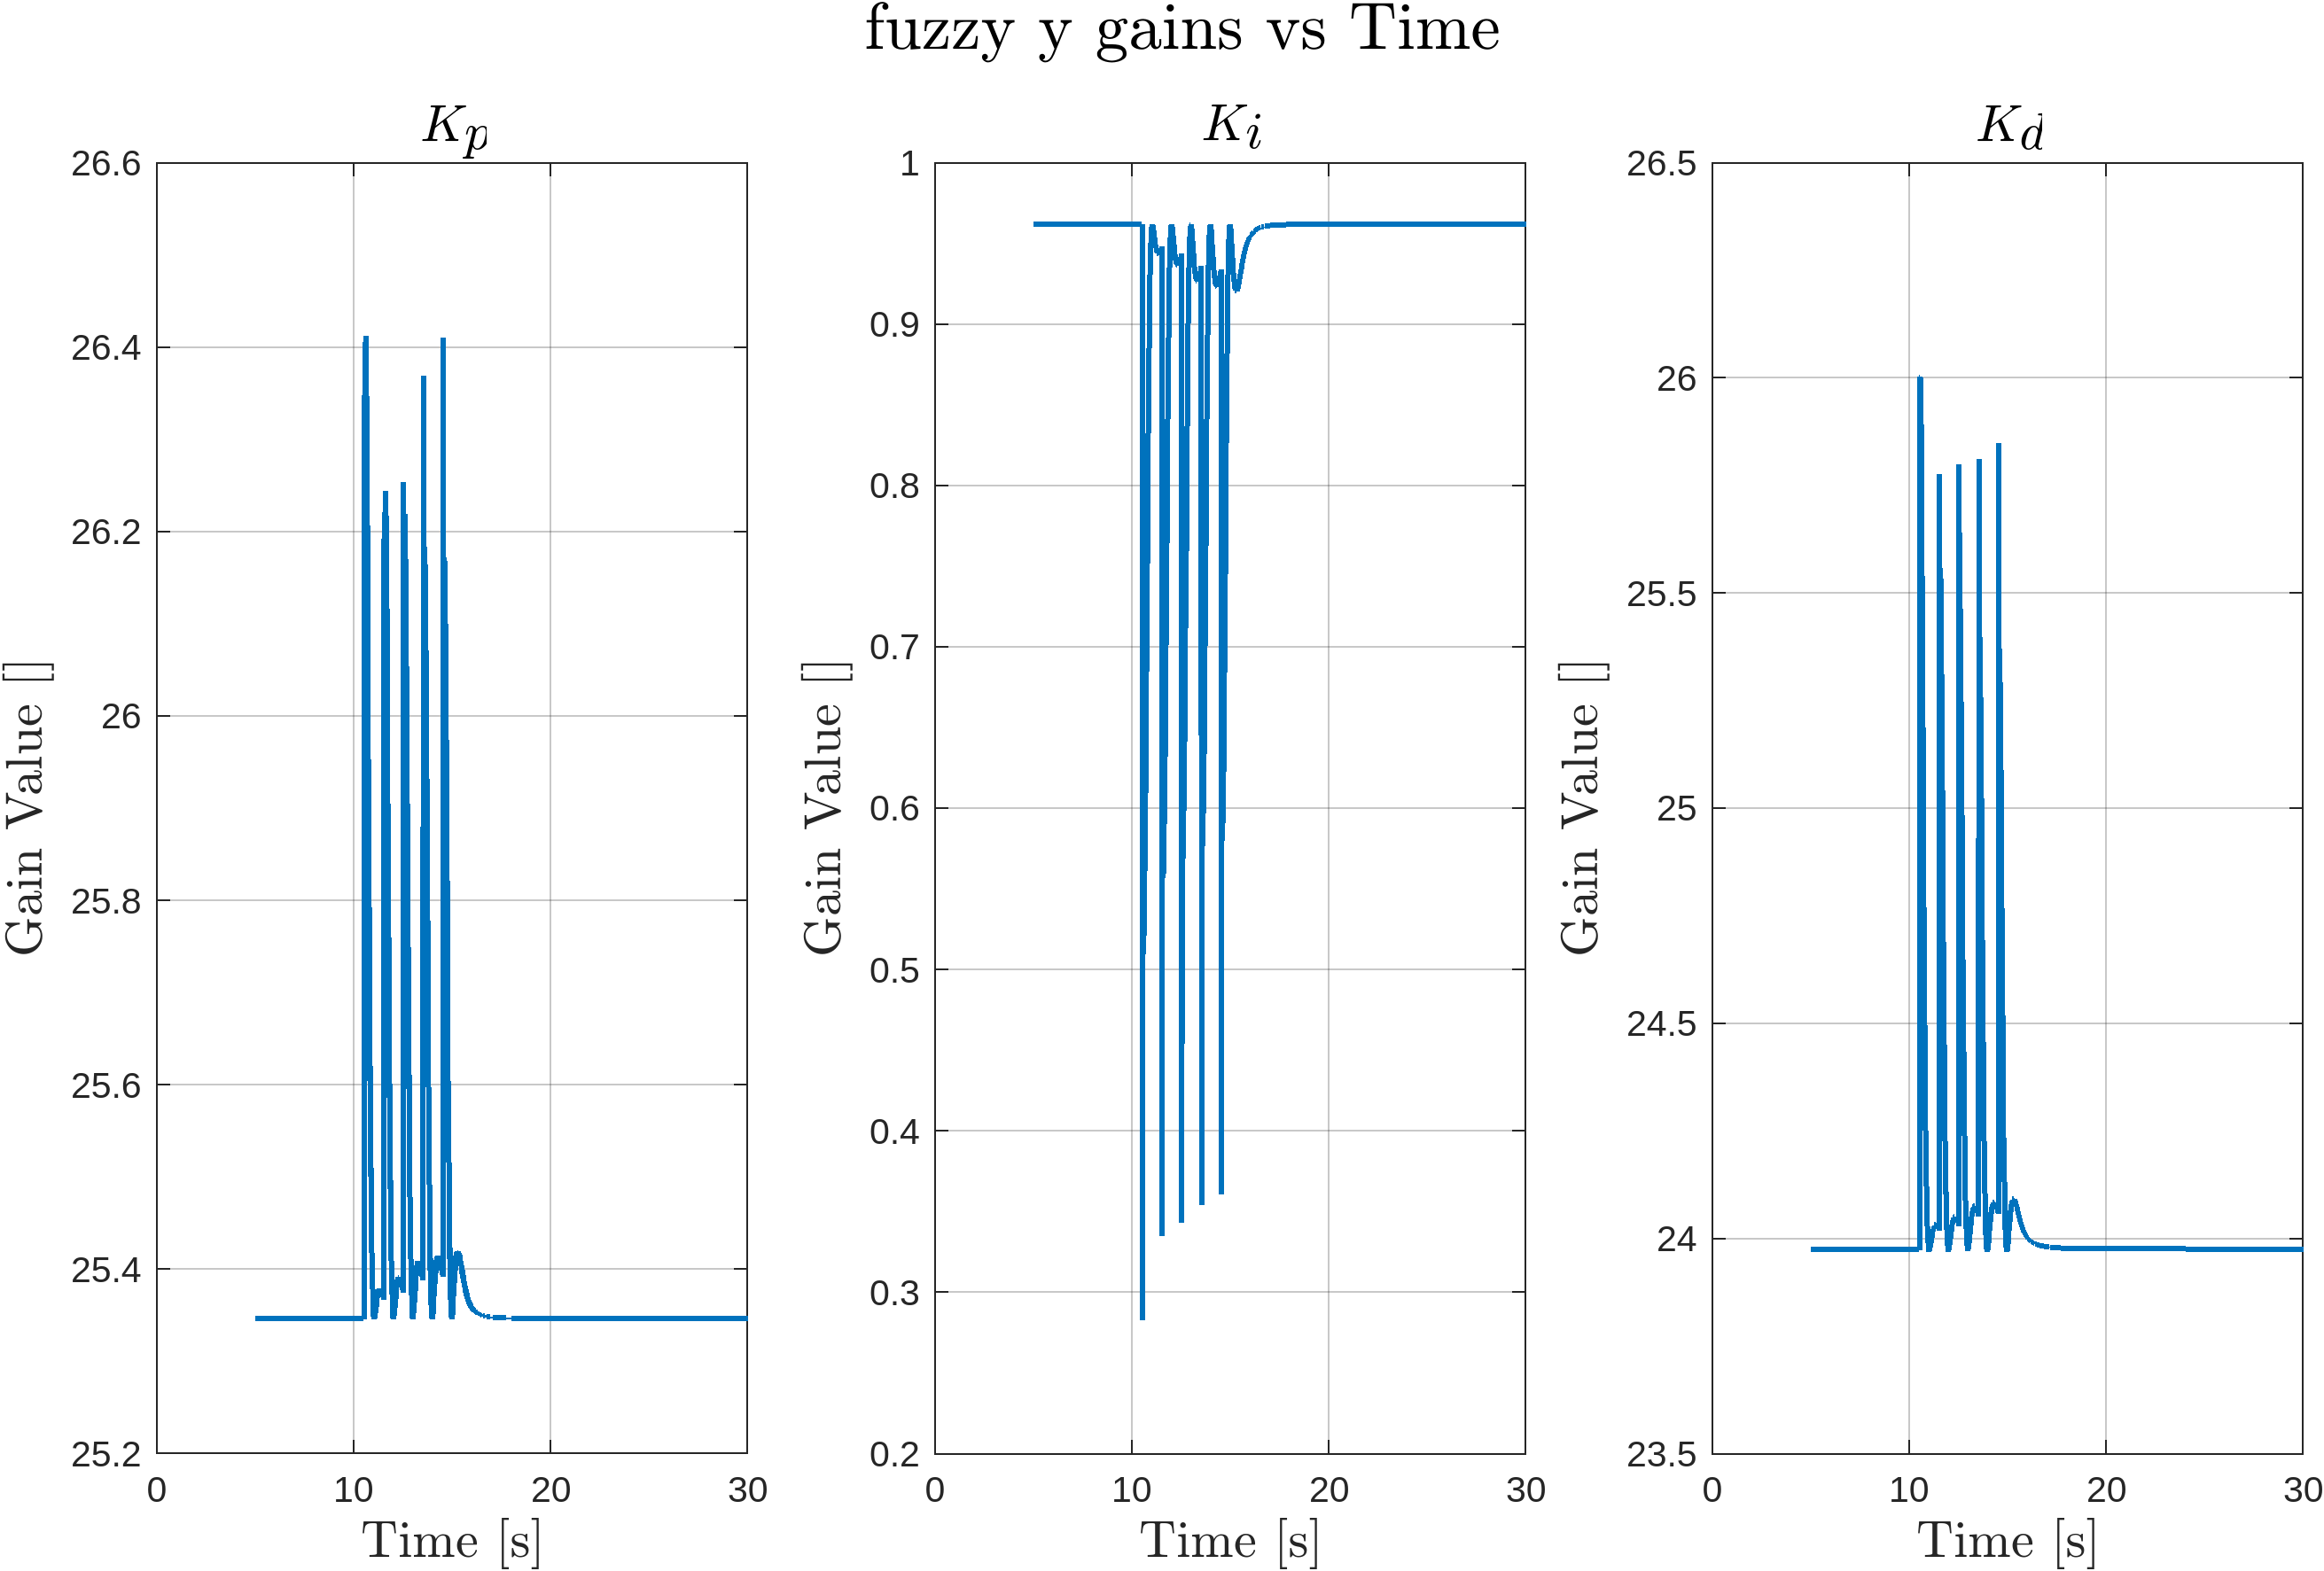
\includegraphics[width=0.48\textwidth]{img/manhattan/5/fuzzy_y_gains}}
	\caption{تغییرات ضرایب کنترلی فازی در آزمون $5$ ثانیه‌ای}
	\label{fig:results-manhattan-5-fuzzy}
\end{figure}

\subsubsection{آزمون با زمان $T_{\text{total}} = 10$ ثانیه}
\label{subsubsec:results-manhattan-10}
با دو برابر شدن زمان کل به $10$ ثانیه ($t_{\text{seg}} = 1.0$ ثانیه)، کیفیت ردیابی به‌طور چشمگیری بهبود می‌یابد. شکل \ref{fig:results-manhattan-10-xy} نشان می‌دهد که مسیر حرکتی به مراتب به مسیر مرجع نزدیک‌تر شده است. در انتهای بیشتر پله‌ها، بخش متحرک به همسایگی نقطه‌ی مطلوب رسیده و خطای باقی‌مانده از نظر بصری بسیار کوچک و به زحمت قابل تشخیص است. با این وجود، هنوز انباشتگی جزئی خطا در طول پله‌های متوالی رخ می‌دهد، اما میزان آن به مراتب کمتر از آزمون ۵ ثانیه‌ای است. کنترل‌کننده‌ی فازی در این حالت فرصت کافی برای میراسازی نوسانات و بازگشت بهره‌های خود به مقادیر میانی را پیدا می‌کند (شکل \ref{fig:results-manhattan-10-fuzzy}).

\begin{figure}[htbp]
	\centering
	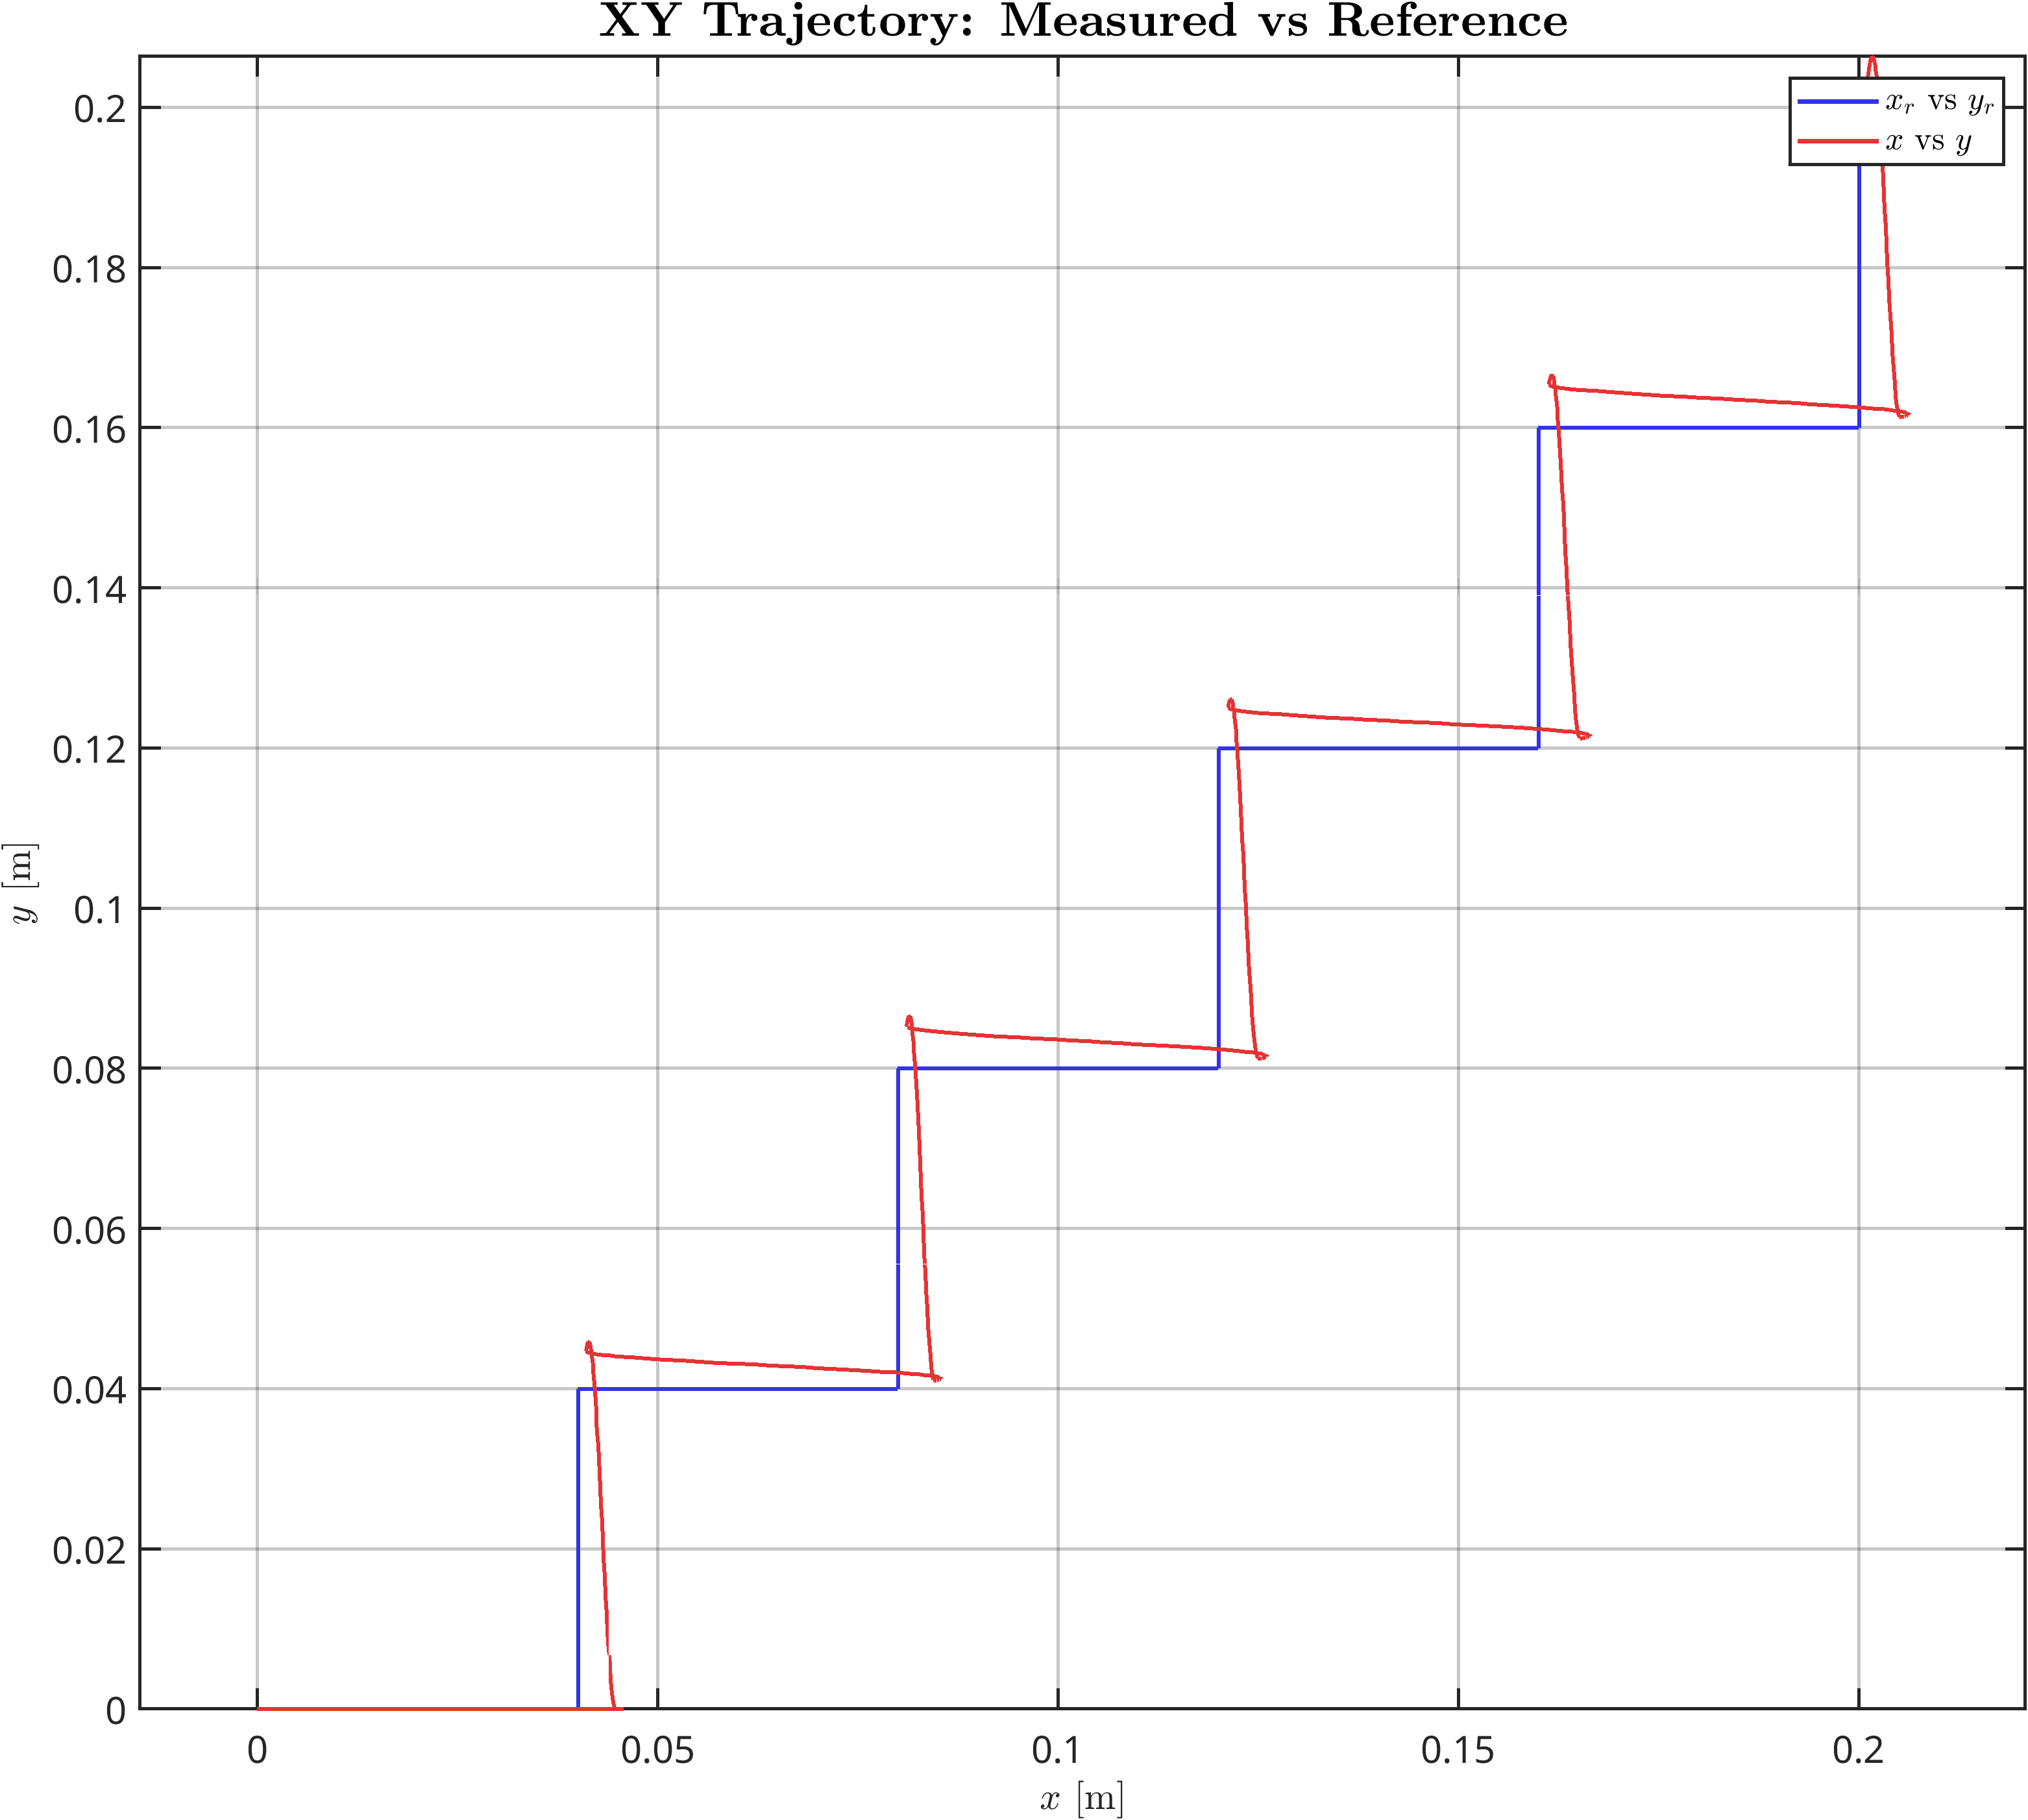
\includegraphics[width=0.7\textwidth]{img/manhattan/10/xy-trajectory}
	\caption{مسیر صفحه‌ای منهتن با زمان کل $10$ ثانیه؛ انحراف از مرجع به شدت کاهش یافته است.}
	\label{fig:results-manhattan-10-xy}
\end{figure}

\begin{figure}[htbp]
	\centering
	\subfloat[بهره‌های فازی $X$]{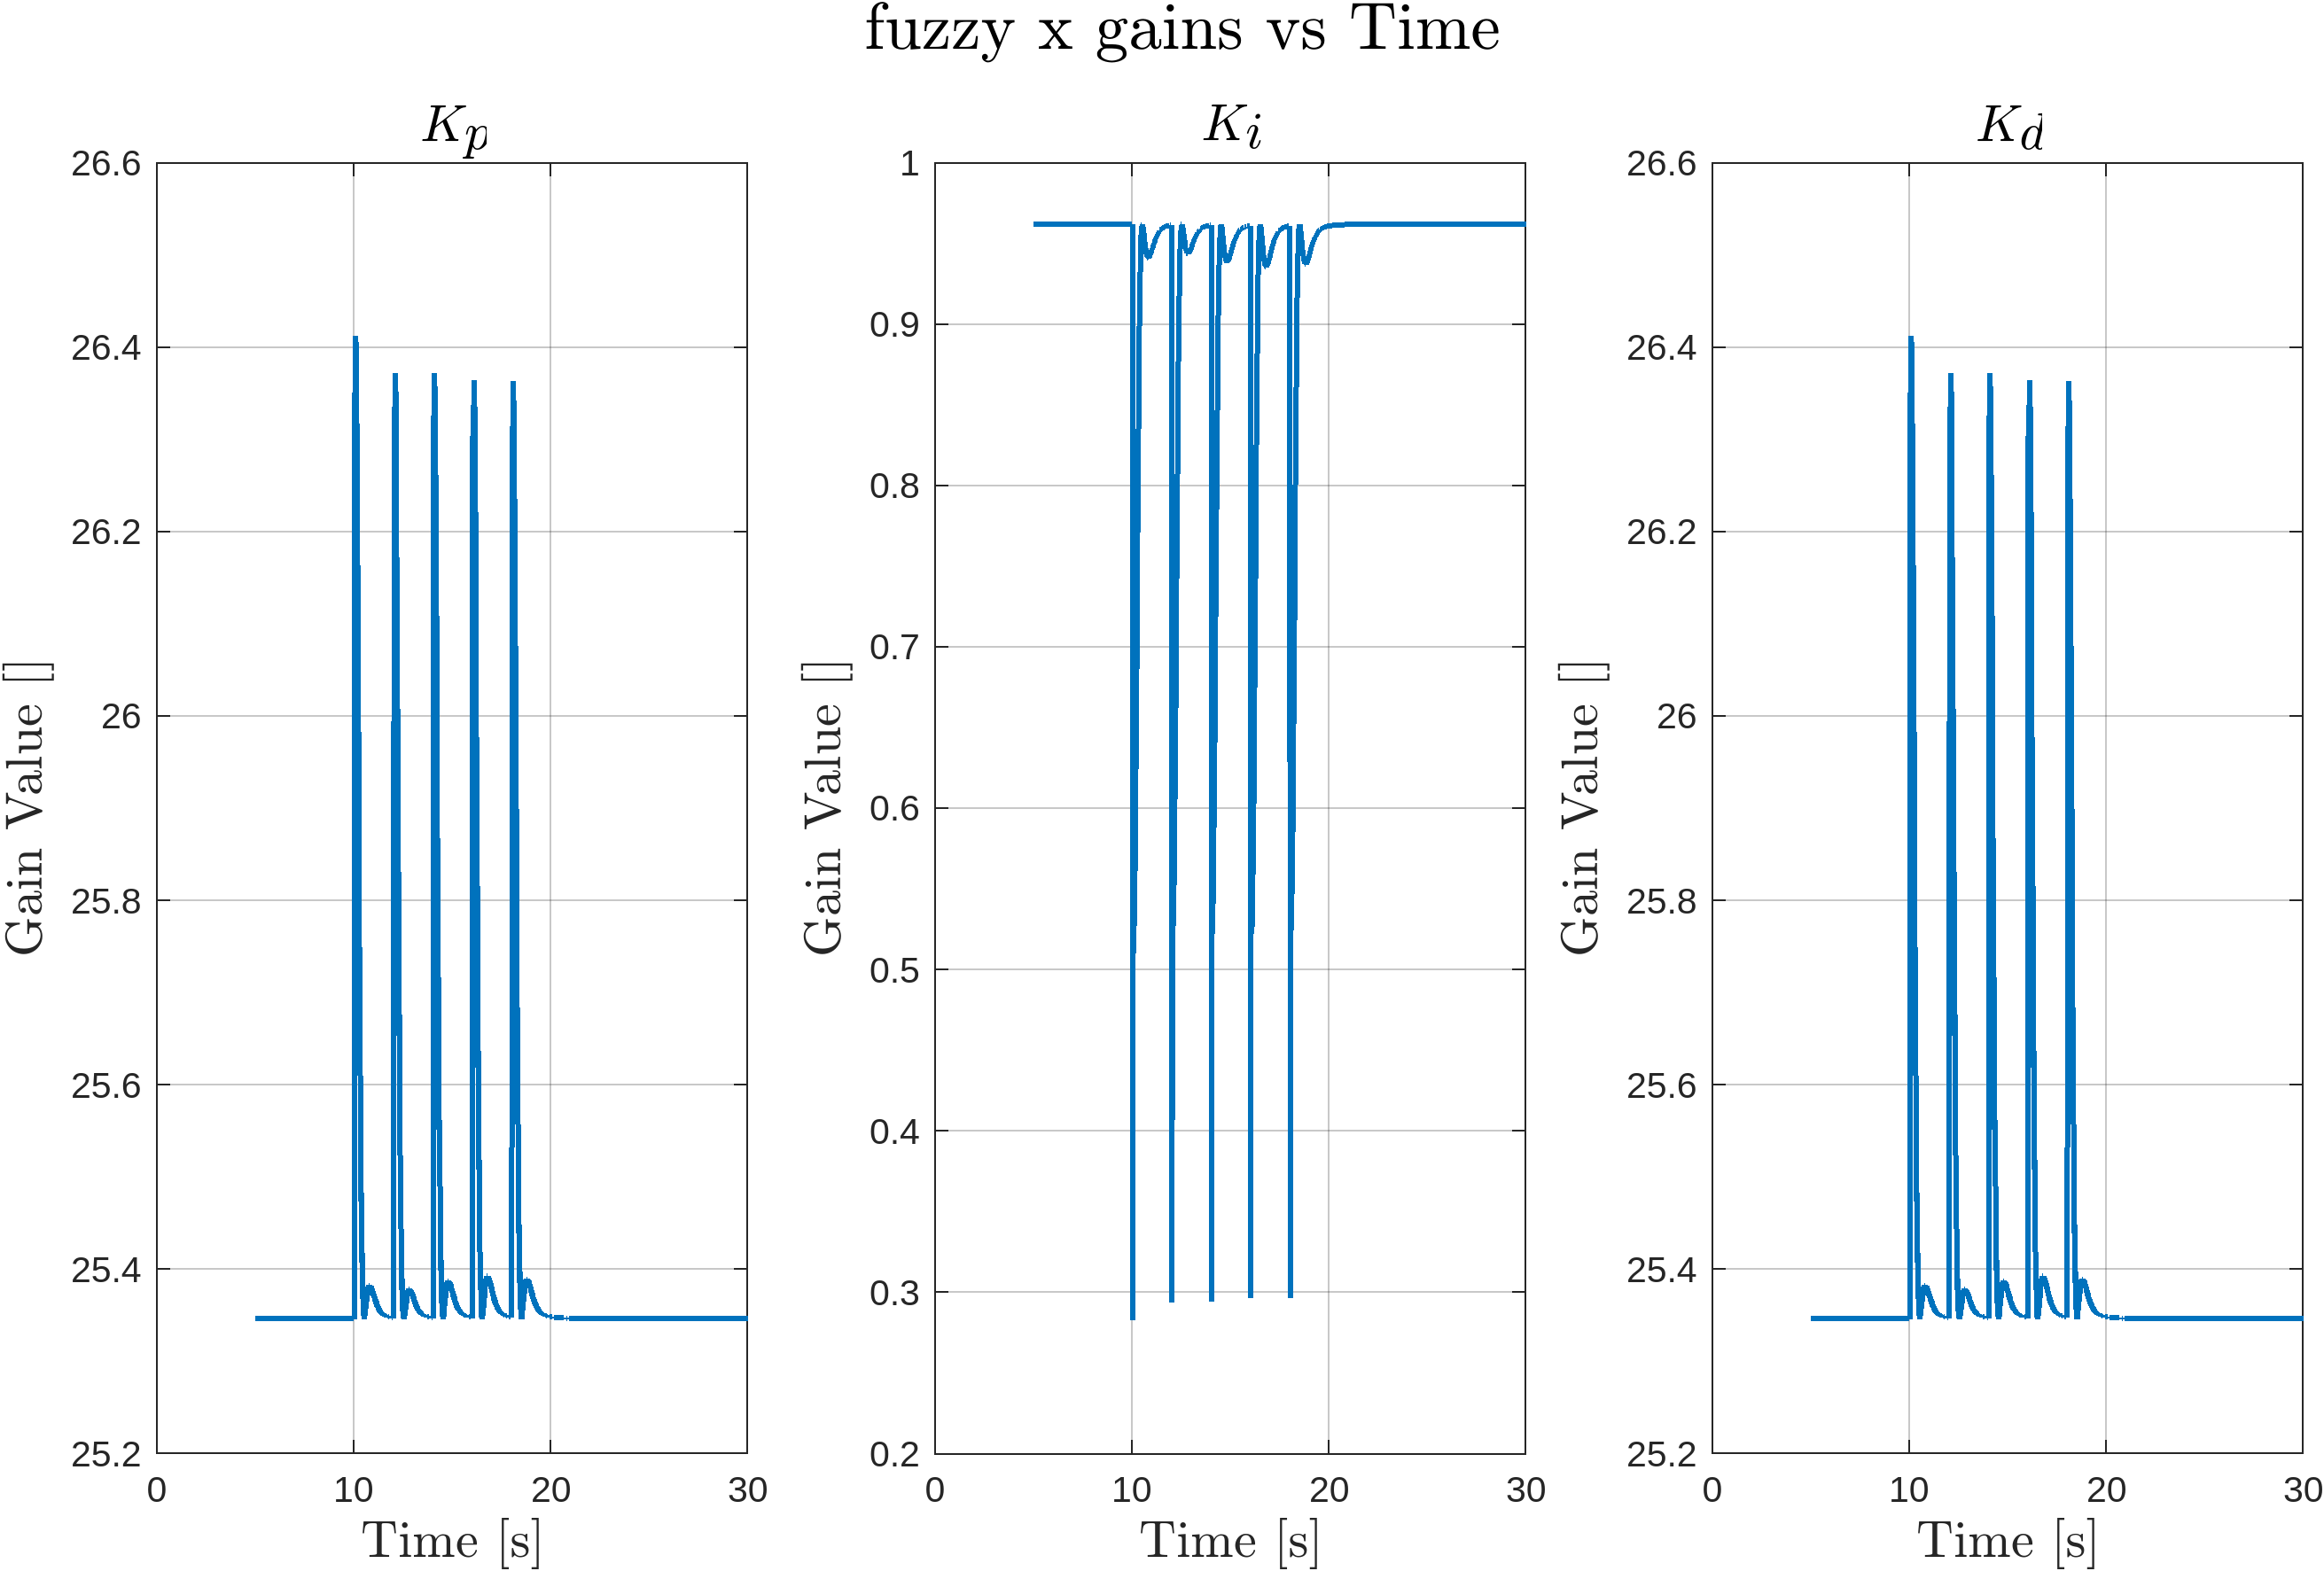
\includegraphics[width=0.48\textwidth]{img/manhattan/10/fuzzy_x_gains}}
	\hfill
	\subfloat[بهره‌های فازی $Y$]{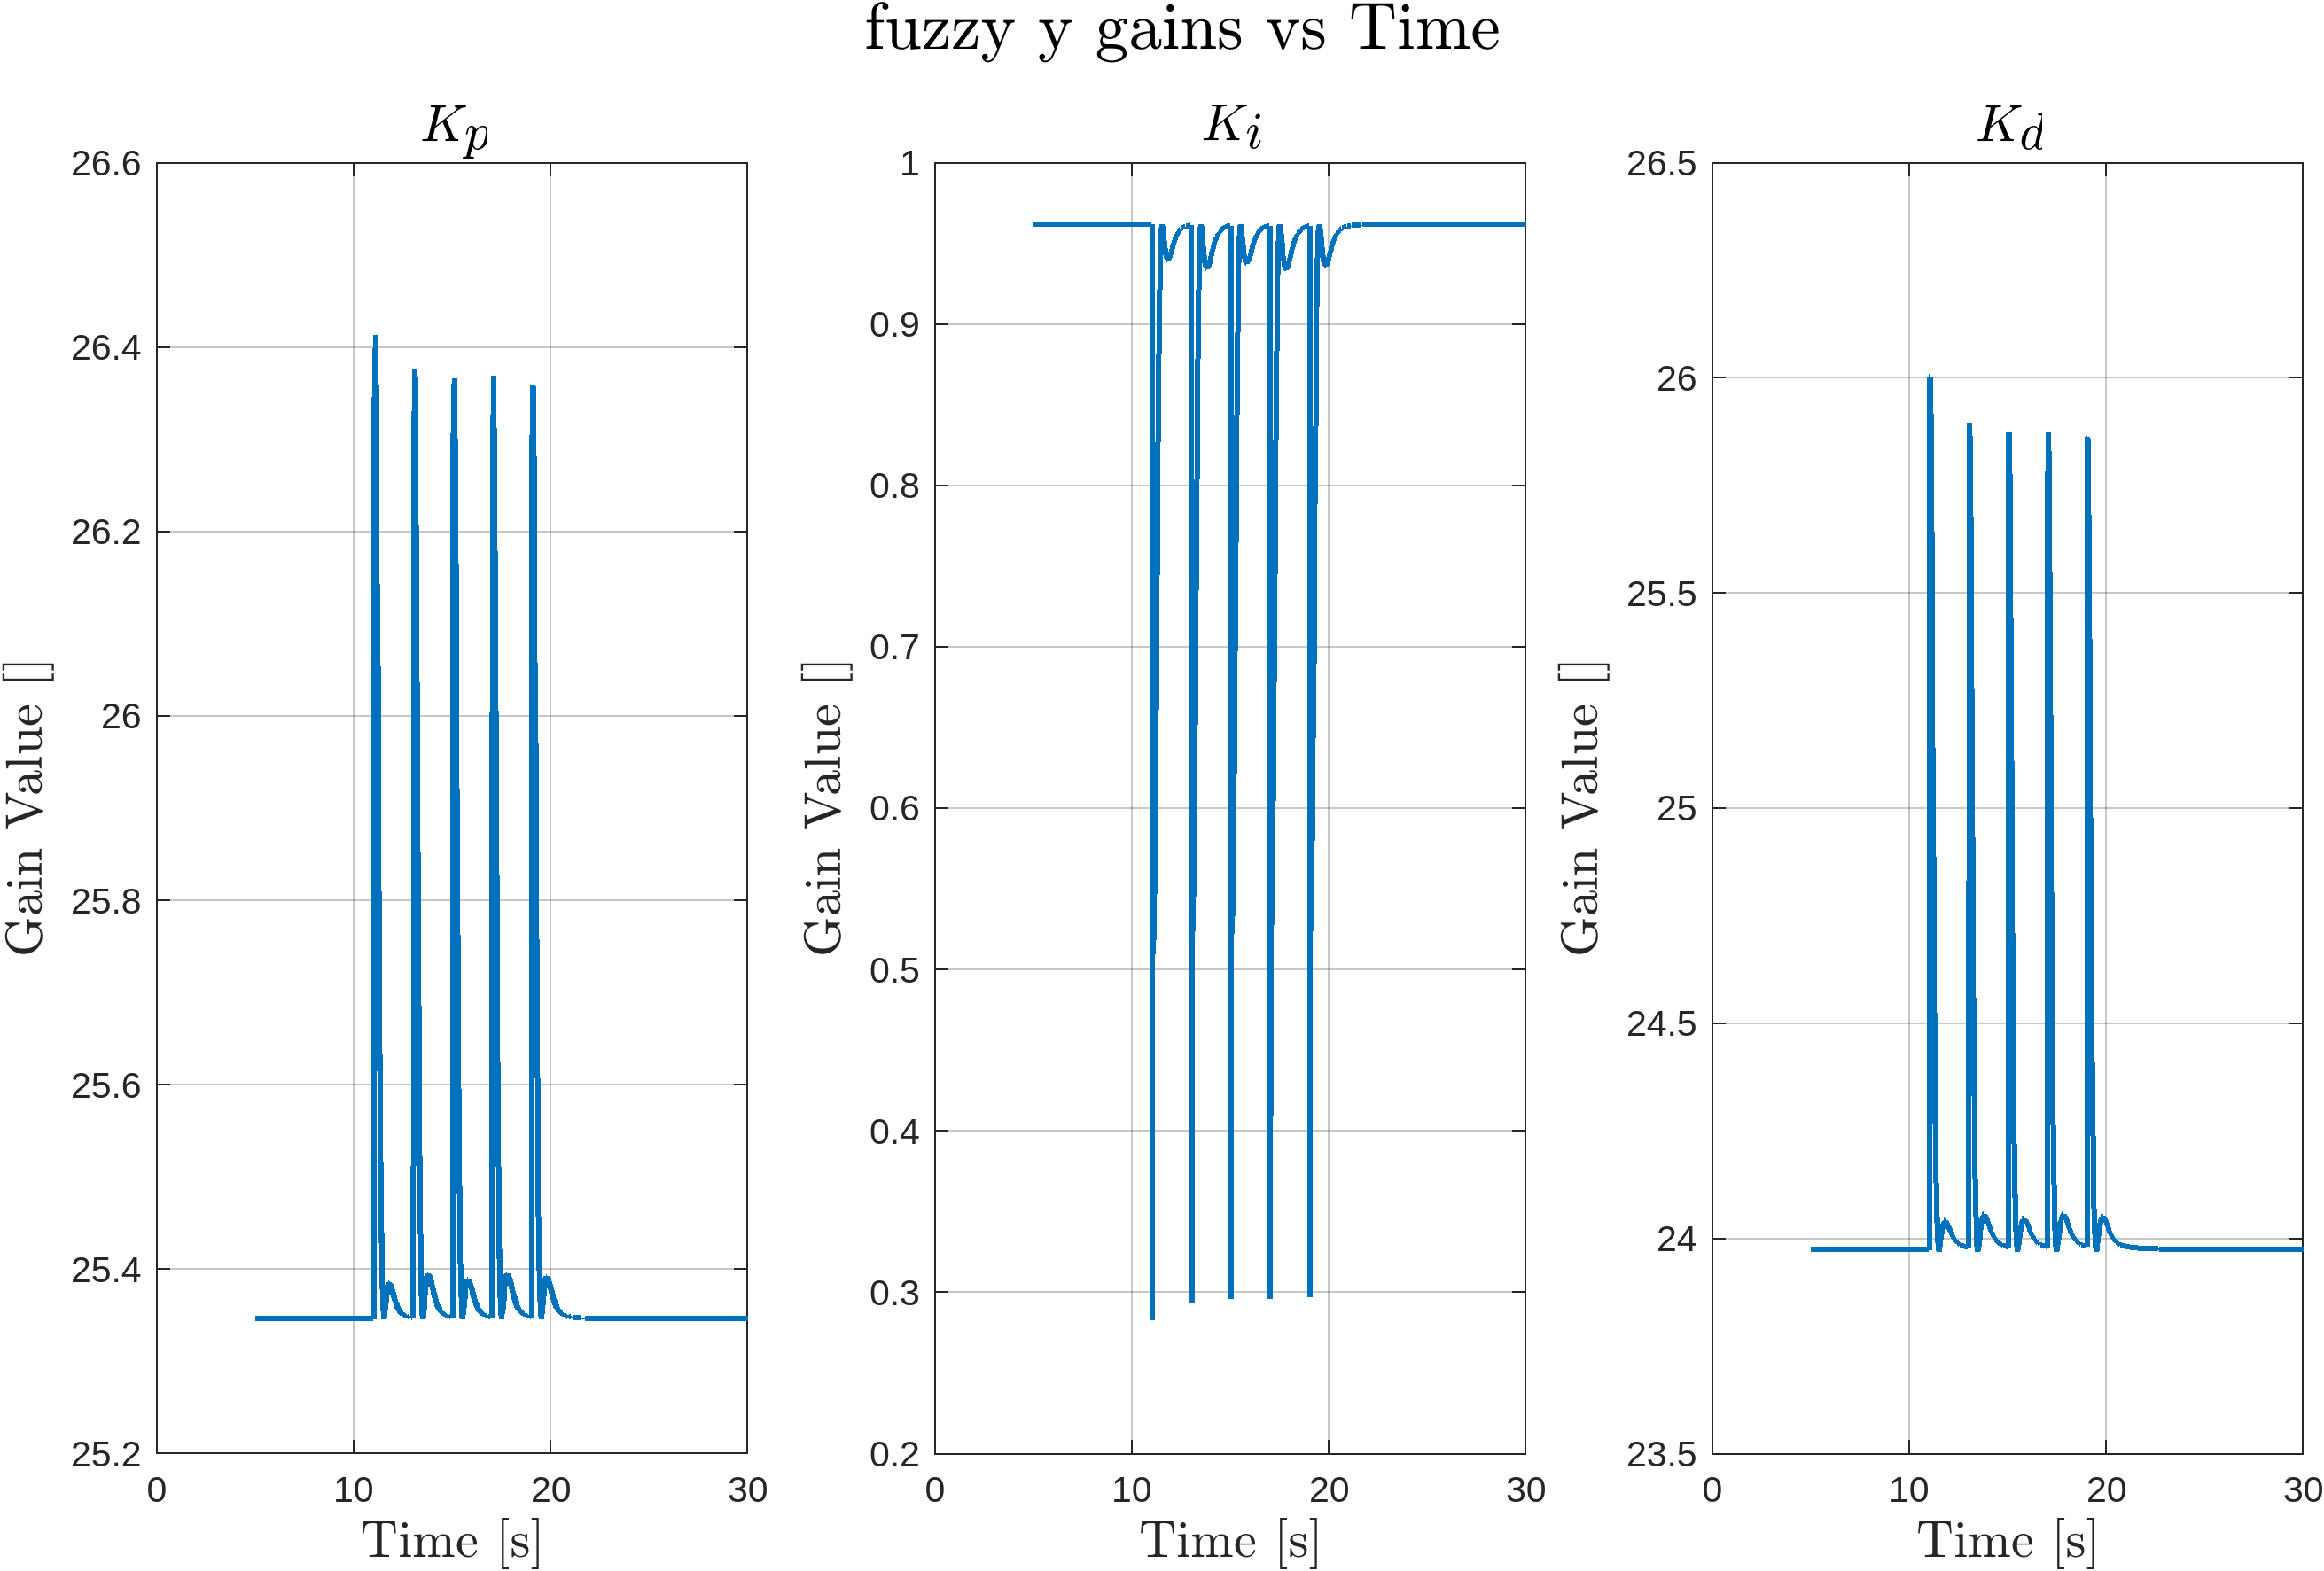
\includegraphics[width=0.48\textwidth]{img/manhattan/10/fuzzy_y_gains}}
	\caption{تغییرات ضرایب کنترلی فازی در آزمون $10$ ثانیه‌ای}
	\label{fig:results-manhattan-10-fuzzy}
\end{figure}

\subsubsection{آزمون با زمان $T_{\text{total}} = 15$ ثانیه}
\label{subsubsec:results-manhattan-15}
در کندترین حالت ($t_{\text{seg}} = 1.5$ ثانیه)، سیستم عملکردی نزدیک به ایده‌آل از خود نشان می‌دهد. شکل \ref{fig:results-manhattan-15-xy} گواه آن است که مسیر پیموده‌شده تقریباً به طور کامل بر مسیر مرجع منطبق است. در پایان هر پله، پاسخ به‌طور کامل به مقدار مطلوب هم‌گرا شده و خطای حالت ماندگار عملاً صفر است. در نتیجه، پدیده‌ی انباشتگی خطا به کلی حذف شده و تمامی پله‌ها شکلی یکسان از ردیابی دقیق را به نمایش می‌گذارند. سیگنال‌های خطای محورهای $X$ و $Y$ (شکل \ref{fig:results-manhattan-15-error}) نشان می‌دهند که پس از هر جهش، خطا به سرعت و بدون فراجهش اضافی به صفر بازمی‌گردد. این عملکرد، ظرفیت سیستم را برای کاربری‌های دقیق که سرعت در آنها اولویت نیست، تأیید می‌کند.

\begin{figure}[htbp]
	\centering
	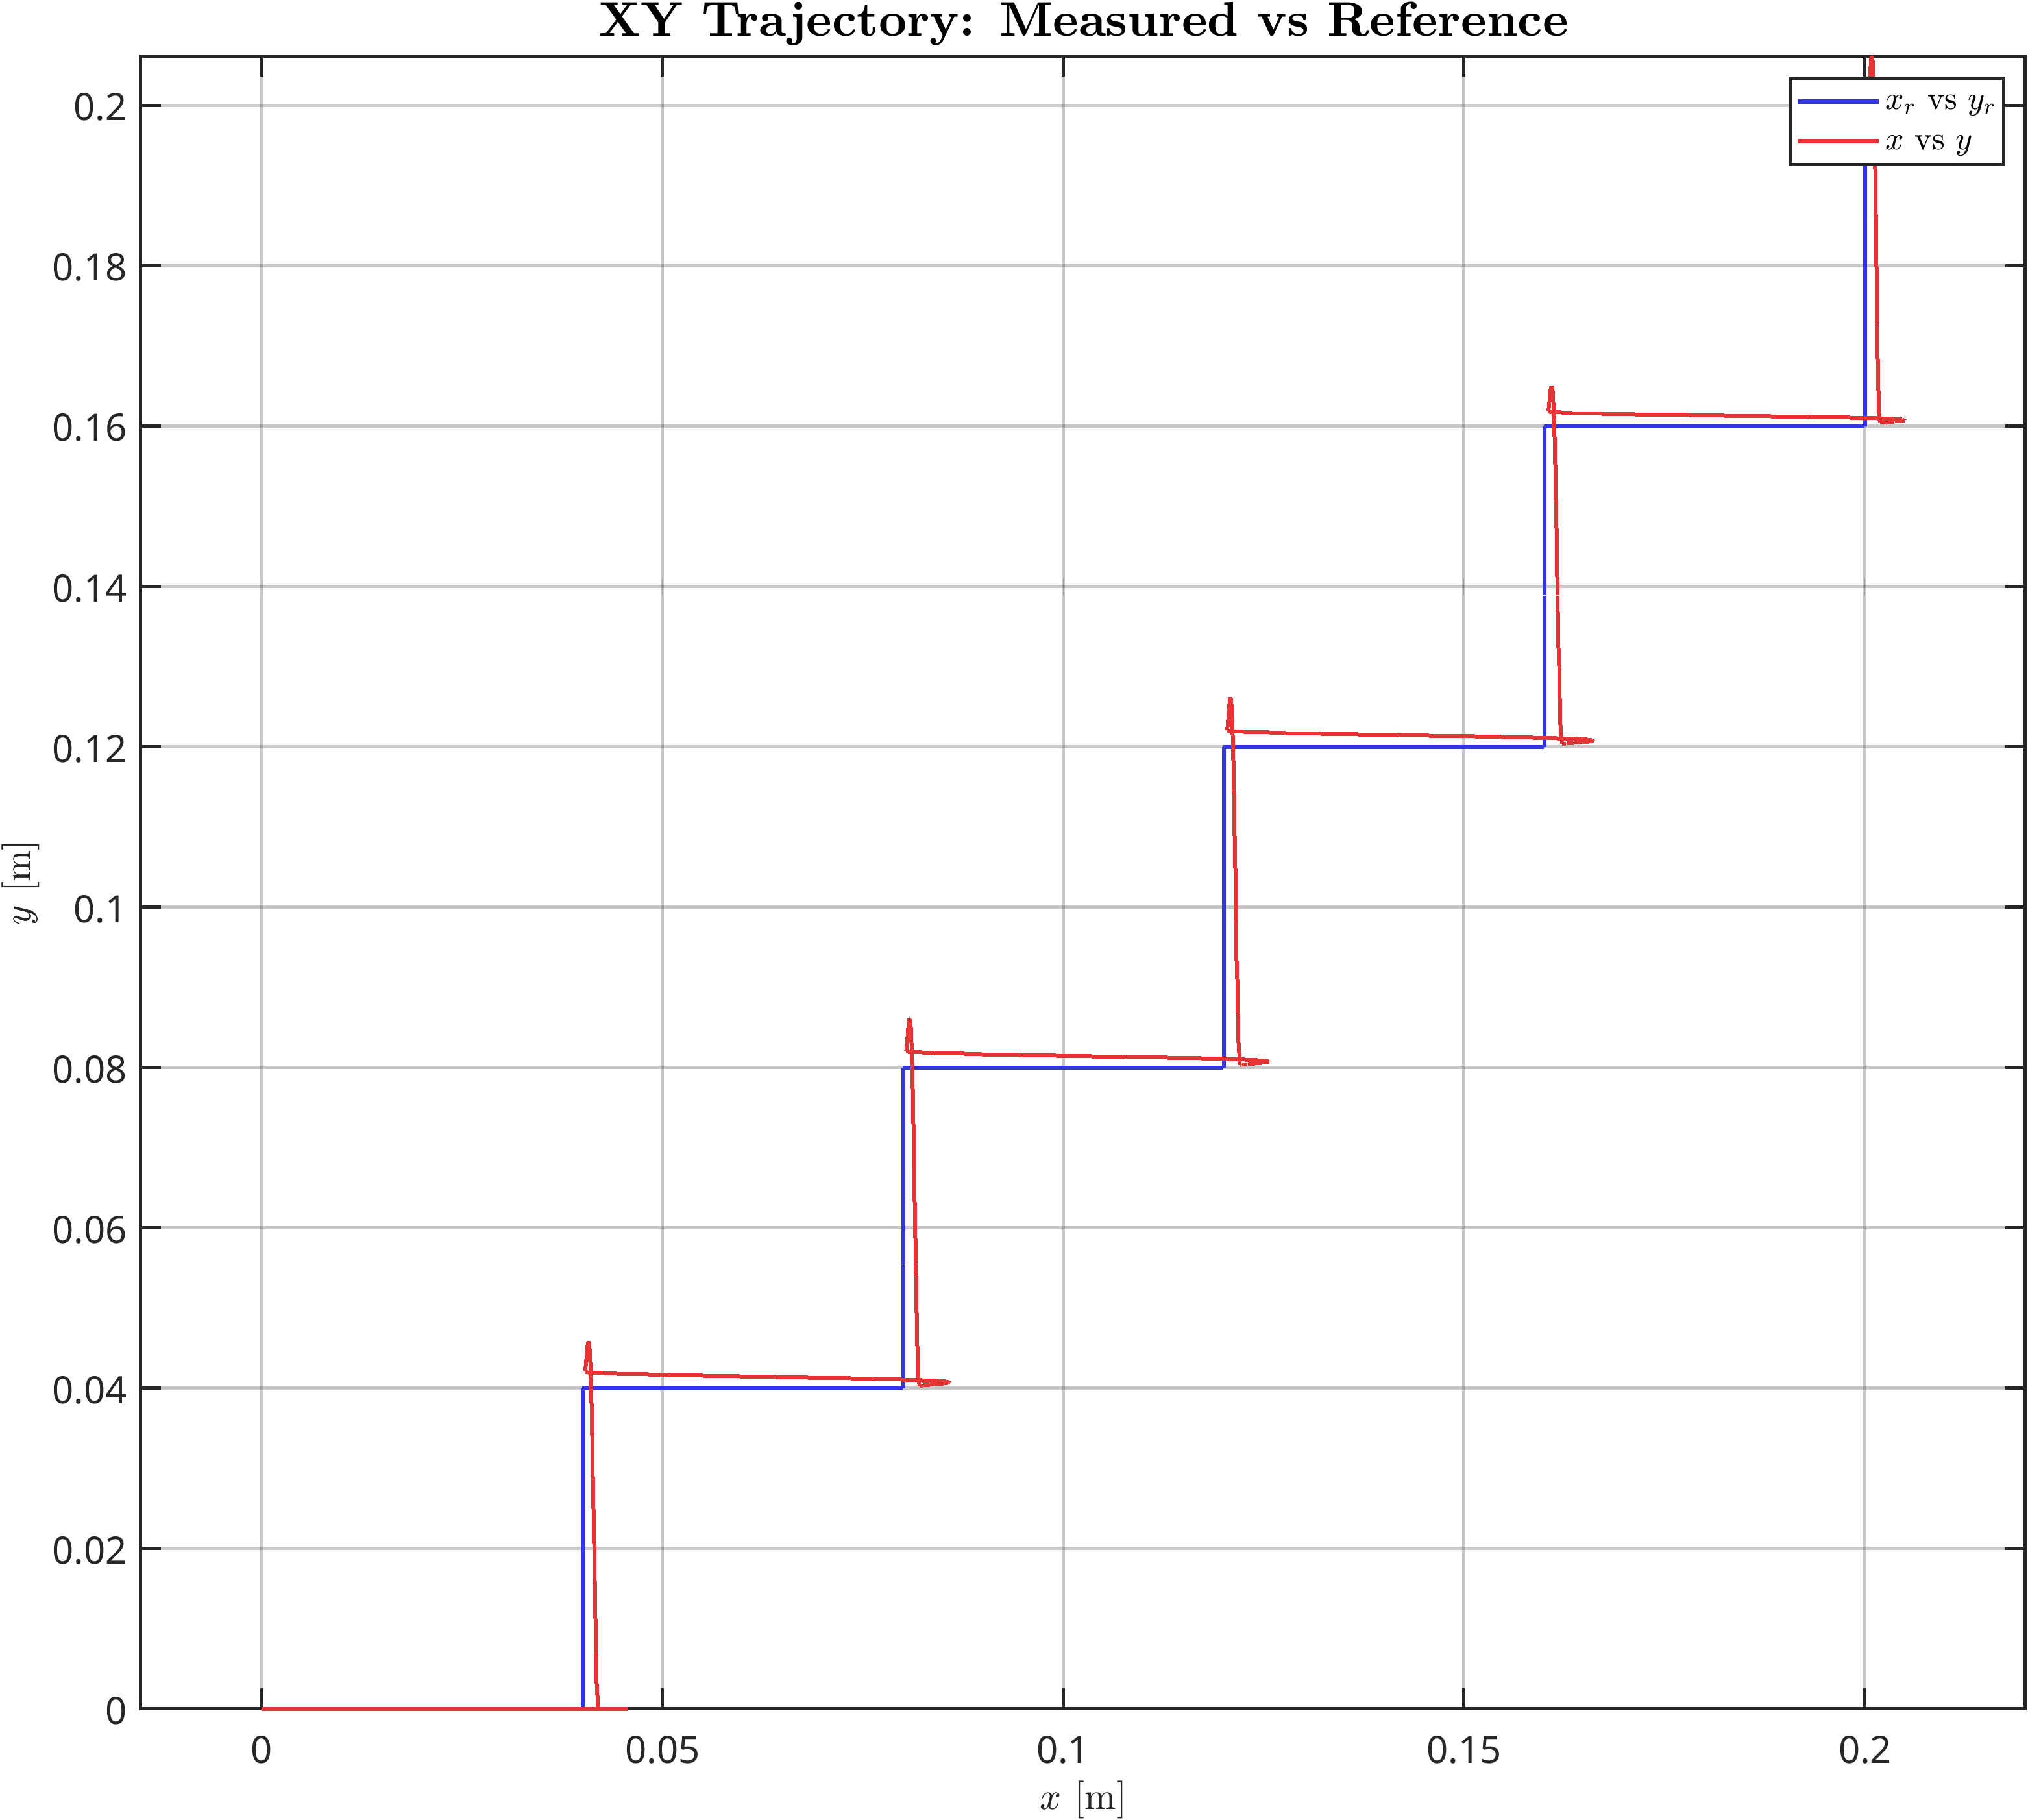
\includegraphics[width=0.7\textwidth]{img/manhattan/15/xy-trajectory}
	\caption{مسیر صفحه‌ای منهتن با زمان کل $15$ ثانیه؛ انطباق کامل با مسیر مرجع حاصل شده است.}
	\label{fig:results-manhattan-15-xy}
\end{figure}

\begin{figure}[htbp]
	\centering
	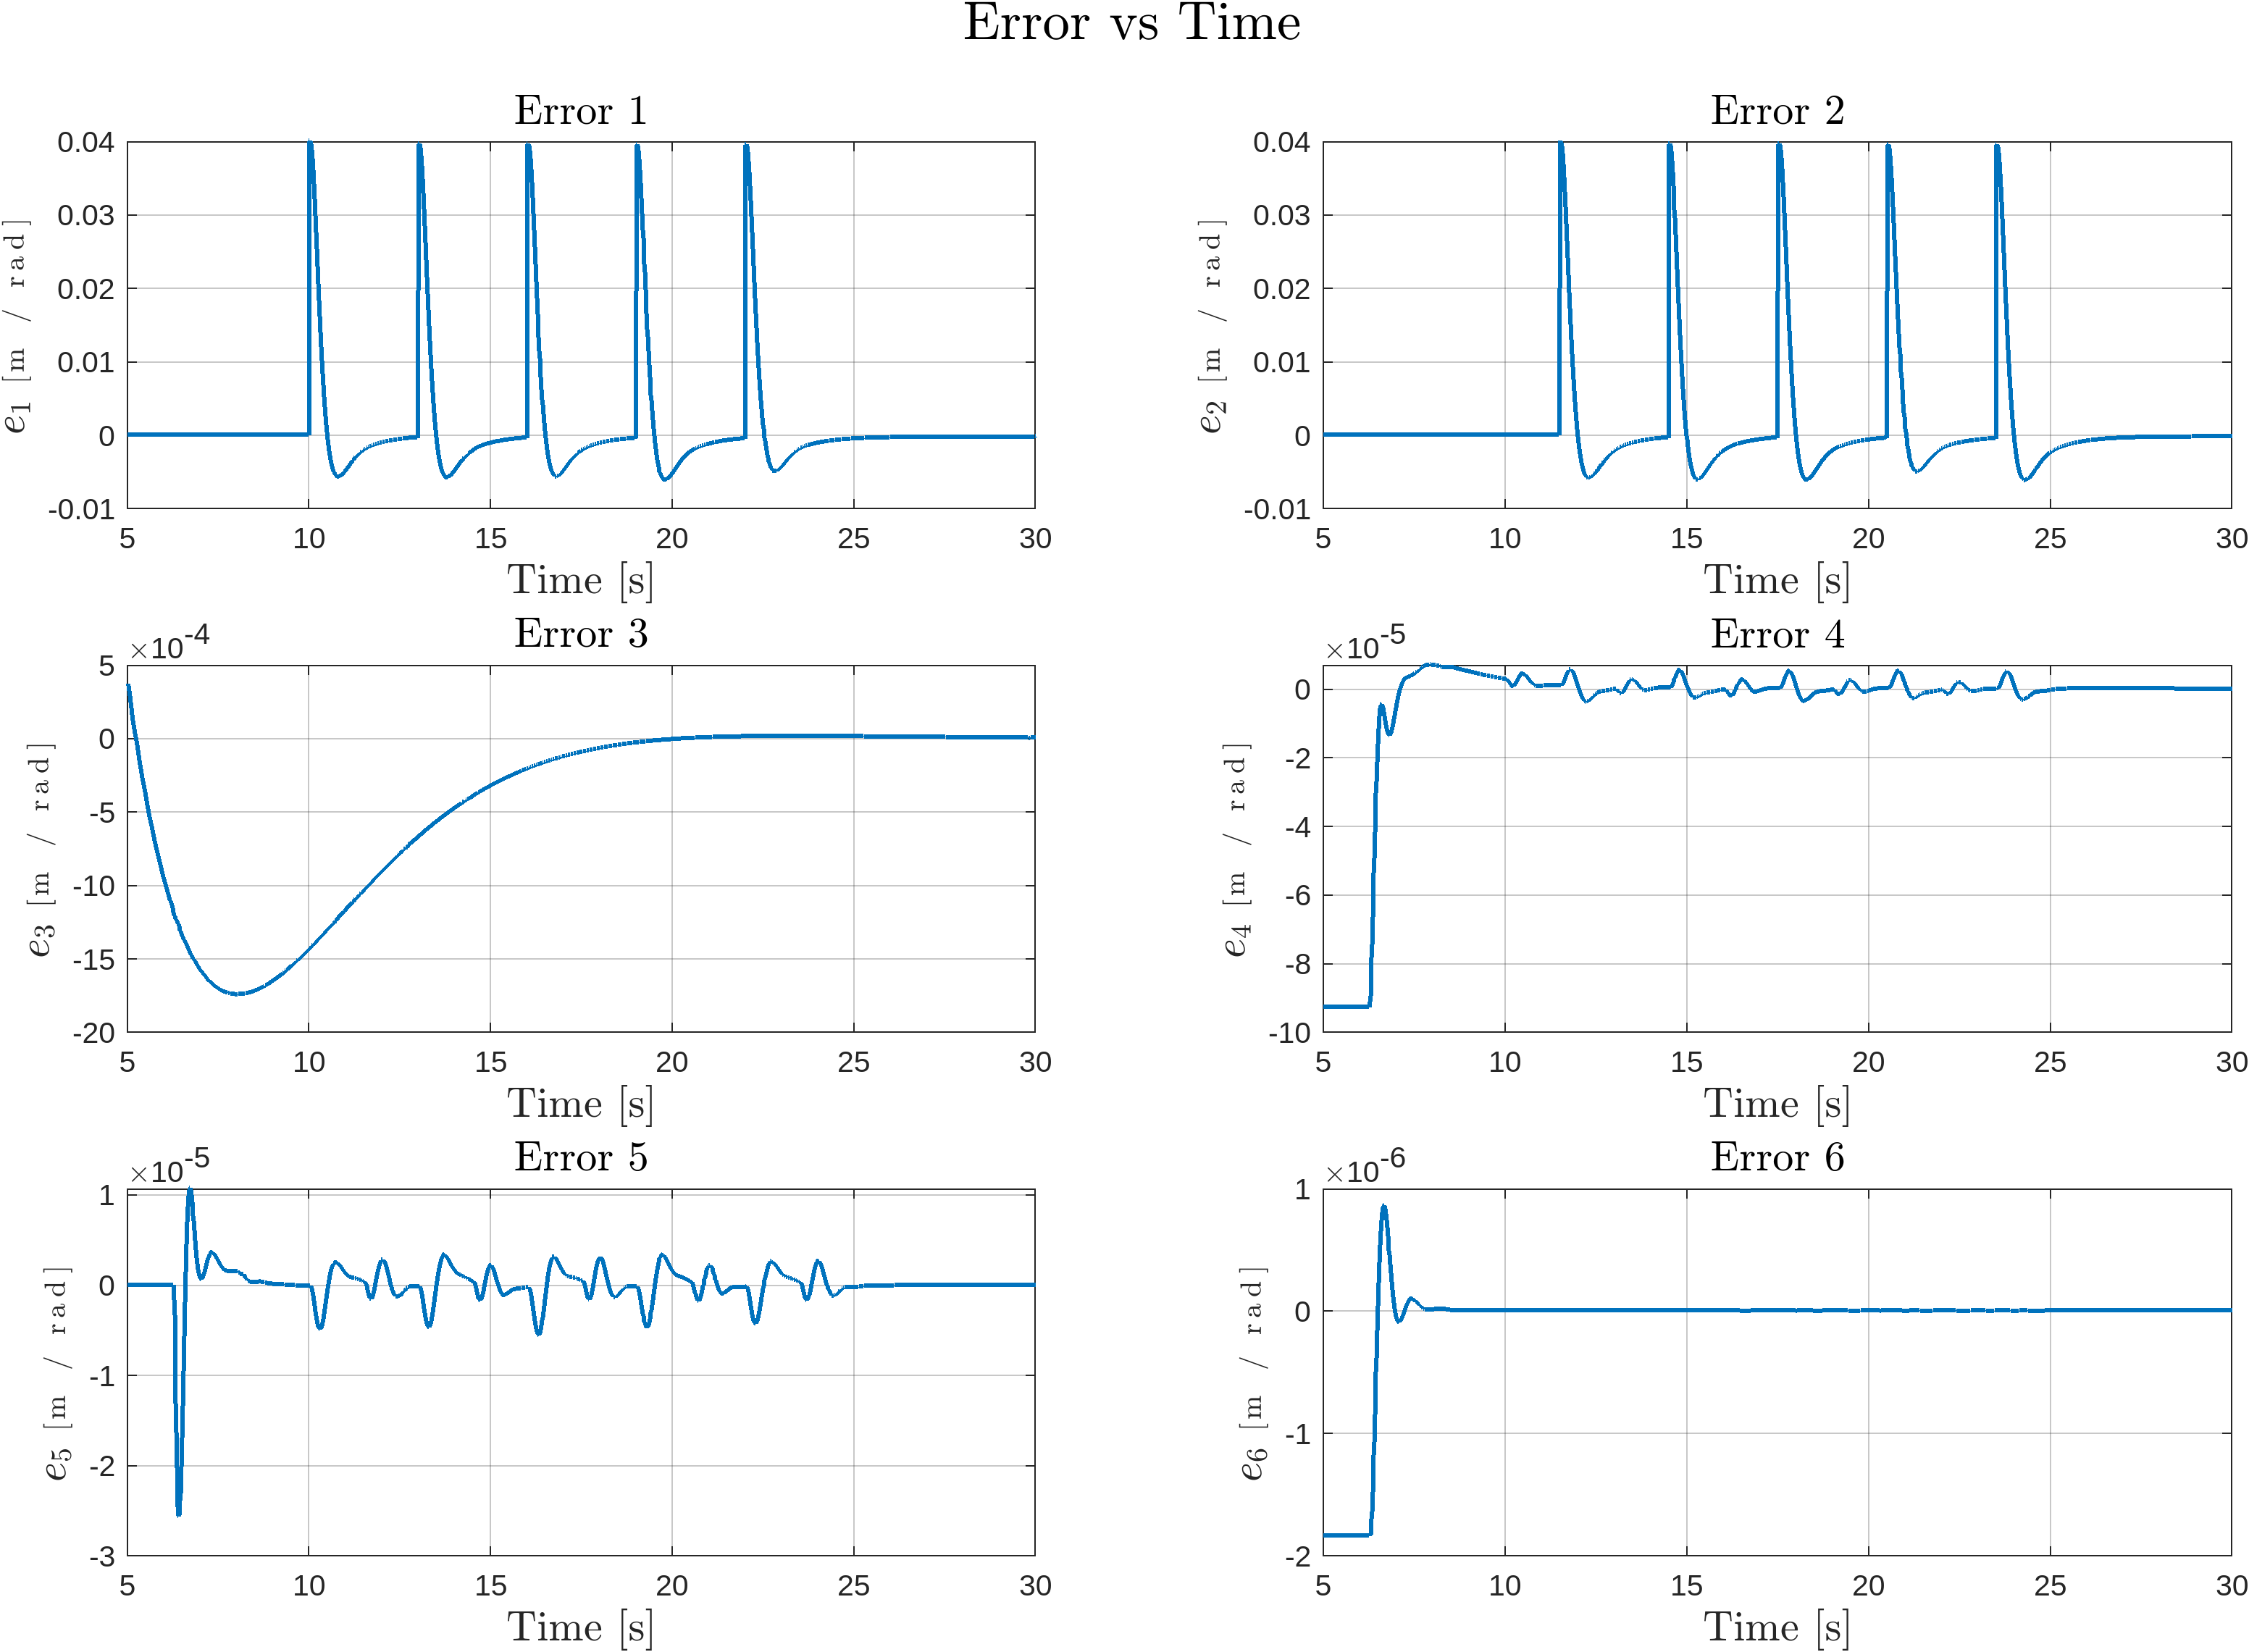
\includegraphics[width=0.7\textwidth]{img/manhattan/15/error}
	\caption{سیگنال خطا در آزمون $15$ ثانیه‌ای (محورهای $X$ و $Y$)}
	\label{fig:results-manhattan-15-error}
\end{figure}

\subsubsection{رفتار تطبیقی بهره‌های فازی}
\label{subsubsec:results-manhattan-fuzzy}
در تمامی سرعت‌ها، الگوی کیفی تغییرات بهره‌های $K_p$، $K_i$ و $K_d$ از منطق توصیف‌شده در بخش \ref{sec:method-control-design} پیروی می‌کند: با شروع هر پله، $K_p$ و $K_d$ افزایش و $K_i$ کاهش می‌یابد و سپس با نزدیک شدن به مقصد، روند معکوس طی می‌شود. آنچه در آزمون منهتن به‌طور ویژه نمایان شد، تغییرات تند و با دامنه‌ی درصدی بزرگ در بهره‌ی انتگرال‌گیر در لحظات تغییر جهت است. این جهش‌های انتگرالی بازتابی از تلاش سیستم برای انطباق سریع با انباشتگی یا تخلیه‌ی ناگهانی خطا در این لحظات بحرانی است. با این حال، دقیقاً به دلیل حضور مکانیزم فازی، این افزایش‌ها موقتی بوده و $K_i$ به سرعت پس از استقرار به مقادیر میانی بازمی‌گردد. در حالی که بهره‌های تناسبی و مشتق کماکان پیرو قوانین تعریف‌شده عمل می‌کنند، رفتار انتگرال‌گیر نشان می‌دهد که سیستم فازی قادر است میان تهاجمی بودن در ردیابی و پایداری بلندمدت مصالحه‌ای پویا برقرار سازد.

\subsubsection{پاسخ سایر درجات آزادی و تلاش کنترلی}
\label{subsubsec:results-manhattan-other-dof}
در حین حرکت صفحه‌ای، محور $Z$ با وجود نوسانات کوچک ناشی از کوپلینگ عرضی، ارتفاع خود را با دقت در محدوده‌ی مجاز حفظ کرد که مرهون پیش‌خور گرانش $68$ نیوتنی و بهره‌های نسبتاً بالای کنترل‌کننده‌ی ارتفاع است. زوایای $\alpha$ و $\beta$ نیز تحت اغتشاشات لحظه‌ای قرار گرفتند، اما کنترل‌کننده‌های وضعیت آنها را در محدوده‌ی کمتر از $0.5$ درجه نگاه داشتند. در تمامی آزمون‌ها، تلاش کنترلی (نیروها و گشتاورها) و جریان‌های سیم‌پیچ‌ها در محدوده‌ی مجاز ($\pm 9$ A و نرخ $80$ A/s) باقی ماندند و هیچ‌گاه به کران‌های اشباع نرسیدند، که تأیید می‌کند معماری تخصیص حتی در مانورهای پیچیده‌ی چندمحوره نیز دستورات عملی و ایمن صادر می‌کند.

\subsection{جمع‌بندی آزمون منهتن}
\label{subsec:results-manhattan-summary}
نتایج مسیر منهتن نشان داد که چارچوب کنترلی پیشنهادی قادر است یک مسیر پلکانی چندبخشی را با دقت و تقارن خوبی در صفحه تعقیب کند. مرز عملکرد سیستم عمدتاً توسط زمان تخصیص‌یافته برای هر قطعه تعیین می‌شود: در $t_{\text{seg}} = 0.5$ ثانیه، انباشتگی خطا قابل ملاحظه و مسیر دچار انحراف فزاینده می‌شود؛ در $t_{\text{seg}} = 1.0$ ثانیه، خطا به شدت کاهش یافته و ردیابی قابل قبول می‌گردد؛ و در $t_{\text{seg}} = 1.5$ ثانیه، خطای ردیابی عملاً صفر شده و سیستم مسیر را بی‌نقص دنبال می‌کند. این یافته‌ها ضمن تأیید عملکرد موفق الگوریتم فازی-PID و قیود تخصیص، محدودیت سرعت ذاتی سیستم را نیز مشخص می‌سازند. با توجه به حفظ پایداری، عدم برخورد با اشباع، و مصرف جریان منطقی در تمامی آزمون‌ها، چارچوب حاضر آمادگی لازم برای انتقال به سخت‌افزار فیزیکی را دارد.



